\PassOptionsToPackage{unicode=true}{hyperref} % options for packages loaded elsewhere
\PassOptionsToPackage{hyphens}{url}
%
\documentclass[]{book}
\usepackage{lmodern}
\usepackage{amssymb,amsmath}
\usepackage{ifxetex,ifluatex}
\usepackage{fixltx2e} % provides \textsubscript
\ifnum 0\ifxetex 1\fi\ifluatex 1\fi=0 % if pdftex
  \usepackage[T1]{fontenc}
  \usepackage[utf8]{inputenc}
  \usepackage{textcomp} % provides euro and other symbols
\else % if luatex or xelatex
  \usepackage{unicode-math}
  \defaultfontfeatures{Ligatures=TeX,Scale=MatchLowercase}
\fi
% use upquote if available, for straight quotes in verbatim environments
\IfFileExists{upquote.sty}{\usepackage{upquote}}{}
% use microtype if available
\IfFileExists{microtype.sty}{%
\usepackage[]{microtype}
\UseMicrotypeSet[protrusion]{basicmath} % disable protrusion for tt fonts
}{}
\IfFileExists{parskip.sty}{%
\usepackage{parskip}
}{% else
\setlength{\parindent}{0pt}
\setlength{\parskip}{6pt plus 2pt minus 1pt}
}
\usepackage{hyperref}
\hypersetup{
            pdftitle={Supplemental info about phylodiversity in evolutionary computation},
            pdfauthor={Jose Guadalupe Hernandez, Alexander Lalejini, Emily Dolson},
            pdfborder={0 0 0},
            breaklinks=true}
\urlstyle{same}  % don't use monospace font for urls
\usepackage{color}
\usepackage{fancyvrb}
\newcommand{\VerbBar}{|}
\newcommand{\VERB}{\Verb[commandchars=\\\{\}]}
\DefineVerbatimEnvironment{Highlighting}{Verbatim}{commandchars=\\\{\}}
% Add ',fontsize=\small' for more characters per line
\usepackage{framed}
\definecolor{shadecolor}{RGB}{248,248,248}
\newenvironment{Shaded}{\begin{snugshade}}{\end{snugshade}}
\newcommand{\AlertTok}[1]{\textcolor[rgb]{0.94,0.16,0.16}{#1}}
\newcommand{\AnnotationTok}[1]{\textcolor[rgb]{0.56,0.35,0.01}{\textbf{\textit{#1}}}}
\newcommand{\AttributeTok}[1]{\textcolor[rgb]{0.77,0.63,0.00}{#1}}
\newcommand{\BaseNTok}[1]{\textcolor[rgb]{0.00,0.00,0.81}{#1}}
\newcommand{\BuiltInTok}[1]{#1}
\newcommand{\CharTok}[1]{\textcolor[rgb]{0.31,0.60,0.02}{#1}}
\newcommand{\CommentTok}[1]{\textcolor[rgb]{0.56,0.35,0.01}{\textit{#1}}}
\newcommand{\CommentVarTok}[1]{\textcolor[rgb]{0.56,0.35,0.01}{\textbf{\textit{#1}}}}
\newcommand{\ConstantTok}[1]{\textcolor[rgb]{0.00,0.00,0.00}{#1}}
\newcommand{\ControlFlowTok}[1]{\textcolor[rgb]{0.13,0.29,0.53}{\textbf{#1}}}
\newcommand{\DataTypeTok}[1]{\textcolor[rgb]{0.13,0.29,0.53}{#1}}
\newcommand{\DecValTok}[1]{\textcolor[rgb]{0.00,0.00,0.81}{#1}}
\newcommand{\DocumentationTok}[1]{\textcolor[rgb]{0.56,0.35,0.01}{\textbf{\textit{#1}}}}
\newcommand{\ErrorTok}[1]{\textcolor[rgb]{0.64,0.00,0.00}{\textbf{#1}}}
\newcommand{\ExtensionTok}[1]{#1}
\newcommand{\FloatTok}[1]{\textcolor[rgb]{0.00,0.00,0.81}{#1}}
\newcommand{\FunctionTok}[1]{\textcolor[rgb]{0.00,0.00,0.00}{#1}}
\newcommand{\ImportTok}[1]{#1}
\newcommand{\InformationTok}[1]{\textcolor[rgb]{0.56,0.35,0.01}{\textbf{\textit{#1}}}}
\newcommand{\KeywordTok}[1]{\textcolor[rgb]{0.13,0.29,0.53}{\textbf{#1}}}
\newcommand{\NormalTok}[1]{#1}
\newcommand{\OperatorTok}[1]{\textcolor[rgb]{0.81,0.36,0.00}{\textbf{#1}}}
\newcommand{\OtherTok}[1]{\textcolor[rgb]{0.56,0.35,0.01}{#1}}
\newcommand{\PreprocessorTok}[1]{\textcolor[rgb]{0.56,0.35,0.01}{\textit{#1}}}
\newcommand{\RegionMarkerTok}[1]{#1}
\newcommand{\SpecialCharTok}[1]{\textcolor[rgb]{0.00,0.00,0.00}{#1}}
\newcommand{\SpecialStringTok}[1]{\textcolor[rgb]{0.31,0.60,0.02}{#1}}
\newcommand{\StringTok}[1]{\textcolor[rgb]{0.31,0.60,0.02}{#1}}
\newcommand{\VariableTok}[1]{\textcolor[rgb]{0.00,0.00,0.00}{#1}}
\newcommand{\VerbatimStringTok}[1]{\textcolor[rgb]{0.31,0.60,0.02}{#1}}
\newcommand{\WarningTok}[1]{\textcolor[rgb]{0.56,0.35,0.01}{\textbf{\textit{#1}}}}
\usepackage{longtable,booktabs}
% Fix footnotes in tables (requires footnote package)
\IfFileExists{footnote.sty}{\usepackage{footnote}\makesavenoteenv{longtable}}{}
\usepackage{graphicx,grffile}
\makeatletter
\def\maxwidth{\ifdim\Gin@nat@width>\linewidth\linewidth\else\Gin@nat@width\fi}
\def\maxheight{\ifdim\Gin@nat@height>\textheight\textheight\else\Gin@nat@height\fi}
\makeatother
% Scale images if necessary, so that they will not overflow the page
% margins by default, and it is still possible to overwrite the defaults
% using explicit options in \includegraphics[width, height, ...]{}
\setkeys{Gin}{width=\maxwidth,height=\maxheight,keepaspectratio}
\setlength{\emergencystretch}{3em}  % prevent overfull lines
\providecommand{\tightlist}{%
  \setlength{\itemsep}{0pt}\setlength{\parskip}{0pt}}
\setcounter{secnumdepth}{5}
% Redefines (sub)paragraphs to behave more like sections
\ifx\paragraph\undefined\else
\let\oldparagraph\paragraph
\renewcommand{\paragraph}[1]{\oldparagraph{#1}\mbox{}}
\fi
\ifx\subparagraph\undefined\else
\let\oldsubparagraph\subparagraph
\renewcommand{\subparagraph}[1]{\oldsubparagraph{#1}\mbox{}}
\fi

% set default figure placement to htbp
\makeatletter
\def\fps@figure{htbp}
\makeatother

\usepackage{booktabs}
\usepackage{longtable}
\usepackage{array}
\usepackage{multirow}
\usepackage{wrapfig}
\usepackage{float}
\usepackage{colortbl}
\usepackage{pdflscape}
\usepackage{tabu}
\usepackage{threeparttable}
\usepackage{threeparttablex}
\usepackage[normalem]{ulem}
\usepackage{makecell}
\usepackage{xcolor}
\usepackage[]{natbib}
\bibliographystyle{apalike}

\title{Supplemental info about phylodiversity in evolutionary computation}
\author{Jose Guadalupe Hernandez, Alexander Lalejini, Emily Dolson}
\date{2021-09-05}

\begin{document}
\maketitle

{
\setcounter{tocdepth}{1}
\tableofcontents
}
\hypertarget{introduction}{%
\chapter{Introduction}\label{introduction}}

This is the supplemental material for our work, \href{https://arxiv.org/abs/2108.12586}{`What can phylogenetic metrics tell us about useful diversity in evolutionary algorithms?'}.
This is not intended as a stand-alone document, but as a companion to our paper.

\hypertarget{about-our-supplemental-material}{%
\section{About our supplemental material}\label{about-our-supplemental-material}}

As you may have noticed (unless you're reading a pdf version of this), our supplemental material is hosted using \href{https://pages.github.com/}{GitHub pages}.
We compiled our data analyses and supplemental documentation into this nifty web-accessible book using \href{https://bookdown.org}{bookdown}.

The source code/configuration files for this supplemental material and all experiments in the paper can be found in \href{https://github.com/emilydolson/phylodiversity-metrics-in-EC-GPTP-2021}{this GitHub repository}.

Our supplemental material includes the following:

TODO

\hypertarget{contributing-authors}{%
\section{Contributing authors}\label{contributing-authors}}

\begin{itemize}
\tightlist
\item
  \href{https://jgh9094.github.io/}{Jose Guadalupe Hernandez}
\item
  \href{https://lalejini.com/}{Alexander Lalejini}
\item
  \href{http://emilyldolson.com/}{Emily Dolson}
\end{itemize}

\hypertarget{research-overview}{%
\section{Research overview}\label{research-overview}}

\hypertarget{abstract}{%
\subsection{Abstract}\label{abstract}}

\begin{quote}
**It is generally accepted that ``diversity'' is associated with success in evolutionary algorithms. However, diversity is a broad concept that can be measured and defined in a multitude of ways. To date, most evolutionary computation research has measured diversity using the richness and/or evenness of a particular genotypic or phenotypic property. While these metrics are informative, we hypothesize that other diversity metrics are more strongly predictive of success. Phylogenetic diversity metrics are a class of metrics popularly used in biology, which take into account the evolutionary history of a population. Here, we investigate the extent to which 1) these metrics provide different information than those traditionally used in evolutionary computation, and 2) these metrics better predict the long-term success of a run of evolutionary computation. We find that, in most cases, phylogenetic metrics behave meaningfully differently from other diversity metrics. Moreover, our results suggest that phylogenetic diversity is indeed a better predictor of success.
\end{quote}

\hypertarget{exploration-diagnostic}{%
\chapter{Exploration Diagnostic}\label{exploration-diagnostic}}

\hypertarget{setup}{%
\section{Setup}\label{setup}}

Include dependencies

\begin{Shaded}
\begin{Highlighting}[]
\KeywordTok{library}\NormalTok{(ggplot2)       }\CommentTok{# For plotting}
\KeywordTok{library}\NormalTok{(tidyverse)     }\CommentTok{# For data wrangling}
\KeywordTok{library}\NormalTok{(knitr)         }\CommentTok{# For making nice rmarkdown documents}
\KeywordTok{library}\NormalTok{(cowplot)       }\CommentTok{# For theme}
\KeywordTok{library}\NormalTok{(viridis)       }\CommentTok{# For color scale}
\KeywordTok{library}\NormalTok{(RColorBrewer)  }\CommentTok{# For more color scales}
\KeywordTok{library}\NormalTok{(rstatix)}
\KeywordTok{library}\NormalTok{(ggsignif)      }\CommentTok{# For adding pairwise significance to plots}
\KeywordTok{library}\NormalTok{(Hmisc)         }\CommentTok{# For bootstrapping condifence internvals}
\KeywordTok{library}\NormalTok{(kableExtra)    }\CommentTok{# For displaying nice tables}
\KeywordTok{source}\NormalTok{(}\StringTok{"https://gist.githubusercontent.com/benmarwick/2a1bb0133ff568cbe28d/raw/fb53bd97121f7f9ce947837ef1a4c65a73bffb3f/geom_flat_violin.R"}\NormalTok{) }\CommentTok{# For raincloud plots}
\KeywordTok{library}\NormalTok{(readr)        }\CommentTok{# For reading in data}
\KeywordTok{library}\NormalTok{(stringr)      }\CommentTok{# For manipulating string data}
\KeywordTok{library}\NormalTok{(ggpubr)       }\CommentTok{# For displaying correlation statistics on plots}
\KeywordTok{library}\NormalTok{(infotheo)     }\CommentTok{# For causality analysis}
\KeywordTok{library}\NormalTok{(scales)       }\CommentTok{# For displaying scales nicely in facetted plots}
\KeywordTok{library}\NormalTok{(osfr)         }\CommentTok{# For downloading the data for this project}
\end{Highlighting}
\end{Shaded}

These analyses were conducted in the following computing environment:

\begin{Shaded}
\begin{Highlighting}[]
\KeywordTok{print}\NormalTok{(version)}
\end{Highlighting}
\end{Shaded}

\begin{verbatim}
##                _                           
## platform       x86_64-pc-linux-gnu         
## arch           x86_64                      
## os             linux-gnu                   
## system         x86_64, linux-gnu           
## status                                     
## major          4                           
## minor          0.4                         
## year           2021                        
## month          02                          
## day            15                          
## svn rev        80002                       
## language       R                           
## version.string R version 4.0.4 (2021-02-15)
## nickname       Lost Library Book
\end{verbatim}

Setup constants to be used across plots

\begin{Shaded}
\begin{Highlighting}[]
\CommentTok{# Labeler for stats annotations}
\NormalTok{p_label <-}\StringTok{ }\ControlFlowTok{function}\NormalTok{(p_value) \{}
\NormalTok{  threshold =}\StringTok{ }\FloatTok{0.0001}
  \ControlFlowTok{if}\NormalTok{ (p_value }\OperatorTok{<}\StringTok{ }\NormalTok{threshold) \{}
    \KeywordTok{return}\NormalTok{(}\KeywordTok{paste0}\NormalTok{(}\StringTok{"p < "}\NormalTok{, threshold))}
\NormalTok{  \} }\ControlFlowTok{else}\NormalTok{ \{}
    \KeywordTok{return}\NormalTok{(}\KeywordTok{paste0}\NormalTok{(}\StringTok{"p = "}\NormalTok{, p_value))}
\NormalTok{  \}}
\NormalTok{\}}

\CommentTok{# Significance threshold}
\NormalTok{alpha <-}\StringTok{ }\FloatTok{0.05}

\CommentTok{# Common graph variables}
\NormalTok{performance_ylim <-}\StringTok{ }\DecValTok{1}
\NormalTok{coverage_ylim <-}\StringTok{ }\FloatTok{1.0}

\CommentTok{####### misc #######}
\CommentTok{# Configure our default graphing theme}
\KeywordTok{theme_set}\NormalTok{(}\KeywordTok{theme_cowplot}\NormalTok{())}
\end{Highlighting}
\end{Shaded}

\begin{Shaded}
\begin{Highlighting}[]
\CommentTok{# Read in data}
\KeywordTok{osf_retrieve_file}\NormalTok{(}\StringTok{"esm4r"}\NormalTok{) }\OperatorTok\StringTok{ }\KeywordTok{osf_download}\NormalTok{(}\DataTypeTok{conflicts =} \StringTok{"skip"}\NormalTok{)  }\CommentTok{# Download data from osf}
\end{Highlighting}
\end{Shaded}

\begin{verbatim}
## # A tibble: 1 x 4
##   name                    id               local_path                meta       
##   <chr>                   <chr>            <chr>                     <list>     
## 1 final_exploration_diag~ 612fe97aab8bca0~ ./final_exploration_diag~ <named lis~
\end{verbatim}

\begin{Shaded}
\begin{Highlighting}[]
\NormalTok{data_loc <-}\StringTok{ "final_exploration_diagnostic_data.csv"}

\NormalTok{data <-}\StringTok{ }\KeywordTok{read_csv}\NormalTok{(data_loc, }\DataTypeTok{na=}\KeywordTok{c}\NormalTok{(}\StringTok{"NONE"}\NormalTok{, }\StringTok{"NA"}\NormalTok{, }\StringTok{""}\NormalTok{))}

\CommentTok{## Clean up data columns}

\CommentTok{# Make selection name column human readable}
\NormalTok{data <-}\StringTok{ }\NormalTok{data }\OperatorTok\StringTok{ }\KeywordTok{mutate}\NormalTok{(}\DataTypeTok{selection_name =} \KeywordTok{as.factor}\NormalTok{(}\KeywordTok{case_when}\NormalTok{(}
\NormalTok{  selection_name }\OperatorTok{==}\StringTok{ "EpsilonLexicase"} \OperatorTok{~}\StringTok{ "Lexicase"}\NormalTok{,}
\NormalTok{  TOUR_SIZE }\OperatorTok{==}\StringTok{ }\DecValTok{1} \OperatorTok{~}\StringTok{ "Random"}\NormalTok{,}
\NormalTok{  selection_name }\OperatorTok{==}\StringTok{ "Tournament"} \OperatorTok{~}\StringTok{ "Tournament"}\NormalTok{,}
\NormalTok{  selection_name }\OperatorTok{==}\StringTok{ "FitnessSharing"} \OperatorTok{~}\StringTok{ "Fitness Sharing"}\NormalTok{,}
\NormalTok{  selection_name }\OperatorTok{==}\StringTok{ "EcoEa"} \OperatorTok{~}\StringTok{ "EcoEA"}
\NormalTok{)))}

\CommentTok{# Calculate performance statistics.}
\CommentTok{# Elite trait avg is the avg per-site performance of the best individual}
\NormalTok{data}\OperatorTok{$}\NormalTok{elite_trait_avg <-}
\StringTok{  }\NormalTok{data}\OperatorTok{$}\NormalTok{ele_agg_per }\OperatorTok{/}\StringTok{ }\NormalTok{data}\OperatorTok{$}\NormalTok{OBJECTIVE_CNT}
\NormalTok{data}\OperatorTok{$}\NormalTok{unique_start_positions_coverage <-}
\StringTok{  }\NormalTok{data}\OperatorTok{$}\NormalTok{uni_str_pos }\OperatorTok{/}\StringTok{ }\NormalTok{data}\OperatorTok{$}\NormalTok{OBJECTIVE_CNT}

\CommentTok{# Convert elite_trait_avg to percent of maximum possible}
\NormalTok{data}\OperatorTok{$}\NormalTok{elite_trait_avg <-}\StringTok{ }\NormalTok{data}\OperatorTok{$}\NormalTok{elite_trait_avg}\OperatorTok{/}\NormalTok{data}\OperatorTok{$}\NormalTok{TARGET}

\CommentTok{# Grab data from just the final time point}
\NormalTok{final_data <-}\StringTok{ }\KeywordTok{filter}\NormalTok{(data, evaluations}\OperatorTok{==}\KeywordTok{max}\NormalTok{(data}\OperatorTok{$}\NormalTok{evaluations))}
\end{Highlighting}
\end{Shaded}

\hypertarget{performance}{%
\section{Performance}\label{performance}}

For context, it's important to know how each selection scheme performed on the exploration diagnostic.

\hypertarget{over-time}{%
\subsection{Over time}\label{over-time}}

First we look at the dynamics of performance over time.

\hypertarget{trait-performance}{%
\subsubsection{Trait performance}\label{trait-performance}}

Plot average trait performance (i.e.~fitness) over time for each selection scheme. We log the x-axis because Eco-EA gains fitness over a very long time scale, whereas the interesting dynamics for the other selection schemes occur relatively quickly.

\begin{Shaded}
\begin{Highlighting}[]
\KeywordTok{ggplot}\NormalTok{(}
\NormalTok{    data,}
    \KeywordTok{aes}\NormalTok{(}
      \DataTypeTok{x=}\NormalTok{gen,                 }\CommentTok{# Generations}
      \DataTypeTok{y=}\NormalTok{elite_trait_avg,     }\CommentTok{# Performance}
      \DataTypeTok{color=}\NormalTok{selection_name,  }\CommentTok{# Selection scheme}
      \DataTypeTok{fill=}\NormalTok{selection_name}
\NormalTok{    )}
\NormalTok{  ) }\OperatorTok{+}
\StringTok{  }\KeywordTok{stat_summary}\NormalTok{(}\DataTypeTok{geom=}\StringTok{"line"}\NormalTok{, }\DataTypeTok{fun=}\NormalTok{mean) }\OperatorTok{+}\StringTok{ }\CommentTok{# Plot line showing mean for each selection scheme}
\StringTok{  }\KeywordTok{stat_summary}\NormalTok{(  }\CommentTok{# Add shading around each line indicating 95% confiedence interval}
    \DataTypeTok{geom=}\StringTok{"ribbon"}\NormalTok{,}
    \DataTypeTok{fun.data=}\StringTok{"mean_cl_boot"}\NormalTok{,}
    \DataTypeTok{fun.args=}\KeywordTok{list}\NormalTok{(}\DataTypeTok{conf.int=}\FloatTok{0.95}\NormalTok{),}
    \DataTypeTok{alpha=}\FloatTok{0.2}\NormalTok{,}
    \DataTypeTok{linetype=}\DecValTok{0}
\NormalTok{  ) }\OperatorTok{+}
\StringTok{  }\KeywordTok{scale_y_continuous}\NormalTok{(}
    \DataTypeTok{name=}\StringTok{"Average trait performance"}\NormalTok{, }\CommentTok{# Set y axis title}
    \DataTypeTok{limits=}\KeywordTok{c}\NormalTok{(}\DecValTok{0}\NormalTok{, performance_ylim)  }\CommentTok{# Set y axis range to include all possible performance values}
\NormalTok{  ) }\OperatorTok{+}
\StringTok{  }\KeywordTok{scale_x_log10}\NormalTok{(  }\CommentTok{# Log x axis}
    \DataTypeTok{name=}\StringTok{"Generation"} \CommentTok{# Set x axis title}
\NormalTok{  ) }\OperatorTok{+}
\StringTok{  }\KeywordTok{scale_color_discrete}\NormalTok{(}\StringTok{"Selection"}\NormalTok{) }\OperatorTok{+}\StringTok{ }\CommentTok{# Set legend title}
\StringTok{  }\KeywordTok{scale_fill_discrete}\NormalTok{(}\StringTok{"Selection"}\NormalTok{)    }\CommentTok{# Set legend title}
\end{Highlighting}
\end{Shaded}

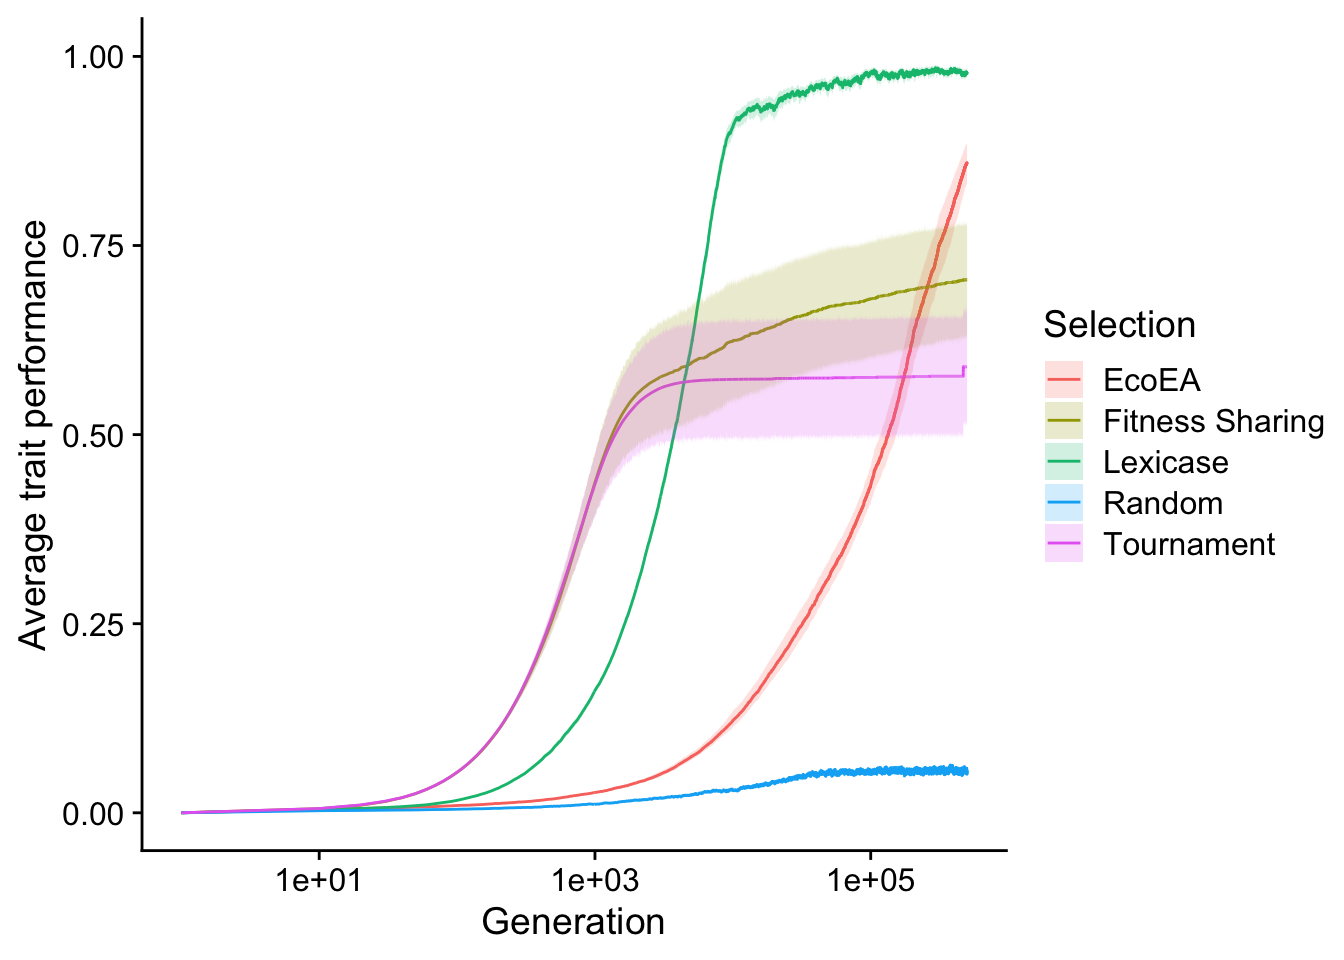
\includegraphics{phylodiversity-in-EC-supplement_files/figure-latex/performance_over_time-1.pdf}

As observed by Hernandez et al.~in their original paper on the exploration diagnostic, fitness in tournament selection initially increases quickly and then plateaus. Fitness in lexicase selection increases slightly slower but plateaus at a much higher value (nearly 100\%). Fitness sharing behaves similarly to tournament selection, but maintains a slight upward trajectory (note that, because the x axis is on a log scale, this trajectory is very gradual). Eco-EA takes substantially longer to increase in fitness but ultimately surpasses fitness sharing and tournament selection. It is unclear whether it would pass lexicase selection if these runs were allowed to continue for slightly longer; they do not appear to have plateaued yet. We chose to cut them off at 500,000 generations due to resource constraints and the fact that the questions we're asking here are not really about final fitness.

\hypertarget{activation-position-coverage}{%
\subsubsection{Activation position coverage}\label{activation-position-coverage}}

Out of curiosity, we also ran the analysis of unique activation positions present in the population, used by Hernandez et. al.~This analysis tells us about the diversity of start positions for the coding region represented in the population. As the set of start positions in the population tends to represent a meaningful constraint on the number of paths through the fitness landscape that are currently accessible, this is in some sense a metric of useful diversity in the population

\begin{Shaded}
\begin{Highlighting}[]
\KeywordTok{ggplot}\NormalTok{(data, }\KeywordTok{aes}\NormalTok{(}\DataTypeTok{x=}\NormalTok{gen, }\DataTypeTok{y=}\NormalTok{unique_start_positions_coverage, }\DataTypeTok{color=}\NormalTok{selection_name, }\DataTypeTok{fill=}\NormalTok{selection_name)) }\OperatorTok{+}
\StringTok{  }\KeywordTok{stat_summary}\NormalTok{(}\DataTypeTok{geom=}\StringTok{"line"}\NormalTok{, }\DataTypeTok{fun=}\NormalTok{mean) }\OperatorTok{+}
\StringTok{  }\KeywordTok{stat_summary}\NormalTok{(}
    \DataTypeTok{geom=}\StringTok{"ribbon"}\NormalTok{,}
    \DataTypeTok{fun.data=}\StringTok{"mean_cl_boot"}\NormalTok{,}
    \DataTypeTok{fun.args=}\KeywordTok{list}\NormalTok{(}\DataTypeTok{conf.int=}\FloatTok{0.95}\NormalTok{),}
    \DataTypeTok{alpha=}\FloatTok{0.2}\NormalTok{,}
    \DataTypeTok{linetype=}\DecValTok{0}
\NormalTok{  ) }\OperatorTok{+}
\StringTok{  }\KeywordTok{scale_y_continuous}\NormalTok{(}
    \DataTypeTok{name=}\StringTok{"Activation position coverage"}\NormalTok{,}
    \DataTypeTok{limits=}\KeywordTok{c}\NormalTok{(}\DecValTok{0}\NormalTok{, }\DecValTok{100}\NormalTok{)}
\NormalTok{  ) }\OperatorTok{+}
\StringTok{  }\KeywordTok{scale_x_log10}\NormalTok{(}
    \DataTypeTok{name=}\StringTok{"Generation"}
\NormalTok{  ) }\OperatorTok{+}
\StringTok{  }\KeywordTok{scale_color_discrete}\NormalTok{(}\StringTok{"Selection"}\NormalTok{)}\OperatorTok{+}
\StringTok{  }\KeywordTok{scale_fill_discrete}\NormalTok{(}\StringTok{"Selection"}\NormalTok{)}
\end{Highlighting}
\end{Shaded}

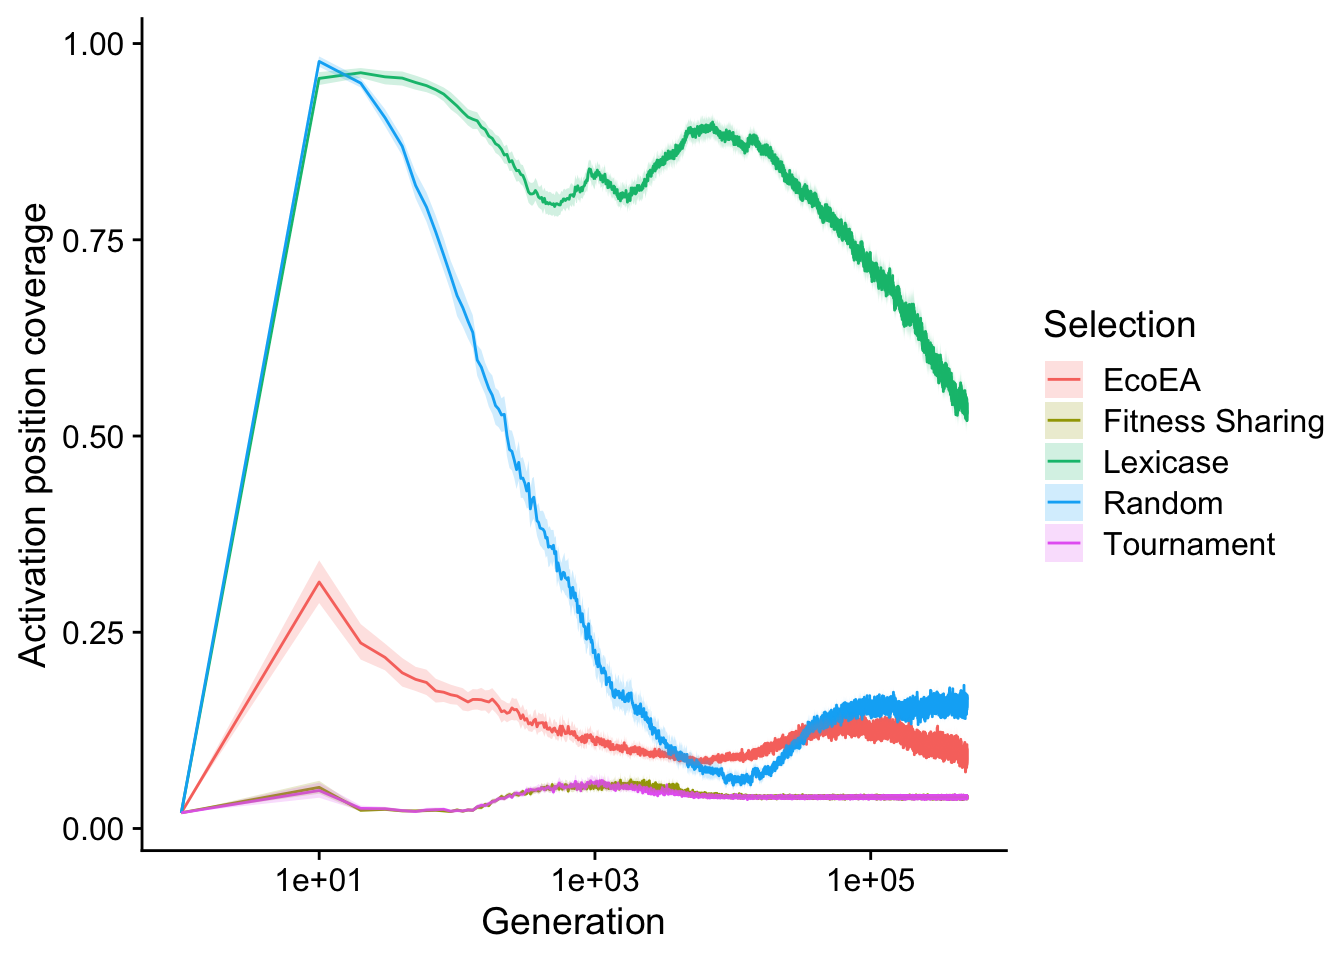
\includegraphics{phylodiversity-in-EC-supplement_files/figure-latex/unique_start_positions-1.pdf}

We see that lexicase selection maintains by far that largest number of unique start positions, even surpassing the number maintained by random drift. This suggests that lexicase selection is actively selecting for maintaining a diversity of start positions. Tournament selection and fitness sharing perform virtually identically, with Eco-EA falling in between.

\hypertarget{final}{%
\subsection{Final}\label{final}}

While trends over time are more informative, it can be hard to visualize the full distribution (particularly the extent of variation). Thus, we also conduct a more detailed analysis of performance at the final time point.

\hypertarget{trait-performance-1}{%
\subsubsection{Trait performance}\label{trait-performance-1}}

First we conduct statistics to identify which selection schemes are significantly different from each other.

\begin{Shaded}
\begin{Highlighting}[]
\CommentTok{# Compute manual labels for geom_signif}
\NormalTok{stat.test <-}\StringTok{ }\NormalTok{final_data }\OperatorTok
\StringTok{  }\KeywordTok{wilcox_test}\NormalTok{(elite_trait_avg }\OperatorTok{~}\StringTok{ }\NormalTok{selection_name) }\OperatorTok
\StringTok{  }\KeywordTok{adjust_pvalue}\NormalTok{(}\DataTypeTok{method =} \StringTok{"bonferroni"}\NormalTok{) }\OperatorTok\StringTok{  }\CommentTok{# Apply Bonferroni correction for multiple comparisons}
\StringTok{  }\KeywordTok{add_significance}\NormalTok{() }\OperatorTok
\StringTok{  }\KeywordTok{add_xy_position}\NormalTok{(}\DataTypeTok{x=}\StringTok{"selection_name"}\NormalTok{,}\DataTypeTok{step.increase=}\DecValTok{1}\NormalTok{)}
\NormalTok{stat.test}\OperatorTok{$}\NormalTok{label <-}\StringTok{ }\KeywordTok{mapply}\NormalTok{(p_label,stat.test}\OperatorTok{$}\NormalTok{p.adj)}
\end{Highlighting}
\end{Shaded}

Then we make raincloud plots of each selection scheme.

\begin{Shaded}
\begin{Highlighting}[]
\NormalTok{elite_final_performance_fig <-}\StringTok{ }\KeywordTok{ggplot}\NormalTok{(}
\NormalTok{    final_data,}
    \KeywordTok{aes}\NormalTok{(}
      \DataTypeTok{x=}\NormalTok{selection_name,}
      \DataTypeTok{y=}\NormalTok{elite_trait_avg,}
      \DataTypeTok{fill=}\NormalTok{selection_name}
\NormalTok{    )}
\NormalTok{  ) }\OperatorTok{+}
\StringTok{  }\KeywordTok{geom_flat_violin}\NormalTok{(}
    \DataTypeTok{position =} \KeywordTok{position_nudge}\NormalTok{(}\DataTypeTok{x =} \FloatTok{.2}\NormalTok{, }\DataTypeTok{y =} \DecValTok{0}\NormalTok{),}
    \DataTypeTok{alpha =} \FloatTok{.8}\NormalTok{,}
    \DataTypeTok{scale=}\StringTok{"width"}
\NormalTok{  ) }\OperatorTok{+}
\StringTok{  }\KeywordTok{geom_point}\NormalTok{(}
    \DataTypeTok{mapping=}\KeywordTok{aes}\NormalTok{(}\DataTypeTok{color=}\NormalTok{selection_name),}
    \DataTypeTok{position =} \KeywordTok{position_jitter}\NormalTok{(}\DataTypeTok{width =} \FloatTok{.15}\NormalTok{),}
    \DataTypeTok{size =} \FloatTok{.5}\NormalTok{,}
    \DataTypeTok{alpha =} \FloatTok{0.8}
\NormalTok{  ) }\OperatorTok{+}
\StringTok{  }\KeywordTok{geom_boxplot}\NormalTok{(}
    \DataTypeTok{width =} \FloatTok{.1}\NormalTok{,}
    \DataTypeTok{outlier.shape =} \OtherTok{NA}\NormalTok{,}
    \DataTypeTok{alpha =} \FloatTok{0.5}
\NormalTok{  ) }\OperatorTok{+}
\StringTok{  }\KeywordTok{scale_y_continuous}\NormalTok{(}
    \DataTypeTok{name=}\StringTok{"Average trait performance"}\NormalTok{,}
    \DataTypeTok{limits=}\KeywordTok{c}\NormalTok{(}\DecValTok{0}\NormalTok{, performance_ylim)}
\NormalTok{  ) }\OperatorTok{+}
\StringTok{  }\KeywordTok{scale_x_discrete}\NormalTok{(}
    \DataTypeTok{name=}\StringTok{"Selection"}
\NormalTok{  ) }\OperatorTok{+}
\StringTok{  }\KeywordTok{scale_fill_discrete}\NormalTok{(}
    \DataTypeTok{name=}\StringTok{"Selection"}
\NormalTok{  ) }\OperatorTok{+}
\StringTok{  }\KeywordTok{scale_color_discrete}\NormalTok{(}
    \DataTypeTok{name=}\StringTok{"Selection"}
\NormalTok{  ) }\OperatorTok{+}\StringTok{ }
\StringTok{  }\KeywordTok{theme}\NormalTok{(}\DataTypeTok{legend.position=}\StringTok{"none"}\NormalTok{)}
\NormalTok{elite_final_performance_fig}
\end{Highlighting}
\end{Shaded}

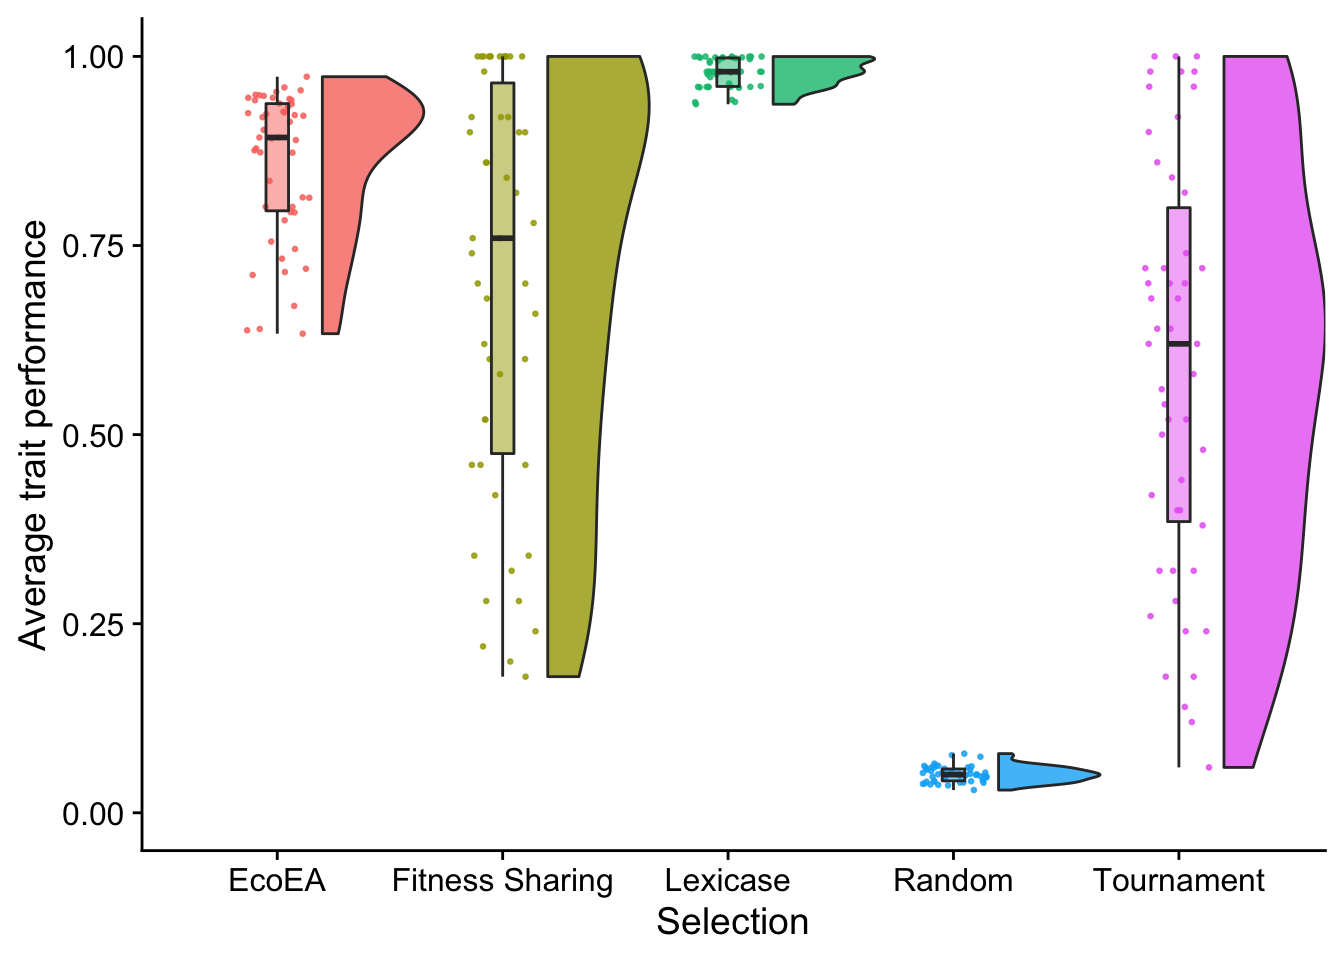
\includegraphics{phylodiversity-in-EC-supplement_files/figure-latex/final_performance_plot-1.pdf}

These observations look fairly consistent with the timeseries plots.

Next, we output the results of our significance testing.

\begin{Shaded}
\begin{Highlighting}[]
\NormalTok{stat.test }\OperatorTok
\StringTok{  }\KeywordTok{kbl}\NormalTok{() }\OperatorTok
\StringTok{  }\KeywordTok{kable_styling}\NormalTok{(}
    \DataTypeTok{bootstrap_options =} \KeywordTok{c}\NormalTok{(}
      \StringTok{"striped"}\NormalTok{,}
      \StringTok{"hover"}\NormalTok{,}
      \StringTok{"condensed"}\NormalTok{,}
      \StringTok{"responsive"}
\NormalTok{    )}
\NormalTok{  ) }\OperatorTok
\StringTok{  }\KeywordTok{scroll_box}\NormalTok{(}\DataTypeTok{width=}\StringTok{"600px"}\NormalTok{)}
\end{Highlighting}
\end{Shaded}

\begin{table}
\centering
\begin{tabular}[t]{l|l|l|r|r|r|r|r|l|r|l|r|r|l}
\hline
.y. & group1 & group2 & n1 & n2 & statistic & p & p.adj & p.adj.signif & y.position & groups & xmin & xmax & label\\
\hline
elite\_trait\_avg & EcoEA & Fitness Sharing & 50 & 50 & 1561 & 3.20e-02 & 3.20e-01 & ns & 1.922000 & EcoEA          , Fitness Sharing & 1 & 2 & p = 0.32\\
\hline
elite\_trait\_avg & EcoEA & Lexicase & 50 & 47 & 60 & 0.00e+00 & 0.00e+00 & **** & 2.946444 & EcoEA   , Lexicase & 1 & 3 & p < 1e-04\\
\hline
elite\_trait\_avg & EcoEA & Random & 50 & 50 & 2500 & 0.00e+00 & 0.00e+00 & **** & 3.970889 & EcoEA , Random & 1 & 4 & p < 1e-04\\
\hline
elite\_trait\_avg & EcoEA & Tournament & 50 & 50 & 1939 & 2.10e-06 & 2.07e-05 & **** & 4.995333 & EcoEA     , Tournament & 1 & 5 & p < 1e-04\\
\hline
elite\_trait\_avg & Fitness Sharing & Lexicase & 50 & 47 & 593 & 2.69e-05 & 2.69e-04 & *** & 6.019778 & Fitness Sharing, Lexicase & 2 & 3 & p = 0.000269\\
\hline
elite\_trait\_avg & Fitness Sharing & Random & 50 & 50 & 2500 & 0.00e+00 & 0.00e+00 & **** & 7.044222 & Fitness Sharing, Random & 2 & 4 & p < 1e-04\\
\hline
elite\_trait\_avg & Fitness Sharing & Tournament & 50 & 50 & 1549 & 4.00e-02 & 4.00e-01 & ns & 8.068667 & Fitness Sharing, Tournament & 2 & 5 & p = 0.4\\
\hline
elite\_trait\_avg & Lexicase & Random & 47 & 50 & 2350 & 0.00e+00 & 0.00e+00 & **** & 9.093111 & Lexicase, Random & 3 & 4 & p < 1e-04\\
\hline
elite\_trait\_avg & Lexicase & Tournament & 47 & 50 & 2098 & 0.00e+00 & 0.00e+00 & **** & 10.117556 & Lexicase  , Tournament & 3 & 5 & p < 1e-04\\
\hline
elite\_trait\_avg & Random & Tournament & 50 & 50 & 10 & 0.00e+00 & 0.00e+00 & **** & 11.142000 & Random    , Tournament & 4 & 5 & p < 1e-04\\
\hline
\end{tabular}
\end{table}

\hypertarget{final-activation-position-coverage}{%
\subsubsection{Final activation position Coverage}\label{final-activation-position-coverage}}

Now we do the same analysis for final activation position coverage.

First we calculate the statistics

\begin{Shaded}
\begin{Highlighting}[]
\CommentTok{# Compute manual labels for geom_signif}
\NormalTok{stat.test <-}\StringTok{ }\NormalTok{final_data }\OperatorTok
\StringTok{  }\KeywordTok{wilcox_test}\NormalTok{(unique_start_positions_coverage }\OperatorTok{~}\StringTok{ }\NormalTok{selection_name) }\OperatorTok
\StringTok{  }\KeywordTok{adjust_pvalue}\NormalTok{(}\DataTypeTok{method =} \StringTok{"bonferroni"}\NormalTok{) }\OperatorTok
\StringTok{  }\KeywordTok{add_significance}\NormalTok{() }\OperatorTok
\StringTok{  }\KeywordTok{add_xy_position}\NormalTok{(}\DataTypeTok{x=}\StringTok{"selection_name"}\NormalTok{,}\DataTypeTok{step.increase=}\DecValTok{1}\NormalTok{)}
\NormalTok{stat.test}\OperatorTok{$}\NormalTok{manual_position <-}\StringTok{ }\NormalTok{stat.test}\OperatorTok{$}\NormalTok{y.position }\OperatorTok{*}\StringTok{ }\FloatTok{1.05}
\NormalTok{stat.test}\OperatorTok{$}\NormalTok{label <-}\StringTok{ }\KeywordTok{mapply}\NormalTok{(p_label,stat.test}\OperatorTok{$}\NormalTok{p.adj)}
\end{Highlighting}
\end{Shaded}

Then we make raincloud plots

\begin{Shaded}
\begin{Highlighting}[]
\NormalTok{unique_start_positions_coverage_final_fig <-}\StringTok{ }\KeywordTok{ggplot}\NormalTok{(}
\NormalTok{    final_data,}
    \KeywordTok{aes}\NormalTok{(}
      \DataTypeTok{x=}\NormalTok{selection_name,}
      \DataTypeTok{y=}\NormalTok{unique_start_positions_coverage,}
      \DataTypeTok{fill=}\NormalTok{selection_name}
\NormalTok{    )}
\NormalTok{  ) }\OperatorTok{+}
\StringTok{  }\KeywordTok{geom_flat_violin}\NormalTok{(}
    \DataTypeTok{position =} \KeywordTok{position_nudge}\NormalTok{(}\DataTypeTok{x =} \FloatTok{.2}\NormalTok{, }\DataTypeTok{y =} \DecValTok{0}\NormalTok{),}
    \DataTypeTok{alpha =} \FloatTok{.8}\NormalTok{,}
    \DataTypeTok{scale=}\StringTok{"width"}
\NormalTok{  ) }\OperatorTok{+}
\StringTok{  }\KeywordTok{geom_point}\NormalTok{(}
    \DataTypeTok{mapping=}\KeywordTok{aes}\NormalTok{(}\DataTypeTok{color=}\NormalTok{selection_name),}
    \DataTypeTok{position =} \KeywordTok{position_jitter}\NormalTok{(}\DataTypeTok{width =} \FloatTok{.15}\NormalTok{),}
    \DataTypeTok{size =} \FloatTok{.5}\NormalTok{,}
    \DataTypeTok{alpha =} \FloatTok{0.8}
\NormalTok{  ) }\OperatorTok{+}
\StringTok{  }\KeywordTok{geom_boxplot}\NormalTok{(}
    \DataTypeTok{width =} \FloatTok{.1}\NormalTok{,}
    \DataTypeTok{outlier.shape =} \OtherTok{NA}\NormalTok{,}
    \DataTypeTok{alpha =} \FloatTok{0.5}
\NormalTok{  ) }\OperatorTok{+}
\StringTok{  }\KeywordTok{scale_y_continuous}\NormalTok{(}
    \DataTypeTok{name=}\StringTok{"Activation position coverage"}\NormalTok{,}
    \DataTypeTok{limits=}\KeywordTok{c}\NormalTok{(}\DecValTok{0}\NormalTok{, coverage_ylim)}
\NormalTok{  ) }\OperatorTok{+}
\StringTok{  }\KeywordTok{scale_x_discrete}\NormalTok{(}
    \DataTypeTok{name=}\StringTok{"Selection"}
\NormalTok{  ) }\OperatorTok{+}
\StringTok{  }\KeywordTok{scale_fill_discrete}\NormalTok{(}
    \DataTypeTok{name=}\StringTok{"Selection"}
\NormalTok{  ) }\OperatorTok{+}
\StringTok{  }\KeywordTok{scale_color_discrete}\NormalTok{(}
    \DataTypeTok{name=}\StringTok{"Selection"}
\NormalTok{  ) }\OperatorTok{+}
\StringTok{  }\KeywordTok{theme}\NormalTok{(}
    \DataTypeTok{legend.position=}\StringTok{"none"}
\NormalTok{  )}
\NormalTok{unique_start_positions_coverage_final_fig}
\end{Highlighting}
\end{Shaded}

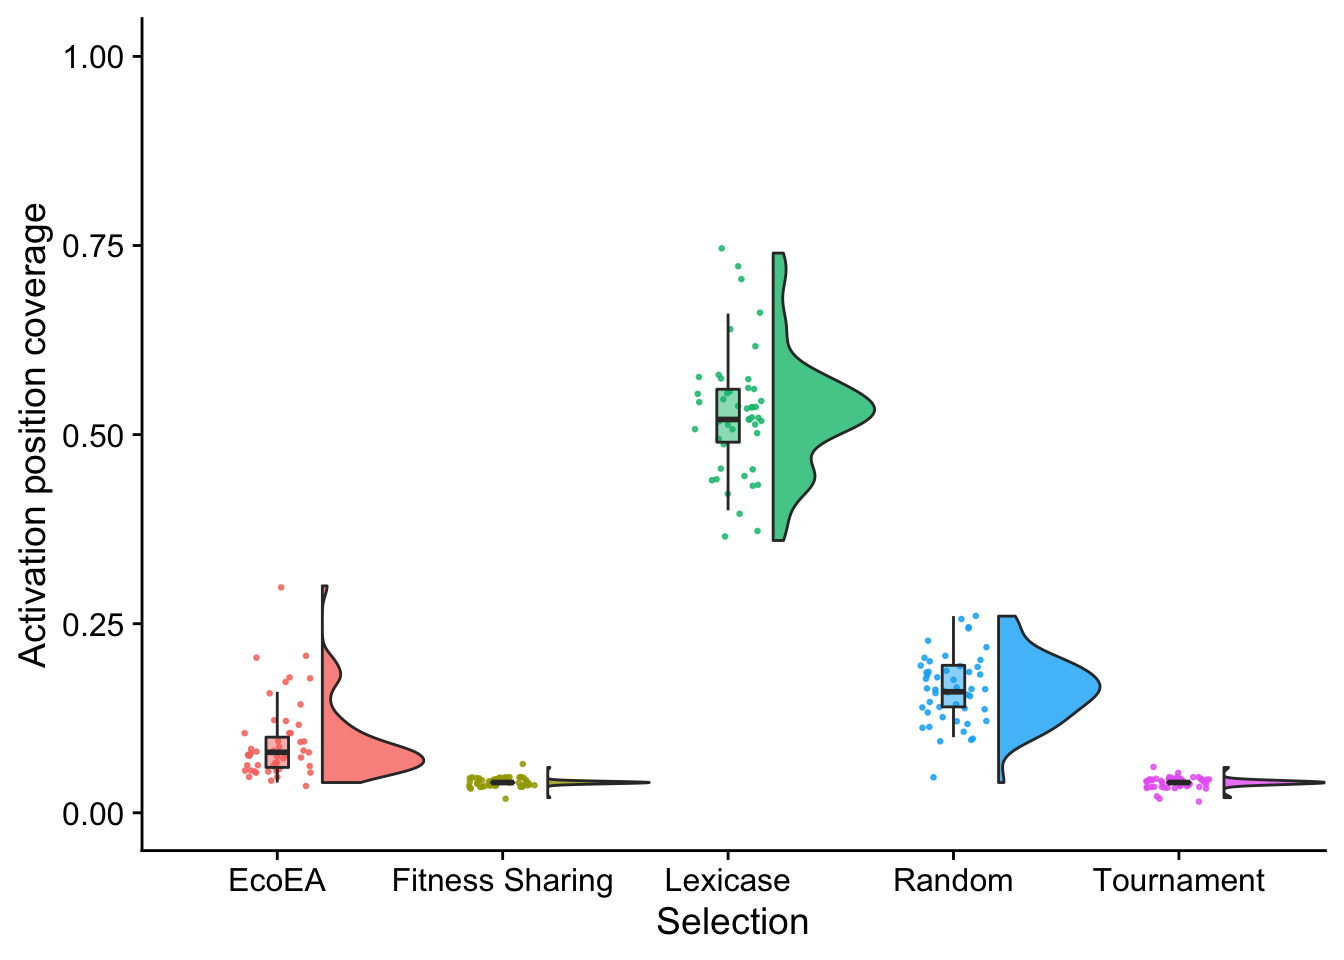
\includegraphics{phylodiversity-in-EC-supplement_files/figure-latex/unique_start_positions_final-1.pdf}

These also look unsurprising.

Lastly, we output the results of significance testing.

\begin{Shaded}
\begin{Highlighting}[]
\NormalTok{stat.test }\OperatorTok
\StringTok{  }\KeywordTok{kbl}\NormalTok{() }\OperatorTok
\StringTok{  }\KeywordTok{kable_styling}\NormalTok{(}
    \DataTypeTok{bootstrap_options =} \KeywordTok{c}\NormalTok{(}
      \StringTok{"striped"}\NormalTok{,}
      \StringTok{"hover"}\NormalTok{,}
      \StringTok{"condensed"}\NormalTok{,}
      \StringTok{"responsive"}
\NormalTok{    )}
\NormalTok{  ) }\OperatorTok
\StringTok{  }\KeywordTok{scroll_box}\NormalTok{(}\DataTypeTok{width=}\StringTok{"600px"}\NormalTok{)}
\end{Highlighting}
\end{Shaded}

\begin{table}
\centering
\begin{tabular}[t]{l|l|l|r|r|r|r|r|l|r|l|r|r|r|l}
\hline
.y. & group1 & group2 & n1 & n2 & statistic & p & p.adj & p.adj.signif & y.position & groups & xmin & xmax & manual\_position & label\\
\hline
unique\_start\_positions\_coverage & EcoEA & Fitness Sharing & 50 & 50 & 2392.5 & 0.000 & 0 & **** & 1.420000 & EcoEA          , Fitness Sharing & 1 & 2 & 1.491000 & p < 1e-04\\
\hline
unique\_start\_positions\_coverage & EcoEA & Lexicase & 50 & 47 & 0.0 & 0.000 & 0 & **** & 2.175556 & EcoEA   , Lexicase & 1 & 3 & 2.284333 & p < 1e-04\\
\hline
unique\_start\_positions\_coverage & EcoEA & Random & 50 & 50 & 339.0 & 0.000 & 0 & **** & 2.931111 & EcoEA , Random & 1 & 4 & 3.077667 & p < 1e-04\\
\hline
unique\_start\_positions\_coverage & EcoEA & Tournament & 50 & 50 & 2387.0 & 0.000 & 0 & **** & 3.686667 & EcoEA     , Tournament & 1 & 5 & 3.871000 & p < 1e-04\\
\hline
unique\_start\_positions\_coverage & Fitness Sharing & Lexicase & 50 & 47 & 0.0 & 0.000 & 0 & **** & 4.442222 & Fitness Sharing, Lexicase & 2 & 3 & 4.664333 & p < 1e-04\\
\hline
unique\_start\_positions\_coverage & Fitness Sharing & Random & 50 & 50 & 25.0 & 0.000 & 0 & **** & 5.197778 & Fitness Sharing, Random & 2 & 4 & 5.457667 & p < 1e-04\\
\hline
unique\_start\_positions\_coverage & Fitness Sharing & Tournament & 50 & 50 & 1274.5 & 0.708 & 1 & ns & 5.953333 & Fitness Sharing, Tournament & 2 & 5 & 6.251000 & p = 1\\
\hline
unique\_start\_positions\_coverage & Lexicase & Random & 47 & 50 & 2350.0 & 0.000 & 0 & **** & 6.708889 & Lexicase, Random & 3 & 4 & 7.044333 & p < 1e-04\\
\hline
unique\_start\_positions\_coverage & Lexicase & Tournament & 47 & 50 & 2350.0 & 0.000 & 0 & **** & 7.464444 & Lexicase  , Tournament & 3 & 5 & 7.837667 & p < 1e-04\\
\hline
unique\_start\_positions\_coverage & Random & Tournament & 50 & 50 & 2475.5 & 0.000 & 0 & **** & 8.220000 & Random    , Tournament & 4 & 5 & 8.631000 & p < 1e-04\\
\hline
\end{tabular}
\end{table}

\hypertarget{phylogenetic-diversity}{%
\section{Phylogenetic diversity}\label{phylogenetic-diversity}}

Next, we analyze the behavior of phylogenetic diversity on the exploration diagnostic.

\hypertarget{over-time-1}{%
\subsection{Over time}\label{over-time-1}}

First we plot mean pairwise distance over time. We log the y axis because there is such variation in mean pairwise distance across selection schemes.

\begin{Shaded}
\begin{Highlighting}[]
\KeywordTok{ggplot}\NormalTok{(}
\NormalTok{    data,}
    \KeywordTok{aes}\NormalTok{(}
      \DataTypeTok{x=}\NormalTok{gen,}
      \DataTypeTok{y=}\NormalTok{mean_phenotype_pairwise_distance,}
      \DataTypeTok{color=}\NormalTok{selection_name,}
      \DataTypeTok{fill=}\NormalTok{selection_name}
\NormalTok{    )}
\NormalTok{  ) }\OperatorTok{+}
\StringTok{  }\KeywordTok{stat_summary}\NormalTok{(}\DataTypeTok{geom=}\StringTok{"line"}\NormalTok{, }\DataTypeTok{fun=}\NormalTok{mean) }\OperatorTok{+}
\StringTok{  }\KeywordTok{stat_summary}\NormalTok{(}
    \DataTypeTok{geom=}\StringTok{"ribbon"}\NormalTok{,}
    \DataTypeTok{fun.data=}\StringTok{"mean_cl_boot"}\NormalTok{,}
    \DataTypeTok{fun.args=}\KeywordTok{list}\NormalTok{(}\DataTypeTok{conf.int=}\FloatTok{0.95}\NormalTok{),}
    \DataTypeTok{alpha=}\FloatTok{0.2}\NormalTok{,}
    \DataTypeTok{linetype=}\DecValTok{0}
\NormalTok{  ) }\OperatorTok{+}
\StringTok{  }\KeywordTok{scale_y_log10}\NormalTok{(}
    \DataTypeTok{name=}\StringTok{"Mean pairwise distance"}
\NormalTok{  ) }\OperatorTok{+}
\StringTok{  }\KeywordTok{scale_x_log10}\NormalTok{(}
    \DataTypeTok{name=}\StringTok{"Generation"}
\NormalTok{  ) }\OperatorTok{+}
\StringTok{  }\KeywordTok{scale_color_discrete}\NormalTok{(}\StringTok{"Selection"}\NormalTok{) }\OperatorTok{+}
\StringTok{  }\KeywordTok{scale_fill_discrete}\NormalTok{(}\StringTok{"Selection"}\NormalTok{)}
\end{Highlighting}
\end{Shaded}

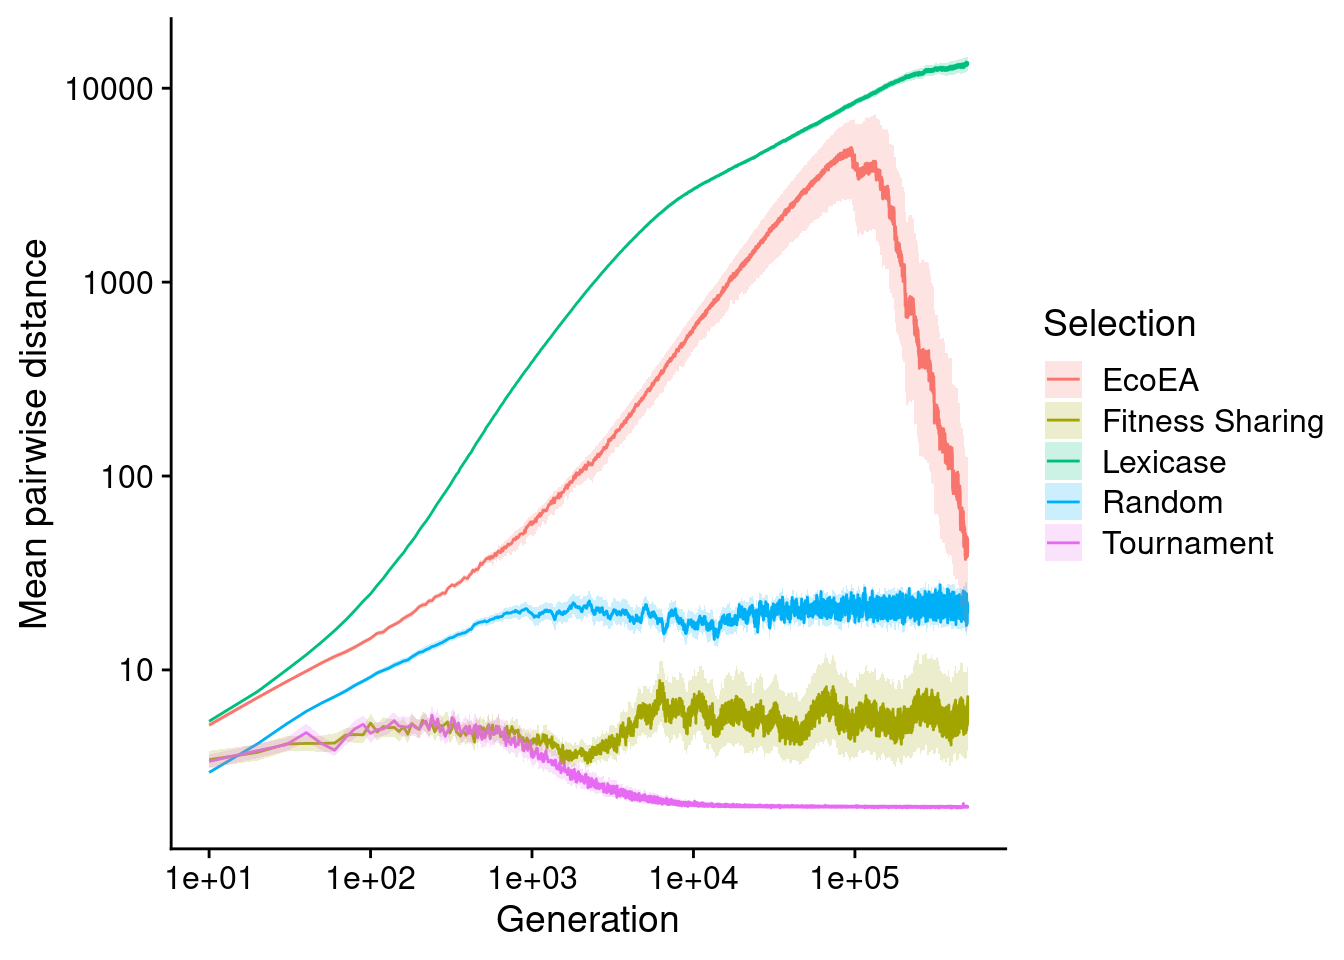
\includegraphics{phylodiversity-in-EC-supplement_files/figure-latex/phylogeny_over_time_plot_mpd-1.pdf}

Lexicase selection maintains a monotonic increase in phylogenetic diversity over the course of the entire experiment. It likely never experiences a full coalesence event (where the most-recent common ancestor changes). Eco-EA nearly keeps pace with lexicase selection until towards the end, when its phylogenetic diversity crashes. This is likely the result of selective sweeps that begin to occur as the population discovers high fitness solutions. Fitness sharing shows a slight dip at the same time that its fitness plateaus (likely also the result of a selective sweep), but phylogenetic diversity recovers afterwards, making for a relatively constant level. over time. Tournament selection, on the other hand, maintains the same (low) level of phylogenetic diversity as fitness sharing, up until the point that fitness plateaus, at which point tournament selection's phylodiversity drops to nearly 0. Interestingly, lexicase selection and Eco-EA both maintain more phylodiversity than random selection, whereas fitness sharing and tournament selection maintain less.

For comparison, we make the same plot with mean evolutionary distinctiveness.

\begin{Shaded}
\begin{Highlighting}[]
\KeywordTok{ggplot}\NormalTok{(}
\NormalTok{    data,}
    \KeywordTok{aes}\NormalTok{(}
      \DataTypeTok{x=}\NormalTok{gen,}
      \DataTypeTok{y=}\NormalTok{mean_phenotype_evolutionary_distinctiveness,}
      \DataTypeTok{color=}\NormalTok{selection_name,}
      \DataTypeTok{fill=}\NormalTok{selection_name}
\NormalTok{    )}
\NormalTok{  ) }\OperatorTok{+}
\StringTok{  }\KeywordTok{stat_summary}\NormalTok{(}\DataTypeTok{geom=}\StringTok{"line"}\NormalTok{, }\DataTypeTok{fun=}\NormalTok{mean) }\OperatorTok{+}
\StringTok{  }\KeywordTok{stat_summary}\NormalTok{(}
    \DataTypeTok{geom=}\StringTok{"ribbon"}\NormalTok{,}
    \DataTypeTok{fun.data=}\StringTok{"mean_cl_boot"}\NormalTok{,}
    \DataTypeTok{fun.args=}\KeywordTok{list}\NormalTok{(}\DataTypeTok{conf.int=}\FloatTok{0.95}\NormalTok{),}
    \DataTypeTok{alpha=}\FloatTok{0.2}\NormalTok{,}
    \DataTypeTok{linetype=}\DecValTok{0}
\NormalTok{  ) }\OperatorTok{+}
\StringTok{  }\KeywordTok{scale_y_log10}\NormalTok{(}
    \DataTypeTok{name=}\StringTok{"Mean evolutionary distinctiveness"}
\NormalTok{  ) }\OperatorTok{+}
\StringTok{  }\KeywordTok{scale_x_log10}\NormalTok{(}
    \DataTypeTok{name=}\StringTok{"Generation"}
\NormalTok{  ) }\OperatorTok{+}
\StringTok{  }\KeywordTok{scale_color_discrete}\NormalTok{(}\StringTok{"Selection"}\NormalTok{) }\OperatorTok{+}
\StringTok{  }\KeywordTok{scale_fill_discrete}\NormalTok{(}\StringTok{"Selection"}\NormalTok{)}
\end{Highlighting}
\end{Shaded}

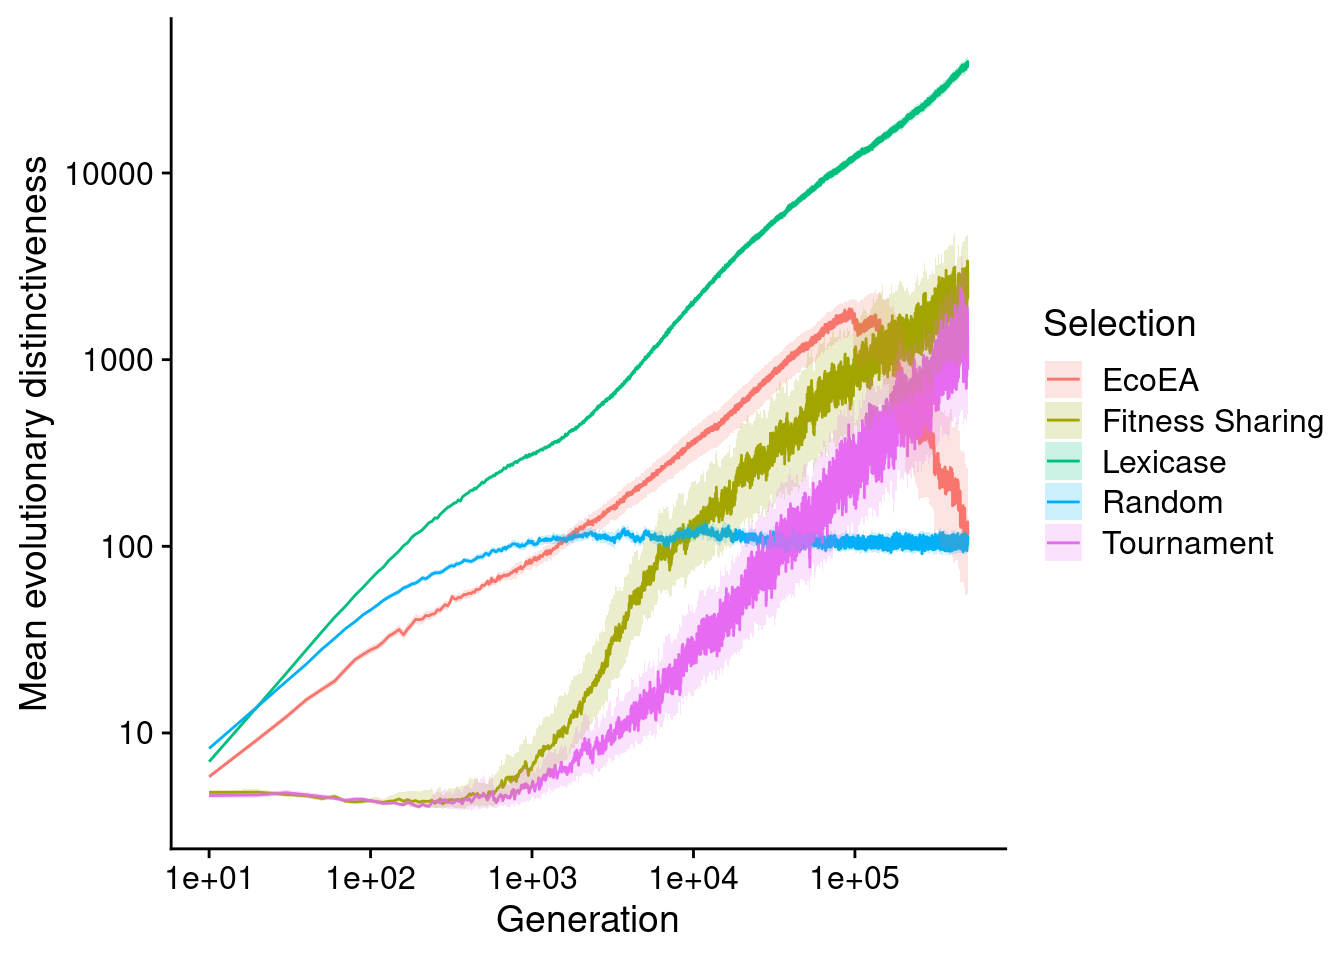
\includegraphics{phylodiversity-in-EC-supplement_files/figure-latex/phylogeny_over_time_plot_med-1.pdf}

\hypertarget{final-1}{%
\subsection{Final}\label{final-1}}

Next, we perform a more in-depth analysis of phylodiversity distributions at the final time point.

\hypertarget{mean-pairwise-distance}{%
\subsubsection{Mean pairwise distance}\label{mean-pairwise-distance}}

\begin{Shaded}
\begin{Highlighting}[]
\CommentTok{# Pairwise wilcoxon teset to determine which conditions are significantly different from each other}
\NormalTok{stat.test <-}\StringTok{ }\NormalTok{final_data }\OperatorTok
\StringTok{  }\KeywordTok{wilcox_test}\NormalTok{(mean_phenotype_pairwise_distance }\OperatorTok{~}\StringTok{ }\NormalTok{selection_name) }\OperatorTok
\StringTok{  }\KeywordTok{adjust_pvalue}\NormalTok{(}\DataTypeTok{method =} \StringTok{"bonferroni"}\NormalTok{) }\OperatorTok
\StringTok{  }\KeywordTok{add_significance}\NormalTok{() }\OperatorTok
\StringTok{  }\KeywordTok{add_xy_position}\NormalTok{(}\DataTypeTok{x=}\StringTok{"selection_name"}\NormalTok{,}\DataTypeTok{step.increase=}\DecValTok{1}\NormalTok{)}
\NormalTok{stat.test}\OperatorTok{$}\NormalTok{label <-}\StringTok{ }\KeywordTok{mapply}\NormalTok{(p_label,stat.test}\OperatorTok{$}\NormalTok{p.adj)}

\CommentTok{# Output stats}
\NormalTok{stat.test }\OperatorTok
\StringTok{  }\KeywordTok{kbl}\NormalTok{() }\OperatorTok
\StringTok{  }\KeywordTok{kable_styling}\NormalTok{(}
    \DataTypeTok{bootstrap_options =} \KeywordTok{c}\NormalTok{(}
      \StringTok{"striped"}\NormalTok{,}
      \StringTok{"hover"}\NormalTok{,}
      \StringTok{"condensed"}\NormalTok{,}
      \StringTok{"responsive"}
\NormalTok{    )}
\NormalTok{  ) }\OperatorTok
\StringTok{  }\KeywordTok{scroll_box}\NormalTok{(}\DataTypeTok{width=}\StringTok{"600px"}\NormalTok{)}
\end{Highlighting}
\end{Shaded}

\begin{table}
\centering
\begin{tabular}[t]{l|l|l|r|r|r|r|r|l|r|l|r|r|l}
\hline
.y. & group1 & group2 & n1 & n2 & statistic & p & p.adj & p.adj.signif & y.position & groups & xmin & xmax & label\\
\hline
mean\_phenotype\_pairwise\_distance & EcoEA & Fitness Sharing & 50 & 50 & 1824.0 & 7.70e-05 & 7.70e-04 & *** & 49488.81 & EcoEA          , Fitness Sharing & 1 & 2 & p = 0.00077\\
\hline
mean\_phenotype\_pairwise\_distance & EcoEA & Lexicase & 50 & 47 & 227.0 & 0.00e+00 & 0.00e+00 & **** & 76981.49 & EcoEA   , Lexicase & 1 & 3 & p < 1e-04\\
\hline
mean\_phenotype\_pairwise\_distance & EcoEA & Random & 50 & 50 & 690.0 & 1.15e-04 & 1.15e-03 & ** & 104474.18 & EcoEA , Random & 1 & 4 & p = 0.00115\\
\hline
mean\_phenotype\_pairwise\_distance & EcoEA & Tournament & 50 & 50 & 2500.0 & 0.00e+00 & 0.00e+00 & **** & 131966.86 & EcoEA     , Tournament & 1 & 5 & p < 1e-04\\
\hline
mean\_phenotype\_pairwise\_distance & Fitness Sharing & Lexicase & 50 & 47 & 0.0 & 0.00e+00 & 0.00e+00 & **** & 159459.54 & Fitness Sharing, Lexicase & 2 & 3 & p < 1e-04\\
\hline
mean\_phenotype\_pairwise\_distance & Fitness Sharing & Random & 50 & 50 & 536.0 & 9.00e-07 & 8.70e-06 & **** & 186952.22 & Fitness Sharing, Random & 2 & 4 & p < 1e-04\\
\hline
mean\_phenotype\_pairwise\_distance & Fitness Sharing & Tournament & 50 & 50 & 2232.5 & 0.00e+00 & 0.00e+00 & **** & 214444.90 & Fitness Sharing, Tournament & 2 & 5 & p < 1e-04\\
\hline
mean\_phenotype\_pairwise\_distance & Lexicase & Random & 47 & 50 & 2350.0 & 0.00e+00 & 0.00e+00 & **** & 241937.58 & Lexicase, Random & 3 & 4 & p < 1e-04\\
\hline
mean\_phenotype\_pairwise\_distance & Lexicase & Tournament & 47 & 50 & 2350.0 & 0.00e+00 & 0.00e+00 & **** & 269430.26 & Lexicase  , Tournament & 3 & 5 & p < 1e-04\\
\hline
mean\_phenotype\_pairwise\_distance & Random & Tournament & 50 & 50 & 2500.0 & 0.00e+00 & 0.00e+00 & **** & 296922.94 & Random    , Tournament & 4 & 5 & p < 1e-04\\
\hline
\end{tabular}
\end{table}

\begin{Shaded}
\begin{Highlighting}[]
\CommentTok{# Raincloud plot of final mean pairwise distance}
\NormalTok{final_phylogeny_fig <-}\StringTok{ }\KeywordTok{ggplot}\NormalTok{(}
\NormalTok{    final_data,}
    \KeywordTok{aes}\NormalTok{(}
      \DataTypeTok{x=}\NormalTok{selection_name,}
      \DataTypeTok{y=}\NormalTok{mean_phenotype_pairwise_distance,}
      \DataTypeTok{fill=}\NormalTok{selection_name}
\NormalTok{    )}
\NormalTok{  ) }\OperatorTok{+}
\StringTok{  }\KeywordTok{geom_flat_violin}\NormalTok{(}
    \DataTypeTok{position =} \KeywordTok{position_nudge}\NormalTok{(}\DataTypeTok{x =} \FloatTok{.2}\NormalTok{, }\DataTypeTok{y =} \DecValTok{0}\NormalTok{),}
    \DataTypeTok{alpha =} \FloatTok{.8}\NormalTok{,}
    \DataTypeTok{scale=}\StringTok{"width"}
\NormalTok{  ) }\OperatorTok{+}
\StringTok{  }\KeywordTok{geom_point}\NormalTok{(}
    \DataTypeTok{mapping=}\KeywordTok{aes}\NormalTok{(}\DataTypeTok{color=}\NormalTok{selection_name),}
    \DataTypeTok{position =} \KeywordTok{position_jitter}\NormalTok{(}\DataTypeTok{width =} \FloatTok{.15}\NormalTok{),}
    \DataTypeTok{size =} \FloatTok{.5}\NormalTok{,}
    \DataTypeTok{alpha =} \FloatTok{0.8}
\NormalTok{  ) }\OperatorTok{+}
\StringTok{  }\KeywordTok{geom_boxplot}\NormalTok{(}
    \DataTypeTok{width =} \FloatTok{.1}\NormalTok{,}
    \DataTypeTok{outlier.shape =} \OtherTok{NA}\NormalTok{,}
    \DataTypeTok{alpha =} \FloatTok{0.5}
\NormalTok{  ) }\OperatorTok{+}
\StringTok{  }\KeywordTok{scale_y_log10}\NormalTok{(}
    \DataTypeTok{name=}\StringTok{"Mean pairwise distance"}
\NormalTok{  ) }\OperatorTok{+}
\StringTok{  }\KeywordTok{scale_x_discrete}\NormalTok{(}
    \DataTypeTok{name=}\StringTok{"Selection"}
\NormalTok{  ) }\OperatorTok{+}
\StringTok{  }\KeywordTok{scale_fill_discrete}\NormalTok{(}
    \DataTypeTok{name=}\StringTok{"Selection"}
\NormalTok{  ) }\OperatorTok{+}
\StringTok{  }\KeywordTok{scale_color_discrete}\NormalTok{(}
    \DataTypeTok{name=}\StringTok{"Selection"}
\NormalTok{  ) }\OperatorTok{+}\StringTok{ }
\StringTok{  }\KeywordTok{theme}\NormalTok{(}\DataTypeTok{legend.position =} \StringTok{"none"}\NormalTok{)}
\NormalTok{final_phylogeny_fig}
\end{Highlighting}
\end{Shaded}

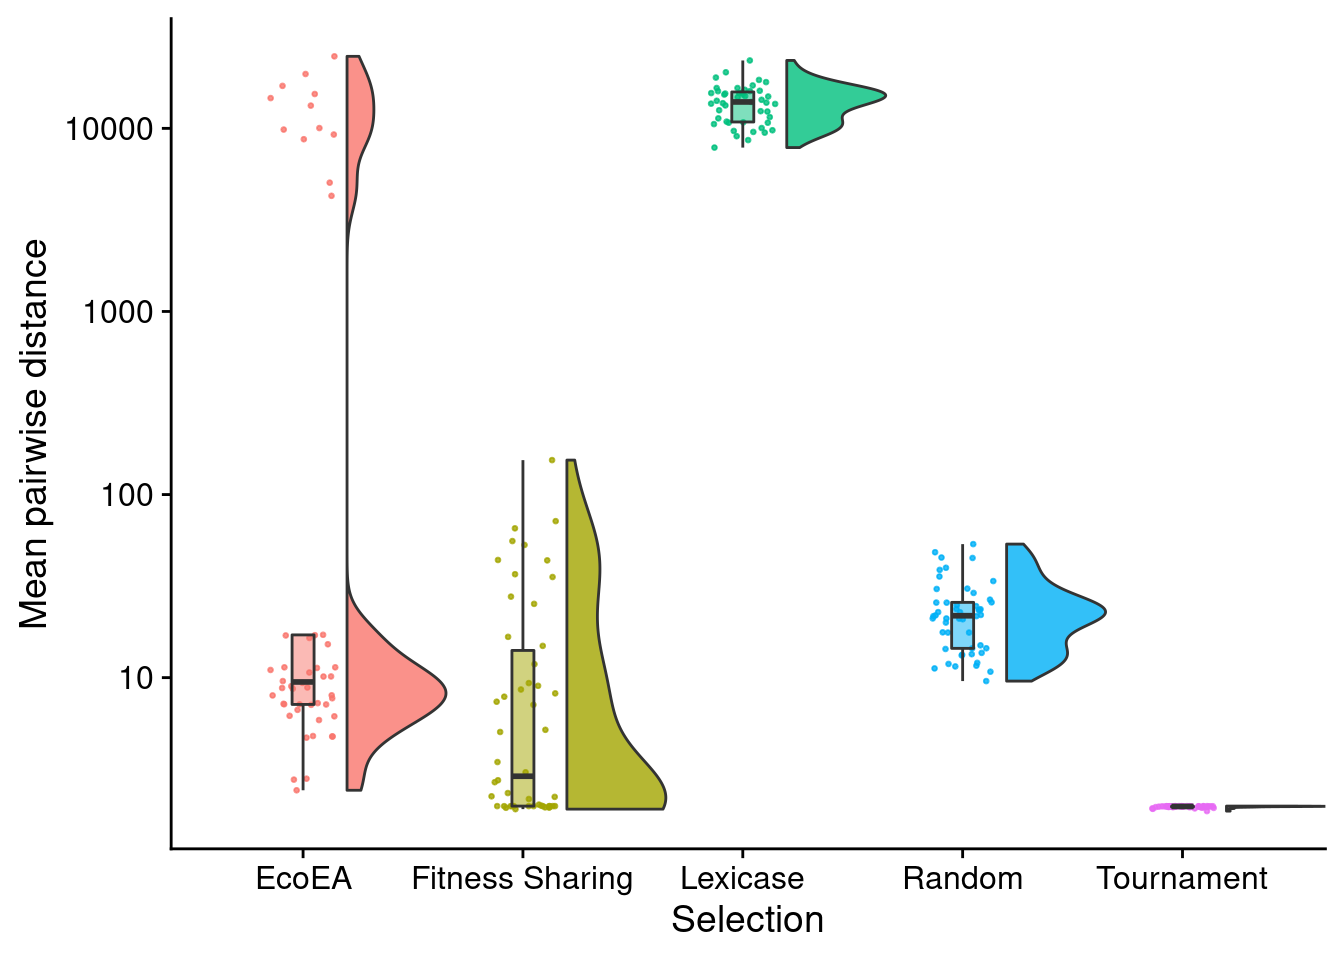
\includegraphics{phylodiversity-in-EC-supplement_files/figure-latex/final_phylogeny_plot_mpd-1.pdf}

This shows something interesting! Final phylogenetic diversity in Eco-EA is heavily bimodal. In later analysis, we will see that the runs with high phylogenetic diversity are the ones with lower fitness, suggesting that they have no yet experienced a selective sweep resulting from the discovery of a high-fitness solution.

\hypertarget{mean-evolutionary-distinctiveness}{%
\subsubsection{Mean evolutionary distinctiveness}\label{mean-evolutionary-distinctiveness}}

\begin{Shaded}
\begin{Highlighting}[]
\CommentTok{# Pairwise wilcoxon teset to determine which conditions are significantly different from each other}
\NormalTok{stat.test <-}\StringTok{ }\NormalTok{final_data }\OperatorTok
\StringTok{  }\KeywordTok{wilcox_test}\NormalTok{(mean_phenotype_evolutionary_distinctiveness }\OperatorTok{~}\StringTok{ }\NormalTok{selection_name) }\OperatorTok
\StringTok{  }\KeywordTok{adjust_pvalue}\NormalTok{(}\DataTypeTok{method =} \StringTok{"bonferroni"}\NormalTok{) }\OperatorTok
\StringTok{  }\KeywordTok{add_significance}\NormalTok{() }\OperatorTok
\StringTok{  }\KeywordTok{add_xy_position}\NormalTok{(}\DataTypeTok{x=}\StringTok{"selection_name"}\NormalTok{,}\DataTypeTok{step.increase=}\DecValTok{1}\NormalTok{)}
\NormalTok{stat.test}\OperatorTok{$}\NormalTok{label <-}\StringTok{ }\KeywordTok{mapply}\NormalTok{(p_label,stat.test}\OperatorTok{$}\NormalTok{p.adj)}

\CommentTok{# Output stats}

\NormalTok{stat.test }\OperatorTok
\StringTok{  }\KeywordTok{kbl}\NormalTok{() }\OperatorTok
\StringTok{  }\KeywordTok{kable_styling}\NormalTok{(}
    \DataTypeTok{bootstrap_options =} \KeywordTok{c}\NormalTok{(}
      \StringTok{"striped"}\NormalTok{,}
      \StringTok{"hover"}\NormalTok{,}
      \StringTok{"condensed"}\NormalTok{,}
      \StringTok{"responsive"}
\NormalTok{    )}
\NormalTok{  ) }\OperatorTok
\StringTok{  }\KeywordTok{scroll_box}\NormalTok{(}\DataTypeTok{width=}\StringTok{"600px"}\NormalTok{)}
\end{Highlighting}
\end{Shaded}

\begin{table}
\centering
\begin{tabular}[t]{l|l|l|r|r|r|r|r|l|r|l|r|r|l}
\hline
.y. & group1 & group2 & n1 & n2 & statistic & p & p.adj & p.adj.signif & y.position & groups & xmin & xmax & label\\
\hline
mean\_phenotype\_evolutionary\_distinctiveness & EcoEA & Fitness Sharing & 50 & 50 & 469 & 1.00e-07 & 7.00e-07 & **** & 289111.7 & EcoEA          , Fitness Sharing & 1 & 2 & p < 1e-04\\
\hline
mean\_phenotype\_evolutionary\_distinctiveness & EcoEA & Lexicase & 50 & 47 & 0 & 0.00e+00 & 0.00e+00 & **** & 449625.8 & EcoEA   , Lexicase & 1 & 3 & p < 1e-04\\
\hline
mean\_phenotype\_evolutionary\_distinctiveness & EcoEA & Random & 50 & 50 & 711 & 2.05e-04 & 2.05e-03 & ** & 610140.0 & EcoEA , Random & 1 & 4 & p = 0.00205\\
\hline
mean\_phenotype\_evolutionary\_distinctiveness & EcoEA & Tournament & 50 & 50 & 569 & 2.70e-06 & 2.72e-05 & **** & 770654.1 & EcoEA     , Tournament & 1 & 5 & p < 1e-04\\
\hline
mean\_phenotype\_evolutionary\_distinctiveness & Fitness Sharing & Lexicase & 50 & 47 & 100 & 0.00e+00 & 0.00e+00 & **** & 931168.2 & Fitness Sharing, Lexicase & 2 & 3 & p < 1e-04\\
\hline
mean\_phenotype\_evolutionary\_distinctiveness & Fitness Sharing & Random & 50 & 50 & 2428 & 0.00e+00 & 0.00e+00 & **** & 1091682.4 & Fitness Sharing, Random & 2 & 4 & p < 1e-04\\
\hline
mean\_phenotype\_evolutionary\_distinctiveness & Fitness Sharing & Tournament & 50 & 50 & 1614 & 1.20e-02 & 1.20e-01 & ns & 1252196.5 & Fitness Sharing, Tournament & 2 & 5 & p = 0.12\\
\hline
mean\_phenotype\_evolutionary\_distinctiveness & Lexicase & Random & 47 & 50 & 2350 & 0.00e+00 & 0.00e+00 & **** & 1412710.6 & Lexicase, Random & 3 & 4 & p < 1e-04\\
\hline
mean\_phenotype\_evolutionary\_distinctiveness & Lexicase & Tournament & 47 & 50 & 2255 & 0.00e+00 & 0.00e+00 & **** & 1573224.7 & Lexicase  , Tournament & 3 & 5 & p < 1e-04\\
\hline
mean\_phenotype\_evolutionary\_distinctiveness & Random & Tournament & 50 & 50 & 173 & 0.00e+00 & 0.00e+00 & **** & 1733738.9 & Random    , Tournament & 4 & 5 & p < 1e-04\\
\hline
\end{tabular}
\end{table}

\begin{Shaded}
\begin{Highlighting}[]
\CommentTok{# Raincloud plot of final mean evolutionary distinctiveness}
\KeywordTok{ggplot}\NormalTok{(}
\NormalTok{    final_data,}
    \KeywordTok{aes}\NormalTok{(}
      \DataTypeTok{x=}\NormalTok{selection_name,}
      \DataTypeTok{y=}\NormalTok{mean_phenotype_evolutionary_distinctiveness,}
      \DataTypeTok{fill=}\NormalTok{selection_name}
\NormalTok{    )}
\NormalTok{  ) }\OperatorTok{+}
\StringTok{  }\KeywordTok{geom_flat_violin}\NormalTok{(}
    \DataTypeTok{position =} \KeywordTok{position_nudge}\NormalTok{(}\DataTypeTok{x =} \FloatTok{.2}\NormalTok{, }\DataTypeTok{y =} \DecValTok{0}\NormalTok{),}
    \DataTypeTok{alpha =} \FloatTok{.8}\NormalTok{,}
    \DataTypeTok{scale=}\StringTok{"width"}
\NormalTok{  ) }\OperatorTok{+}
\StringTok{  }\KeywordTok{geom_point}\NormalTok{(}
    \DataTypeTok{mapping=}\KeywordTok{aes}\NormalTok{(}\DataTypeTok{color=}\NormalTok{selection_name),}
    \DataTypeTok{position =} \KeywordTok{position_jitter}\NormalTok{(}\DataTypeTok{width =} \FloatTok{.15}\NormalTok{),}
    \DataTypeTok{size =} \FloatTok{.5}\NormalTok{,}
    \DataTypeTok{alpha =} \FloatTok{0.8}
\NormalTok{  ) }\OperatorTok{+}
\StringTok{  }\KeywordTok{geom_boxplot}\NormalTok{(}
    \DataTypeTok{width =} \FloatTok{.1}\NormalTok{,}
    \DataTypeTok{outlier.shape =} \OtherTok{NA}\NormalTok{,}
    \DataTypeTok{alpha =} \FloatTok{0.5}
\NormalTok{  ) }\OperatorTok{+}
\StringTok{  }\KeywordTok{scale_y_log10}\NormalTok{(}
    \DataTypeTok{name=}\StringTok{"Mean evolutionary distinctiveness"}
\NormalTok{  ) }\OperatorTok{+}
\StringTok{  }\KeywordTok{scale_x_discrete}\NormalTok{(}
    \DataTypeTok{name=}\StringTok{"Selection"}
\NormalTok{  ) }\OperatorTok{+}
\StringTok{  }\KeywordTok{scale_fill_discrete}\NormalTok{(}
    \DataTypeTok{name=}\StringTok{"Selection"}
\NormalTok{  ) }\OperatorTok{+}
\StringTok{  }\KeywordTok{scale_color_discrete}\NormalTok{(}
    \DataTypeTok{name=}\StringTok{"Selection"}
\NormalTok{  ) }\OperatorTok{+}\StringTok{ }
\StringTok{  }\KeywordTok{theme}\NormalTok{(}\DataTypeTok{legend.position =} \StringTok{"none"}\NormalTok{)}
\end{Highlighting}
\end{Shaded}

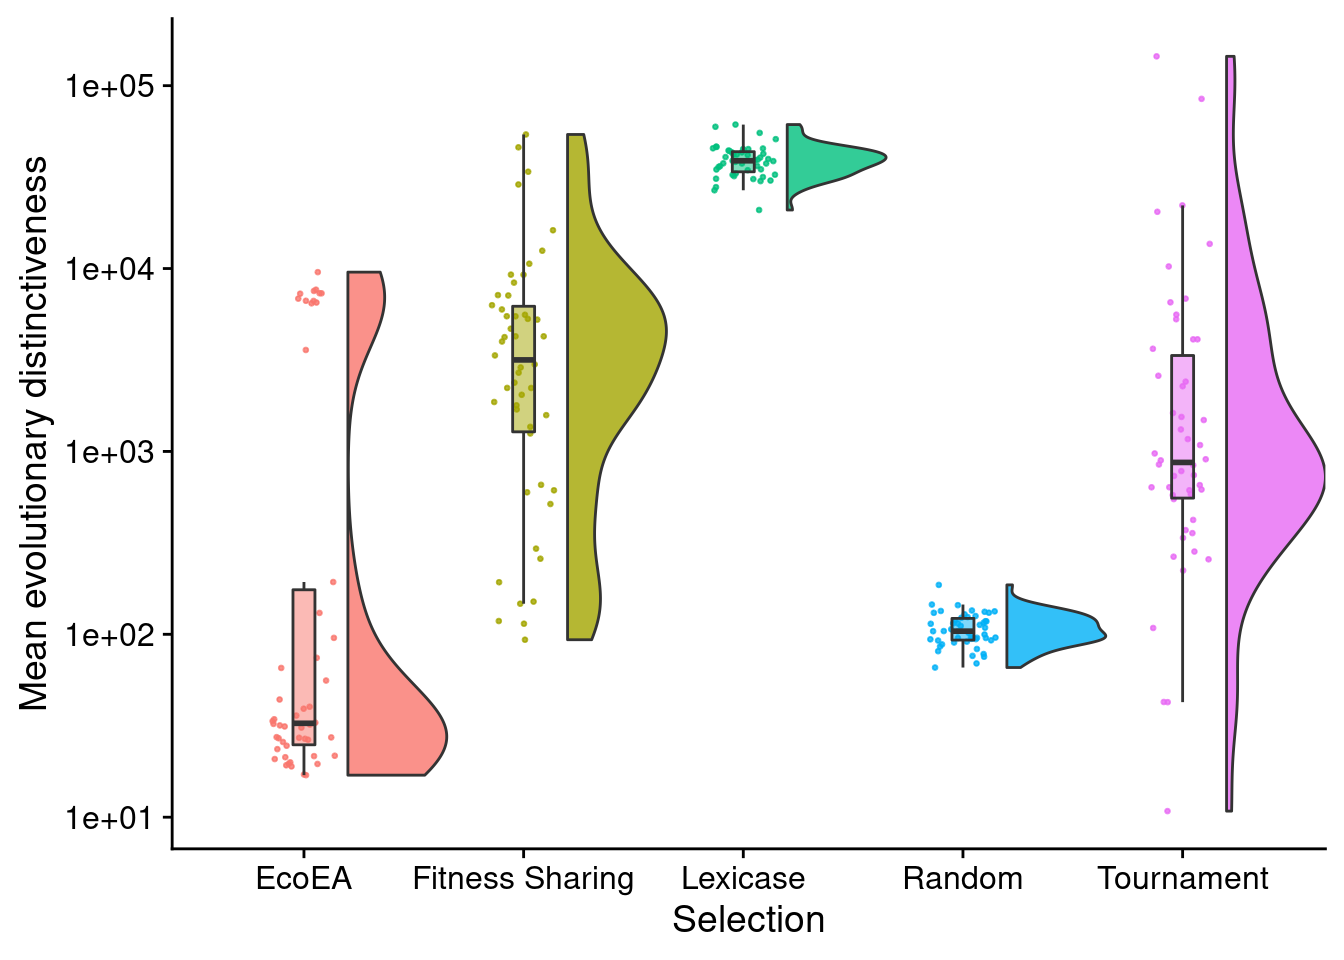
\includegraphics{phylodiversity-in-EC-supplement_files/figure-latex/final_phylogeny_plot_med-1.pdf}

\hypertarget{phenotypic-diversity}{%
\section{Phenotypic diversity}\label{phenotypic-diversity}}

\hypertarget{relationship-between-different-types-of-phenotypic-diversity}{%
\subsection{Relationship between different types of phenotypic diversity}\label{relationship-between-different-types-of-phenotypic-diversity}}

\begin{Shaded}
\begin{Highlighting}[]
\KeywordTok{ggplot}\NormalTok{(}
\NormalTok{    data }\OperatorTok\StringTok{ }\KeywordTok{filter}\NormalTok{(gen}\OperatorTok{==}\DecValTok{500000}\NormalTok{),}
    \KeywordTok{aes}\NormalTok{(}
        \DataTypeTok{y=}\NormalTok{phen_diversity,}
        \DataTypeTok{x=}\NormalTok{phen_num_taxa,}
        \DataTypeTok{color=}\NormalTok{selection_name,}
        \DataTypeTok{fill=}\NormalTok{selection_name}
\NormalTok{    )}
\NormalTok{  ) }\OperatorTok{+}
\StringTok{  }\KeywordTok{geom_point}\NormalTok{() }\OperatorTok{+}
\StringTok{    }\KeywordTok{scale_y_continuous}\NormalTok{(}
        \DataTypeTok{name=}\StringTok{"Phenotypic shannon diversity"}
\NormalTok{  ) }\OperatorTok{+}
\StringTok{  }\KeywordTok{scale_x_continuous}\NormalTok{(}
        \DataTypeTok{name=}\StringTok{"Phenotypic richness"}\NormalTok{,}
        \DataTypeTok{breaks =} \KeywordTok{breaks_extended}\NormalTok{(}\DecValTok{4}\NormalTok{)}
\NormalTok{  ) }\OperatorTok{+}\StringTok{ }
\StringTok{  }\KeywordTok{facet_wrap}\NormalTok{(}
      \OperatorTok{~}\NormalTok{selection_name, }\DataTypeTok{scales=}\StringTok{"free"}
\NormalTok{  ) }\OperatorTok{+}\StringTok{ }
\StringTok{  }\KeywordTok{stat_smooth}\NormalTok{(}
    \DataTypeTok{method=}\StringTok{"lm"}
\NormalTok{  ) }\OperatorTok{+}\StringTok{ }
\StringTok{  }\KeywordTok{stat_cor}\NormalTok{(}
    \DataTypeTok{method=}\StringTok{"spearman"}\NormalTok{, }\DataTypeTok{cor.coef.name =} \StringTok{"rho"}\NormalTok{, }\DataTypeTok{color=}\StringTok{"black"}
\NormalTok{  ) }\OperatorTok{+}
\StringTok{  }\KeywordTok{theme}\NormalTok{(}\DataTypeTok{legend.position =} \StringTok{"none"}\NormalTok{)}
\end{Highlighting}
\end{Shaded}

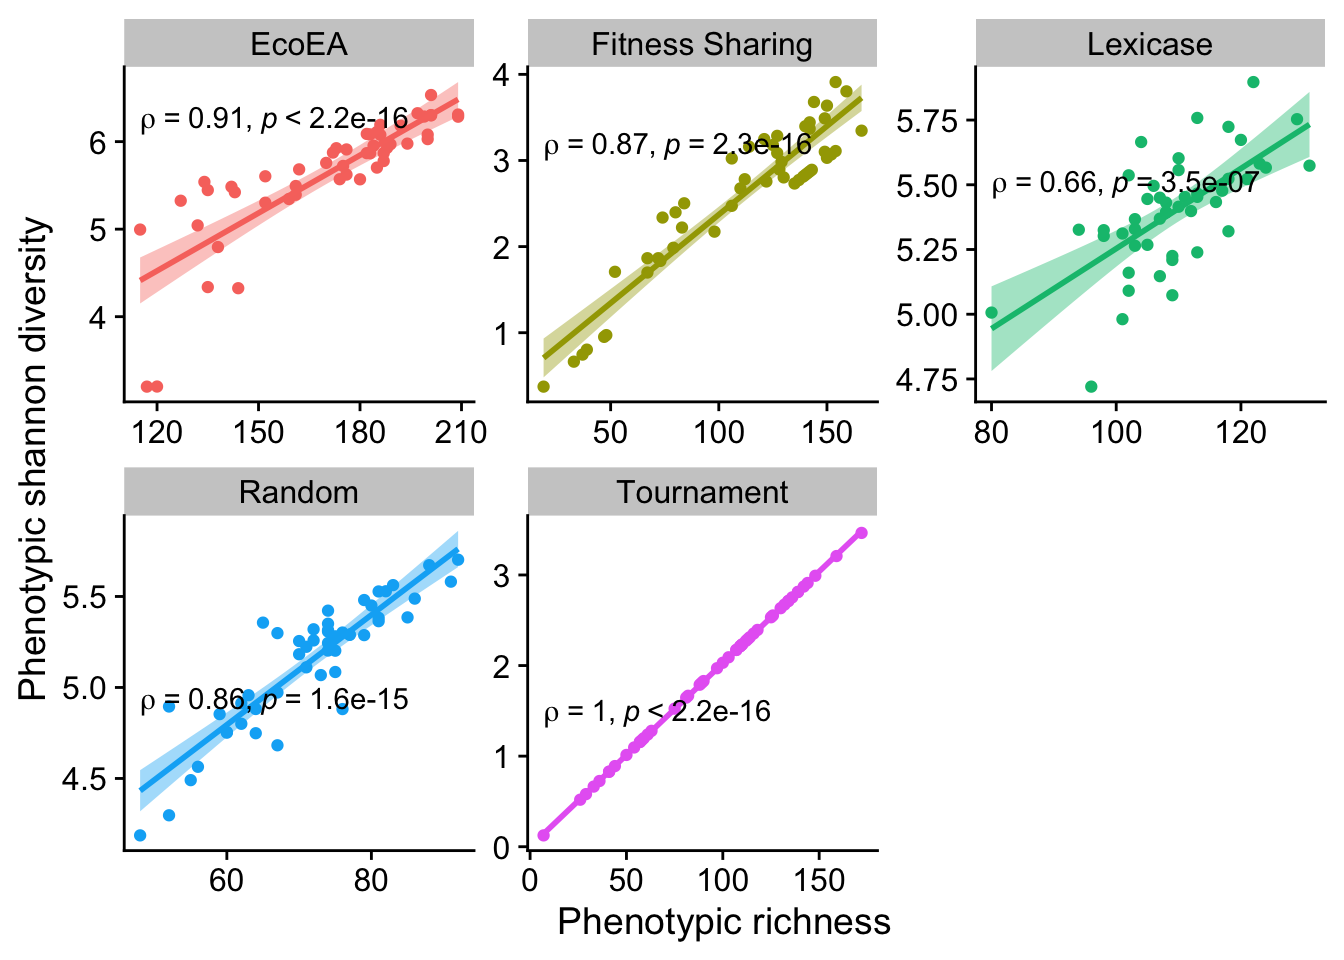
\includegraphics{phylodiversity-in-EC-supplement_files/figure-latex/richness_vs_shannon-1.pdf}

\hypertarget{over-time-2}{%
\subsection{Over time}\label{over-time-2}}

\begin{Shaded}
\begin{Highlighting}[]
\KeywordTok{ggplot}\NormalTok{(}
\NormalTok{    data,}
    \KeywordTok{aes}\NormalTok{(}
      \DataTypeTok{x=}\NormalTok{gen,}
      \DataTypeTok{y=}\NormalTok{phen_num_taxa,}
      \DataTypeTok{color=}\NormalTok{selection_name,}
      \DataTypeTok{fill=}\NormalTok{selection_name}
\NormalTok{    )}
\NormalTok{  ) }\OperatorTok{+}
\StringTok{  }\KeywordTok{stat_summary}\NormalTok{(}\DataTypeTok{geom=}\StringTok{"line"}\NormalTok{, }\DataTypeTok{fun=}\NormalTok{mean) }\OperatorTok{+}
\StringTok{  }\KeywordTok{stat_summary}\NormalTok{(}
    \DataTypeTok{geom=}\StringTok{"ribbon"}\NormalTok{,}
    \DataTypeTok{fun.data=}\StringTok{"mean_cl_boot"}\NormalTok{,}
    \DataTypeTok{fun.args=}\KeywordTok{list}\NormalTok{(}\DataTypeTok{conf.int=}\FloatTok{0.95}\NormalTok{),}
    \DataTypeTok{alpha=}\FloatTok{0.2}\NormalTok{,}
    \DataTypeTok{linetype=}\DecValTok{0}
\NormalTok{  ) }\OperatorTok{+}
\StringTok{  }\KeywordTok{scale_y_continuous}\NormalTok{(}
    \DataTypeTok{name=}\StringTok{"Phenotypic richness"}
\NormalTok{  ) }\OperatorTok{+}
\StringTok{  }\KeywordTok{scale_x_log10}\NormalTok{(}
    \DataTypeTok{name=}\StringTok{"Generation"}
\NormalTok{  ) }\OperatorTok{+}
\StringTok{  }\KeywordTok{scale_color_discrete}\NormalTok{(}\StringTok{"Selection"}\NormalTok{) }\OperatorTok{+}\StringTok{ }
\StringTok{  }\KeywordTok{scale_fill_discrete}\NormalTok{(}\StringTok{"Selection"}\NormalTok{)}
\end{Highlighting}
\end{Shaded}

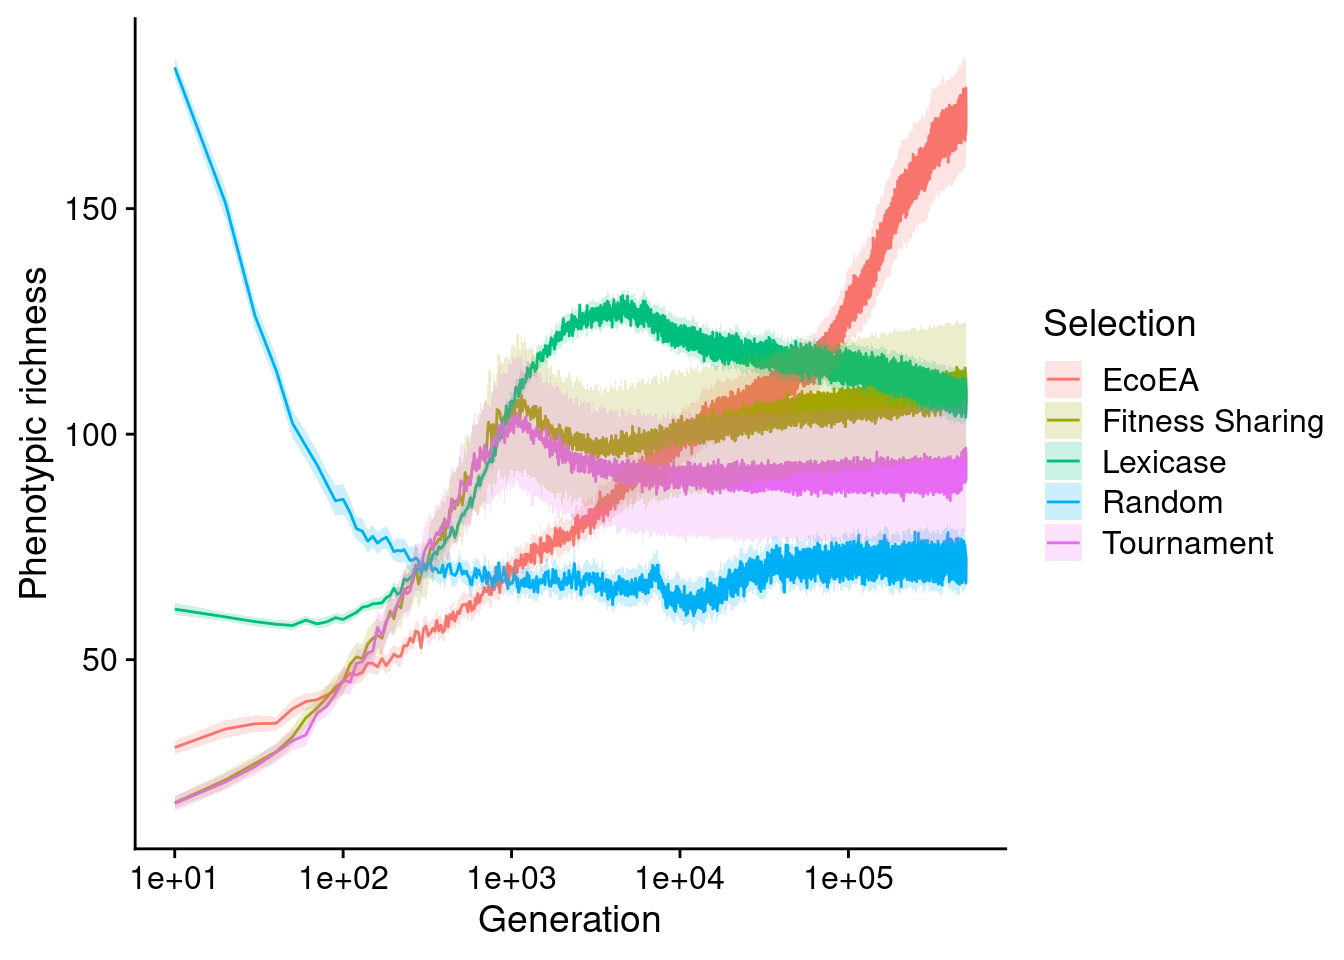
\includegraphics{phylodiversity-in-EC-supplement_files/figure-latex/phenotypic_diversity_over_time_plot-1.pdf}

In contrast to the phylodiversity results, phenotypic richness in all selection schemes (even tournament selection) ultimately exceeds that of random selection. Eco-EA monotonically increases while lexicase selection reaches a maximum around the same time it reaches its fitness plateau. The only real similarity to the phylodiversity results is the behavior tournament selection and fitness sharing relative to each other.

We also looked at phenotypic shannon entropy:

\begin{Shaded}
\begin{Highlighting}[]
\KeywordTok{ggplot}\NormalTok{(}
\NormalTok{    data,}
    \KeywordTok{aes}\NormalTok{(}
      \DataTypeTok{x=}\NormalTok{gen,}
      \DataTypeTok{y=}\NormalTok{phen_diversity,}
      \DataTypeTok{color=}\NormalTok{selection_name,}
      \DataTypeTok{fill=}\NormalTok{selection_name}
\NormalTok{    )}
\NormalTok{  ) }\OperatorTok{+}
\StringTok{  }\KeywordTok{stat_summary}\NormalTok{(}\DataTypeTok{geom=}\StringTok{"line"}\NormalTok{, }\DataTypeTok{fun=}\NormalTok{mean) }\OperatorTok{+}
\StringTok{  }\KeywordTok{stat_summary}\NormalTok{(}
    \DataTypeTok{geom=}\StringTok{"ribbon"}\NormalTok{,}
    \DataTypeTok{fun.data=}\StringTok{"mean_cl_boot"}\NormalTok{,}
    \DataTypeTok{fun.args=}\KeywordTok{list}\NormalTok{(}\DataTypeTok{conf.int=}\FloatTok{0.95}\NormalTok{),}
    \DataTypeTok{alpha=}\FloatTok{0.2}\NormalTok{,}
    \DataTypeTok{linetype=}\DecValTok{0}
\NormalTok{  ) }\OperatorTok{+}
\StringTok{  }\KeywordTok{scale_y_continuous}\NormalTok{(}
    \DataTypeTok{name=}\StringTok{"Phenotypic Shannon entropy"}
\NormalTok{  ) }\OperatorTok{+}
\StringTok{  }\KeywordTok{scale_x_log10}\NormalTok{(}
    \DataTypeTok{name=}\StringTok{"Generation"}
\NormalTok{  ) }\OperatorTok{+}
\StringTok{  }\KeywordTok{scale_color_discrete}\NormalTok{(}\StringTok{"Selection"}\NormalTok{) }\OperatorTok{+}\StringTok{ }
\StringTok{  }\KeywordTok{scale_fill_discrete}\NormalTok{(}\StringTok{"Selection"}\NormalTok{)}
\end{Highlighting}
\end{Shaded}

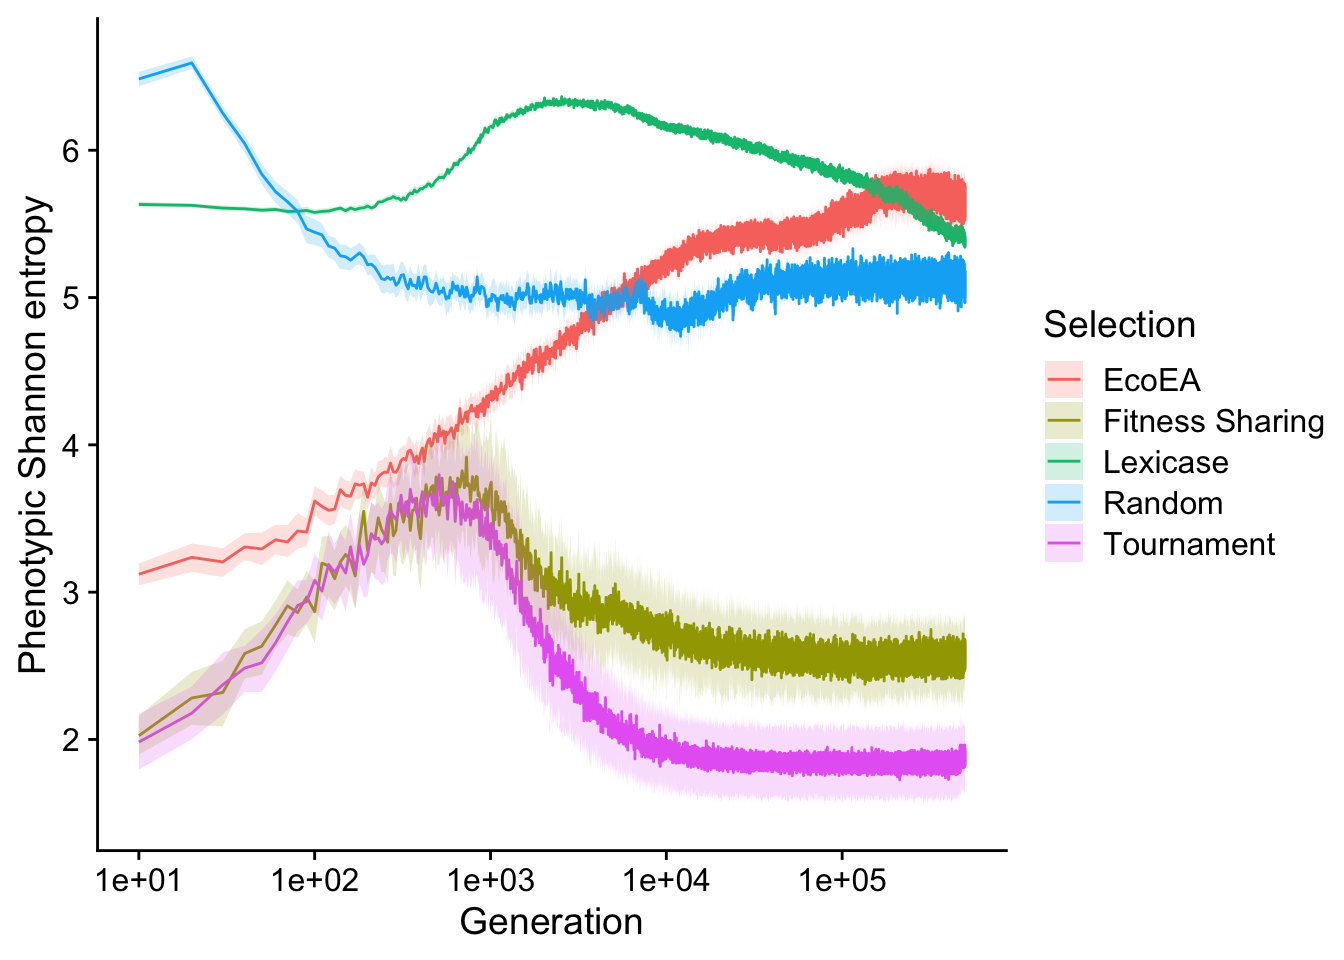
\includegraphics{phylodiversity-in-EC-supplement_files/figure-latex/phenotypic_diversity_over_time_plot_shannon-1.pdf}

\hypertarget{final-2}{%
\subsection{Final}\label{final-2}}

\hypertarget{richness}{%
\subsubsection{Richness}\label{richness}}

\begin{Shaded}
\begin{Highlighting}[]
\CommentTok{# Determine which conditions are significantly diferrent from each other}
\NormalTok{stat.test <-}\StringTok{ }\NormalTok{final_data }\OperatorTok
\StringTok{  }\KeywordTok{wilcox_test}\NormalTok{(phen_num_taxa }\OperatorTok{~}\StringTok{ }\NormalTok{selection_name) }\OperatorTok
\StringTok{  }\KeywordTok{adjust_pvalue}\NormalTok{(}\DataTypeTok{method =} \StringTok{"bonferroni"}\NormalTok{) }\OperatorTok
\StringTok{  }\KeywordTok{add_significance}\NormalTok{() }\OperatorTok
\StringTok{  }\KeywordTok{add_xy_position}\NormalTok{(}\DataTypeTok{x=}\StringTok{"selection_name"}\NormalTok{,}\DataTypeTok{step.increase=}\DecValTok{1}\NormalTok{)}
\NormalTok{stat.test}\OperatorTok{$}\NormalTok{label <-}\StringTok{ }\KeywordTok{mapply}\NormalTok{(p_label,stat.test}\OperatorTok{$}\NormalTok{p.adj)}

\NormalTok{stat.test }\OperatorTok
\StringTok{  }\KeywordTok{kbl}\NormalTok{() }\OperatorTok
\StringTok{  }\KeywordTok{kable_styling}\NormalTok{(}
    \DataTypeTok{bootstrap_options =} \KeywordTok{c}\NormalTok{(}
      \StringTok{"striped"}\NormalTok{,}
      \StringTok{"hover"}\NormalTok{,}
      \StringTok{"condensed"}\NormalTok{,}
      \StringTok{"responsive"}
\NormalTok{    )}
\NormalTok{  ) }\OperatorTok
\StringTok{  }\KeywordTok{scroll_box}\NormalTok{(}\DataTypeTok{width=}\StringTok{"600px"}\NormalTok{)}
\end{Highlighting}
\end{Shaded}

\begin{table}
\centering
\begin{tabular}[t]{l|l|l|r|r|r|r|r|l|r|l|r|r|l}
\hline
.y. & group1 & group2 & n1 & n2 & statistic & p & p.adj & p.adj.signif & y.position & groups & xmin & xmax & label\\
\hline
phen\_num\_taxa & EcoEA & Fitness Sharing & 50 & 50 & 2249.0 & 0.00e+00 & 0.0e+00 & **** & 326 & EcoEA          , Fitness Sharing & 1 & 2 & p < 1e-04\\
\hline
phen\_num\_taxa & EcoEA & Lexicase & 50 & 47 & 2319.0 & 0.00e+00 & 0.0e+00 & **** & 456 & EcoEA   , Lexicase & 1 & 3 & p < 1e-04\\
\hline
phen\_num\_taxa & EcoEA & Random & 50 & 50 & 2500.0 & 0.00e+00 & 0.0e+00 & **** & 586 & EcoEA , Random & 1 & 4 & p < 1e-04\\
\hline
phen\_num\_taxa & EcoEA & Tournament & 50 & 50 & 2378.5 & 0.00e+00 & 0.0e+00 & **** & 716 & EcoEA     , Tournament & 1 & 5 & p < 1e-04\\
\hline
phen\_num\_taxa & Fitness Sharing & Lexicase & 50 & 47 & 1428.0 & 6.80e-02 & 6.8e-01 & ns & 846 & Fitness Sharing, Lexicase & 2 & 3 & p = 0.68\\
\hline
phen\_num\_taxa & Fitness Sharing & Random & 50 & 50 & 1973.0 & 6.00e-07 & 6.3e-06 & **** & 976 & Fitness Sharing, Random & 2 & 4 & p < 1e-04\\
\hline
phen\_num\_taxa & Fitness Sharing & Tournament & 50 & 50 & 1585.0 & 2.10e-02 & 2.1e-01 & ns & 1106 & Fitness Sharing, Tournament & 2 & 5 & p = 0.21\\
\hline
phen\_num\_taxa & Lexicase & Random & 47 & 50 & 2339.5 & 0.00e+00 & 0.0e+00 & **** & 1236 & Lexicase, Random & 3 & 4 & p < 1e-04\\
\hline
phen\_num\_taxa & Lexicase & Tournament & 47 & 50 & 1359.0 & 1.85e-01 & 1.0e+00 & ns & 1366 & Lexicase  , Tournament & 3 & 5 & p = 1\\
\hline
phen\_num\_taxa & Random & Tournament & 50 & 50 & 797.0 & 2.00e-03 & 2.0e-02 & * & 1496 & Random    , Tournament & 4 & 5 & p = 0.02\\
\hline
\end{tabular}
\end{table}

\begin{Shaded}
\begin{Highlighting}[]
\CommentTok{# Raincloud plot of final phenotypic diversity}
\NormalTok{final_phenotypic_fig <-}\StringTok{ }\KeywordTok{ggplot}\NormalTok{(}
\NormalTok{    final_data,}
    \KeywordTok{aes}\NormalTok{(}
      \DataTypeTok{x=}\NormalTok{selection_name,}
      \DataTypeTok{y=}\NormalTok{phen_num_taxa,}
      \DataTypeTok{fill=}\NormalTok{selection_name}
\NormalTok{    )}
\NormalTok{  ) }\OperatorTok{+}
\StringTok{  }\KeywordTok{geom_flat_violin}\NormalTok{(}
    \DataTypeTok{position =} \KeywordTok{position_nudge}\NormalTok{(}\DataTypeTok{x =} \FloatTok{.2}\NormalTok{, }\DataTypeTok{y =} \DecValTok{0}\NormalTok{),}
    \DataTypeTok{alpha =} \FloatTok{.8}\NormalTok{,}
    \DataTypeTok{scale=}\StringTok{"width"}
\NormalTok{  ) }\OperatorTok{+}
\StringTok{  }\KeywordTok{geom_point}\NormalTok{(}
    \DataTypeTok{mapping=}\KeywordTok{aes}\NormalTok{(}\DataTypeTok{color=}\NormalTok{selection_name),}
    \DataTypeTok{position =} \KeywordTok{position_jitter}\NormalTok{(}\DataTypeTok{width =} \FloatTok{.15}\NormalTok{),}
    \DataTypeTok{size =} \FloatTok{.5}\NormalTok{,}
    \DataTypeTok{alpha =} \FloatTok{0.8}
\NormalTok{  ) }\OperatorTok{+}
\StringTok{  }\KeywordTok{geom_boxplot}\NormalTok{(}
    \DataTypeTok{width =} \FloatTok{.1}\NormalTok{,}
    \DataTypeTok{outlier.shape =} \OtherTok{NA}\NormalTok{,}
    \DataTypeTok{alpha =} \FloatTok{0.5}
\NormalTok{  ) }\OperatorTok{+}
\StringTok{  }\KeywordTok{scale_y_continuous}\NormalTok{(}
    \DataTypeTok{name=}\StringTok{"Phenotypic Richness"}
\NormalTok{  ) }\OperatorTok{+}
\StringTok{  }\KeywordTok{scale_x_discrete}\NormalTok{(}
    \DataTypeTok{name=}\StringTok{"Selection"}
\NormalTok{  ) }\OperatorTok{+}
\StringTok{  }\KeywordTok{scale_fill_discrete}\NormalTok{(}
    \DataTypeTok{name=}\StringTok{"Selection"}
\NormalTok{  ) }\OperatorTok{+}
\StringTok{  }\KeywordTok{scale_color_discrete}\NormalTok{(}
    \DataTypeTok{name=}\StringTok{"Selection"}
\NormalTok{  ) }\OperatorTok{+}
\StringTok{  }\KeywordTok{theme}\NormalTok{(}\DataTypeTok{legend.position =} \StringTok{"none"}\NormalTok{)}
\NormalTok{final_phenotypic_fig}
\end{Highlighting}
\end{Shaded}

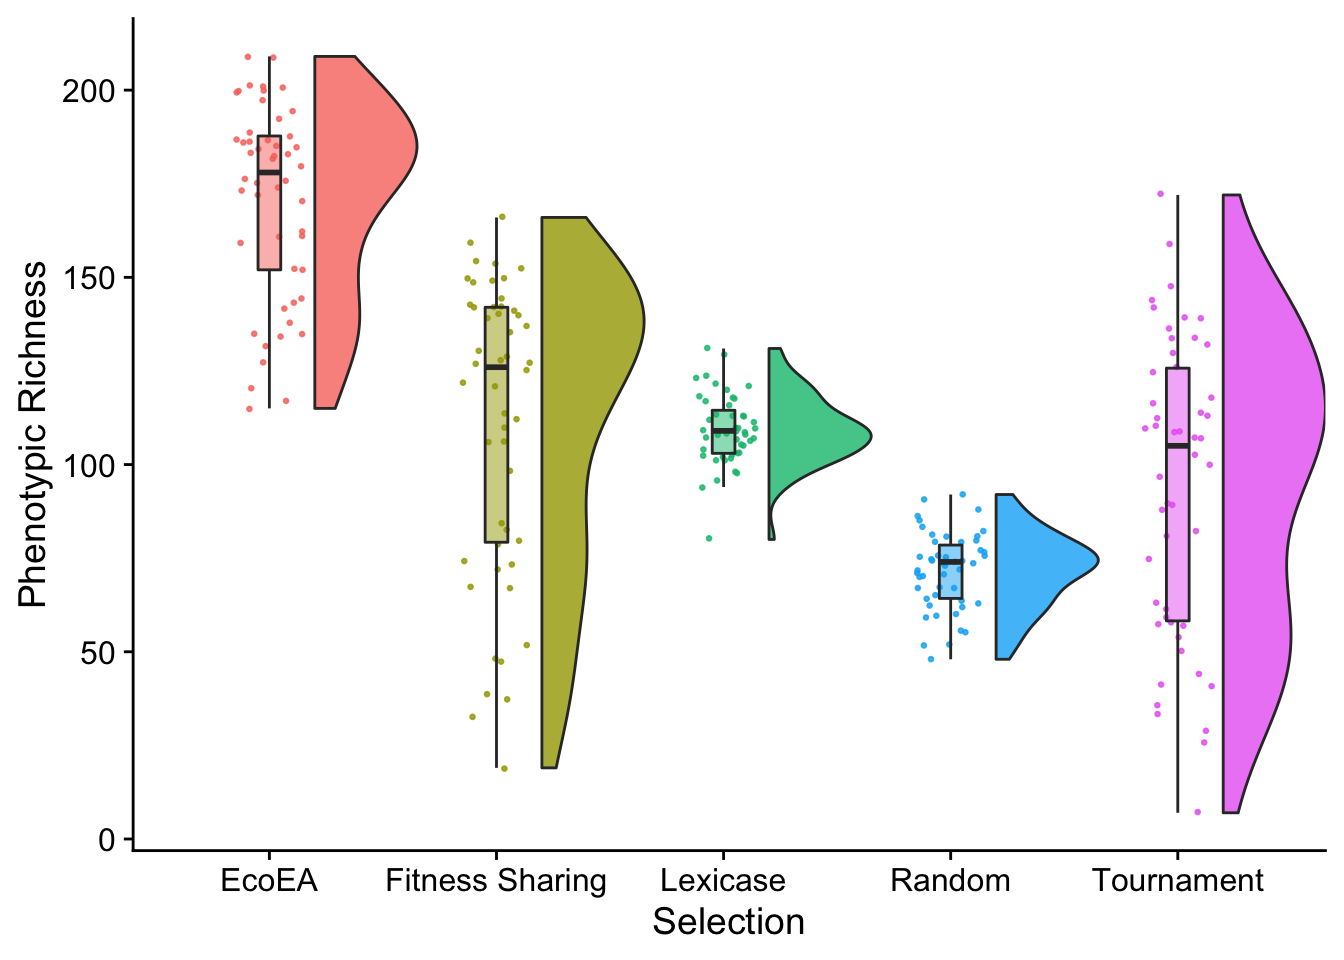
\includegraphics{phylodiversity-in-EC-supplement_files/figure-latex/final_phenotypic_plot-1.pdf}

Nothing particularly suprising here, but we should note that, based on the over time plot, this would look a lot different if we had selected a different time point.

\hypertarget{shannon-diversity}{%
\subsubsection{Shannon diversity}\label{shannon-diversity}}

\begin{Shaded}
\begin{Highlighting}[]
\CommentTok{# Determine which conditions are significantly diferrent from each other}
\NormalTok{stat.test <-}\StringTok{ }\NormalTok{final_data }\OperatorTok
\StringTok{  }\KeywordTok{wilcox_test}\NormalTok{(phen_diversity}\OperatorTok{~}\StringTok{ }\NormalTok{selection_name) }\OperatorTok
\StringTok{  }\KeywordTok{adjust_pvalue}\NormalTok{(}\DataTypeTok{method =} \StringTok{"bonferroni"}\NormalTok{) }\OperatorTok
\StringTok{  }\KeywordTok{add_significance}\NormalTok{() }\OperatorTok
\StringTok{  }\KeywordTok{add_xy_position}\NormalTok{(}\DataTypeTok{x=}\StringTok{"selection_name"}\NormalTok{,}\DataTypeTok{step.increase=}\DecValTok{1}\NormalTok{)}
\NormalTok{stat.test}\OperatorTok{$}\NormalTok{label <-}\StringTok{ }\KeywordTok{mapply}\NormalTok{(p_label,stat.test}\OperatorTok{$}\NormalTok{p.adj)}

\NormalTok{stat.test }\OperatorTok
\StringTok{  }\KeywordTok{kbl}\NormalTok{() }\OperatorTok
\StringTok{  }\KeywordTok{kable_styling}\NormalTok{(}
    \DataTypeTok{bootstrap_options =} \KeywordTok{c}\NormalTok{(}
      \StringTok{"striped"}\NormalTok{,}
      \StringTok{"hover"}\NormalTok{,}
      \StringTok{"condensed"}\NormalTok{,}
      \StringTok{"responsive"}
\NormalTok{    )}
\NormalTok{  ) }\OperatorTok
\StringTok{  }\KeywordTok{scroll_box}\NormalTok{(}\DataTypeTok{width=}\StringTok{"600px"}\NormalTok{)}
\end{Highlighting}
\end{Shaded}

\begin{table}
\centering
\begin{tabular}[t]{l|l|l|r|r|r|r|r|l|r|l|r|r|l}
\hline
.y. & group1 & group2 & n1 & n2 & statistic & p & p.adj & p.adj.signif & y.position & groups & xmin & xmax & label\\
\hline
phen\_diversity & EcoEA & Fitness Sharing & 50 & 50 & 2478.0 & 0.00e+00 & 0.00e+00 & **** & 9.602 & EcoEA          , Fitness Sharing & 1 & 2 & p < 1e-04\\
\hline
phen\_diversity & EcoEA & Lexicase & 50 & 47 & 1772.0 & 1.66e-05 & 1.66e-04 & *** & 13.012 & EcoEA   , Lexicase & 1 & 3 & p = 0.000166\\
\hline
phen\_diversity & EcoEA & Random & 50 & 50 & 2089.5 & 0.00e+00 & 1.00e-07 & **** & 16.422 & EcoEA , Random & 1 & 4 & p < 1e-04\\
\hline
phen\_diversity & EcoEA & Tournament & 50 & 50 & 2496.0 & 0.00e+00 & 0.00e+00 & **** & 19.832 & EcoEA     , Tournament & 1 & 5 & p < 1e-04\\
\hline
phen\_diversity & Fitness Sharing & Lexicase & 50 & 47 & 0.0 & 0.00e+00 & 0.00e+00 & **** & 23.242 & Fitness Sharing, Lexicase & 2 & 3 & p < 1e-04\\
\hline
phen\_diversity & Fitness Sharing & Random & 50 & 50 & 0.0 & 0.00e+00 & 0.00e+00 & **** & 26.652 & Fitness Sharing, Random & 2 & 4 & p < 1e-04\\
\hline
phen\_diversity & Fitness Sharing & Tournament & 50 & 50 & 1856.0 & 2.99e-05 & 2.99e-04 & *** & 30.062 & Fitness Sharing, Tournament & 2 & 5 & p = 0.000299\\
\hline
phen\_diversity & Lexicase & Random & 47 & 50 & 1714.0 & 1.01e-04 & 1.01e-03 & ** & 33.472 & Lexicase, Random & 3 & 4 & p = 0.00101\\
\hline
phen\_diversity & Lexicase & Tournament & 47 & 50 & 2350.0 & 0.00e+00 & 0.00e+00 & **** & 36.882 & Lexicase  , Tournament & 3 & 5 & p < 1e-04\\
\hline
phen\_diversity & Random & Tournament & 50 & 50 & 2500.0 & 0.00e+00 & 0.00e+00 & **** & 40.292 & Random    , Tournament & 4 & 5 & p < 1e-04\\
\hline
\end{tabular}
\end{table}

\begin{Shaded}
\begin{Highlighting}[]
\CommentTok{# Raincloud plot of final phenotypic diversity}
\KeywordTok{ggplot}\NormalTok{(}
\NormalTok{    final_data,}
    \KeywordTok{aes}\NormalTok{(}
      \DataTypeTok{x=}\NormalTok{selection_name,}
      \DataTypeTok{y=}\NormalTok{phen_num_taxa,}
      \DataTypeTok{fill=}\NormalTok{selection_name}
\NormalTok{    )}
\NormalTok{  ) }\OperatorTok{+}
\StringTok{  }\KeywordTok{geom_flat_violin}\NormalTok{(}
    \DataTypeTok{position =} \KeywordTok{position_nudge}\NormalTok{(}\DataTypeTok{x =} \FloatTok{.2}\NormalTok{, }\DataTypeTok{y =} \DecValTok{0}\NormalTok{),}
    \DataTypeTok{alpha =} \FloatTok{.8}\NormalTok{,}
    \DataTypeTok{scale=}\StringTok{"width"}
\NormalTok{  ) }\OperatorTok{+}
\StringTok{  }\KeywordTok{geom_point}\NormalTok{(}
    \DataTypeTok{mapping=}\KeywordTok{aes}\NormalTok{(}\DataTypeTok{color=}\NormalTok{selection_name),}
    \DataTypeTok{position =} \KeywordTok{position_jitter}\NormalTok{(}\DataTypeTok{width =} \FloatTok{.15}\NormalTok{),}
    \DataTypeTok{size =} \FloatTok{.5}\NormalTok{,}
    \DataTypeTok{alpha =} \FloatTok{0.8}
\NormalTok{  ) }\OperatorTok{+}
\StringTok{  }\KeywordTok{geom_boxplot}\NormalTok{(}
    \DataTypeTok{width =} \FloatTok{.1}\NormalTok{,}
    \DataTypeTok{outlier.shape =} \OtherTok{NA}\NormalTok{,}
    \DataTypeTok{alpha =} \FloatTok{0.5}
\NormalTok{  ) }\OperatorTok{+}
\StringTok{  }\KeywordTok{scale_y_continuous}\NormalTok{(}
    \DataTypeTok{name=}\StringTok{"Phenotypic Shannon Diversity"}
\NormalTok{  ) }\OperatorTok{+}
\StringTok{  }\KeywordTok{scale_x_discrete}\NormalTok{(}
    \DataTypeTok{name=}\StringTok{"Selection"}
\NormalTok{  ) }\OperatorTok{+}
\StringTok{  }\KeywordTok{scale_fill_discrete}\NormalTok{(}
    \DataTypeTok{name=}\StringTok{"Selection"}
\NormalTok{  ) }\OperatorTok{+}
\StringTok{  }\KeywordTok{scale_color_discrete}\NormalTok{(}
    \DataTypeTok{name=}\StringTok{"Selection"}
\NormalTok{  ) }\OperatorTok{+}
\StringTok{  }\KeywordTok{theme}\NormalTok{(}\DataTypeTok{legend.position =} \StringTok{"none"}\NormalTok{)}
\end{Highlighting}
\end{Shaded}

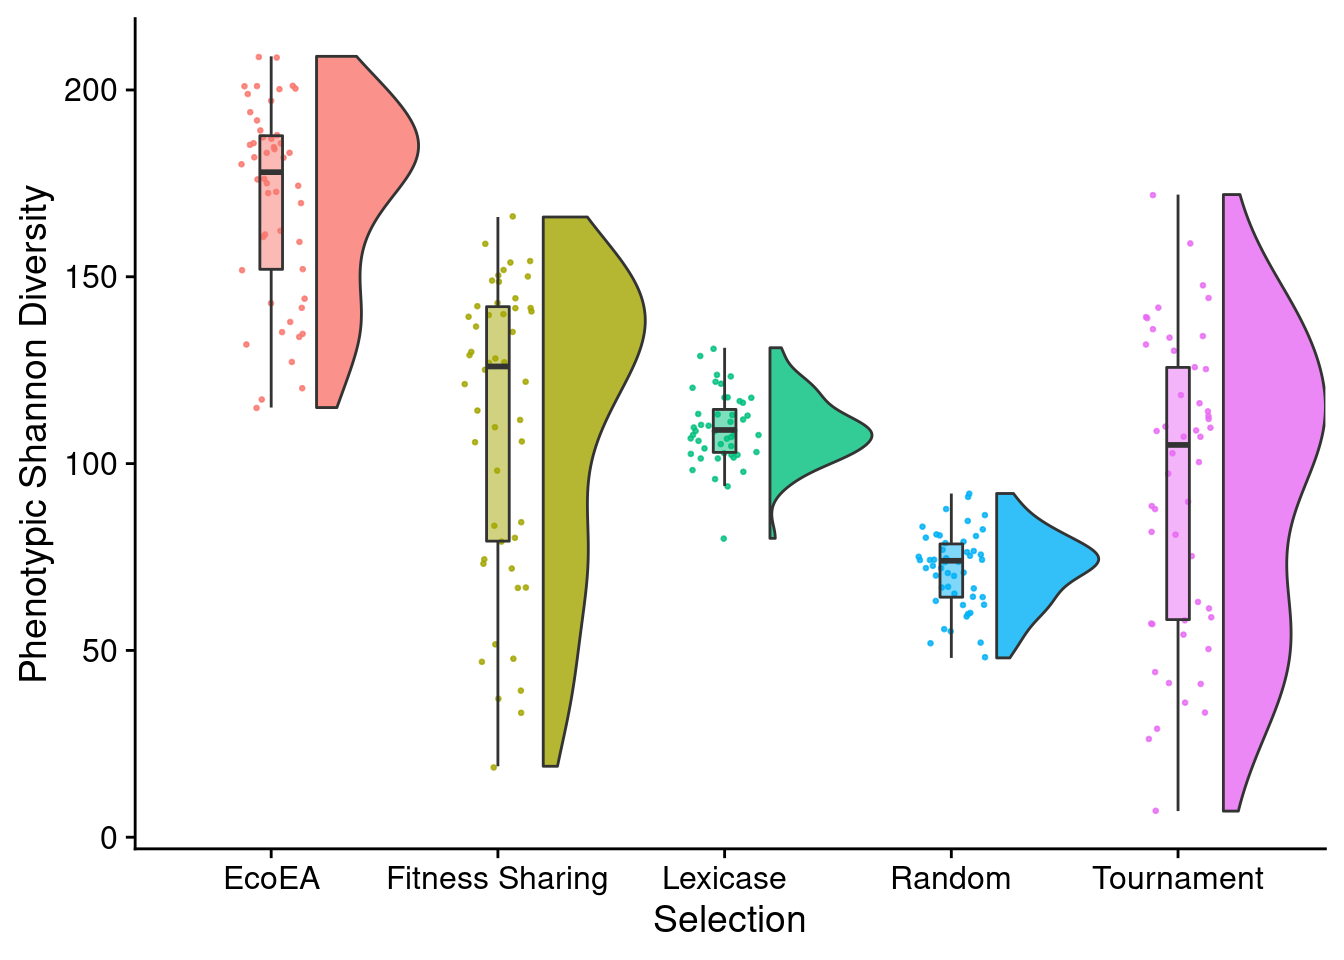
\includegraphics{phylodiversity-in-EC-supplement_files/figure-latex/final_phenotypic_plot_shannon-1.pdf}

\hypertarget{relationship-between-phenotypic-and-phylogenetic-diversity}{%
\section{Relationship between phenotypic and phylogenetic diversity}\label{relationship-between-phenotypic-and-phylogenetic-diversity}}

\begin{Shaded}
\begin{Highlighting}[]
\KeywordTok{ggplot}\NormalTok{(}
\NormalTok{    data }\OperatorTok\StringTok{ }\KeywordTok{filter}\NormalTok{(gen}\OperatorTok{==}\DecValTok{500000}\NormalTok{),}
    \KeywordTok{aes}\NormalTok{(}
        \DataTypeTok{y=}\NormalTok{phen_num_taxa,}
        \DataTypeTok{x=}\NormalTok{mean_phenotype_pairwise_distance,}
        \DataTypeTok{color=}\NormalTok{selection_name,}
        \DataTypeTok{fill=}\NormalTok{selection_name}
\NormalTok{    )}
\NormalTok{  ) }\OperatorTok{+}
\StringTok{  }\KeywordTok{geom_point}\NormalTok{() }\OperatorTok{+}
\StringTok{    }\KeywordTok{scale_y_continuous}\NormalTok{(}
        \DataTypeTok{name=}\StringTok{"Phenotypic richness"}
\NormalTok{  ) }\OperatorTok{+}
\StringTok{  }\KeywordTok{scale_x_continuous}\NormalTok{(}
        \DataTypeTok{name=}\StringTok{"Mean pairwise distance"}\NormalTok{,}
        \DataTypeTok{breaks =} \KeywordTok{breaks_extended}\NormalTok{(}\DecValTok{4}\NormalTok{)}
\NormalTok{  ) }\OperatorTok{+}\StringTok{ }
\StringTok{  }\KeywordTok{facet_wrap}\NormalTok{(}
      \OperatorTok{~}\NormalTok{selection_name, }\DataTypeTok{scales=}\StringTok{"free"}
\NormalTok{  ) }\OperatorTok{+}\StringTok{ }
\StringTok{  }\KeywordTok{stat_smooth}\NormalTok{(}
    \DataTypeTok{method=}\StringTok{"lm"}
\NormalTok{  ) }\OperatorTok{+}\StringTok{ }
\StringTok{  }\KeywordTok{stat_cor}\NormalTok{(}
    \DataTypeTok{method=}\StringTok{"spearman"}\NormalTok{, }\DataTypeTok{cor.coef.name =} \StringTok{"rho"}\NormalTok{, }\DataTypeTok{color=}\StringTok{"black"}
\NormalTok{  ) }\OperatorTok{+}
\StringTok{  }\KeywordTok{theme}\NormalTok{(}\DataTypeTok{legend.position =} \StringTok{"none"}\NormalTok{)}
\end{Highlighting}
\end{Shaded}

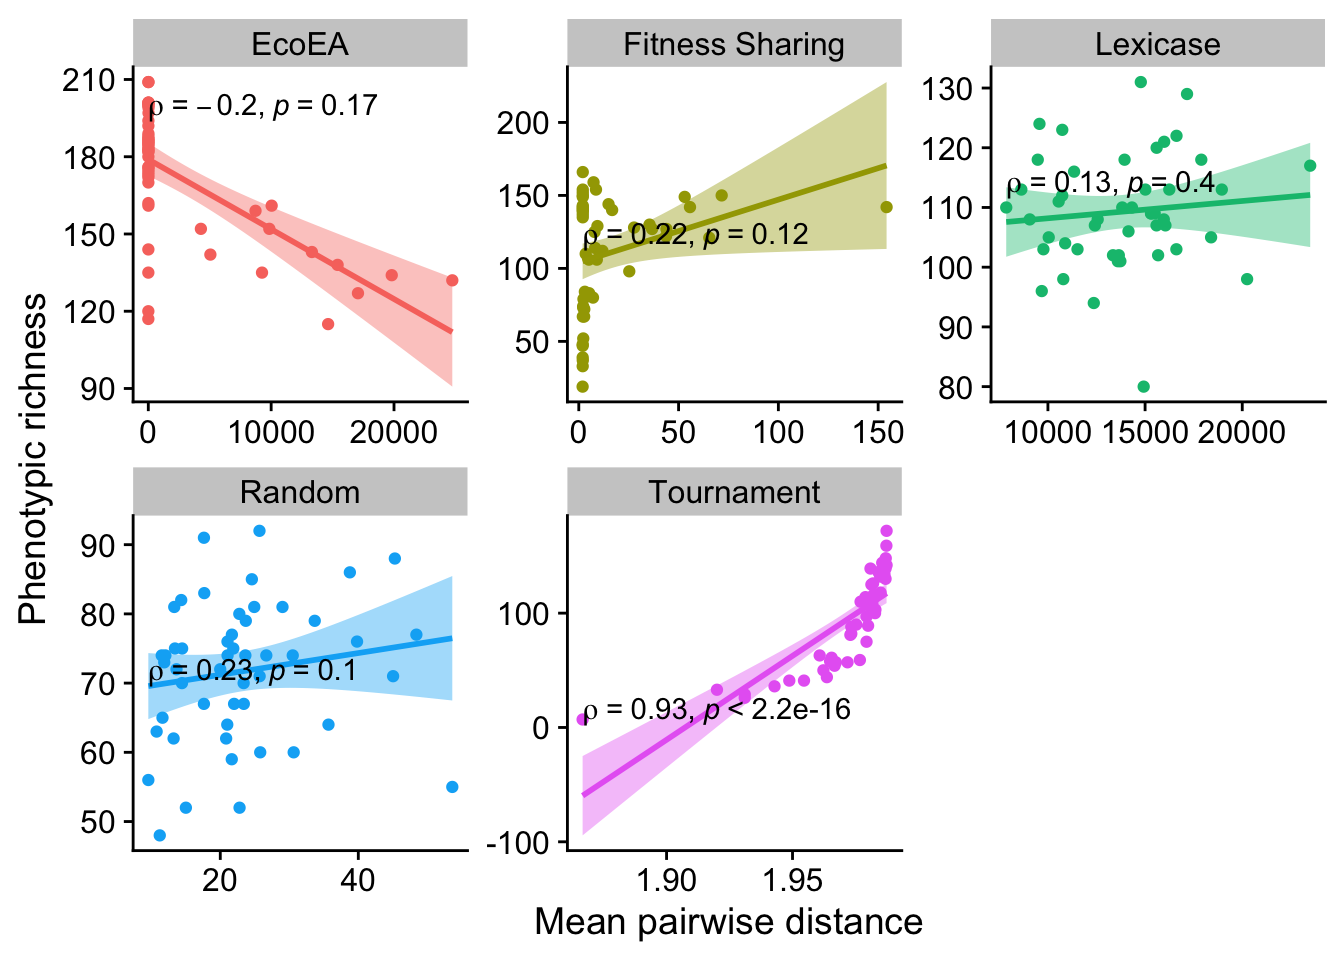
\includegraphics{phylodiversity-in-EC-supplement_files/figure-latex/phen_vs_phylo_richness_mpd-1.pdf}

\begin{Shaded}
\begin{Highlighting}[]
\KeywordTok{ggplot}\NormalTok{(}
\NormalTok{    data }\OperatorTok\StringTok{ }\KeywordTok{filter}\NormalTok{(gen}\OperatorTok{==}\DecValTok{500000}\NormalTok{),}
    \KeywordTok{aes}\NormalTok{(}
        \DataTypeTok{y=}\NormalTok{phen_num_taxa,}
        \DataTypeTok{x=}\NormalTok{mean_phenotype_evolutionary_distinctiveness,}
        \DataTypeTok{color=}\NormalTok{selection_name,}
        \DataTypeTok{fill=}\NormalTok{selection_name}
\NormalTok{    )}
\NormalTok{  ) }\OperatorTok{+}
\StringTok{  }\KeywordTok{geom_point}\NormalTok{() }\OperatorTok{+}
\StringTok{    }\KeywordTok{scale_y_continuous}\NormalTok{(}
        \DataTypeTok{name=}\StringTok{"Phenotypic richness"}
\NormalTok{  ) }\OperatorTok{+}
\StringTok{  }\KeywordTok{scale_x_continuous}\NormalTok{(}
        \DataTypeTok{name=}\StringTok{"Mean evolutionary distinctiveness"}\NormalTok{,}
        \DataTypeTok{breaks =} \KeywordTok{breaks_extended}\NormalTok{(}\DecValTok{4}\NormalTok{)}
\NormalTok{  ) }\OperatorTok{+}\StringTok{ }
\StringTok{  }\KeywordTok{facet_wrap}\NormalTok{(}
      \OperatorTok{~}\NormalTok{selection_name, }\DataTypeTok{scales=}\StringTok{"free"}
\NormalTok{  ) }\OperatorTok{+}\StringTok{ }
\StringTok{  }\KeywordTok{stat_smooth}\NormalTok{(}
    \DataTypeTok{method=}\StringTok{"lm"}
\NormalTok{  ) }\OperatorTok{+}\StringTok{ }
\StringTok{  }\KeywordTok{stat_cor}\NormalTok{(}
    \DataTypeTok{method=}\StringTok{"spearman"}\NormalTok{, }\DataTypeTok{cor.coef.name =} \StringTok{"rho"}\NormalTok{, }\DataTypeTok{color=}\StringTok{"black"}
\NormalTok{  ) }\OperatorTok{+}
\StringTok{  }\KeywordTok{theme}\NormalTok{(}\DataTypeTok{legend.position =} \StringTok{"none"}\NormalTok{)}
\end{Highlighting}
\end{Shaded}

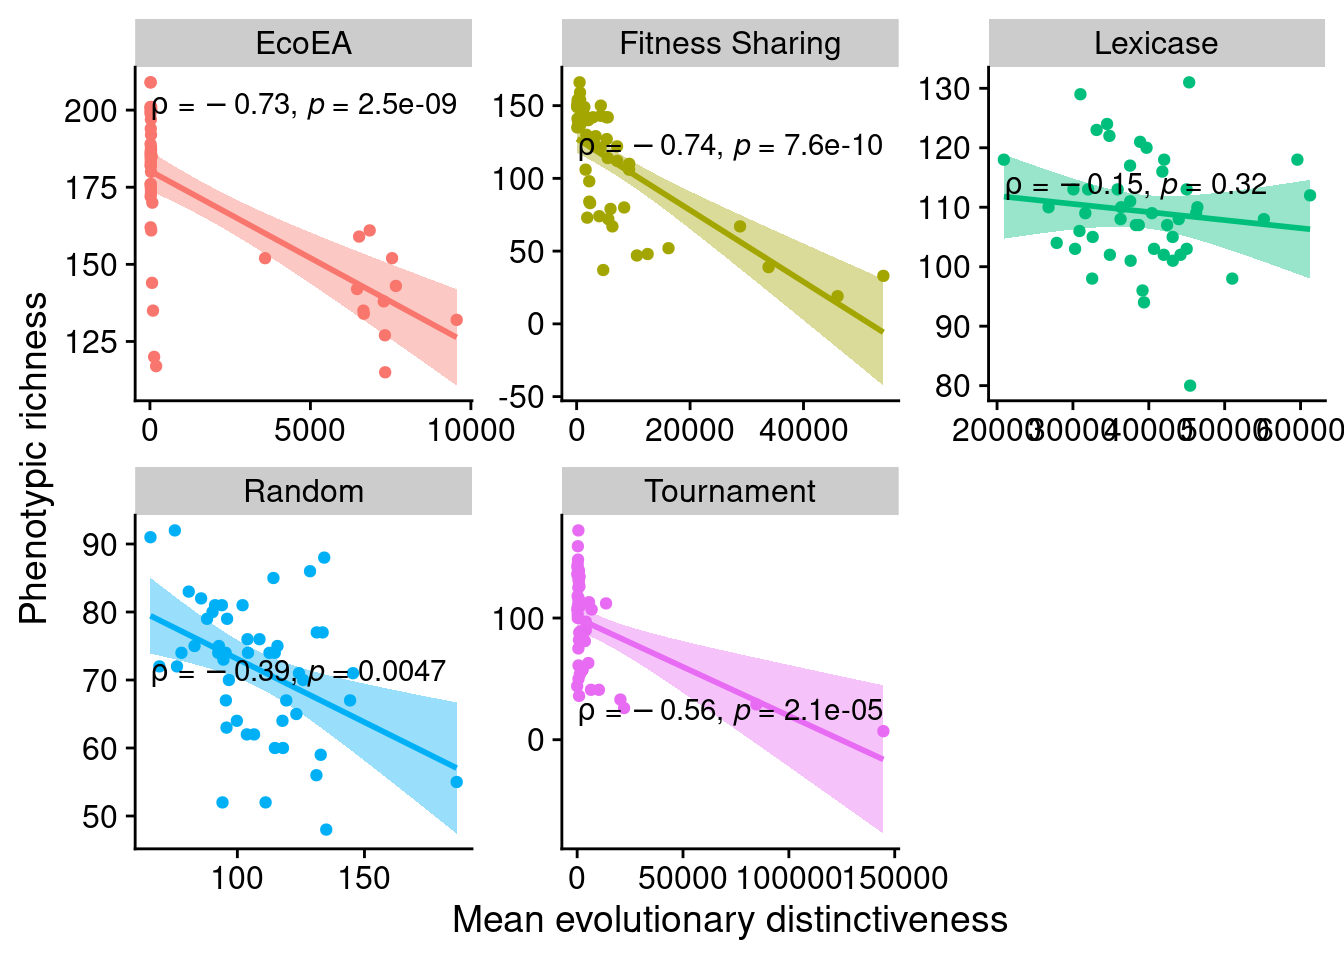
\includegraphics{phylodiversity-in-EC-supplement_files/figure-latex/phen_vs_phylo_richness_med-1.pdf}

\begin{Shaded}
\begin{Highlighting}[]
\KeywordTok{ggplot}\NormalTok{(}
\NormalTok{    data }\OperatorTok\StringTok{ }\KeywordTok{filter}\NormalTok{(gen}\OperatorTok{==}\DecValTok{500000}\NormalTok{),}
    \KeywordTok{aes}\NormalTok{(}
        \DataTypeTok{y=}\NormalTok{phen_diversity,}
        \DataTypeTok{x=}\NormalTok{mean_phenotype_pairwise_distance,}
        \DataTypeTok{color=}\NormalTok{selection_name,}
        \DataTypeTok{fill=}\NormalTok{selection_name}
\NormalTok{    )}
\NormalTok{  ) }\OperatorTok{+}
\StringTok{  }\KeywordTok{geom_point}\NormalTok{() }\OperatorTok{+}
\StringTok{    }\KeywordTok{scale_y_continuous}\NormalTok{(}
        \DataTypeTok{name=}\StringTok{"Phenotypic shannon diversity"}
\NormalTok{  ) }\OperatorTok{+}
\StringTok{  }\KeywordTok{scale_x_continuous}\NormalTok{(}
        \DataTypeTok{name=}\StringTok{"Mean pairwise distance"}\NormalTok{,}
        \DataTypeTok{breaks =} \KeywordTok{breaks_extended}\NormalTok{(}\DecValTok{4}\NormalTok{)}
\NormalTok{  ) }\OperatorTok{+}\StringTok{ }
\StringTok{  }\KeywordTok{facet_wrap}\NormalTok{(}
      \OperatorTok{~}\NormalTok{selection_name, }\DataTypeTok{scales=}\StringTok{"free"}
\NormalTok{  ) }\OperatorTok{+}\StringTok{ }
\StringTok{  }\KeywordTok{stat_smooth}\NormalTok{(}
    \DataTypeTok{method=}\StringTok{"lm"}
\NormalTok{  ) }\OperatorTok{+}\StringTok{ }
\StringTok{  }\KeywordTok{stat_cor}\NormalTok{(}
    \DataTypeTok{method=}\StringTok{"spearman"}\NormalTok{, }\DataTypeTok{cor.coef.name =} \StringTok{"rho"}\NormalTok{, }\DataTypeTok{color=}\StringTok{"black"}
\NormalTok{  ) }\OperatorTok{+}
\StringTok{  }\KeywordTok{theme}\NormalTok{(}\DataTypeTok{legend.position =} \StringTok{"none"}\NormalTok{)}
\end{Highlighting}
\end{Shaded}

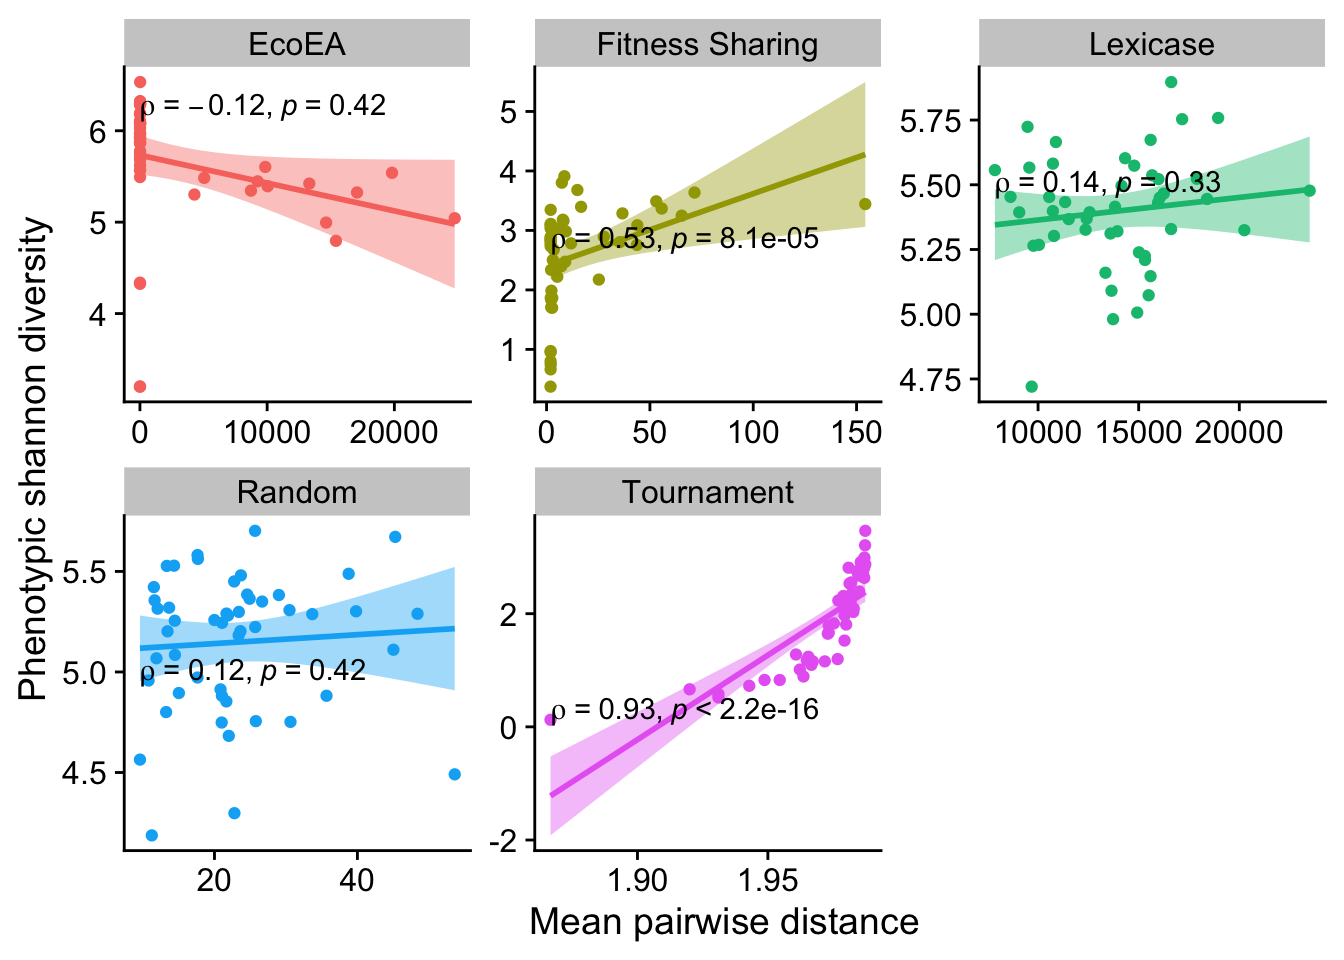
\includegraphics{phylodiversity-in-EC-supplement_files/figure-latex/phen_vs_phylo_shannon_mpd-1.pdf}

\begin{Shaded}
\begin{Highlighting}[]
\KeywordTok{ggplot}\NormalTok{(}
\NormalTok{    data }\OperatorTok\StringTok{ }\KeywordTok{filter}\NormalTok{(gen}\OperatorTok{==}\DecValTok{500000}\NormalTok{),}
    \KeywordTok{aes}\NormalTok{(}
        \DataTypeTok{y=}\NormalTok{phen_diversity,}
        \DataTypeTok{x=}\NormalTok{mean_phenotype_evolutionary_distinctiveness,}
        \DataTypeTok{color=}\NormalTok{selection_name,}
        \DataTypeTok{fill=}\NormalTok{selection_name}
\NormalTok{    )}
\NormalTok{  ) }\OperatorTok{+}
\StringTok{  }\KeywordTok{geom_point}\NormalTok{() }\OperatorTok{+}
\StringTok{    }\KeywordTok{scale_y_continuous}\NormalTok{(}
        \DataTypeTok{name=}\StringTok{"Phenotypic shannon diversity"}
\NormalTok{  ) }\OperatorTok{+}
\StringTok{  }\KeywordTok{scale_x_continuous}\NormalTok{(}
        \DataTypeTok{name=}\StringTok{"Mean evolutionary distinctiveness"}\NormalTok{,}
        \DataTypeTok{breaks =} \KeywordTok{breaks_extended}\NormalTok{(}\DecValTok{4}\NormalTok{)}
\NormalTok{  ) }\OperatorTok{+}\StringTok{ }
\StringTok{  }\KeywordTok{facet_wrap}\NormalTok{(}
      \OperatorTok{~}\NormalTok{selection_name, }\DataTypeTok{scales=}\StringTok{"free"}
\NormalTok{  ) }\OperatorTok{+}\StringTok{ }
\StringTok{  }\KeywordTok{stat_smooth}\NormalTok{(}
    \DataTypeTok{method=}\StringTok{"lm"}
\NormalTok{  ) }\OperatorTok{+}\StringTok{ }
\StringTok{  }\KeywordTok{stat_cor}\NormalTok{(}
    \DataTypeTok{method=}\StringTok{"spearman"}\NormalTok{, }\DataTypeTok{cor.coef.name =} \StringTok{"rho"}\NormalTok{, }\DataTypeTok{color=}\StringTok{"black"}
\NormalTok{  ) }\OperatorTok{+}
\StringTok{  }\KeywordTok{theme}\NormalTok{(}\DataTypeTok{legend.position =} \StringTok{"none"}\NormalTok{)}
\end{Highlighting}
\end{Shaded}

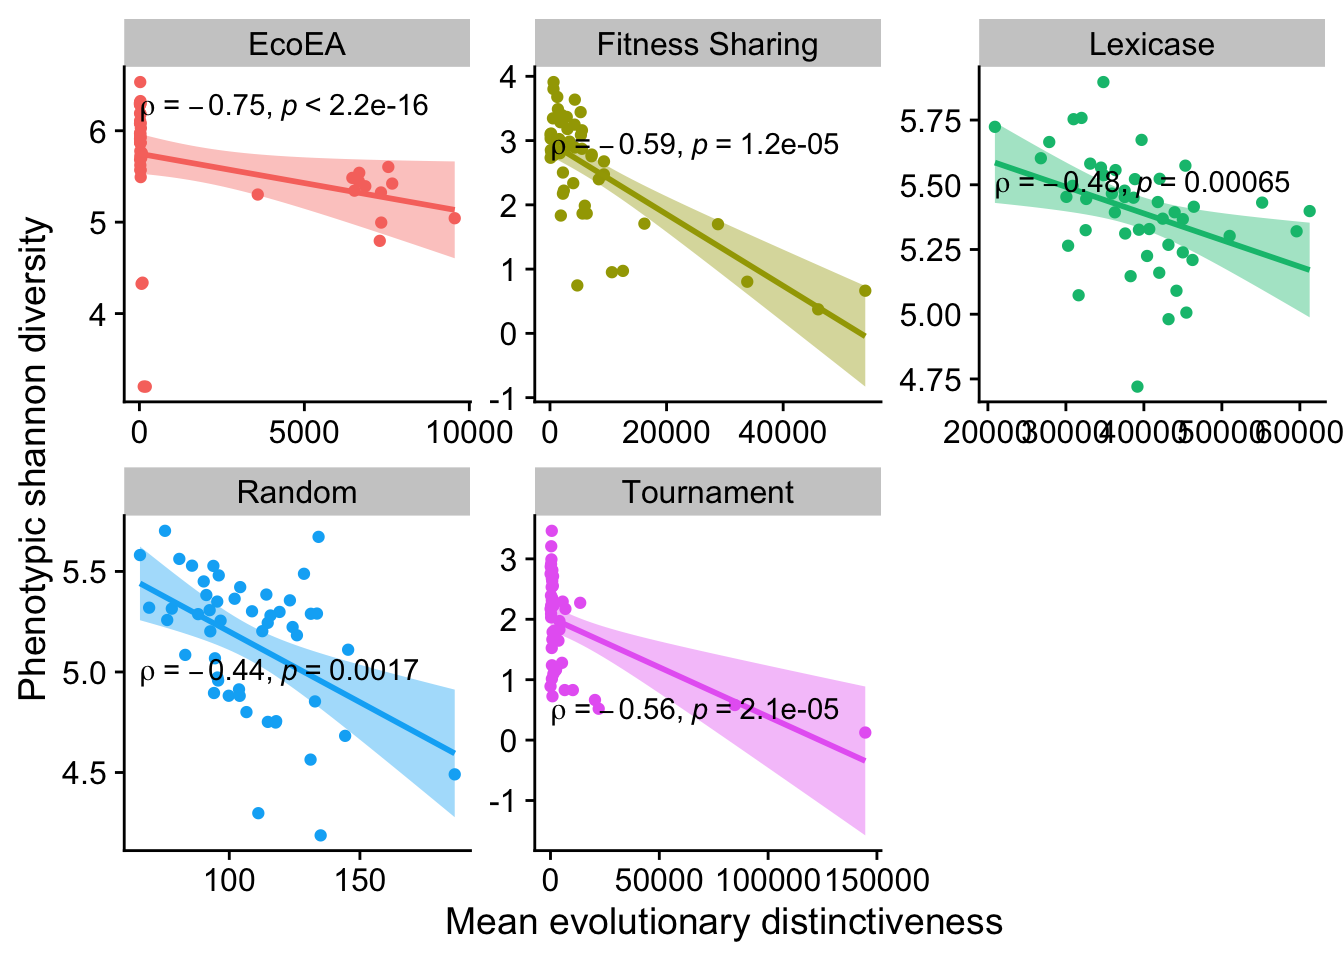
\includegraphics{phylodiversity-in-EC-supplement_files/figure-latex/phen_vs_phylo_shannon_med-1.pdf}

\hypertarget{relationship-between-diversity-and-success}{%
\section{Relationship between diversity and success}\label{relationship-between-diversity-and-success}}

\hypertarget{earlier-in-run}{%
\subsection{Earlier in run}\label{earlier-in-run}}

\begin{Shaded}
\begin{Highlighting}[]
\KeywordTok{ggplot}\NormalTok{(}
\NormalTok{    data }\OperatorTok\StringTok{ }\KeywordTok{filter}\NormalTok{(gen}\OperatorTok{==}\DecValTok{25000}\NormalTok{),}
    \KeywordTok{aes}\NormalTok{(}
        \DataTypeTok{y=}\NormalTok{elite_trait_avg,}
        \DataTypeTok{x=}\NormalTok{mean_phenotype_pairwise_distance,}
        \DataTypeTok{color=}\NormalTok{selection_name,}
        \DataTypeTok{fill=}\NormalTok{selection_name}
\NormalTok{    )}
\NormalTok{  ) }\OperatorTok{+}
\StringTok{  }\KeywordTok{geom_point}\NormalTok{() }\OperatorTok{+}
\StringTok{    }\KeywordTok{scale_y_continuous}\NormalTok{(}
        \DataTypeTok{name=}\StringTok{"Average trait performance"}
\NormalTok{  ) }\OperatorTok{+}
\StringTok{  }\KeywordTok{scale_x_continuous}\NormalTok{(}
        \DataTypeTok{name=}\StringTok{"Mean pairwise distance"}
\NormalTok{  ) }\OperatorTok{+}\StringTok{ }
\StringTok{  }\KeywordTok{facet_wrap}\NormalTok{(}
      \OperatorTok{~}\NormalTok{selection_name, }\DataTypeTok{scales=}\StringTok{"free"}
\NormalTok{  ) }\OperatorTok{+}\StringTok{ }
\StringTok{  }\KeywordTok{stat_smooth}\NormalTok{(}
    \DataTypeTok{method=}\StringTok{"lm"}
\NormalTok{  ) }\OperatorTok{+}\StringTok{ }
\StringTok{  }\KeywordTok{stat_cor}\NormalTok{(}
    \DataTypeTok{method=}\StringTok{"spearman"}\NormalTok{, }\DataTypeTok{cor.coef.name =} \StringTok{"rho"}\NormalTok{, }\DataTypeTok{color=}\StringTok{"black"}
\NormalTok{  ) }\OperatorTok{+}
\StringTok{  }\KeywordTok{theme}\NormalTok{(}\DataTypeTok{legend.position =} \StringTok{"none"}\NormalTok{)}
\end{Highlighting}
\end{Shaded}

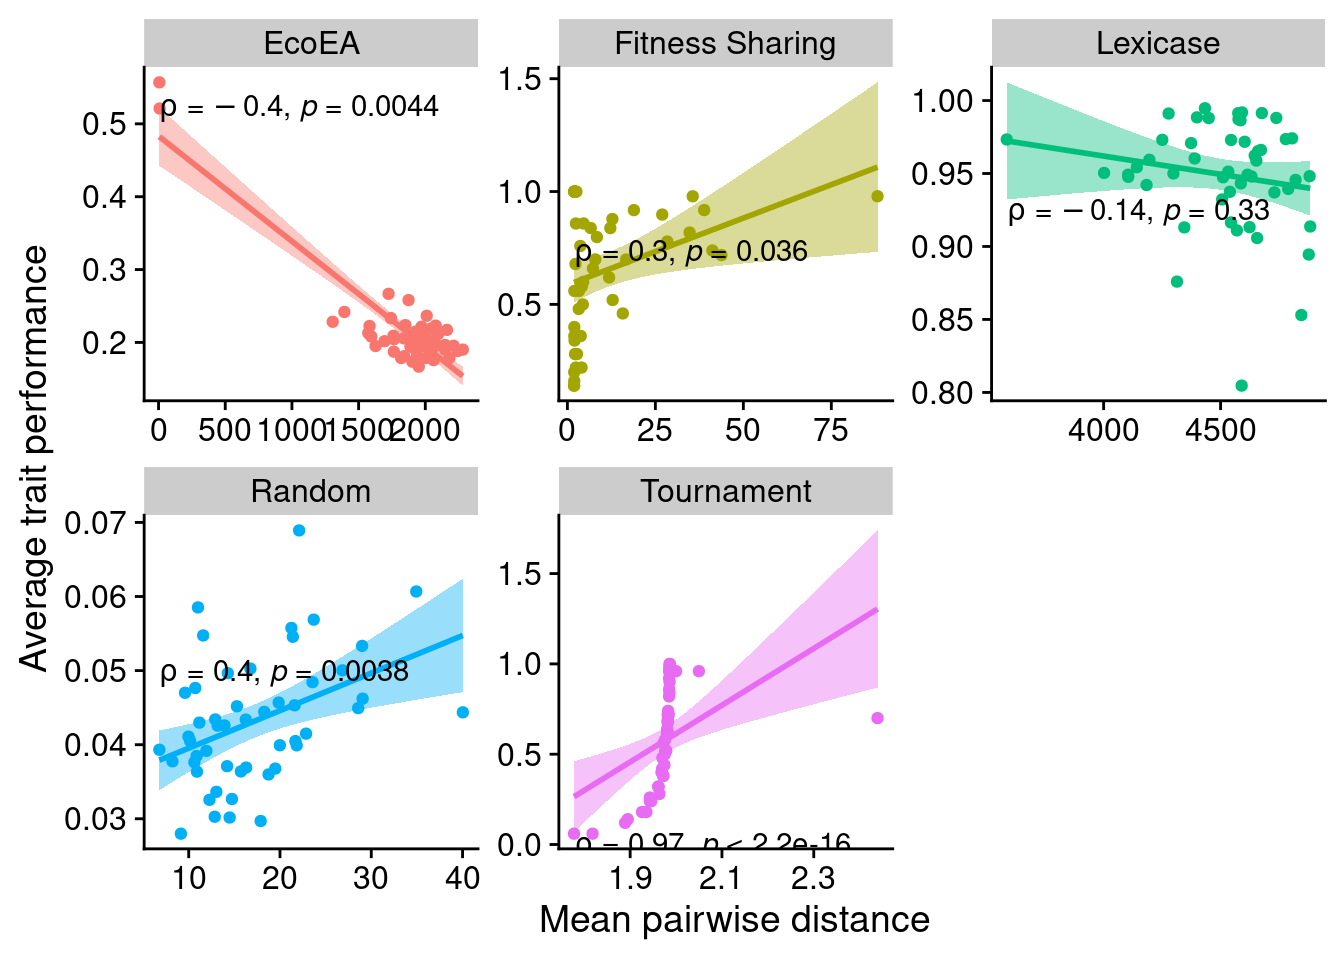
\includegraphics{phylodiversity-in-EC-supplement_files/figure-latex/phylogeny_vs_performance_very_early-1.pdf}

\begin{Shaded}
\begin{Highlighting}[]
\KeywordTok{ggplot}\NormalTok{(}
\NormalTok{    data }\OperatorTok\StringTok{ }\KeywordTok{filter}\NormalTok{(gen}\OperatorTok{==}\DecValTok{25000}\NormalTok{),}
    \KeywordTok{aes}\NormalTok{(}
        \DataTypeTok{y=}\NormalTok{elite_trait_avg,}
        \DataTypeTok{x=}\NormalTok{phen_num_taxa,}
        \DataTypeTok{color=}\NormalTok{selection_name,}
        \DataTypeTok{fill=}\NormalTok{selection_name}
\NormalTok{    )}
\NormalTok{  ) }\OperatorTok{+}
\StringTok{  }\KeywordTok{geom_point}\NormalTok{() }\OperatorTok{+}
\StringTok{    }\KeywordTok{scale_y_continuous}\NormalTok{(}
        \DataTypeTok{name=}\StringTok{"Average trait performance"}
\NormalTok{  ) }\OperatorTok{+}
\StringTok{  }\KeywordTok{scale_x_continuous}\NormalTok{(}
        \DataTypeTok{name=}\StringTok{"Phenotypic richness"}
\NormalTok{  ) }\OperatorTok{+}\StringTok{ }
\StringTok{  }\KeywordTok{facet_wrap}\NormalTok{(}
      \OperatorTok{~}\NormalTok{selection_name, }\DataTypeTok{scales=}\StringTok{"free"}
\NormalTok{  ) }\OperatorTok{+}\StringTok{ }
\StringTok{  }\KeywordTok{stat_smooth}\NormalTok{(}
    \DataTypeTok{method=}\StringTok{"lm"}
\NormalTok{  ) }\OperatorTok{+}\StringTok{ }
\StringTok{  }\KeywordTok{stat_cor}\NormalTok{(}
    \DataTypeTok{method=}\StringTok{"spearman"}\NormalTok{, }\DataTypeTok{cor.coef.name =} \StringTok{"rho"}\NormalTok{, }\DataTypeTok{color=}\StringTok{"black"}
\NormalTok{  ) }\OperatorTok{+}
\StringTok{  }\KeywordTok{theme}\NormalTok{(}\DataTypeTok{legend.position =} \StringTok{"none"}\NormalTok{)}
\end{Highlighting}
\end{Shaded}

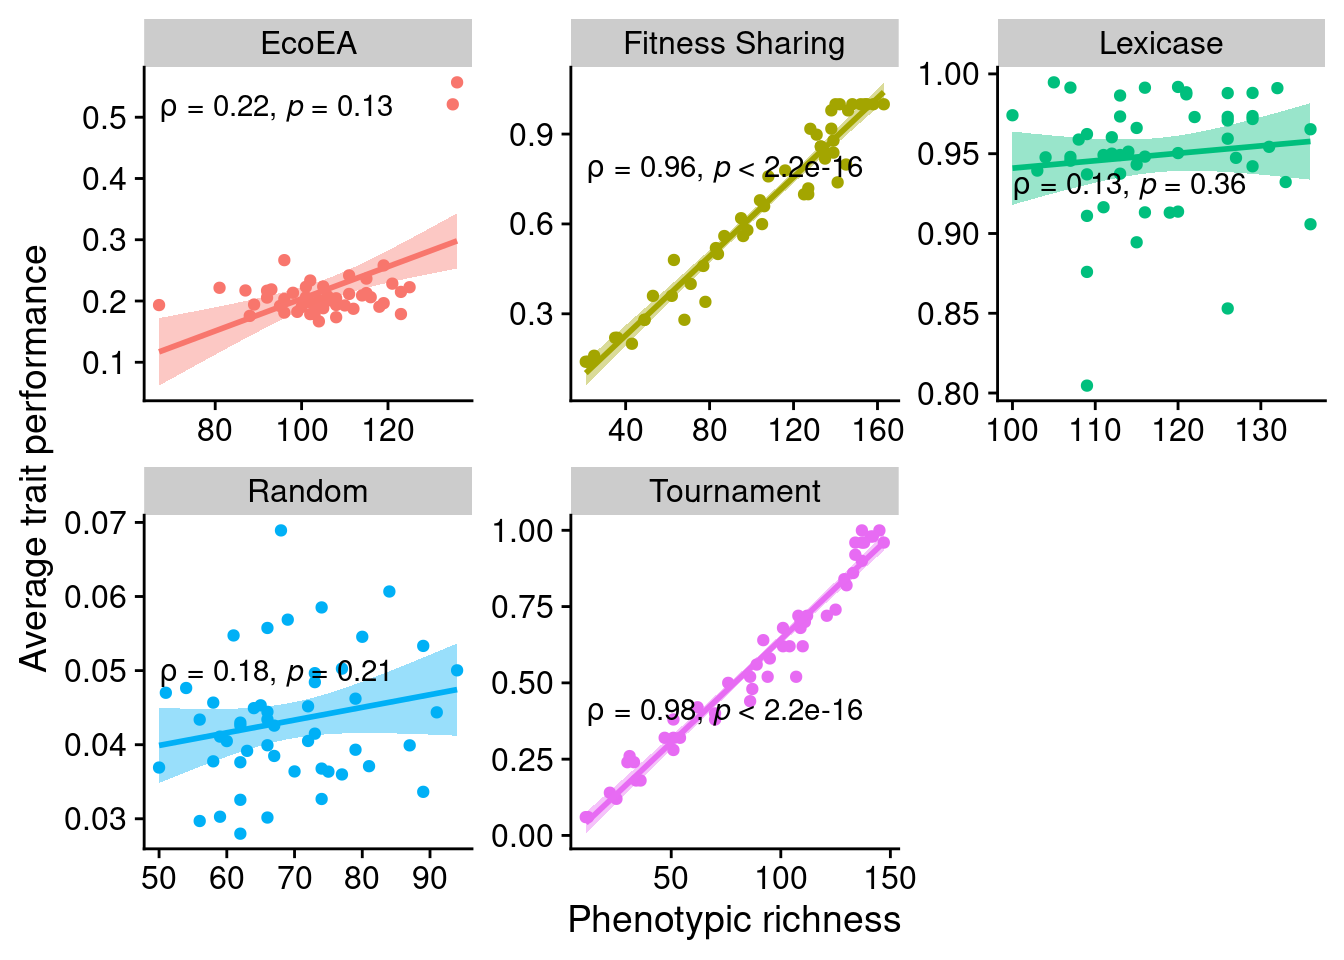
\includegraphics{phylodiversity-in-EC-supplement_files/figure-latex/richness_vs_performance_very_early-1.pdf}

\begin{Shaded}
\begin{Highlighting}[]
\NormalTok{phylogney_vs_performance <-}\StringTok{ }\KeywordTok{ggplot}\NormalTok{(}
\NormalTok{    data }\OperatorTok\StringTok{ }\KeywordTok{filter}\NormalTok{(gen}\OperatorTok{==}\DecValTok{50000}\NormalTok{),}
    \KeywordTok{aes}\NormalTok{(}
        \DataTypeTok{y=}\NormalTok{elite_trait_avg,}
        \DataTypeTok{x=}\NormalTok{mean_phenotype_pairwise_distance,}
        \DataTypeTok{color=}\NormalTok{selection_name,}
        \DataTypeTok{fill=}\NormalTok{selection_name}
\NormalTok{    )}
\NormalTok{  ) }\OperatorTok{+}
\StringTok{  }\KeywordTok{geom_point}\NormalTok{() }\OperatorTok{+}
\StringTok{    }\KeywordTok{scale_y_continuous}\NormalTok{(}
        \DataTypeTok{name=}\StringTok{"Average trait performance"}
\NormalTok{  ) }\OperatorTok{+}
\StringTok{  }\KeywordTok{scale_x_continuous}\NormalTok{(}
        \DataTypeTok{name=}\StringTok{"Mean pairwise distance"}
\NormalTok{  ) }\OperatorTok{+}\StringTok{ }
\StringTok{  }\KeywordTok{facet_wrap}\NormalTok{(}
      \OperatorTok{~}\NormalTok{selection_name, }\DataTypeTok{scales=}\StringTok{"free"}
\NormalTok{  ) }\OperatorTok{+}\StringTok{ }
\StringTok{  }\KeywordTok{stat_smooth}\NormalTok{(}
    \DataTypeTok{method=}\StringTok{"lm"}
\NormalTok{  ) }\OperatorTok{+}\StringTok{ }
\StringTok{  }\KeywordTok{stat_cor}\NormalTok{(}
    \DataTypeTok{method=}\StringTok{"spearman"}\NormalTok{, }\DataTypeTok{cor.coef.name =} \StringTok{"rho"}\NormalTok{, }\DataTypeTok{color=}\StringTok{"black"}
\NormalTok{  ) }\OperatorTok{+}
\StringTok{  }\KeywordTok{theme}\NormalTok{(}\DataTypeTok{legend.position =} \StringTok{"none"}\NormalTok{)}
  
\NormalTok{phylogney_vs_performance}
\end{Highlighting}
\end{Shaded}

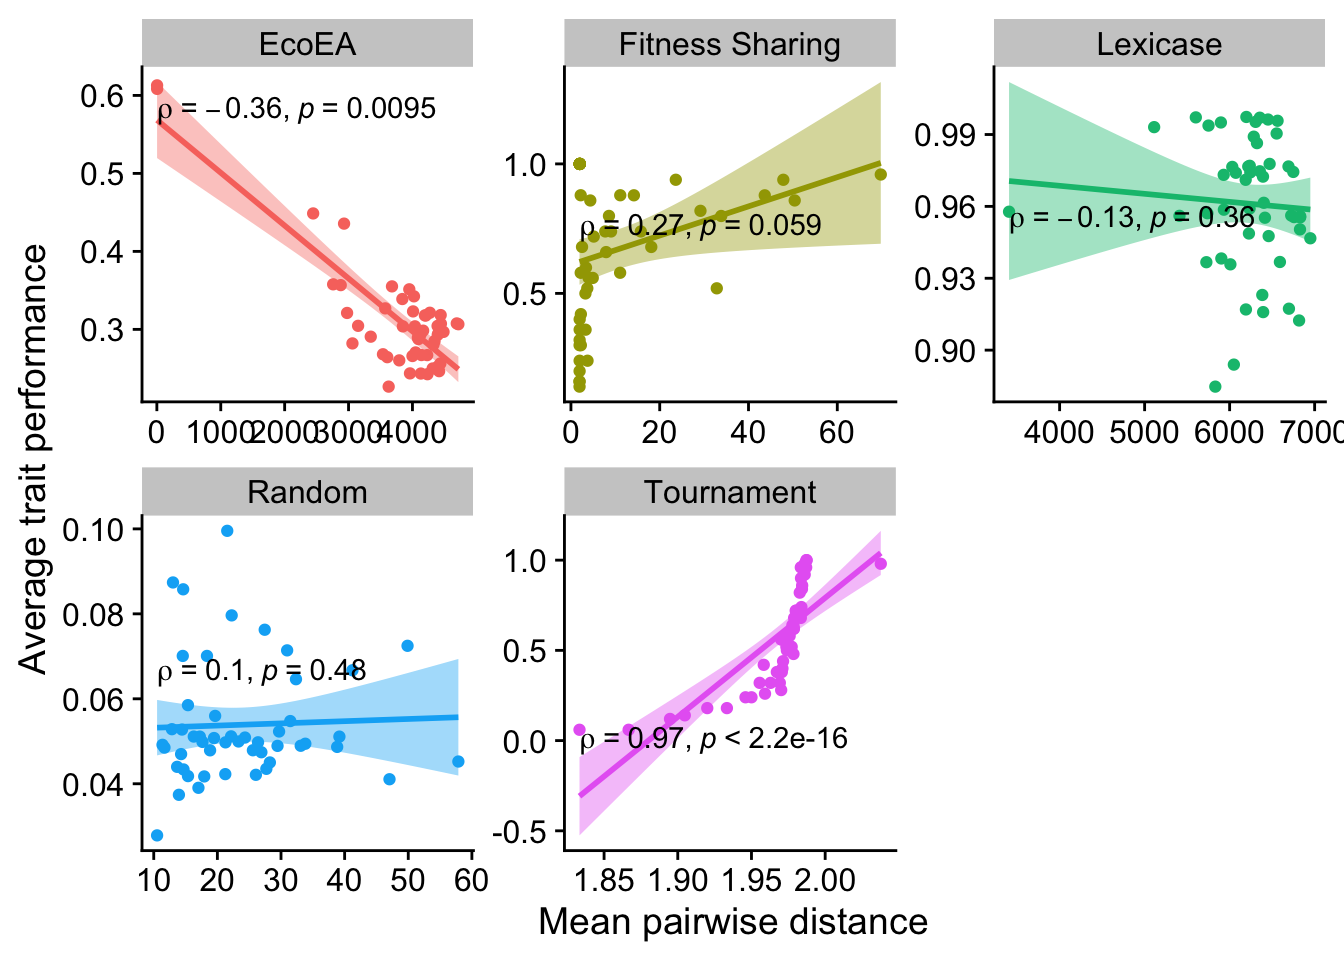
\includegraphics{phylodiversity-in-EC-supplement_files/figure-latex/phylogeny_vs_performance_early-1.pdf}

\begin{Shaded}
\begin{Highlighting}[]
\NormalTok{richness_vs_performance <-}\StringTok{ }\KeywordTok{ggplot}\NormalTok{(}
\NormalTok{    data }\OperatorTok\StringTok{ }\KeywordTok{filter}\NormalTok{(gen}\OperatorTok{==}\DecValTok{50000}\NormalTok{),}
    \KeywordTok{aes}\NormalTok{(}
        \DataTypeTok{y=}\NormalTok{elite_trait_avg,}
        \DataTypeTok{x=}\NormalTok{phen_num_taxa,}
        \DataTypeTok{color=}\NormalTok{selection_name,}
        \DataTypeTok{fill=}\NormalTok{selection_name}
\NormalTok{    )}
\NormalTok{  ) }\OperatorTok{+}
\StringTok{  }\KeywordTok{geom_point}\NormalTok{() }\OperatorTok{+}
\StringTok{    }\KeywordTok{scale_y_continuous}\NormalTok{(}
        \DataTypeTok{name=}\StringTok{"Average trait performance"}
\NormalTok{  ) }\OperatorTok{+}
\StringTok{  }\KeywordTok{scale_x_continuous}\NormalTok{(}
        \DataTypeTok{name=}\StringTok{"Phenotypic richness"}
\NormalTok{  ) }\OperatorTok{+}\StringTok{ }
\StringTok{  }\KeywordTok{facet_wrap}\NormalTok{(}
      \OperatorTok{~}\NormalTok{selection_name, }\DataTypeTok{scales=}\StringTok{"free"}
\NormalTok{  ) }\OperatorTok{+}\StringTok{ }
\StringTok{  }\KeywordTok{stat_smooth}\NormalTok{(}
    \DataTypeTok{method=}\StringTok{"lm"}
\NormalTok{  ) }\OperatorTok{+}\StringTok{ }
\StringTok{  }\KeywordTok{stat_cor}\NormalTok{(}
    \DataTypeTok{method=}\StringTok{"spearman"}\NormalTok{, }\DataTypeTok{cor.coef.name =} \StringTok{"rho"}\NormalTok{, }\DataTypeTok{color=}\StringTok{"black"}
\NormalTok{  ) }\OperatorTok{+}
\StringTok{  }\KeywordTok{theme}\NormalTok{(}\DataTypeTok{legend.position =} \StringTok{"none"}\NormalTok{)}
  
\NormalTok{richness_vs_performance}
\end{Highlighting}
\end{Shaded}

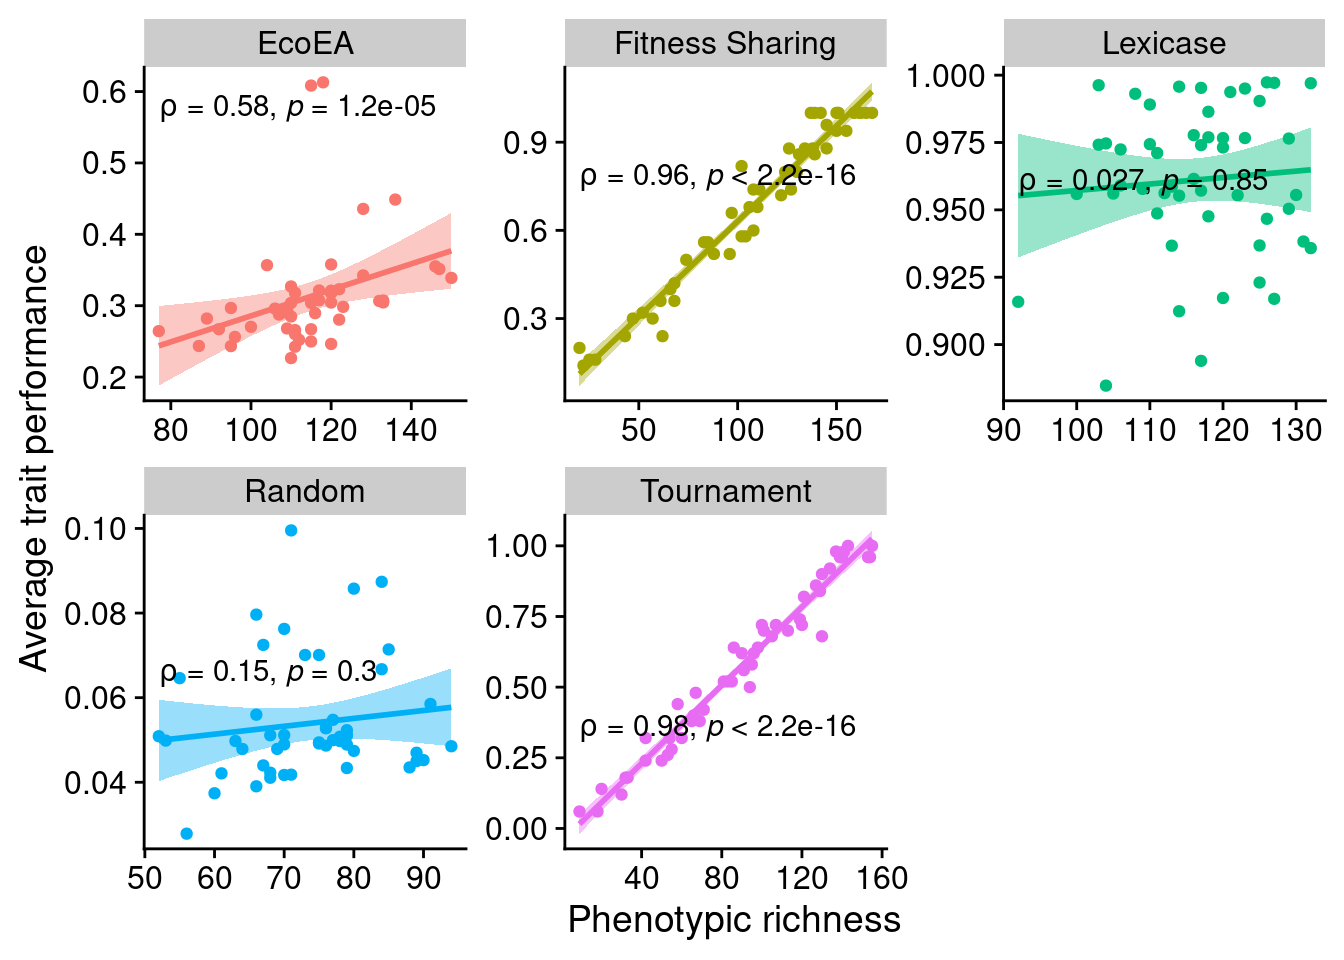
\includegraphics{phylodiversity-in-EC-supplement_files/figure-latex/richness_vs_performance_early-1.pdf}

\hypertarget{end-of-run}{%
\subsection{End of run}\label{end-of-run}}

\begin{Shaded}
\begin{Highlighting}[]
\NormalTok{final_phylogney_vs_performance <-}\StringTok{ }\KeywordTok{ggplot}\NormalTok{(}
\NormalTok{    final_data,}
    \KeywordTok{aes}\NormalTok{(}
        \DataTypeTok{y=}\NormalTok{elite_trait_avg,}
        \DataTypeTok{x=}\NormalTok{mean_phenotype_pairwise_distance,}
        \DataTypeTok{color=}\NormalTok{selection_name,}
        \DataTypeTok{fill=}\NormalTok{selection_name}
\NormalTok{    )}
\NormalTok{  ) }\OperatorTok{+}
\StringTok{  }\KeywordTok{geom_point}\NormalTok{() }\OperatorTok{+}
\StringTok{    }\KeywordTok{scale_y_continuous}\NormalTok{(}
        \DataTypeTok{name=}\StringTok{"Average trait performance"}
\NormalTok{  ) }\OperatorTok{+}
\StringTok{  }\KeywordTok{scale_x_continuous}\NormalTok{(}
        \DataTypeTok{name=}\StringTok{"Mean pairwise distance"}
\NormalTok{  ) }\OperatorTok{+}\StringTok{ }
\StringTok{  }\KeywordTok{facet_wrap}\NormalTok{(}
      \OperatorTok{~}\NormalTok{selection_name, }\DataTypeTok{scales=}\StringTok{"free"}
\NormalTok{  ) }\OperatorTok{+}\StringTok{ }
\StringTok{  }\KeywordTok{stat_smooth}\NormalTok{(}
    \DataTypeTok{method=}\StringTok{"lm"}
\NormalTok{  ) }\OperatorTok{+}\StringTok{ }
\StringTok{  }\KeywordTok{stat_cor}\NormalTok{(}
    \DataTypeTok{method=}\StringTok{"spearman"}\NormalTok{, }\DataTypeTok{cor.coef.name =} \StringTok{"rho"}\NormalTok{, }\DataTypeTok{color=}\StringTok{"black"}
\NormalTok{  ) }\OperatorTok{+}
\StringTok{  }\KeywordTok{theme}\NormalTok{(}\DataTypeTok{legend.position =} \StringTok{"none"}\NormalTok{)}
  
\NormalTok{final_phylogney_vs_performance}
\end{Highlighting}
\end{Shaded}

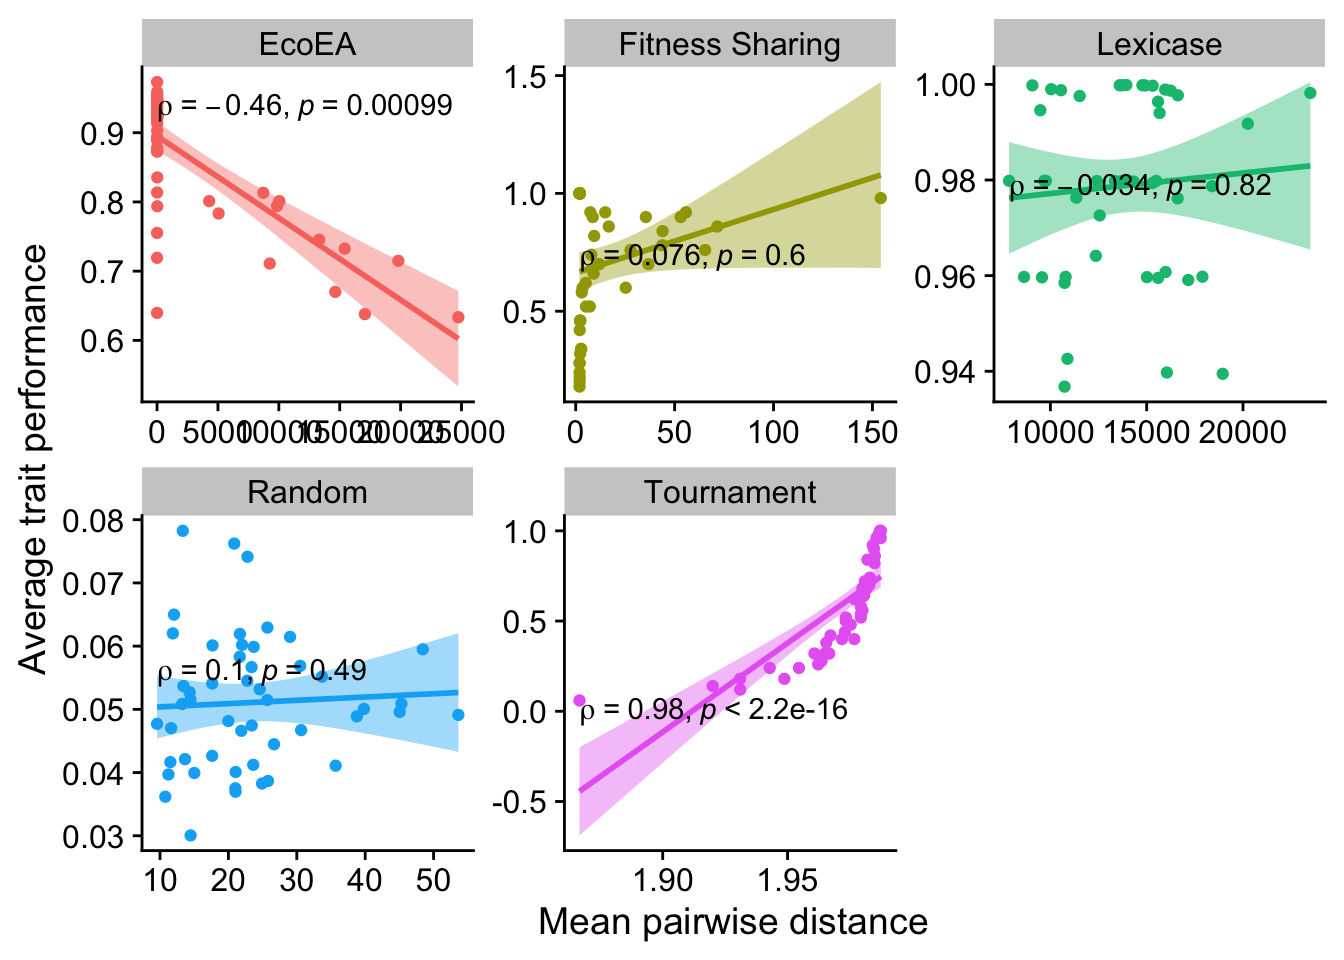
\includegraphics{phylodiversity-in-EC-supplement_files/figure-latex/phylogeny_vs_performance-1.pdf}

\begin{Shaded}
\begin{Highlighting}[]
\NormalTok{final_richness_vs_performance <-}\StringTok{ }\KeywordTok{ggplot}\NormalTok{(}
\NormalTok{    final_data,}
    \KeywordTok{aes}\NormalTok{(}
        \DataTypeTok{y=}\NormalTok{elite_trait_avg,}
        \DataTypeTok{x=}\NormalTok{phen_num_taxa,}
        \DataTypeTok{color=}\NormalTok{selection_name,}
        \DataTypeTok{fill=}\NormalTok{selection_name}
\NormalTok{    )}
\NormalTok{  ) }\OperatorTok{+}
\StringTok{  }\KeywordTok{geom_point}\NormalTok{() }\OperatorTok{+}
\StringTok{    }\KeywordTok{scale_y_continuous}\NormalTok{(}
        \DataTypeTok{name=}\StringTok{"Average trait performance"}
\NormalTok{  ) }\OperatorTok{+}
\StringTok{  }\KeywordTok{scale_x_continuous}\NormalTok{(}
        \DataTypeTok{name=}\StringTok{"Phenotypic richness"}
\NormalTok{  ) }\OperatorTok{+}\StringTok{ }
\StringTok{  }\KeywordTok{facet_wrap}\NormalTok{(}
      \OperatorTok{~}\NormalTok{selection_name, }\DataTypeTok{scales=}\StringTok{"free"}
\NormalTok{  ) }\OperatorTok{+}\StringTok{ }
\StringTok{  }\KeywordTok{stat_smooth}\NormalTok{(}
    \DataTypeTok{method=}\StringTok{"lm"}
\NormalTok{  ) }\OperatorTok{+}\StringTok{ }
\StringTok{  }\KeywordTok{stat_cor}\NormalTok{(}
    \DataTypeTok{method=}\StringTok{"spearman"}\NormalTok{, }\DataTypeTok{cor.coef.name =} \StringTok{"rho"}\NormalTok{, }\DataTypeTok{color=}\StringTok{"black"}
\NormalTok{  ) }\OperatorTok{+}
\StringTok{  }\KeywordTok{theme}\NormalTok{(}\DataTypeTok{legend.position =} \StringTok{"none"}\NormalTok{)}
  
\NormalTok{final_richness_vs_performance}
\end{Highlighting}
\end{Shaded}

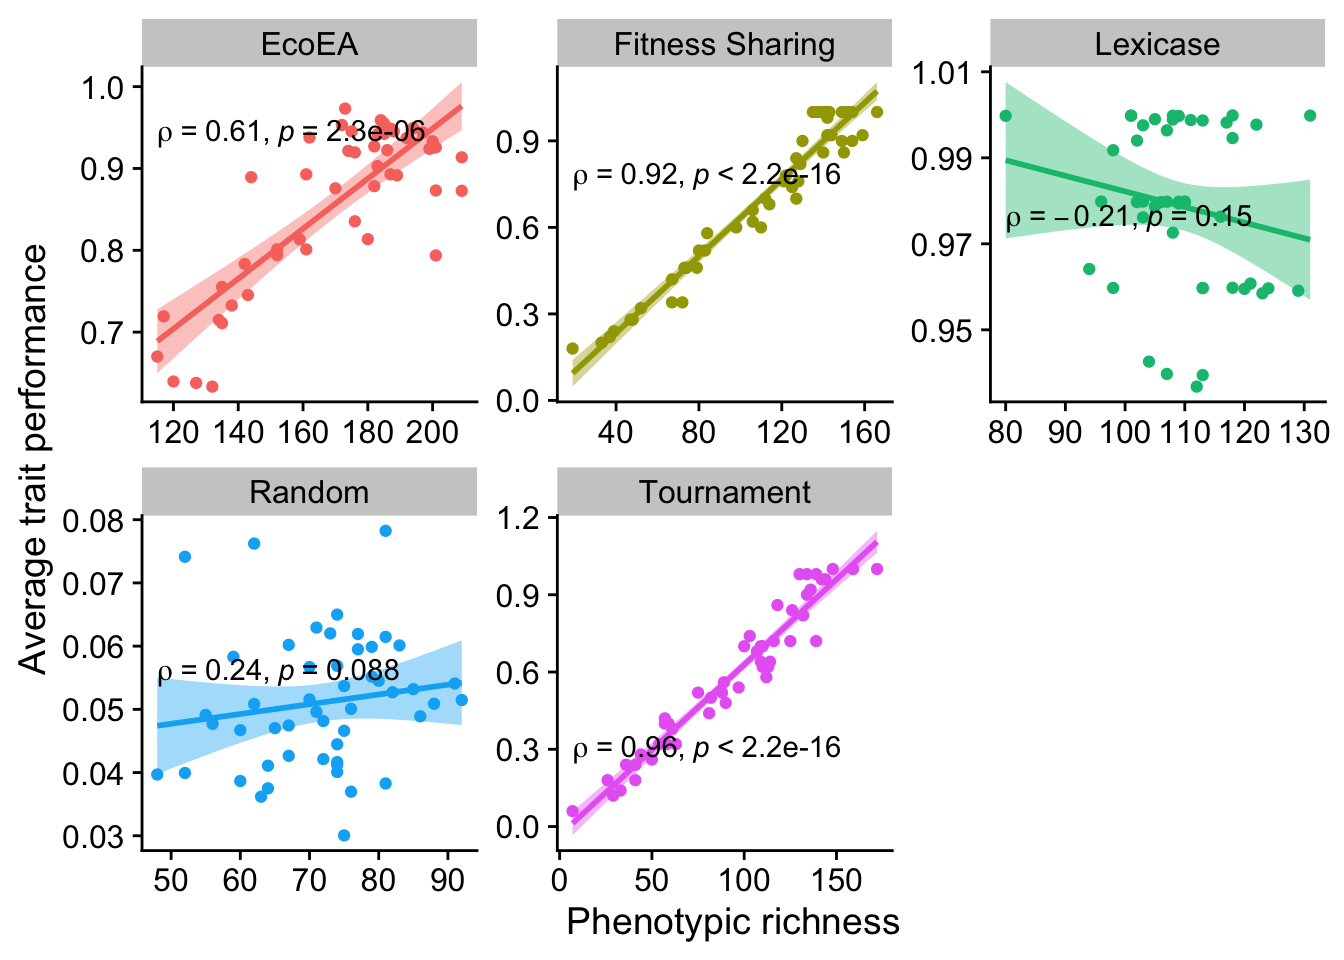
\includegraphics{phylodiversity-in-EC-supplement_files/figure-latex/richness_vs_performance-1.pdf}

\hypertarget{causality-analysis}{%
\section{Causality analysis}\label{causality-analysis}}

\hypertarget{transfer-entropy-from-diversity-to-fitness}{%
\subsection{Transfer entropy from diversity to fitness}\label{transfer-entropy-from-diversity-to-fitness}}

\hypertarget{max-pairwise-distance-vs.phenotypic-richness}{%
\subsubsection{Max pairwise distance vs.~phenotypic richness}\label{max-pairwise-distance-vs.phenotypic-richness}}

\begin{Shaded}
\begin{Highlighting}[]
\CommentTok{# Calculate transfer entropy for max pairwise distance}
\CommentTok{# Time points are 10 generations, so calculating lag 1 gives us lag 10}
\NormalTok{res <-}\StringTok{ }\NormalTok{data }\OperatorTok\StringTok{ }\KeywordTok{group_by}\NormalTok{(directory, selection_name) }\OperatorTok
\KeywordTok{summarise}\NormalTok{(}
  \DataTypeTok{fit_phylo_10 =}     \KeywordTok{condinformation}\NormalTok{(}\KeywordTok{discretize}\NormalTok{(elite_trait_avg), }\CommentTok{# TE phylo -> fit, lag 10}
                                     \KeywordTok{discretize}\NormalTok{(}\KeywordTok{lag}\NormalTok{(max_phenotype_pairwise_distance, }\DecValTok{1}\NormalTok{)), }
                                     \KeywordTok{discretize}\NormalTok{(}\KeywordTok{lag}\NormalTok{(elite_trait_avg, }\DecValTok{1}\NormalTok{))),}
  \DataTypeTok{fit_phylo_100 =}    \KeywordTok{condinformation}\NormalTok{(}\KeywordTok{discretize}\NormalTok{(elite_trait_avg), }\CommentTok{# TE phylo -> fit, lag 100}
                                     \KeywordTok{discretize}\NormalTok{(}\KeywordTok{lag}\NormalTok{(max_phenotype_pairwise_distance, }\DecValTok{10}\NormalTok{)), }
                                     \KeywordTok{discretize}\NormalTok{(}\KeywordTok{lag}\NormalTok{(elite_trait_avg, }\DecValTok{10}\NormalTok{))),}
  \DataTypeTok{fit_phylo_1000 =}   \KeywordTok{condinformation}\NormalTok{(}\KeywordTok{discretize}\NormalTok{(elite_trait_avg), }\CommentTok{# TE phylo -> fit, lag 1000}
                                     \KeywordTok{discretize}\NormalTok{(}\KeywordTok{lag}\NormalTok{(max_phenotype_pairwise_distance, }\DecValTok{100}\NormalTok{)), }
                                     \KeywordTok{discretize}\NormalTok{(}\KeywordTok{lag}\NormalTok{(elite_trait_avg, }\DecValTok{100}\NormalTok{))),}
  \DataTypeTok{fit_phylo_10000 =}  \KeywordTok{condinformation}\NormalTok{(}\KeywordTok{discretize}\NormalTok{(elite_trait_avg), }\CommentTok{# TE phylo -> fit, lag 10000}
                                     \KeywordTok{discretize}\NormalTok{(}\KeywordTok{lag}\NormalTok{(max_phenotype_pairwise_distance, }\DecValTok{1000}\NormalTok{)), }
                                     \KeywordTok{discretize}\NormalTok{(}\KeywordTok{lag}\NormalTok{(elite_trait_avg, }\DecValTok{1000}\NormalTok{))),}
  \DataTypeTok{fit_phylo_100000 =} \KeywordTok{condinformation}\NormalTok{(}\KeywordTok{discretize}\NormalTok{(elite_trait_avg), }\CommentTok{# TE phylo -> fit, lag 100000}
                                     \KeywordTok{discretize}\NormalTok{(}\KeywordTok{lag}\NormalTok{(max_phenotype_pairwise_distance, }\DecValTok{10000}\NormalTok{)), }
                                     \KeywordTok{discretize}\NormalTok{(}\KeywordTok{lag}\NormalTok{(elite_trait_avg, }\DecValTok{10000}\NormalTok{))),  }
  \DataTypeTok{fit_fit_10000 =}    \KeywordTok{condinformation}\NormalTok{(}\KeywordTok{discretize}\NormalTok{(elite_trait_avg), }\CommentTok{# Mutual info btwn. fit and lagged fit}
                                     \KeywordTok{discretize}\NormalTok{(}\KeywordTok{lag}\NormalTok{(elite_trait_avg, }\DecValTok{1000}\NormalTok{)), }
                                     \KeywordTok{discretize}\NormalTok{(}\KeywordTok{lag}\NormalTok{(max_phenotype_pairwise_distance, }\DecValTok{1000}\NormalTok{))),}
  \DataTypeTok{fit_fit_100000 =}   \KeywordTok{condinformation}\NormalTok{(}\KeywordTok{discretize}\NormalTok{(elite_trait_avg), }\CommentTok{# Mutual info btwn. fit and lagged fit}
                                     \KeywordTok{discretize}\NormalTok{(}\KeywordTok{lag}\NormalTok{(elite_trait_avg, }\DecValTok{10000}\NormalTok{)), }
                                     \KeywordTok{discretize}\NormalTok{(}\KeywordTok{lag}\NormalTok{(max_phenotype_pairwise_distance, }\DecValTok{10000}\NormalTok{))),  }
  \DataTypeTok{fit_pheno_10 =}     \KeywordTok{condinformation}\NormalTok{(}\KeywordTok{discretize}\NormalTok{(elite_trait_avg), }\CommentTok{# TE pheno -> fit, lag 10}
                                     \KeywordTok{discretize}\NormalTok{(}\KeywordTok{lag}\NormalTok{(phen_num_taxa, }\DecValTok{1}\NormalTok{)), }
                                     \KeywordTok{discretize}\NormalTok{(}\KeywordTok{lag}\NormalTok{(elite_trait_avg, }\DecValTok{1}\NormalTok{))),}
  \DataTypeTok{fit_pheno_100 =}    \KeywordTok{condinformation}\NormalTok{(}\KeywordTok{discretize}\NormalTok{(elite_trait_avg),  }\CommentTok{# TE pheno -> fit, lag 100 }
                                     \KeywordTok{discretize}\NormalTok{(}\KeywordTok{lag}\NormalTok{(phen_num_taxa, }\DecValTok{10}\NormalTok{)), }
                                     \KeywordTok{discretize}\NormalTok{(}\KeywordTok{lag}\NormalTok{(elite_trait_avg, }\DecValTok{10}\NormalTok{))),}
  \DataTypeTok{fit_pheno_1000 =}   \KeywordTok{condinformation}\NormalTok{(}\KeywordTok{discretize}\NormalTok{(elite_trait_avg),  }\CommentTok{# TE pheno -> fit, lag 1000}
                                     \KeywordTok{discretize}\NormalTok{(}\KeywordTok{lag}\NormalTok{(phen_num_taxa, }\DecValTok{100}\NormalTok{)), }
                                     \KeywordTok{discretize}\NormalTok{(}\KeywordTok{lag}\NormalTok{(elite_trait_avg, }\DecValTok{100}\NormalTok{))),}
  \DataTypeTok{fit_pheno_10000 =}  \KeywordTok{condinformation}\NormalTok{(}\KeywordTok{discretize}\NormalTok{(elite_trait_avg),  }\CommentTok{# TE pheno -> fit, lag 10000}
                                     \KeywordTok{discretize}\NormalTok{(}\KeywordTok{lag}\NormalTok{(phen_num_taxa, }\DecValTok{1000}\NormalTok{)), }
                                     \KeywordTok{discretize}\NormalTok{(}\KeywordTok{lag}\NormalTok{(elite_trait_avg, }\DecValTok{1000}\NormalTok{))),}
  \DataTypeTok{fit_pheno_100000 =} \KeywordTok{condinformation}\NormalTok{(}\KeywordTok{discretize}\NormalTok{(elite_trait_avg),  }\CommentTok{# TE pheno -> fit, lag 100000}
                                     \KeywordTok{discretize}\NormalTok{(}\KeywordTok{lag}\NormalTok{(phen_num_taxa, }\DecValTok{10000}\NormalTok{)), }
                                     \KeywordTok{discretize}\NormalTok{(}\KeywordTok{lag}\NormalTok{(elite_trait_avg, }\DecValTok{10000}\NormalTok{)))}
\NormalTok{)}

\CommentTok{# Turn Transfer Entropy columns into rows}
\NormalTok{res <-}\StringTok{ }\NormalTok{res }\OperatorTok\StringTok{ }\KeywordTok{pivot_longer}\NormalTok{(}\DataTypeTok{cols=}\KeywordTok{contains}\NormalTok{(}\StringTok{"o_10"}\NormalTok{))}
\CommentTok{# Pull lag into a column}
\NormalTok{res}\OperatorTok{$}\NormalTok{offset <-}\StringTok{ }\KeywordTok{str_extract}\NormalTok{(res}\OperatorTok{$}\NormalTok{name, }\StringTok{"[:digit:]*$"}\NormalTok{)}
\CommentTok{# Make column indicating direction of transfer entropy}
\NormalTok{res}\OperatorTok{$}\NormalTok{Type <-}\StringTok{ }\KeywordTok{case_when}\NormalTok{(}\KeywordTok{str_detect}\NormalTok{(res}\OperatorTok{$}\NormalTok{name, }\StringTok{"phylo"}\NormalTok{) }\OperatorTok{~}\StringTok{ "Phylogenetic"}\NormalTok{, }\OtherTok{TRUE} \OperatorTok{~}\StringTok{ "Phenotypic"}\NormalTok{)}

\CommentTok{# Plot transfer entropy}
\KeywordTok{ggplot}\NormalTok{(}
\NormalTok{  res }\OperatorTok\StringTok{ }\KeywordTok{filter}\NormalTok{(}\KeywordTok{str_detect}\NormalTok{(name, }\StringTok{"fit_ph*"}\NormalTok{)), }
  \KeywordTok{aes}\NormalTok{(}
    \DataTypeTok{x=}\KeywordTok{as.factor}\NormalTok{(offset), }
    \DataTypeTok{y=}\NormalTok{value, }
    \DataTypeTok{color=}\NormalTok{Type}
\NormalTok{    )}
\NormalTok{  ) }\OperatorTok{+}\StringTok{ }
\StringTok{  }\KeywordTok{geom_boxplot}\NormalTok{() }\OperatorTok{+}\StringTok{ }
\StringTok{  }\KeywordTok{facet_wrap}\NormalTok{(}\OperatorTok{~}\NormalTok{selection_name) }\OperatorTok{+}\StringTok{ }
\StringTok{  }\KeywordTok{scale_x_discrete}\NormalTok{(}\StringTok{"Lag"}\NormalTok{,}\DataTypeTok{labels=}\KeywordTok{c}\NormalTok{(}\StringTok{"10"}\NormalTok{,}\StringTok{""}\NormalTok{,}\StringTok{"1000"}\NormalTok{,}\StringTok{""}\NormalTok{,}\StringTok{"100000"}\NormalTok{)) }\OperatorTok{+}\StringTok{ }
\StringTok{  }\KeywordTok{scale_y_continuous}\NormalTok{(}\StringTok{"Transfer Entropy"}\NormalTok{) }\OperatorTok{+}\StringTok{ }
\StringTok{  }\KeywordTok{theme}\NormalTok{(}\DataTypeTok{legend.position =} \KeywordTok{c}\NormalTok{(}\DecValTok{1}\NormalTok{, }\DecValTok{0}\NormalTok{),}
        \DataTypeTok{legend.justification =} \KeywordTok{c}\NormalTok{(}\DecValTok{1}\NormalTok{, }\DecValTok{0}\NormalTok{)) }\OperatorTok{+}\StringTok{ }
\StringTok{  }\KeywordTok{scale_color_discrete}\NormalTok{(}\StringTok{""}\NormalTok{)}
\end{Highlighting}
\end{Shaded}

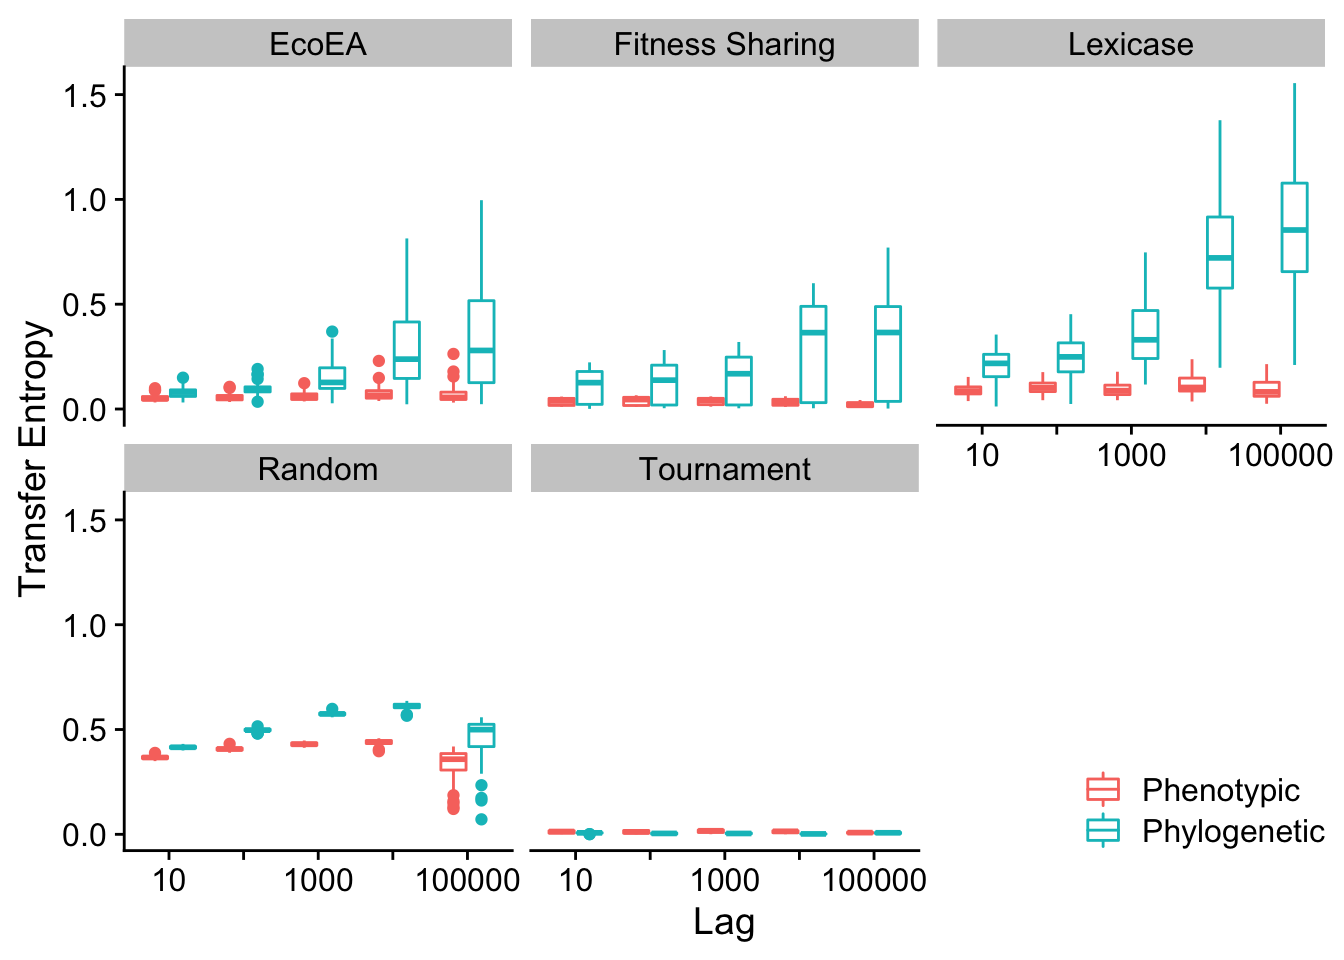
\includegraphics{phylodiversity-in-EC-supplement_files/figure-latex/information_theory-1.pdf}

\hypertarget{mean-pairwise-distance-vs.phenotypic-richness}{%
\subsubsection{Mean pairwise distance vs.~phenotypic richness}\label{mean-pairwise-distance-vs.phenotypic-richness}}

\begin{Shaded}
\begin{Highlighting}[]
\CommentTok{# Calculate transfer entropy for mean pairwise distance}
\CommentTok{# Time points are 10 generations, so calculating lag 1 gives us lag 10}
\NormalTok{res <-}\StringTok{ }\NormalTok{data }\OperatorTok\StringTok{ }\KeywordTok{group_by}\NormalTok{(directory, selection_name) }\OperatorTok
\KeywordTok{summarise}\NormalTok{(}
  \DataTypeTok{fit_phylo_10 =}     \KeywordTok{condinformation}\NormalTok{(}\KeywordTok{discretize}\NormalTok{(elite_trait_avg), }\CommentTok{# TE phylo -> fit, lag 10}
                                     \KeywordTok{discretize}\NormalTok{(}\KeywordTok{lag}\NormalTok{(mean_phenotype_pairwise_distance, }\DecValTok{1}\NormalTok{)), }
                                     \KeywordTok{discretize}\NormalTok{(}\KeywordTok{lag}\NormalTok{(elite_trait_avg, }\DecValTok{1}\NormalTok{))),}
  \DataTypeTok{fit_phylo_100 =}    \KeywordTok{condinformation}\NormalTok{(}\KeywordTok{discretize}\NormalTok{(elite_trait_avg), }\CommentTok{# TE phylo -> fit, lag 100}
                                     \KeywordTok{discretize}\NormalTok{(}\KeywordTok{lag}\NormalTok{(mean_phenotype_pairwise_distance, }\DecValTok{10}\NormalTok{)), }
                                     \KeywordTok{discretize}\NormalTok{(}\KeywordTok{lag}\NormalTok{(elite_trait_avg, }\DecValTok{10}\NormalTok{))),}
  \DataTypeTok{fit_phylo_1000 =}   \KeywordTok{condinformation}\NormalTok{(}\KeywordTok{discretize}\NormalTok{(elite_trait_avg), }\CommentTok{# TE phylo -> fit, lag 1000}
                                     \KeywordTok{discretize}\NormalTok{(}\KeywordTok{lag}\NormalTok{(mean_phenotype_pairwise_distance, }\DecValTok{100}\NormalTok{)), }
                                     \KeywordTok{discretize}\NormalTok{(}\KeywordTok{lag}\NormalTok{(elite_trait_avg, }\DecValTok{100}\NormalTok{))),}
  \DataTypeTok{fit_phylo_10000 =}  \KeywordTok{condinformation}\NormalTok{(}\KeywordTok{discretize}\NormalTok{(elite_trait_avg), }\CommentTok{# TE phylo -> fit, lag 10000}
                                     \KeywordTok{discretize}\NormalTok{(}\KeywordTok{lag}\NormalTok{(mean_phenotype_pairwise_distance, }\DecValTok{1000}\NormalTok{)), }
                                     \KeywordTok{discretize}\NormalTok{(}\KeywordTok{lag}\NormalTok{(elite_trait_avg, }\DecValTok{1000}\NormalTok{))),}
  \DataTypeTok{fit_phylo_100000 =} \KeywordTok{condinformation}\NormalTok{(}\KeywordTok{discretize}\NormalTok{(elite_trait_avg), }\CommentTok{# TE phylo -> fit, lag 100000}
                                     \KeywordTok{discretize}\NormalTok{(}\KeywordTok{lag}\NormalTok{(mean_phenotype_pairwise_distance, }\DecValTok{10000}\NormalTok{)), }
                                     \KeywordTok{discretize}\NormalTok{(}\KeywordTok{lag}\NormalTok{(elite_trait_avg, }\DecValTok{10000}\NormalTok{))),  }
  \DataTypeTok{fit_fit_10000 =}    \KeywordTok{condinformation}\NormalTok{(}\KeywordTok{discretize}\NormalTok{(elite_trait_avg), }\CommentTok{# Mutual info btwn. fit and lagged fit}
                                     \KeywordTok{discretize}\NormalTok{(}\KeywordTok{lag}\NormalTok{(elite_trait_avg, }\DecValTok{1000}\NormalTok{)), }
                                     \KeywordTok{discretize}\NormalTok{(}\KeywordTok{lag}\NormalTok{(mean_phenotype_pairwise_distance, }\DecValTok{1000}\NormalTok{))),}
  \DataTypeTok{fit_fit_100000 =}   \KeywordTok{condinformation}\NormalTok{(}\KeywordTok{discretize}\NormalTok{(elite_trait_avg), }\CommentTok{# Mutual info btwn. fit and lagged fit}
                                     \KeywordTok{discretize}\NormalTok{(}\KeywordTok{lag}\NormalTok{(elite_trait_avg, }\DecValTok{10000}\NormalTok{)), }
                                     \KeywordTok{discretize}\NormalTok{(}\KeywordTok{lag}\NormalTok{(mean_phenotype_pairwise_distance, }\DecValTok{10000}\NormalTok{))),  }
  \DataTypeTok{fit_pheno_10 =}     \KeywordTok{condinformation}\NormalTok{(}\KeywordTok{discretize}\NormalTok{(elite_trait_avg), }\CommentTok{# TE pheno -> fit, lag 10}
                                     \KeywordTok{discretize}\NormalTok{(}\KeywordTok{lag}\NormalTok{(phen_num_taxa, }\DecValTok{1}\NormalTok{)), }
                                     \KeywordTok{discretize}\NormalTok{(}\KeywordTok{lag}\NormalTok{(elite_trait_avg, }\DecValTok{1}\NormalTok{))),}
  \DataTypeTok{fit_pheno_100 =}    \KeywordTok{condinformation}\NormalTok{(}\KeywordTok{discretize}\NormalTok{(elite_trait_avg),  }\CommentTok{# TE pheno -> fit, lag 100 }
                                     \KeywordTok{discretize}\NormalTok{(}\KeywordTok{lag}\NormalTok{(phen_num_taxa, }\DecValTok{10}\NormalTok{)), }
                                     \KeywordTok{discretize}\NormalTok{(}\KeywordTok{lag}\NormalTok{(elite_trait_avg, }\DecValTok{10}\NormalTok{))),}
  \DataTypeTok{fit_pheno_1000 =}   \KeywordTok{condinformation}\NormalTok{(}\KeywordTok{discretize}\NormalTok{(elite_trait_avg),  }\CommentTok{# TE pheno -> fit, lag 1000}
                                     \KeywordTok{discretize}\NormalTok{(}\KeywordTok{lag}\NormalTok{(phen_num_taxa, }\DecValTok{100}\NormalTok{)), }
                                     \KeywordTok{discretize}\NormalTok{(}\KeywordTok{lag}\NormalTok{(elite_trait_avg, }\DecValTok{100}\NormalTok{))),}
  \DataTypeTok{fit_pheno_10000 =}  \KeywordTok{condinformation}\NormalTok{(}\KeywordTok{discretize}\NormalTok{(elite_trait_avg),  }\CommentTok{# TE pheno -> fit, lag 10000}
                                     \KeywordTok{discretize}\NormalTok{(}\KeywordTok{lag}\NormalTok{(phen_num_taxa, }\DecValTok{1000}\NormalTok{)), }
                                     \KeywordTok{discretize}\NormalTok{(}\KeywordTok{lag}\NormalTok{(elite_trait_avg, }\DecValTok{1000}\NormalTok{))),}
  \DataTypeTok{fit_pheno_100000 =} \KeywordTok{condinformation}\NormalTok{(}\KeywordTok{discretize}\NormalTok{(elite_trait_avg),  }\CommentTok{# TE pheno -> fit, lag 100000}
                                     \KeywordTok{discretize}\NormalTok{(}\KeywordTok{lag}\NormalTok{(phen_num_taxa, }\DecValTok{10000}\NormalTok{)), }
                                     \KeywordTok{discretize}\NormalTok{(}\KeywordTok{lag}\NormalTok{(elite_trait_avg, }\DecValTok{10000}\NormalTok{)))}
\NormalTok{)}

\CommentTok{# Turn Transfer Entropy columns into rows}
\NormalTok{res <-}\StringTok{ }\NormalTok{res }\OperatorTok\StringTok{ }\KeywordTok{pivot_longer}\NormalTok{(}\DataTypeTok{cols=}\KeywordTok{contains}\NormalTok{(}\StringTok{"o_10"}\NormalTok{))}
\CommentTok{# Pull lag into a column}
\NormalTok{res}\OperatorTok{$}\NormalTok{offset <-}\StringTok{ }\KeywordTok{str_extract}\NormalTok{(res}\OperatorTok{$}\NormalTok{name, }\StringTok{"[:digit:]*$"}\NormalTok{)}
\CommentTok{# Make column indicating direction of transfer entropy}
\NormalTok{res}\OperatorTok{$}\NormalTok{Type <-}\StringTok{ }\KeywordTok{case_when}\NormalTok{(}\KeywordTok{str_detect}\NormalTok{(res}\OperatorTok{$}\NormalTok{name, }\StringTok{"phylo"}\NormalTok{) }\OperatorTok{~}\StringTok{ "Phylogenetic"}\NormalTok{, }\OtherTok{TRUE} \OperatorTok{~}\StringTok{ "Phenotypic"}\NormalTok{)}

\CommentTok{# Plot transfer entropy}
\KeywordTok{ggplot}\NormalTok{(}
\NormalTok{  res }\OperatorTok\StringTok{ }\KeywordTok{filter}\NormalTok{(}\KeywordTok{str_detect}\NormalTok{(name, }\StringTok{"fit_ph*"}\NormalTok{)), }
  \KeywordTok{aes}\NormalTok{(}
    \DataTypeTok{x=}\KeywordTok{as.factor}\NormalTok{(offset), }
    \DataTypeTok{y=}\NormalTok{value, }
    \DataTypeTok{color=}\NormalTok{Type}
\NormalTok{    )}
\NormalTok{  ) }\OperatorTok{+}\StringTok{ }
\StringTok{  }\KeywordTok{geom_boxplot}\NormalTok{() }\OperatorTok{+}\StringTok{ }
\StringTok{  }\KeywordTok{facet_wrap}\NormalTok{(}\OperatorTok{~}\NormalTok{selection_name) }\OperatorTok{+}\StringTok{ }
\StringTok{  }\KeywordTok{scale_x_discrete}\NormalTok{(}\StringTok{"Lag"}\NormalTok{,}\DataTypeTok{labels=}\KeywordTok{c}\NormalTok{(}\StringTok{"10"}\NormalTok{,}\StringTok{""}\NormalTok{,}\StringTok{"1000"}\NormalTok{,}\StringTok{""}\NormalTok{,}\StringTok{"100000"}\NormalTok{)) }\OperatorTok{+}\StringTok{ }
\StringTok{  }\KeywordTok{scale_y_continuous}\NormalTok{(}\StringTok{"Transfer Entropy"}\NormalTok{) }\OperatorTok{+}\StringTok{ }
\StringTok{  }\KeywordTok{theme}\NormalTok{(}\DataTypeTok{legend.position =} \KeywordTok{c}\NormalTok{(}\DecValTok{1}\NormalTok{, }\DecValTok{0}\NormalTok{),}
        \DataTypeTok{legend.justification =} \KeywordTok{c}\NormalTok{(}\DecValTok{1}\NormalTok{, }\DecValTok{0}\NormalTok{)) }\OperatorTok{+}\StringTok{ }
\StringTok{  }\KeywordTok{scale_color_discrete}\NormalTok{(}\StringTok{""}\NormalTok{)}
\end{Highlighting}
\end{Shaded}

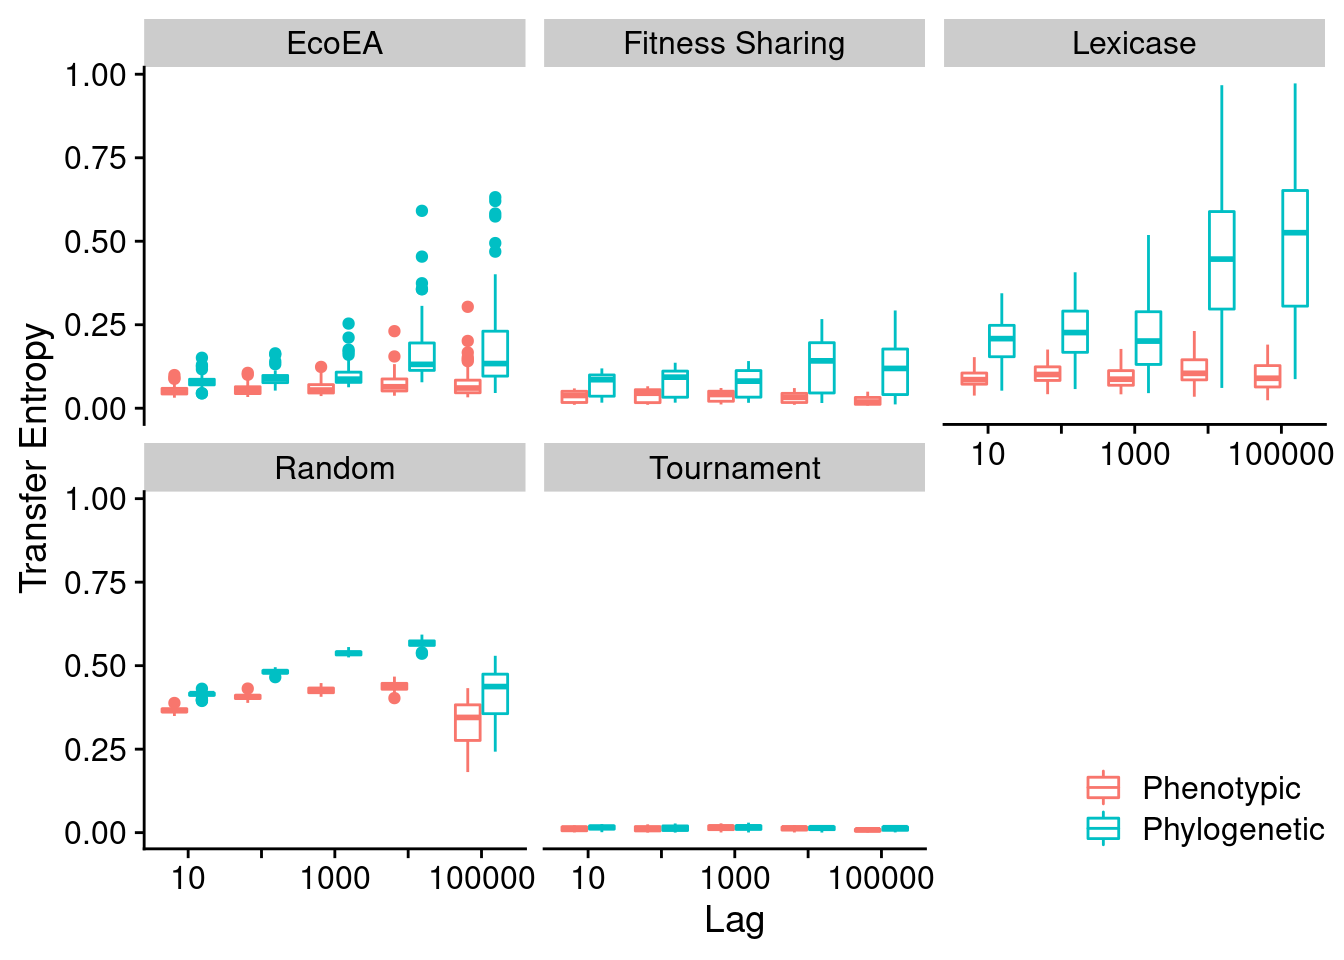
\includegraphics{phylodiversity-in-EC-supplement_files/figure-latex/information_theory_mpd-1.pdf}

\hypertarget{mean-pairwise-distance-vs.shannon-entropy}{%
\subsubsection{Mean pairwise distance vs.~shannon entropy}\label{mean-pairwise-distance-vs.shannon-entropy}}

\begin{Shaded}
\begin{Highlighting}[]
\CommentTok{# Calculate transfer entropy for mean pairwise distance}
\CommentTok{# Time points are 10 generations, so calculating lag 1 gives us lag 10}
\NormalTok{res <-}\StringTok{ }\NormalTok{data }\OperatorTok\StringTok{ }\KeywordTok{group_by}\NormalTok{(directory, selection_name) }\OperatorTok
\KeywordTok{summarise}\NormalTok{(}
  \DataTypeTok{fit_phylo_10 =}     \KeywordTok{condinformation}\NormalTok{(}\KeywordTok{discretize}\NormalTok{(elite_trait_avg), }\CommentTok{# TE phylo -> fit, lag 10}
                                     \KeywordTok{discretize}\NormalTok{(}\KeywordTok{lag}\NormalTok{(mean_phenotype_pairwise_distance, }\DecValTok{1}\NormalTok{)), }
                                     \KeywordTok{discretize}\NormalTok{(}\KeywordTok{lag}\NormalTok{(elite_trait_avg, }\DecValTok{1}\NormalTok{))),}
  \DataTypeTok{fit_phylo_100 =}    \KeywordTok{condinformation}\NormalTok{(}\KeywordTok{discretize}\NormalTok{(elite_trait_avg), }\CommentTok{# TE phylo -> fit, lag 100}
                                     \KeywordTok{discretize}\NormalTok{(}\KeywordTok{lag}\NormalTok{(mean_phenotype_pairwise_distance, }\DecValTok{10}\NormalTok{)), }
                                     \KeywordTok{discretize}\NormalTok{(}\KeywordTok{lag}\NormalTok{(elite_trait_avg, }\DecValTok{10}\NormalTok{))),}
  \DataTypeTok{fit_phylo_1000 =}   \KeywordTok{condinformation}\NormalTok{(}\KeywordTok{discretize}\NormalTok{(elite_trait_avg), }\CommentTok{# TE phylo -> fit, lag 1000}
                                     \KeywordTok{discretize}\NormalTok{(}\KeywordTok{lag}\NormalTok{(mean_phenotype_pairwise_distance, }\DecValTok{100}\NormalTok{)), }
                                     \KeywordTok{discretize}\NormalTok{(}\KeywordTok{lag}\NormalTok{(elite_trait_avg, }\DecValTok{100}\NormalTok{))),}
  \DataTypeTok{fit_phylo_10000 =}  \KeywordTok{condinformation}\NormalTok{(}\KeywordTok{discretize}\NormalTok{(elite_trait_avg), }\CommentTok{# TE phylo -> fit, lag 10000}
                                     \KeywordTok{discretize}\NormalTok{(}\KeywordTok{lag}\NormalTok{(mean_phenotype_pairwise_distance, }\DecValTok{1000}\NormalTok{)), }
                                     \KeywordTok{discretize}\NormalTok{(}\KeywordTok{lag}\NormalTok{(elite_trait_avg, }\DecValTok{1000}\NormalTok{))),}
  \DataTypeTok{fit_phylo_100000 =} \KeywordTok{condinformation}\NormalTok{(}\KeywordTok{discretize}\NormalTok{(elite_trait_avg), }\CommentTok{# TE phylo -> fit, lag 100000}
                                     \KeywordTok{discretize}\NormalTok{(}\KeywordTok{lag}\NormalTok{(mean_phenotype_pairwise_distance, }\DecValTok{10000}\NormalTok{)), }
                                     \KeywordTok{discretize}\NormalTok{(}\KeywordTok{lag}\NormalTok{(elite_trait_avg, }\DecValTok{10000}\NormalTok{))),  }
  \DataTypeTok{fit_fit_10000 =}    \KeywordTok{condinformation}\NormalTok{(}\KeywordTok{discretize}\NormalTok{(elite_trait_avg), }\CommentTok{# Mutual info btwn. fit and lagged fit}
                                     \KeywordTok{discretize}\NormalTok{(}\KeywordTok{lag}\NormalTok{(elite_trait_avg, }\DecValTok{1000}\NormalTok{)), }
                                     \KeywordTok{discretize}\NormalTok{(}\KeywordTok{lag}\NormalTok{(mean_phenotype_pairwise_distance, }\DecValTok{1000}\NormalTok{))),}
  \DataTypeTok{fit_fit_100000 =}   \KeywordTok{condinformation}\NormalTok{(}\KeywordTok{discretize}\NormalTok{(elite_trait_avg), }\CommentTok{# Mutual info btwn. fit and lagged fit}
                                     \KeywordTok{discretize}\NormalTok{(}\KeywordTok{lag}\NormalTok{(elite_trait_avg, }\DecValTok{10000}\NormalTok{)), }
                                     \KeywordTok{discretize}\NormalTok{(}\KeywordTok{lag}\NormalTok{(mean_phenotype_pairwise_distance, }\DecValTok{10000}\NormalTok{))),  }
  \DataTypeTok{fit_pheno_10 =}     \KeywordTok{condinformation}\NormalTok{(}\KeywordTok{discretize}\NormalTok{(elite_trait_avg), }\CommentTok{# TE pheno -> fit, lag 10}
                                     \KeywordTok{discretize}\NormalTok{(}\KeywordTok{lag}\NormalTok{(phen_diversity, }\DecValTok{1}\NormalTok{)), }
                                     \KeywordTok{discretize}\NormalTok{(}\KeywordTok{lag}\NormalTok{(elite_trait_avg, }\DecValTok{1}\NormalTok{))),}
  \DataTypeTok{fit_pheno_100 =}    \KeywordTok{condinformation}\NormalTok{(}\KeywordTok{discretize}\NormalTok{(elite_trait_avg),  }\CommentTok{# TE pheno -> fit, lag 100 }
                                     \KeywordTok{discretize}\NormalTok{(}\KeywordTok{lag}\NormalTok{(phen_diversity, }\DecValTok{10}\NormalTok{)), }
                                     \KeywordTok{discretize}\NormalTok{(}\KeywordTok{lag}\NormalTok{(elite_trait_avg, }\DecValTok{10}\NormalTok{))),}
  \DataTypeTok{fit_pheno_1000 =}   \KeywordTok{condinformation}\NormalTok{(}\KeywordTok{discretize}\NormalTok{(elite_trait_avg),  }\CommentTok{# TE pheno -> fit, lag 1000}
                                     \KeywordTok{discretize}\NormalTok{(}\KeywordTok{lag}\NormalTok{(phen_diversity, }\DecValTok{100}\NormalTok{)), }
                                     \KeywordTok{discretize}\NormalTok{(}\KeywordTok{lag}\NormalTok{(elite_trait_avg, }\DecValTok{100}\NormalTok{))),}
  \DataTypeTok{fit_pheno_10000 =}  \KeywordTok{condinformation}\NormalTok{(}\KeywordTok{discretize}\NormalTok{(elite_trait_avg),  }\CommentTok{# TE pheno -> fit, lag 10000}
                                     \KeywordTok{discretize}\NormalTok{(}\KeywordTok{lag}\NormalTok{(phen_diversity, }\DecValTok{1000}\NormalTok{)), }
                                     \KeywordTok{discretize}\NormalTok{(}\KeywordTok{lag}\NormalTok{(elite_trait_avg, }\DecValTok{1000}\NormalTok{))),}
  \DataTypeTok{fit_pheno_100000 =} \KeywordTok{condinformation}\NormalTok{(}\KeywordTok{discretize}\NormalTok{(elite_trait_avg),  }\CommentTok{# TE pheno -> fit, lag 100000}
                                     \KeywordTok{discretize}\NormalTok{(}\KeywordTok{lag}\NormalTok{(phen_diversity, }\DecValTok{10000}\NormalTok{)), }
                                     \KeywordTok{discretize}\NormalTok{(}\KeywordTok{lag}\NormalTok{(elite_trait_avg, }\DecValTok{10000}\NormalTok{)))}
\NormalTok{)}

\CommentTok{# Turn Transfer Entropy columns into rows}
\NormalTok{res <-}\StringTok{ }\NormalTok{res }\OperatorTok\StringTok{ }\KeywordTok{pivot_longer}\NormalTok{(}\DataTypeTok{cols=}\KeywordTok{contains}\NormalTok{(}\StringTok{"o_10"}\NormalTok{))}
\CommentTok{# Pull lag into a column}
\NormalTok{res}\OperatorTok{$}\NormalTok{offset <-}\StringTok{ }\KeywordTok{str_extract}\NormalTok{(res}\OperatorTok{$}\NormalTok{name, }\StringTok{"[:digit:]*$"}\NormalTok{)}
\CommentTok{# Make column indicating direction of transfer entropy}
\NormalTok{res}\OperatorTok{$}\NormalTok{Type <-}\StringTok{ }\KeywordTok{case_when}\NormalTok{(}\KeywordTok{str_detect}\NormalTok{(res}\OperatorTok{$}\NormalTok{name, }\StringTok{"phylo"}\NormalTok{) }\OperatorTok{~}\StringTok{ "Phylogenetic"}\NormalTok{, }\OtherTok{TRUE} \OperatorTok{~}\StringTok{ "Phenotypic"}\NormalTok{)}

\CommentTok{# Plot transfer entropy}
\KeywordTok{ggplot}\NormalTok{(}
\NormalTok{  res }\OperatorTok\StringTok{ }\KeywordTok{filter}\NormalTok{(}\KeywordTok{str_detect}\NormalTok{(name, }\StringTok{"fit_ph*"}\NormalTok{)), }
  \KeywordTok{aes}\NormalTok{(}
    \DataTypeTok{x=}\KeywordTok{as.factor}\NormalTok{(offset), }
    \DataTypeTok{y=}\NormalTok{value, }
    \DataTypeTok{color=}\NormalTok{Type}
\NormalTok{    )}
\NormalTok{  ) }\OperatorTok{+}\StringTok{ }
\StringTok{  }\KeywordTok{geom_boxplot}\NormalTok{() }\OperatorTok{+}\StringTok{ }
\StringTok{  }\KeywordTok{facet_wrap}\NormalTok{(}\OperatorTok{~}\NormalTok{selection_name) }\OperatorTok{+}\StringTok{ }
\StringTok{  }\KeywordTok{scale_x_discrete}\NormalTok{(}\StringTok{"Lag"}\NormalTok{,}\DataTypeTok{labels=}\KeywordTok{c}\NormalTok{(}\StringTok{"10"}\NormalTok{,}\StringTok{""}\NormalTok{,}\StringTok{"1000"}\NormalTok{,}\StringTok{""}\NormalTok{,}\StringTok{"100000"}\NormalTok{)) }\OperatorTok{+}\StringTok{ }
\StringTok{  }\KeywordTok{scale_y_continuous}\NormalTok{(}\StringTok{"Transfer Entropy"}\NormalTok{) }\OperatorTok{+}\StringTok{ }
\StringTok{  }\KeywordTok{theme}\NormalTok{(}\DataTypeTok{legend.position =} \KeywordTok{c}\NormalTok{(}\DecValTok{1}\NormalTok{, }\DecValTok{0}\NormalTok{),}
        \DataTypeTok{legend.justification =} \KeywordTok{c}\NormalTok{(}\DecValTok{1}\NormalTok{, }\DecValTok{0}\NormalTok{)) }\OperatorTok{+}\StringTok{ }
\StringTok{  }\KeywordTok{scale_color_discrete}\NormalTok{(}\StringTok{""}\NormalTok{)}
\end{Highlighting}
\end{Shaded}

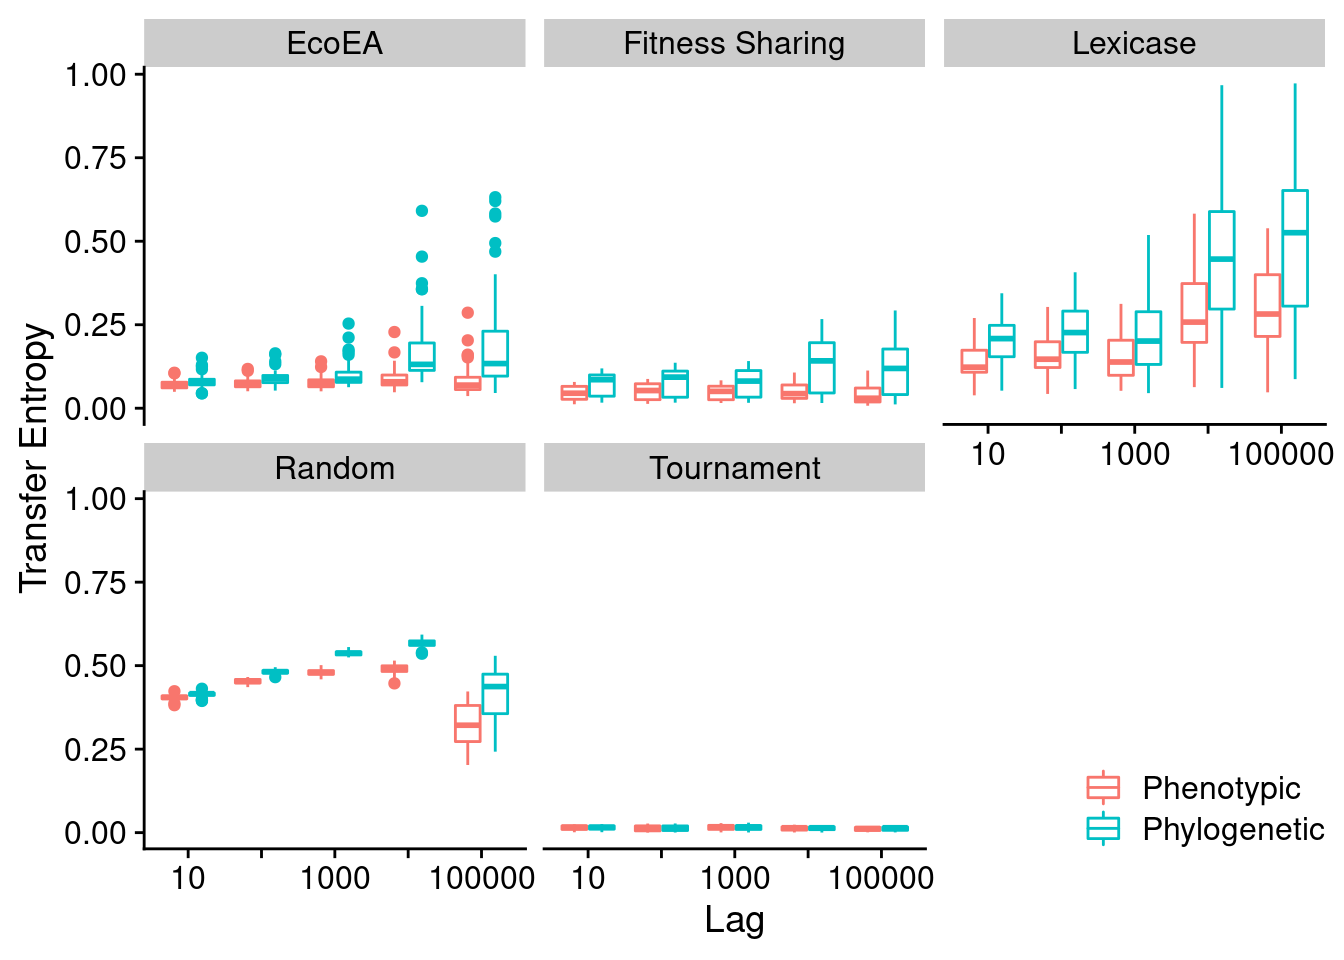
\includegraphics{phylodiversity-in-EC-supplement_files/figure-latex/information_theory_mpd_shannon-1.pdf}

\hypertarget{mean-evolutionary-distinctiveness-vs.phenotypic-richness}{%
\subsubsection{Mean evolutionary distinctiveness vs.~phenotypic richness}\label{mean-evolutionary-distinctiveness-vs.phenotypic-richness}}

\begin{Shaded}
\begin{Highlighting}[]
\CommentTok{# Calculate transfer entropy for mean evolutionary distinctiveness}
\CommentTok{# Time points are 10 generations, so calculating lag 1 gives us lag 10}
\NormalTok{res <-}\StringTok{ }\NormalTok{data }\OperatorTok\StringTok{ }\KeywordTok{group_by}\NormalTok{(directory, selection_name) }\OperatorTok
\KeywordTok{summarise}\NormalTok{(}
  \DataTypeTok{fit_phylo_10 =}     \KeywordTok{condinformation}\NormalTok{(}\KeywordTok{discretize}\NormalTok{(elite_trait_avg), }\CommentTok{# TE phylo -> fit, lag 10}
                                     \KeywordTok{discretize}\NormalTok{(}\KeywordTok{lag}\NormalTok{(mean_phenotype_evolutionary_distinctiveness, }\DecValTok{1}\NormalTok{)), }
                                     \KeywordTok{discretize}\NormalTok{(}\KeywordTok{lag}\NormalTok{(elite_trait_avg, }\DecValTok{1}\NormalTok{))),}
  \DataTypeTok{fit_phylo_100 =}    \KeywordTok{condinformation}\NormalTok{(}\KeywordTok{discretize}\NormalTok{(elite_trait_avg), }\CommentTok{# TE phylo -> fit, lag 100}
                                     \KeywordTok{discretize}\NormalTok{(}\KeywordTok{lag}\NormalTok{(mean_phenotype_evolutionary_distinctiveness, }\DecValTok{10}\NormalTok{)), }
                                     \KeywordTok{discretize}\NormalTok{(}\KeywordTok{lag}\NormalTok{(elite_trait_avg, }\DecValTok{10}\NormalTok{))),}
  \DataTypeTok{fit_phylo_1000 =}   \KeywordTok{condinformation}\NormalTok{(}\KeywordTok{discretize}\NormalTok{(elite_trait_avg), }\CommentTok{# TE phylo -> fit, lag 1000}
                                     \KeywordTok{discretize}\NormalTok{(}\KeywordTok{lag}\NormalTok{(mean_phenotype_evolutionary_distinctiveness, }\DecValTok{100}\NormalTok{)), }
                                     \KeywordTok{discretize}\NormalTok{(}\KeywordTok{lag}\NormalTok{(elite_trait_avg, }\DecValTok{100}\NormalTok{))),}
  \DataTypeTok{fit_phylo_10000 =}  \KeywordTok{condinformation}\NormalTok{(}\KeywordTok{discretize}\NormalTok{(elite_trait_avg), }\CommentTok{# TE phylo -> fit, lag 10000}
                                     \KeywordTok{discretize}\NormalTok{(}\KeywordTok{lag}\NormalTok{(mean_phenotype_evolutionary_distinctiveness, }\DecValTok{1000}\NormalTok{)), }
                                     \KeywordTok{discretize}\NormalTok{(}\KeywordTok{lag}\NormalTok{(elite_trait_avg, }\DecValTok{1000}\NormalTok{))),}
  \DataTypeTok{fit_phylo_100000 =} \KeywordTok{condinformation}\NormalTok{(}\KeywordTok{discretize}\NormalTok{(elite_trait_avg), }\CommentTok{# TE phylo -> fit, lag 100000}
                                     \KeywordTok{discretize}\NormalTok{(}\KeywordTok{lag}\NormalTok{(mean_phenotype_evolutionary_distinctiveness, }\DecValTok{10000}\NormalTok{)), }
                                     \KeywordTok{discretize}\NormalTok{(}\KeywordTok{lag}\NormalTok{(elite_trait_avg, }\DecValTok{10000}\NormalTok{))),  }
  \DataTypeTok{fit_fit_10000 =}    \KeywordTok{condinformation}\NormalTok{(}\KeywordTok{discretize}\NormalTok{(elite_trait_avg), }\CommentTok{# Mutual info btwn. fit and lagged fit}
                                     \KeywordTok{discretize}\NormalTok{(}\KeywordTok{lag}\NormalTok{(elite_trait_avg, }\DecValTok{1000}\NormalTok{)), }
                                     \KeywordTok{discretize}\NormalTok{(}\KeywordTok{lag}\NormalTok{(mean_phenotype_evolutionary_distinctiveness, }\DecValTok{1000}\NormalTok{))),}
  \DataTypeTok{fit_fit_100000 =}   \KeywordTok{condinformation}\NormalTok{(}\KeywordTok{discretize}\NormalTok{(elite_trait_avg), }\CommentTok{# Mutual info btwn. fit and lagged fit}
                                     \KeywordTok{discretize}\NormalTok{(}\KeywordTok{lag}\NormalTok{(elite_trait_avg, }\DecValTok{10000}\NormalTok{)), }
                                     \KeywordTok{discretize}\NormalTok{(}\KeywordTok{lag}\NormalTok{(mean_phenotype_evolutionary_distinctiveness, }\DecValTok{10000}\NormalTok{))),  }
  \DataTypeTok{fit_pheno_10 =}     \KeywordTok{condinformation}\NormalTok{(}\KeywordTok{discretize}\NormalTok{(elite_trait_avg), }\CommentTok{# TE pheno -> fit, lag 10}
                                     \KeywordTok{discretize}\NormalTok{(}\KeywordTok{lag}\NormalTok{(phen_num_taxa, }\DecValTok{1}\NormalTok{)), }
                                     \KeywordTok{discretize}\NormalTok{(}\KeywordTok{lag}\NormalTok{(elite_trait_avg, }\DecValTok{1}\NormalTok{))),}
  \DataTypeTok{fit_pheno_100 =}    \KeywordTok{condinformation}\NormalTok{(}\KeywordTok{discretize}\NormalTok{(elite_trait_avg),  }\CommentTok{# TE pheno -> fit, lag 100 }
                                     \KeywordTok{discretize}\NormalTok{(}\KeywordTok{lag}\NormalTok{(phen_num_taxa, }\DecValTok{10}\NormalTok{)), }
                                     \KeywordTok{discretize}\NormalTok{(}\KeywordTok{lag}\NormalTok{(elite_trait_avg, }\DecValTok{10}\NormalTok{))),}
  \DataTypeTok{fit_pheno_1000 =}   \KeywordTok{condinformation}\NormalTok{(}\KeywordTok{discretize}\NormalTok{(elite_trait_avg),  }\CommentTok{# TE pheno -> fit, lag 1000}
                                     \KeywordTok{discretize}\NormalTok{(}\KeywordTok{lag}\NormalTok{(phen_num_taxa, }\DecValTok{100}\NormalTok{)), }
                                     \KeywordTok{discretize}\NormalTok{(}\KeywordTok{lag}\NormalTok{(elite_trait_avg, }\DecValTok{100}\NormalTok{))),}
  \DataTypeTok{fit_pheno_10000 =}  \KeywordTok{condinformation}\NormalTok{(}\KeywordTok{discretize}\NormalTok{(elite_trait_avg),  }\CommentTok{# TE pheno -> fit, lag 10000}
                                     \KeywordTok{discretize}\NormalTok{(}\KeywordTok{lag}\NormalTok{(phen_num_taxa, }\DecValTok{1000}\NormalTok{)), }
                                     \KeywordTok{discretize}\NormalTok{(}\KeywordTok{lag}\NormalTok{(elite_trait_avg, }\DecValTok{1000}\NormalTok{))),}
  \DataTypeTok{fit_pheno_100000 =} \KeywordTok{condinformation}\NormalTok{(}\KeywordTok{discretize}\NormalTok{(elite_trait_avg),  }\CommentTok{# TE pheno -> fit, lag 100000}
                                     \KeywordTok{discretize}\NormalTok{(}\KeywordTok{lag}\NormalTok{(phen_num_taxa, }\DecValTok{10000}\NormalTok{)), }
                                     \KeywordTok{discretize}\NormalTok{(}\KeywordTok{lag}\NormalTok{(elite_trait_avg, }\DecValTok{10000}\NormalTok{)))}
\NormalTok{)}

\CommentTok{# Turn Transfer Entropy columns into rows}
\NormalTok{res <-}\StringTok{ }\NormalTok{res }\OperatorTok\StringTok{ }\KeywordTok{pivot_longer}\NormalTok{(}\DataTypeTok{cols=}\KeywordTok{contains}\NormalTok{(}\StringTok{"o_10"}\NormalTok{))}
\CommentTok{# Pull lag into a column}
\NormalTok{res}\OperatorTok{$}\NormalTok{offset <-}\StringTok{ }\KeywordTok{str_extract}\NormalTok{(res}\OperatorTok{$}\NormalTok{name, }\StringTok{"[:digit:]*$"}\NormalTok{)}
\CommentTok{# Make column indicating direction of transfer entropy}
\NormalTok{res}\OperatorTok{$}\NormalTok{Type <-}\StringTok{ }\KeywordTok{case_when}\NormalTok{(}\KeywordTok{str_detect}\NormalTok{(res}\OperatorTok{$}\NormalTok{name, }\StringTok{"phylo"}\NormalTok{) }\OperatorTok{~}\StringTok{ "Phylogenetic"}\NormalTok{, }\OtherTok{TRUE} \OperatorTok{~}\StringTok{ "Phenotypic"}\NormalTok{)}

\CommentTok{# Plot transfer entropy}
\KeywordTok{ggplot}\NormalTok{(}
\NormalTok{  res }\OperatorTok\StringTok{ }\KeywordTok{filter}\NormalTok{(}\KeywordTok{str_detect}\NormalTok{(name, }\StringTok{"fit_ph*"}\NormalTok{)), }
  \KeywordTok{aes}\NormalTok{(}
    \DataTypeTok{x=}\KeywordTok{as.factor}\NormalTok{(offset), }
    \DataTypeTok{y=}\NormalTok{value, }
    \DataTypeTok{color=}\NormalTok{Type}
\NormalTok{    )}
\NormalTok{  ) }\OperatorTok{+}\StringTok{ }
\StringTok{  }\KeywordTok{geom_boxplot}\NormalTok{() }\OperatorTok{+}\StringTok{ }
\StringTok{  }\KeywordTok{facet_wrap}\NormalTok{(}\OperatorTok{~}\NormalTok{selection_name) }\OperatorTok{+}\StringTok{ }
\StringTok{  }\KeywordTok{scale_x_discrete}\NormalTok{(}\StringTok{"Lag"}\NormalTok{,}\DataTypeTok{labels=}\KeywordTok{c}\NormalTok{(}\StringTok{"10"}\NormalTok{,}\StringTok{""}\NormalTok{,}\StringTok{"1000"}\NormalTok{,}\StringTok{""}\NormalTok{,}\StringTok{"100000"}\NormalTok{)) }\OperatorTok{+}\StringTok{ }
\StringTok{  }\KeywordTok{scale_y_continuous}\NormalTok{(}\StringTok{"Transfer Entropy"}\NormalTok{) }\OperatorTok{+}\StringTok{ }
\StringTok{  }\KeywordTok{theme}\NormalTok{(}\DataTypeTok{legend.position =} \KeywordTok{c}\NormalTok{(}\DecValTok{1}\NormalTok{, }\DecValTok{0}\NormalTok{),}
        \DataTypeTok{legend.justification =} \KeywordTok{c}\NormalTok{(}\DecValTok{1}\NormalTok{, }\DecValTok{0}\NormalTok{)) }\OperatorTok{+}\StringTok{ }
\StringTok{  }\KeywordTok{scale_color_discrete}\NormalTok{(}\StringTok{""}\NormalTok{)}
\end{Highlighting}
\end{Shaded}

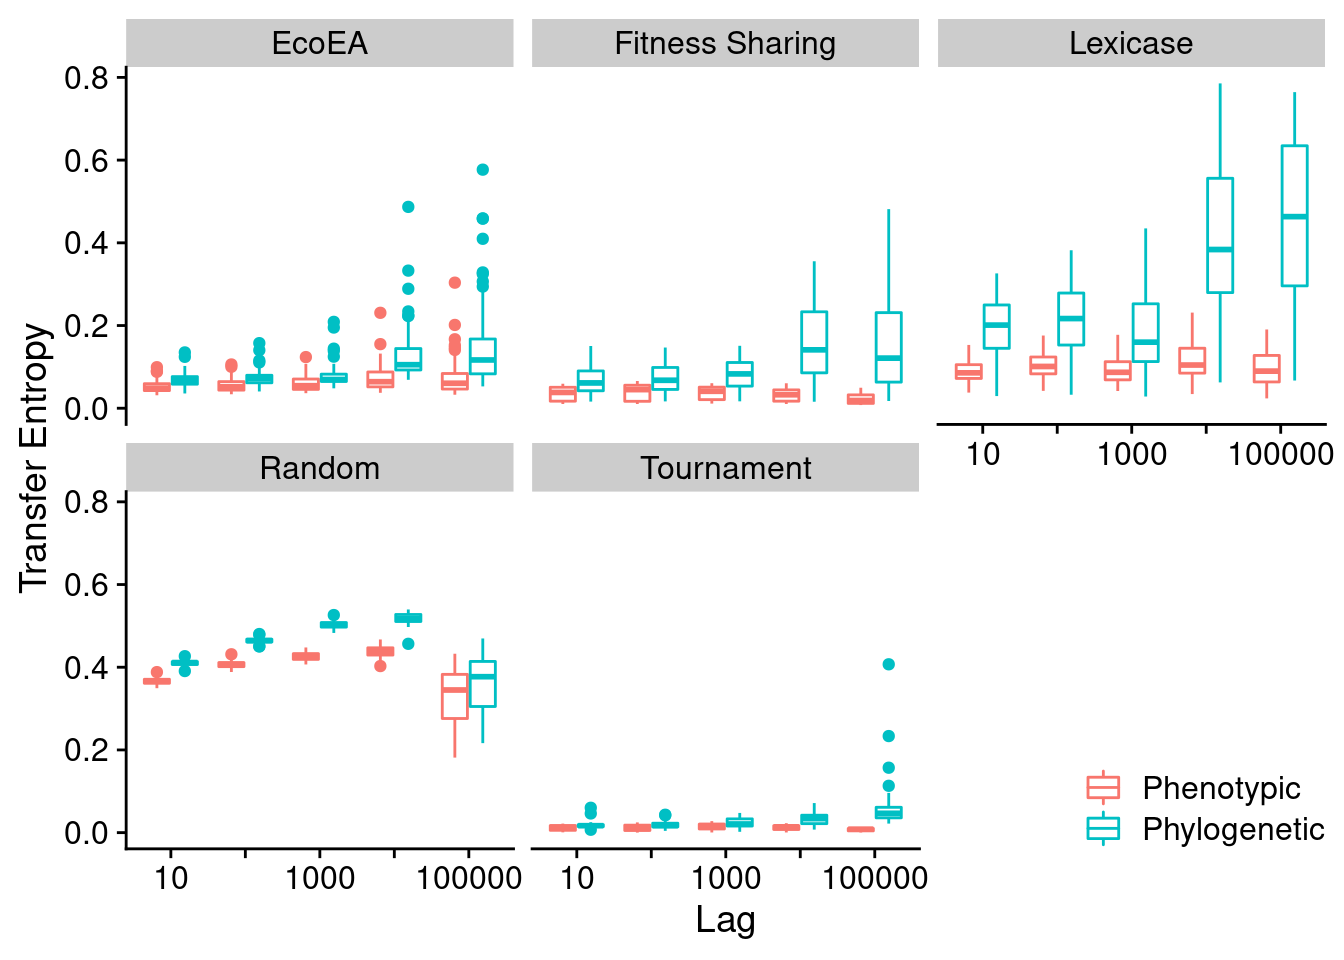
\includegraphics{phylodiversity-in-EC-supplement_files/figure-latex/information_theory_med-1.pdf}

\hypertarget{mean-evolutionary-distinctiveness-vs.shannon-entropy}{%
\subsubsection{Mean evolutionary distinctiveness vs.~shannon entropy}\label{mean-evolutionary-distinctiveness-vs.shannon-entropy}}

\begin{Shaded}
\begin{Highlighting}[]
\CommentTok{# Calculate transfer entropy for mean evolutionary distinctiveness}
\CommentTok{# Time points are 10 generations, so calculating lag 1 gives us lag 10}
\NormalTok{res <-}\StringTok{ }\NormalTok{data }\OperatorTok\StringTok{ }\KeywordTok{group_by}\NormalTok{(directory, selection_name) }\OperatorTok
\KeywordTok{summarise}\NormalTok{(}
  \DataTypeTok{fit_phylo_10 =}     \KeywordTok{condinformation}\NormalTok{(}\KeywordTok{discretize}\NormalTok{(elite_trait_avg), }\CommentTok{# TE phylo -> fit, lag 10}
                                     \KeywordTok{discretize}\NormalTok{(}\KeywordTok{lag}\NormalTok{(mean_phenotype_evolutionary_distinctiveness, }\DecValTok{1}\NormalTok{)), }
                                     \KeywordTok{discretize}\NormalTok{(}\KeywordTok{lag}\NormalTok{(elite_trait_avg, }\DecValTok{1}\NormalTok{))),}
  \DataTypeTok{fit_phylo_100 =}    \KeywordTok{condinformation}\NormalTok{(}\KeywordTok{discretize}\NormalTok{(elite_trait_avg), }\CommentTok{# TE phylo -> fit, lag 100}
                                     \KeywordTok{discretize}\NormalTok{(}\KeywordTok{lag}\NormalTok{(mean_phenotype_evolutionary_distinctiveness, }\DecValTok{10}\NormalTok{)), }
                                     \KeywordTok{discretize}\NormalTok{(}\KeywordTok{lag}\NormalTok{(elite_trait_avg, }\DecValTok{10}\NormalTok{))),}
  \DataTypeTok{fit_phylo_1000 =}   \KeywordTok{condinformation}\NormalTok{(}\KeywordTok{discretize}\NormalTok{(elite_trait_avg), }\CommentTok{# TE phylo -> fit, lag 1000}
                                     \KeywordTok{discretize}\NormalTok{(}\KeywordTok{lag}\NormalTok{(mean_phenotype_evolutionary_distinctiveness, }\DecValTok{100}\NormalTok{)), }
                                     \KeywordTok{discretize}\NormalTok{(}\KeywordTok{lag}\NormalTok{(elite_trait_avg, }\DecValTok{100}\NormalTok{))),}
  \DataTypeTok{fit_phylo_10000 =}  \KeywordTok{condinformation}\NormalTok{(}\KeywordTok{discretize}\NormalTok{(elite_trait_avg), }\CommentTok{# TE phylo -> fit, lag 10000}
                                     \KeywordTok{discretize}\NormalTok{(}\KeywordTok{lag}\NormalTok{(mean_phenotype_evolutionary_distinctiveness, }\DecValTok{1000}\NormalTok{)), }
                                     \KeywordTok{discretize}\NormalTok{(}\KeywordTok{lag}\NormalTok{(elite_trait_avg, }\DecValTok{1000}\NormalTok{))),}
  \DataTypeTok{fit_phylo_100000 =} \KeywordTok{condinformation}\NormalTok{(}\KeywordTok{discretize}\NormalTok{(elite_trait_avg), }\CommentTok{# TE phylo -> fit, lag 100000}
                                     \KeywordTok{discretize}\NormalTok{(}\KeywordTok{lag}\NormalTok{(mean_phenotype_evolutionary_distinctiveness, }\DecValTok{10000}\NormalTok{)), }
                                     \KeywordTok{discretize}\NormalTok{(}\KeywordTok{lag}\NormalTok{(elite_trait_avg, }\DecValTok{10000}\NormalTok{))),  }
  \DataTypeTok{fit_fit_10000 =}    \KeywordTok{condinformation}\NormalTok{(}\KeywordTok{discretize}\NormalTok{(elite_trait_avg), }\CommentTok{# Mutual info btwn. fit and lagged fit}
                                     \KeywordTok{discretize}\NormalTok{(}\KeywordTok{lag}\NormalTok{(elite_trait_avg, }\DecValTok{1000}\NormalTok{)), }
                                     \KeywordTok{discretize}\NormalTok{(}\KeywordTok{lag}\NormalTok{(mean_phenotype_evolutionary_distinctiveness, }\DecValTok{1000}\NormalTok{))),}
  \DataTypeTok{fit_fit_100000 =}   \KeywordTok{condinformation}\NormalTok{(}\KeywordTok{discretize}\NormalTok{(elite_trait_avg), }\CommentTok{# Mutual info btwn. fit and lagged fit}
                                     \KeywordTok{discretize}\NormalTok{(}\KeywordTok{lag}\NormalTok{(elite_trait_avg, }\DecValTok{10000}\NormalTok{)), }
                                     \KeywordTok{discretize}\NormalTok{(}\KeywordTok{lag}\NormalTok{(mean_phenotype_evolutionary_distinctiveness, }\DecValTok{10000}\NormalTok{))),  }
  \DataTypeTok{fit_pheno_10 =}     \KeywordTok{condinformation}\NormalTok{(}\KeywordTok{discretize}\NormalTok{(elite_trait_avg), }\CommentTok{# TE pheno -> fit, lag 10}
                                     \KeywordTok{discretize}\NormalTok{(}\KeywordTok{lag}\NormalTok{(phen_diversity, }\DecValTok{1}\NormalTok{)), }
                                     \KeywordTok{discretize}\NormalTok{(}\KeywordTok{lag}\NormalTok{(elite_trait_avg, }\DecValTok{1}\NormalTok{))),}
  \DataTypeTok{fit_pheno_100 =}    \KeywordTok{condinformation}\NormalTok{(}\KeywordTok{discretize}\NormalTok{(elite_trait_avg),  }\CommentTok{# TE pheno -> fit, lag 100 }
                                     \KeywordTok{discretize}\NormalTok{(}\KeywordTok{lag}\NormalTok{(phen_diversity, }\DecValTok{10}\NormalTok{)), }
                                     \KeywordTok{discretize}\NormalTok{(}\KeywordTok{lag}\NormalTok{(elite_trait_avg, }\DecValTok{10}\NormalTok{))),}
  \DataTypeTok{fit_pheno_1000 =}   \KeywordTok{condinformation}\NormalTok{(}\KeywordTok{discretize}\NormalTok{(elite_trait_avg),  }\CommentTok{# TE pheno -> fit, lag 1000}
                                     \KeywordTok{discretize}\NormalTok{(}\KeywordTok{lag}\NormalTok{(phen_diversity, }\DecValTok{100}\NormalTok{)), }
                                     \KeywordTok{discretize}\NormalTok{(}\KeywordTok{lag}\NormalTok{(elite_trait_avg, }\DecValTok{100}\NormalTok{))),}
  \DataTypeTok{fit_pheno_10000 =}  \KeywordTok{condinformation}\NormalTok{(}\KeywordTok{discretize}\NormalTok{(elite_trait_avg),  }\CommentTok{# TE pheno -> fit, lag 10000}
                                     \KeywordTok{discretize}\NormalTok{(}\KeywordTok{lag}\NormalTok{(phen_diversity, }\DecValTok{1000}\NormalTok{)), }
                                     \KeywordTok{discretize}\NormalTok{(}\KeywordTok{lag}\NormalTok{(elite_trait_avg, }\DecValTok{1000}\NormalTok{))),}
  \DataTypeTok{fit_pheno_100000 =} \KeywordTok{condinformation}\NormalTok{(}\KeywordTok{discretize}\NormalTok{(elite_trait_avg),  }\CommentTok{# TE pheno -> fit, lag 100000}
                                     \KeywordTok{discretize}\NormalTok{(}\KeywordTok{lag}\NormalTok{(phen_diversity, }\DecValTok{10000}\NormalTok{)), }
                                     \KeywordTok{discretize}\NormalTok{(}\KeywordTok{lag}\NormalTok{(elite_trait_avg, }\DecValTok{10000}\NormalTok{)))}
\NormalTok{)}

\CommentTok{# Turn Transfer Entropy columns into rows}
\NormalTok{res <-}\StringTok{ }\NormalTok{res }\OperatorTok\StringTok{ }\KeywordTok{pivot_longer}\NormalTok{(}\DataTypeTok{cols=}\KeywordTok{contains}\NormalTok{(}\StringTok{"o_10"}\NormalTok{))}
\CommentTok{# Pull lag into a column}
\NormalTok{res}\OperatorTok{$}\NormalTok{offset <-}\StringTok{ }\KeywordTok{str_extract}\NormalTok{(res}\OperatorTok{$}\NormalTok{name, }\StringTok{"[:digit:]*$"}\NormalTok{)}
\CommentTok{# Make column indicating direction of transfer entropy}
\NormalTok{res}\OperatorTok{$}\NormalTok{Type <-}\StringTok{ }\KeywordTok{case_when}\NormalTok{(}\KeywordTok{str_detect}\NormalTok{(res}\OperatorTok{$}\NormalTok{name, }\StringTok{"phylo"}\NormalTok{) }\OperatorTok{~}\StringTok{ "Phylogenetic"}\NormalTok{, }\OtherTok{TRUE} \OperatorTok{~}\StringTok{ "Phenotypic"}\NormalTok{)}

\CommentTok{# Plot transfer entropy}
\KeywordTok{ggplot}\NormalTok{(}
\NormalTok{  res }\OperatorTok\StringTok{ }\KeywordTok{filter}\NormalTok{(}\KeywordTok{str_detect}\NormalTok{(name, }\StringTok{"fit_ph*"}\NormalTok{)), }
  \KeywordTok{aes}\NormalTok{(}
    \DataTypeTok{x=}\KeywordTok{as.factor}\NormalTok{(offset), }
    \DataTypeTok{y=}\NormalTok{value, }
    \DataTypeTok{color=}\NormalTok{Type}
\NormalTok{    )}
\NormalTok{  ) }\OperatorTok{+}\StringTok{ }
\StringTok{  }\KeywordTok{geom_boxplot}\NormalTok{() }\OperatorTok{+}\StringTok{ }
\StringTok{  }\KeywordTok{facet_wrap}\NormalTok{(}\OperatorTok{~}\NormalTok{selection_name) }\OperatorTok{+}\StringTok{ }
\StringTok{  }\KeywordTok{scale_x_discrete}\NormalTok{(}\StringTok{"Lag"}\NormalTok{,}\DataTypeTok{labels=}\KeywordTok{c}\NormalTok{(}\StringTok{"10"}\NormalTok{,}\StringTok{""}\NormalTok{,}\StringTok{"1000"}\NormalTok{,}\StringTok{""}\NormalTok{,}\StringTok{"100000"}\NormalTok{)) }\OperatorTok{+}\StringTok{ }
\StringTok{  }\KeywordTok{scale_y_continuous}\NormalTok{(}\StringTok{"Transfer Entropy"}\NormalTok{) }\OperatorTok{+}\StringTok{ }
\StringTok{  }\KeywordTok{theme}\NormalTok{(}\DataTypeTok{legend.position =} \KeywordTok{c}\NormalTok{(}\DecValTok{1}\NormalTok{, }\DecValTok{0}\NormalTok{),}
        \DataTypeTok{legend.justification =} \KeywordTok{c}\NormalTok{(}\DecValTok{1}\NormalTok{, }\DecValTok{0}\NormalTok{)) }\OperatorTok{+}\StringTok{ }
\StringTok{  }\KeywordTok{scale_color_discrete}\NormalTok{(}\StringTok{""}\NormalTok{)}
\end{Highlighting}
\end{Shaded}

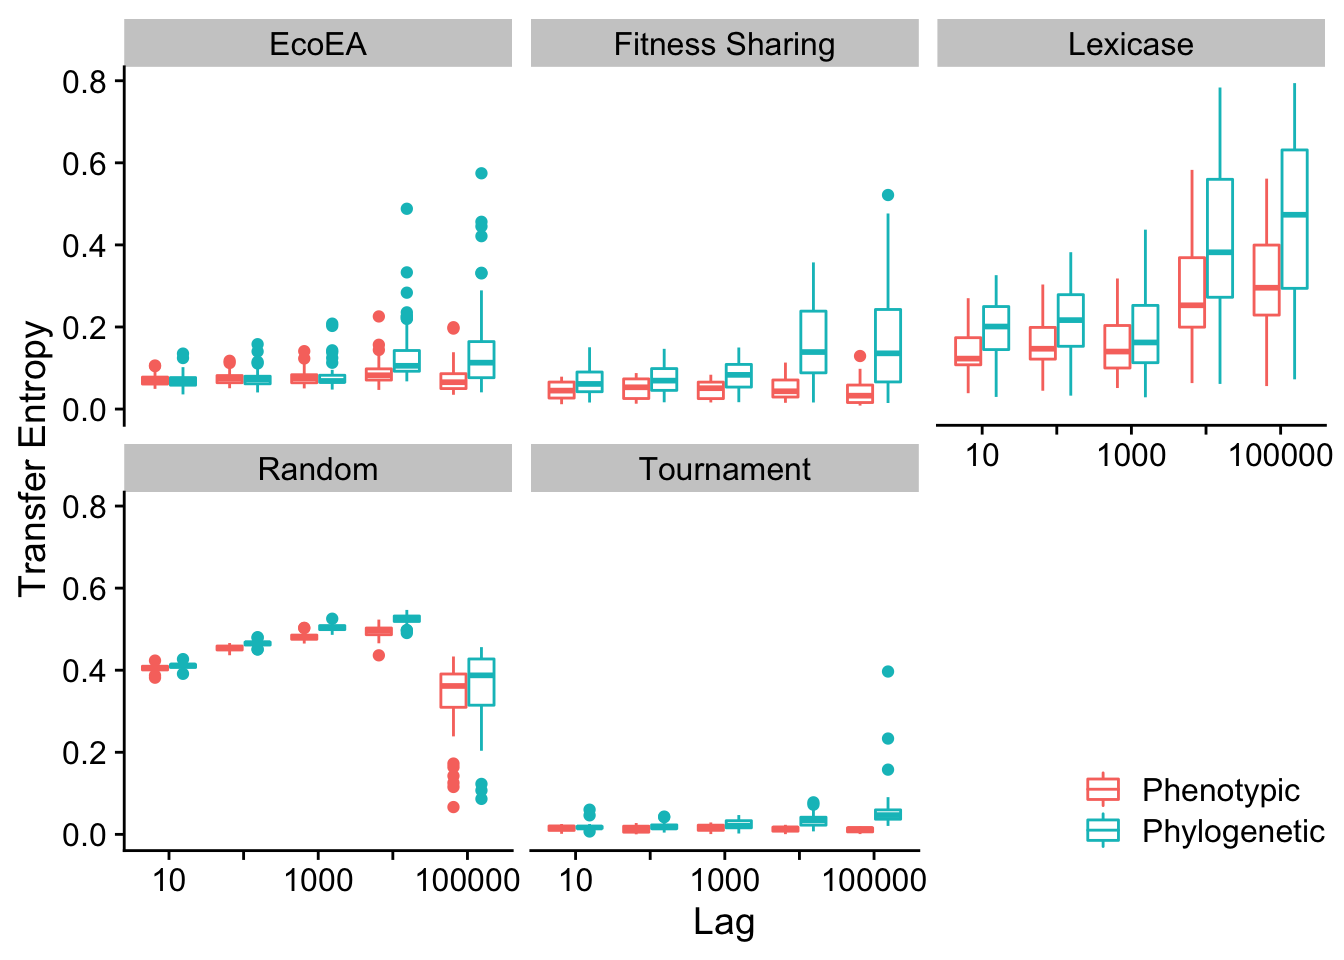
\includegraphics{phylodiversity-in-EC-supplement_files/figure-latex/information_theory_med_shannon-1.pdf}

\hypertarget{transfer-entropy-between-types-of-diversity}{%
\subsection{Transfer entropy between types of diversity}\label{transfer-entropy-between-types-of-diversity}}

\hypertarget{max-pairwise-distance-and-phenotypic-richness}{%
\subsubsection{Max pairwise distance and phenotypic richness}\label{max-pairwise-distance-and-phenotypic-richness}}

\begin{Shaded}
\begin{Highlighting}[]
\NormalTok{res <-}\StringTok{ }\NormalTok{data }\OperatorTok\StringTok{ }\KeywordTok{group_by}\NormalTok{(directory, selection_name) }\OperatorTok
\KeywordTok{summarise}\NormalTok{(}
  \DataTypeTok{phen_phylo_10 =}      \KeywordTok{condinformation}\NormalTok{(}\KeywordTok{discretize}\NormalTok{(phen_num_taxa), }
                                       \KeywordTok{discretize}\NormalTok{(}\KeywordTok{lag}\NormalTok{(max_phenotype_pairwise_distance, }\DecValTok{1}\NormalTok{)), }
                                       \KeywordTok{discretize}\NormalTok{(}\KeywordTok{lag}\NormalTok{(phen_num_taxa, }\DecValTok{1}\NormalTok{))),}
  \DataTypeTok{phen_phylo_100 =}     \KeywordTok{condinformation}\NormalTok{(}\KeywordTok{discretize}\NormalTok{(phen_num_taxa),}
                                       \KeywordTok{discretize}\NormalTok{(}\KeywordTok{lag}\NormalTok{(max_phenotype_pairwise_distance, }\DecValTok{10}\NormalTok{)),}
                                       \KeywordTok{discretize}\NormalTok{(}\KeywordTok{lag}\NormalTok{(phen_num_taxa, }\DecValTok{10}\NormalTok{))),}
  \DataTypeTok{pheno_phylo_1000 =}   \KeywordTok{condinformation}\NormalTok{(}\KeywordTok{discretize}\NormalTok{(phen_num_taxa),}
                                       \KeywordTok{discretize}\NormalTok{(}\KeywordTok{lag}\NormalTok{(max_phenotype_pairwise_distance, }\DecValTok{100}\NormalTok{)),}
                                       \KeywordTok{discretize}\NormalTok{(}\KeywordTok{lag}\NormalTok{(phen_num_taxa, }\DecValTok{100}\NormalTok{))),}
  \DataTypeTok{pheno_phylo_10000 =}  \KeywordTok{condinformation}\NormalTok{(}\KeywordTok{discretize}\NormalTok{(phen_num_taxa),}
                                       \KeywordTok{discretize}\NormalTok{(}\KeywordTok{lag}\NormalTok{(max_phenotype_pairwise_distance, }\DecValTok{1000}\NormalTok{)),}
                                       \KeywordTok{discretize}\NormalTok{(}\KeywordTok{lag}\NormalTok{(phen_num_taxa, }\DecValTok{1000}\NormalTok{))),}
  \DataTypeTok{pheno_phylo_100000 =} \KeywordTok{condinformation}\NormalTok{(}\KeywordTok{discretize}\NormalTok{(phen_num_taxa),}
                                       \KeywordTok{discretize}\NormalTok{(}\KeywordTok{lag}\NormalTok{(max_phenotype_pairwise_distance, }\DecValTok{10000}\NormalTok{)),}
                                       \KeywordTok{discretize}\NormalTok{(}\KeywordTok{lag}\NormalTok{(phen_num_taxa, }\DecValTok{10000}\NormalTok{))),}
  
  \DataTypeTok{phylo_pheno_10 =}     \KeywordTok{condinformation}\NormalTok{(}\KeywordTok{discretize}\NormalTok{(max_phenotype_pairwise_distance),}
                                       \KeywordTok{discretize}\NormalTok{(}\KeywordTok{lag}\NormalTok{(phen_num_taxa, }\DecValTok{1}\NormalTok{)),}
                                       \KeywordTok{discretize}\NormalTok{(}\KeywordTok{lag}\NormalTok{(max_phenotype_pairwise_distance, }\DecValTok{1}\NormalTok{))),}
  \DataTypeTok{phylo_pheno_100 =}    \KeywordTok{condinformation}\NormalTok{(}\KeywordTok{discretize}\NormalTok{(max_phenotype_pairwise_distance),}
                                       \KeywordTok{discretize}\NormalTok{(}\KeywordTok{lag}\NormalTok{(phen_num_taxa, }\DecValTok{10}\NormalTok{)),}
                                       \KeywordTok{discretize}\NormalTok{(}\KeywordTok{lag}\NormalTok{(max_phenotype_pairwise_distance, }\DecValTok{10}\NormalTok{))),}
  \DataTypeTok{phylo_pheno_1000 =}   \KeywordTok{condinformation}\NormalTok{(}\KeywordTok{discretize}\NormalTok{(max_phenotype_pairwise_distance),}
                                       \KeywordTok{discretize}\NormalTok{(}\KeywordTok{lag}\NormalTok{(phen_num_taxa, }\DecValTok{100}\NormalTok{)),}
                                       \KeywordTok{discretize}\NormalTok{(}\KeywordTok{lag}\NormalTok{(max_phenotype_pairwise_distance, }\DecValTok{100}\NormalTok{))),}
  \DataTypeTok{phylo_pheno_10000 =}  \KeywordTok{condinformation}\NormalTok{(}\KeywordTok{discretize}\NormalTok{(max_phenotype_pairwise_distance),}
                                       \KeywordTok{discretize}\NormalTok{(}\KeywordTok{lag}\NormalTok{(phen_num_taxa, }\DecValTok{1000}\NormalTok{)),}
                                       \KeywordTok{discretize}\NormalTok{(}\KeywordTok{lag}\NormalTok{(max_phenotype_pairwise_distance, }\DecValTok{1000}\NormalTok{))),}
  \DataTypeTok{phylo_pheno_100000 =} \KeywordTok{condinformation}\NormalTok{(}\KeywordTok{discretize}\NormalTok{(max_phenotype_pairwise_distance),}
                                       \KeywordTok{discretize}\NormalTok{(}\KeywordTok{lag}\NormalTok{(phen_num_taxa, }\DecValTok{10000}\NormalTok{)),}
                                       \KeywordTok{discretize}\NormalTok{(}\KeywordTok{lag}\NormalTok{(max_phenotype_pairwise_distance, }\DecValTok{10000}\NormalTok{)))}
\NormalTok{)}

\CommentTok{# Turn Transfer Entropy columns into rows}
\NormalTok{res <-}\StringTok{ }\NormalTok{res }\OperatorTok\StringTok{ }\KeywordTok{pivot_longer}\NormalTok{(}\DataTypeTok{cols=}\KeywordTok{contains}\NormalTok{(}\StringTok{"phylo"}\NormalTok{))}
\CommentTok{# Pull lag into a column}
\NormalTok{res}\OperatorTok{$}\NormalTok{offset <-}\StringTok{ }\KeywordTok{str_extract}\NormalTok{(res}\OperatorTok{$}\NormalTok{name, }\StringTok{"[:digit:]*$"}\NormalTok{)}
\CommentTok{# Make column indicating direction of transfer entropy}
\NormalTok{res}\OperatorTok{$}\NormalTok{Type <-}\StringTok{ }\KeywordTok{case_when}\NormalTok{(}\KeywordTok{str_detect}\NormalTok{(res}\OperatorTok{$}\NormalTok{name, }\StringTok{"phylo_pheno"}\NormalTok{) }\OperatorTok{~}\StringTok{ "}\CharTok{\textbackslash{}n}\StringTok{Phenotypic}\CharTok{\textbackslash{}n\textbackslash{}t}\StringTok{->}\CharTok{\textbackslash{}n}\StringTok{Phylogenetic}\CharTok{\textbackslash{}n}\StringTok{"}\NormalTok{, }\OtherTok{TRUE} \OperatorTok{~}\StringTok{ "}\CharTok{\textbackslash{}n}\StringTok{Phylogenetic}\CharTok{\textbackslash{}n\textbackslash{}t}\StringTok{->}\CharTok{\textbackslash{}n}\StringTok{Phenotypic}\CharTok{\textbackslash{}n}\StringTok{"}\NormalTok{)}

\KeywordTok{ggplot}\NormalTok{(}
\NormalTok{  res, }
  \KeywordTok{aes}\NormalTok{(}
    \DataTypeTok{x=}\KeywordTok{as.factor}\NormalTok{(offset), }
    \DataTypeTok{y=}\NormalTok{value, }
    \DataTypeTok{color=}\NormalTok{Type}
\NormalTok{    )}
\NormalTok{  ) }\OperatorTok{+}\StringTok{ }
\StringTok{  }\KeywordTok{geom_boxplot}\NormalTok{() }\OperatorTok{+}\StringTok{ }
\StringTok{  }\KeywordTok{facet_wrap}\NormalTok{(}\OperatorTok{~}\NormalTok{selection_name) }\OperatorTok{+}\StringTok{ }
\StringTok{  }\KeywordTok{scale_x_discrete}\NormalTok{(}\StringTok{"Lag"}\NormalTok{,}\DataTypeTok{labels=}\KeywordTok{c}\NormalTok{(}\StringTok{"10"}\NormalTok{,}\StringTok{""}\NormalTok{,}\StringTok{"1000"}\NormalTok{,}\StringTok{""}\NormalTok{,}\StringTok{"100000"}\NormalTok{)) }\OperatorTok{+}\StringTok{ }
\StringTok{  }\KeywordTok{scale_y_continuous}\NormalTok{(}\StringTok{"Transfer Entropy"}\NormalTok{) }\OperatorTok{+}\StringTok{ }
\StringTok{  }\KeywordTok{theme}\NormalTok{(}\DataTypeTok{legend.position =} \KeywordTok{c}\NormalTok{(}\DecValTok{1}\NormalTok{, }\DecValTok{0}\NormalTok{),}
        \DataTypeTok{legend.justification =} \KeywordTok{c}\NormalTok{(}\DecValTok{1}\NormalTok{, }\DecValTok{0}\NormalTok{)) }\OperatorTok{+}\StringTok{ }
\StringTok{  }\KeywordTok{scale_color_discrete}\NormalTok{(}\StringTok{""}\NormalTok{)}
\end{Highlighting}
\end{Shaded}

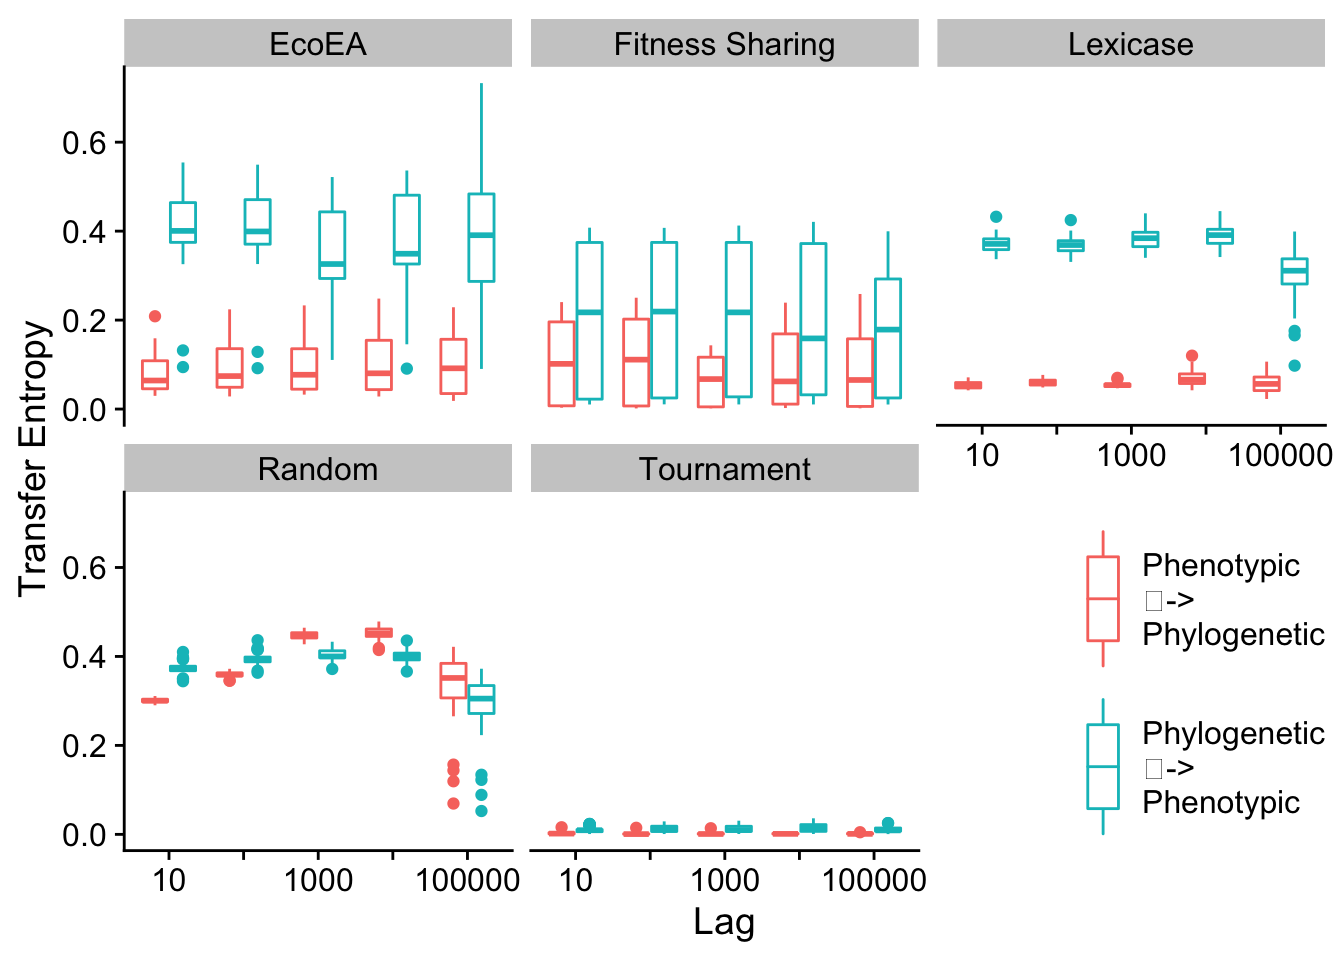
\includegraphics{phylodiversity-in-EC-supplement_files/figure-latex/information_theory_pheno_phylo-1.pdf}

\hypertarget{mean-pairwise-distance-and-phenotypic-richness}{%
\subsubsection{Mean pairwise distance and phenotypic richness}\label{mean-pairwise-distance-and-phenotypic-richness}}

\begin{Shaded}
\begin{Highlighting}[]
\NormalTok{res <-}\StringTok{ }\NormalTok{data }\OperatorTok\StringTok{ }\KeywordTok{group_by}\NormalTok{(directory, selection_name) }\OperatorTok
\KeywordTok{summarise}\NormalTok{(}
  \DataTypeTok{phen_phylo_10 =}      \KeywordTok{condinformation}\NormalTok{(}\KeywordTok{discretize}\NormalTok{(phen_num_taxa), }
                                       \KeywordTok{discretize}\NormalTok{(}\KeywordTok{lag}\NormalTok{(mean_phenotype_pairwise_distance, }\DecValTok{1}\NormalTok{)), }
                                       \KeywordTok{discretize}\NormalTok{(}\KeywordTok{lag}\NormalTok{(phen_num_taxa, }\DecValTok{1}\NormalTok{))),}
  \DataTypeTok{phen_phylo_100 =}     \KeywordTok{condinformation}\NormalTok{(}\KeywordTok{discretize}\NormalTok{(phen_num_taxa),}
                                       \KeywordTok{discretize}\NormalTok{(}\KeywordTok{lag}\NormalTok{(mean_phenotype_pairwise_distance, }\DecValTok{10}\NormalTok{)),}
                                       \KeywordTok{discretize}\NormalTok{(}\KeywordTok{lag}\NormalTok{(phen_num_taxa, }\DecValTok{10}\NormalTok{))),}
  \DataTypeTok{pheno_phylo_1000 =}   \KeywordTok{condinformation}\NormalTok{(}\KeywordTok{discretize}\NormalTok{(phen_num_taxa),}
                                       \KeywordTok{discretize}\NormalTok{(}\KeywordTok{lag}\NormalTok{(mean_phenotype_pairwise_distance, }\DecValTok{100}\NormalTok{)),}
                                       \KeywordTok{discretize}\NormalTok{(}\KeywordTok{lag}\NormalTok{(phen_num_taxa, }\DecValTok{100}\NormalTok{))),}
  \DataTypeTok{pheno_phylo_10000 =}  \KeywordTok{condinformation}\NormalTok{(}\KeywordTok{discretize}\NormalTok{(phen_num_taxa),}
                                       \KeywordTok{discretize}\NormalTok{(}\KeywordTok{lag}\NormalTok{(mean_phenotype_pairwise_distance, }\DecValTok{1000}\NormalTok{)),}
                                       \KeywordTok{discretize}\NormalTok{(}\KeywordTok{lag}\NormalTok{(phen_num_taxa, }\DecValTok{1000}\NormalTok{))),}
  \DataTypeTok{pheno_phylo_100000 =} \KeywordTok{condinformation}\NormalTok{(}\KeywordTok{discretize}\NormalTok{(phen_num_taxa),}
                                       \KeywordTok{discretize}\NormalTok{(}\KeywordTok{lag}\NormalTok{(mean_phenotype_pairwise_distance, }\DecValTok{10000}\NormalTok{)),}
                                       \KeywordTok{discretize}\NormalTok{(}\KeywordTok{lag}\NormalTok{(phen_num_taxa, }\DecValTok{10000}\NormalTok{))),}
  
  \DataTypeTok{phylo_pheno_10 =}     \KeywordTok{condinformation}\NormalTok{(}\KeywordTok{discretize}\NormalTok{(mean_phenotype_pairwise_distance),}
                                       \KeywordTok{discretize}\NormalTok{(}\KeywordTok{lag}\NormalTok{(phen_num_taxa, }\DecValTok{1}\NormalTok{)),}
                                       \KeywordTok{discretize}\NormalTok{(}\KeywordTok{lag}\NormalTok{(mean_phenotype_pairwise_distance, }\DecValTok{1}\NormalTok{))),}
  \DataTypeTok{phylo_pheno_100 =}    \KeywordTok{condinformation}\NormalTok{(}\KeywordTok{discretize}\NormalTok{(mean_phenotype_pairwise_distance),}
                                       \KeywordTok{discretize}\NormalTok{(}\KeywordTok{lag}\NormalTok{(phen_num_taxa, }\DecValTok{10}\NormalTok{)),}
                                       \KeywordTok{discretize}\NormalTok{(}\KeywordTok{lag}\NormalTok{(mean_phenotype_pairwise_distance, }\DecValTok{10}\NormalTok{))),}
  \DataTypeTok{phylo_pheno_1000 =}   \KeywordTok{condinformation}\NormalTok{(}\KeywordTok{discretize}\NormalTok{(mean_phenotype_pairwise_distance),}
                                       \KeywordTok{discretize}\NormalTok{(}\KeywordTok{lag}\NormalTok{(phen_num_taxa, }\DecValTok{100}\NormalTok{)),}
                                       \KeywordTok{discretize}\NormalTok{(}\KeywordTok{lag}\NormalTok{(mean_phenotype_pairwise_distance, }\DecValTok{100}\NormalTok{))),}
  \DataTypeTok{phylo_pheno_10000 =}  \KeywordTok{condinformation}\NormalTok{(}\KeywordTok{discretize}\NormalTok{(mean_phenotype_pairwise_distance),}
                                       \KeywordTok{discretize}\NormalTok{(}\KeywordTok{lag}\NormalTok{(phen_num_taxa, }\DecValTok{1000}\NormalTok{)),}
                                       \KeywordTok{discretize}\NormalTok{(}\KeywordTok{lag}\NormalTok{(mean_phenotype_pairwise_distance, }\DecValTok{1000}\NormalTok{))),}
  \DataTypeTok{phylo_pheno_100000 =} \KeywordTok{condinformation}\NormalTok{(}\KeywordTok{discretize}\NormalTok{(mean_phenotype_pairwise_distance),}
                                       \KeywordTok{discretize}\NormalTok{(}\KeywordTok{lag}\NormalTok{(phen_num_taxa, }\DecValTok{10000}\NormalTok{)),}
                                       \KeywordTok{discretize}\NormalTok{(}\KeywordTok{lag}\NormalTok{(mean_phenotype_pairwise_distance, }\DecValTok{10000}\NormalTok{)))}
\NormalTok{)}

\CommentTok{# Turn Transfer Entropy columns into rows}
\NormalTok{res <-}\StringTok{ }\NormalTok{res }\OperatorTok\StringTok{ }\KeywordTok{pivot_longer}\NormalTok{(}\DataTypeTok{cols=}\KeywordTok{contains}\NormalTok{(}\StringTok{"phylo"}\NormalTok{))}
\CommentTok{# Pull lag into a column}
\NormalTok{res}\OperatorTok{$}\NormalTok{offset <-}\StringTok{ }\KeywordTok{str_extract}\NormalTok{(res}\OperatorTok{$}\NormalTok{name, }\StringTok{"[:digit:]*$"}\NormalTok{)}
\CommentTok{# Make column indicating direction of transfer entropy}
\NormalTok{res}\OperatorTok{$}\NormalTok{Type <-}\StringTok{ }\KeywordTok{case_when}\NormalTok{(}\KeywordTok{str_detect}\NormalTok{(res}\OperatorTok{$}\NormalTok{name, }\StringTok{"phylo_pheno"}\NormalTok{) }\OperatorTok{~}\StringTok{ "}\CharTok{\textbackslash{}n}\StringTok{Phenotypic}\CharTok{\textbackslash{}n\textbackslash{}t}\StringTok{->}\CharTok{\textbackslash{}n}\StringTok{Phylogenetic}\CharTok{\textbackslash{}n}\StringTok{"}\NormalTok{, }\OtherTok{TRUE} \OperatorTok{~}\StringTok{ "}\CharTok{\textbackslash{}n}\StringTok{Phylogenetic}\CharTok{\textbackslash{}n\textbackslash{}t}\StringTok{->}\CharTok{\textbackslash{}n}\StringTok{Phenotypic}\CharTok{\textbackslash{}n}\StringTok{"}\NormalTok{)}

\KeywordTok{ggplot}\NormalTok{(}
\NormalTok{  res, }
  \KeywordTok{aes}\NormalTok{(}
    \DataTypeTok{x=}\KeywordTok{as.factor}\NormalTok{(offset), }
    \DataTypeTok{y=}\NormalTok{value, }
    \DataTypeTok{color=}\NormalTok{Type}
\NormalTok{    )}
\NormalTok{  ) }\OperatorTok{+}\StringTok{ }
\StringTok{  }\KeywordTok{geom_boxplot}\NormalTok{() }\OperatorTok{+}\StringTok{ }
\StringTok{  }\KeywordTok{facet_wrap}\NormalTok{(}\OperatorTok{~}\NormalTok{selection_name) }\OperatorTok{+}\StringTok{ }
\StringTok{  }\KeywordTok{scale_x_discrete}\NormalTok{(}\StringTok{"Lag"}\NormalTok{,}\DataTypeTok{labels=}\KeywordTok{c}\NormalTok{(}\StringTok{"10"}\NormalTok{,}\StringTok{""}\NormalTok{,}\StringTok{"1000"}\NormalTok{,}\StringTok{""}\NormalTok{,}\StringTok{"100000"}\NormalTok{)) }\OperatorTok{+}\StringTok{ }
\StringTok{  }\KeywordTok{scale_y_continuous}\NormalTok{(}\StringTok{"Transfer Entropy"}\NormalTok{) }\OperatorTok{+}\StringTok{ }
\StringTok{  }\KeywordTok{theme}\NormalTok{(}\DataTypeTok{legend.position =} \KeywordTok{c}\NormalTok{(}\DecValTok{1}\NormalTok{, }\DecValTok{0}\NormalTok{),}
        \DataTypeTok{legend.justification =} \KeywordTok{c}\NormalTok{(}\DecValTok{1}\NormalTok{, }\DecValTok{0}\NormalTok{)) }\OperatorTok{+}\StringTok{ }
\StringTok{  }\KeywordTok{scale_color_discrete}\NormalTok{(}\StringTok{""}\NormalTok{)}
\end{Highlighting}
\end{Shaded}

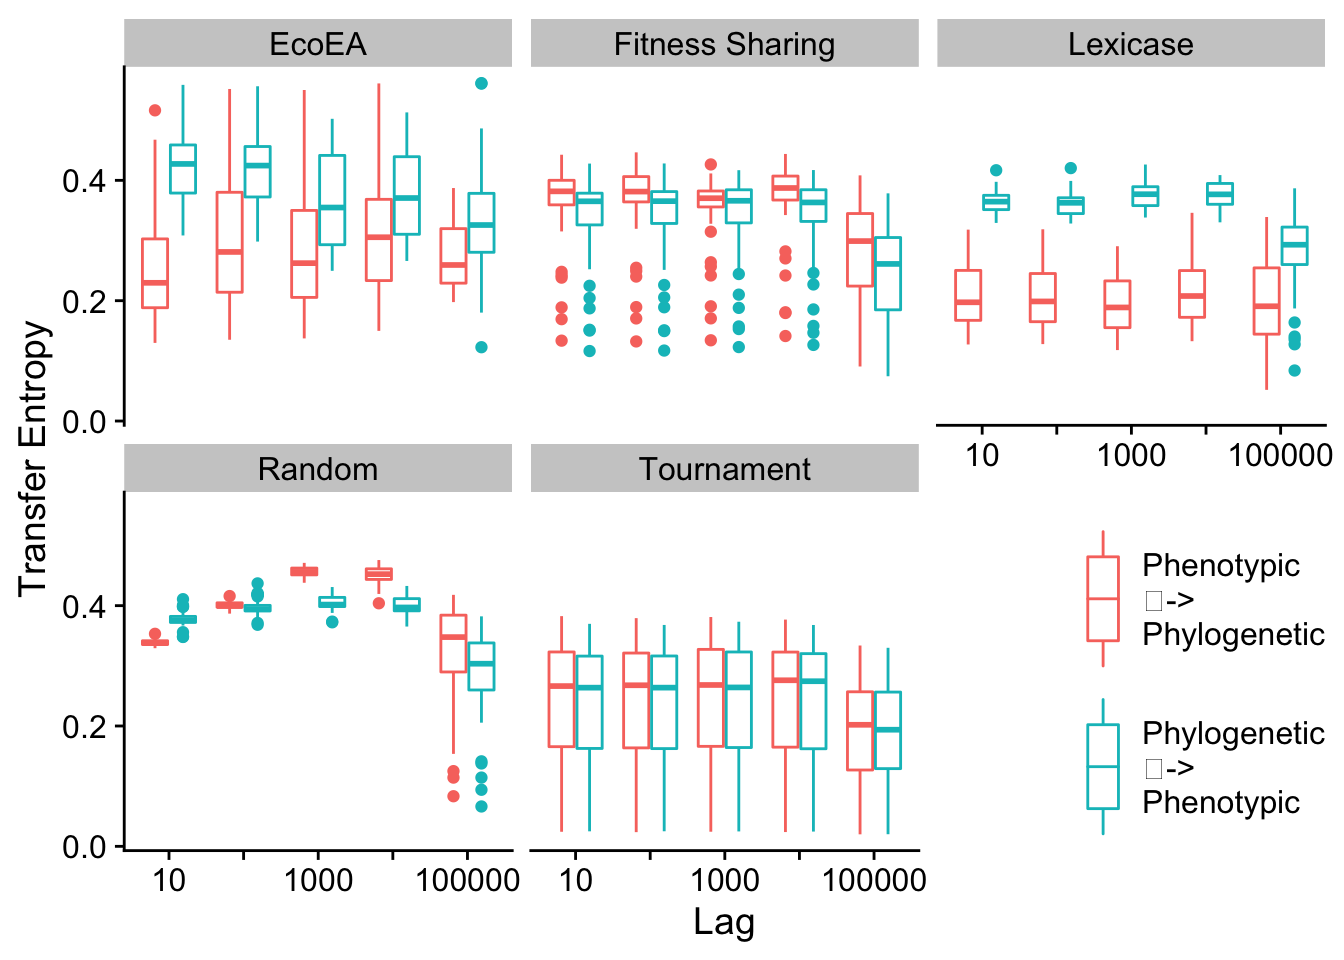
\includegraphics{phylodiversity-in-EC-supplement_files/figure-latex/information_theory_pheno_phylo_mpd-1.pdf}

\hypertarget{mean-pairwise-distance-and-shannon-diversity}{%
\subsubsection{Mean pairwise distance and shannon diversity}\label{mean-pairwise-distance-and-shannon-diversity}}

\begin{Shaded}
\begin{Highlighting}[]
\NormalTok{res <-}\StringTok{ }\NormalTok{data }\OperatorTok\StringTok{ }\KeywordTok{group_by}\NormalTok{(directory, selection_name) }\OperatorTok
\KeywordTok{summarise}\NormalTok{(}
  \DataTypeTok{phen_phylo_10 =}      \KeywordTok{condinformation}\NormalTok{(}\KeywordTok{discretize}\NormalTok{(phen_diversity), }
                                       \KeywordTok{discretize}\NormalTok{(}\KeywordTok{lag}\NormalTok{(mean_phenotype_pairwise_distance, }\DecValTok{1}\NormalTok{)), }
                                       \KeywordTok{discretize}\NormalTok{(}\KeywordTok{lag}\NormalTok{(phen_diversity, }\DecValTok{1}\NormalTok{))),}
  \DataTypeTok{phen_phylo_100 =}     \KeywordTok{condinformation}\NormalTok{(}\KeywordTok{discretize}\NormalTok{(phen_diversity),}
                                       \KeywordTok{discretize}\NormalTok{(}\KeywordTok{lag}\NormalTok{(mean_phenotype_pairwise_distance, }\DecValTok{10}\NormalTok{)),}
                                       \KeywordTok{discretize}\NormalTok{(}\KeywordTok{lag}\NormalTok{(phen_diversity, }\DecValTok{10}\NormalTok{))),}
  \DataTypeTok{pheno_phylo_1000 =}   \KeywordTok{condinformation}\NormalTok{(}\KeywordTok{discretize}\NormalTok{(phen_diversity),}
                                       \KeywordTok{discretize}\NormalTok{(}\KeywordTok{lag}\NormalTok{(mean_phenotype_pairwise_distance, }\DecValTok{100}\NormalTok{)),}
                                       \KeywordTok{discretize}\NormalTok{(}\KeywordTok{lag}\NormalTok{(phen_diversity, }\DecValTok{100}\NormalTok{))),}
  \DataTypeTok{pheno_phylo_10000 =}  \KeywordTok{condinformation}\NormalTok{(}\KeywordTok{discretize}\NormalTok{(phen_diversity),}
                                       \KeywordTok{discretize}\NormalTok{(}\KeywordTok{lag}\NormalTok{(mean_phenotype_pairwise_distance, }\DecValTok{1000}\NormalTok{)),}
                                       \KeywordTok{discretize}\NormalTok{(}\KeywordTok{lag}\NormalTok{(phen_diversity, }\DecValTok{1000}\NormalTok{))),}
  \DataTypeTok{pheno_phylo_100000 =} \KeywordTok{condinformation}\NormalTok{(}\KeywordTok{discretize}\NormalTok{(phen_diversity),}
                                       \KeywordTok{discretize}\NormalTok{(}\KeywordTok{lag}\NormalTok{(mean_phenotype_pairwise_distance, }\DecValTok{10000}\NormalTok{)),}
                                       \KeywordTok{discretize}\NormalTok{(}\KeywordTok{lag}\NormalTok{(phen_diversity, }\DecValTok{10000}\NormalTok{))),}
  
  \DataTypeTok{phylo_pheno_10 =}     \KeywordTok{condinformation}\NormalTok{(}\KeywordTok{discretize}\NormalTok{(mean_phenotype_pairwise_distance),}
                                       \KeywordTok{discretize}\NormalTok{(}\KeywordTok{lag}\NormalTok{(phen_diversity, }\DecValTok{1}\NormalTok{)),}
                                       \KeywordTok{discretize}\NormalTok{(}\KeywordTok{lag}\NormalTok{(mean_phenotype_pairwise_distance, }\DecValTok{1}\NormalTok{))),}
  \DataTypeTok{phylo_pheno_100 =}    \KeywordTok{condinformation}\NormalTok{(}\KeywordTok{discretize}\NormalTok{(mean_phenotype_pairwise_distance),}
                                       \KeywordTok{discretize}\NormalTok{(}\KeywordTok{lag}\NormalTok{(phen_diversity, }\DecValTok{10}\NormalTok{)),}
                                       \KeywordTok{discretize}\NormalTok{(}\KeywordTok{lag}\NormalTok{(mean_phenotype_pairwise_distance, }\DecValTok{10}\NormalTok{))),}
  \DataTypeTok{phylo_pheno_1000 =}   \KeywordTok{condinformation}\NormalTok{(}\KeywordTok{discretize}\NormalTok{(mean_phenotype_pairwise_distance),}
                                       \KeywordTok{discretize}\NormalTok{(}\KeywordTok{lag}\NormalTok{(phen_diversity, }\DecValTok{100}\NormalTok{)),}
                                       \KeywordTok{discretize}\NormalTok{(}\KeywordTok{lag}\NormalTok{(mean_phenotype_pairwise_distance, }\DecValTok{100}\NormalTok{))),}
  \DataTypeTok{phylo_pheno_10000 =}  \KeywordTok{condinformation}\NormalTok{(}\KeywordTok{discretize}\NormalTok{(mean_phenotype_pairwise_distance),}
                                       \KeywordTok{discretize}\NormalTok{(}\KeywordTok{lag}\NormalTok{(phen_diversity, }\DecValTok{1000}\NormalTok{)),}
                                       \KeywordTok{discretize}\NormalTok{(}\KeywordTok{lag}\NormalTok{(mean_phenotype_pairwise_distance, }\DecValTok{1000}\NormalTok{))),}
  \DataTypeTok{phylo_pheno_100000 =} \KeywordTok{condinformation}\NormalTok{(}\KeywordTok{discretize}\NormalTok{(mean_phenotype_pairwise_distance),}
                                       \KeywordTok{discretize}\NormalTok{(}\KeywordTok{lag}\NormalTok{(phen_diversity, }\DecValTok{10000}\NormalTok{)),}
                                       \KeywordTok{discretize}\NormalTok{(}\KeywordTok{lag}\NormalTok{(mean_phenotype_pairwise_distance, }\DecValTok{10000}\NormalTok{)))}
\NormalTok{)}

\CommentTok{# Turn Transfer Entropy columns into rows}
\NormalTok{res <-}\StringTok{ }\NormalTok{res }\OperatorTok\StringTok{ }\KeywordTok{pivot_longer}\NormalTok{(}\DataTypeTok{cols=}\KeywordTok{contains}\NormalTok{(}\StringTok{"phylo"}\NormalTok{))}
\CommentTok{# Pull lag into a column}
\NormalTok{res}\OperatorTok{$}\NormalTok{offset <-}\StringTok{ }\KeywordTok{str_extract}\NormalTok{(res}\OperatorTok{$}\NormalTok{name, }\StringTok{"[:digit:]*$"}\NormalTok{)}
\CommentTok{# Make column indicating direction of transfer entropy}
\NormalTok{res}\OperatorTok{$}\NormalTok{Type <-}\StringTok{ }\KeywordTok{case_when}\NormalTok{(}\KeywordTok{str_detect}\NormalTok{(res}\OperatorTok{$}\NormalTok{name, }\StringTok{"phylo_pheno"}\NormalTok{) }\OperatorTok{~}\StringTok{ "}\CharTok{\textbackslash{}n}\StringTok{Phenotypic}\CharTok{\textbackslash{}n\textbackslash{}t}\StringTok{->}\CharTok{\textbackslash{}n}\StringTok{Phylogenetic}\CharTok{\textbackslash{}n}\StringTok{"}\NormalTok{, }\OtherTok{TRUE} \OperatorTok{~}\StringTok{ "}\CharTok{\textbackslash{}n}\StringTok{Phylogenetic}\CharTok{\textbackslash{}n\textbackslash{}t}\StringTok{->}\CharTok{\textbackslash{}n}\StringTok{Phenotypic}\CharTok{\textbackslash{}n}\StringTok{"}\NormalTok{)}

\KeywordTok{ggplot}\NormalTok{(}
\NormalTok{  res, }
  \KeywordTok{aes}\NormalTok{(}
    \DataTypeTok{x=}\KeywordTok{as.factor}\NormalTok{(offset), }
    \DataTypeTok{y=}\NormalTok{value, }
    \DataTypeTok{color=}\NormalTok{Type}
\NormalTok{    )}
\NormalTok{  ) }\OperatorTok{+}\StringTok{ }
\StringTok{  }\KeywordTok{geom_boxplot}\NormalTok{() }\OperatorTok{+}\StringTok{ }
\StringTok{  }\KeywordTok{facet_wrap}\NormalTok{(}\OperatorTok{~}\NormalTok{selection_name) }\OperatorTok{+}\StringTok{ }
\StringTok{  }\KeywordTok{scale_x_discrete}\NormalTok{(}\StringTok{"Lag"}\NormalTok{,}\DataTypeTok{labels=}\KeywordTok{c}\NormalTok{(}\StringTok{"10"}\NormalTok{,}\StringTok{""}\NormalTok{,}\StringTok{"1000"}\NormalTok{,}\StringTok{""}\NormalTok{,}\StringTok{"100000"}\NormalTok{)) }\OperatorTok{+}\StringTok{ }
\StringTok{  }\KeywordTok{scale_y_continuous}\NormalTok{(}\StringTok{"Transfer Entropy"}\NormalTok{) }\OperatorTok{+}\StringTok{ }
\StringTok{  }\KeywordTok{theme}\NormalTok{(}\DataTypeTok{legend.position =} \KeywordTok{c}\NormalTok{(}\DecValTok{1}\NormalTok{, }\DecValTok{0}\NormalTok{),}
        \DataTypeTok{legend.justification =} \KeywordTok{c}\NormalTok{(}\DecValTok{1}\NormalTok{, }\DecValTok{0}\NormalTok{)) }\OperatorTok{+}\StringTok{ }
\StringTok{  }\KeywordTok{scale_color_discrete}\NormalTok{(}\StringTok{""}\NormalTok{)}
\end{Highlighting}
\end{Shaded}

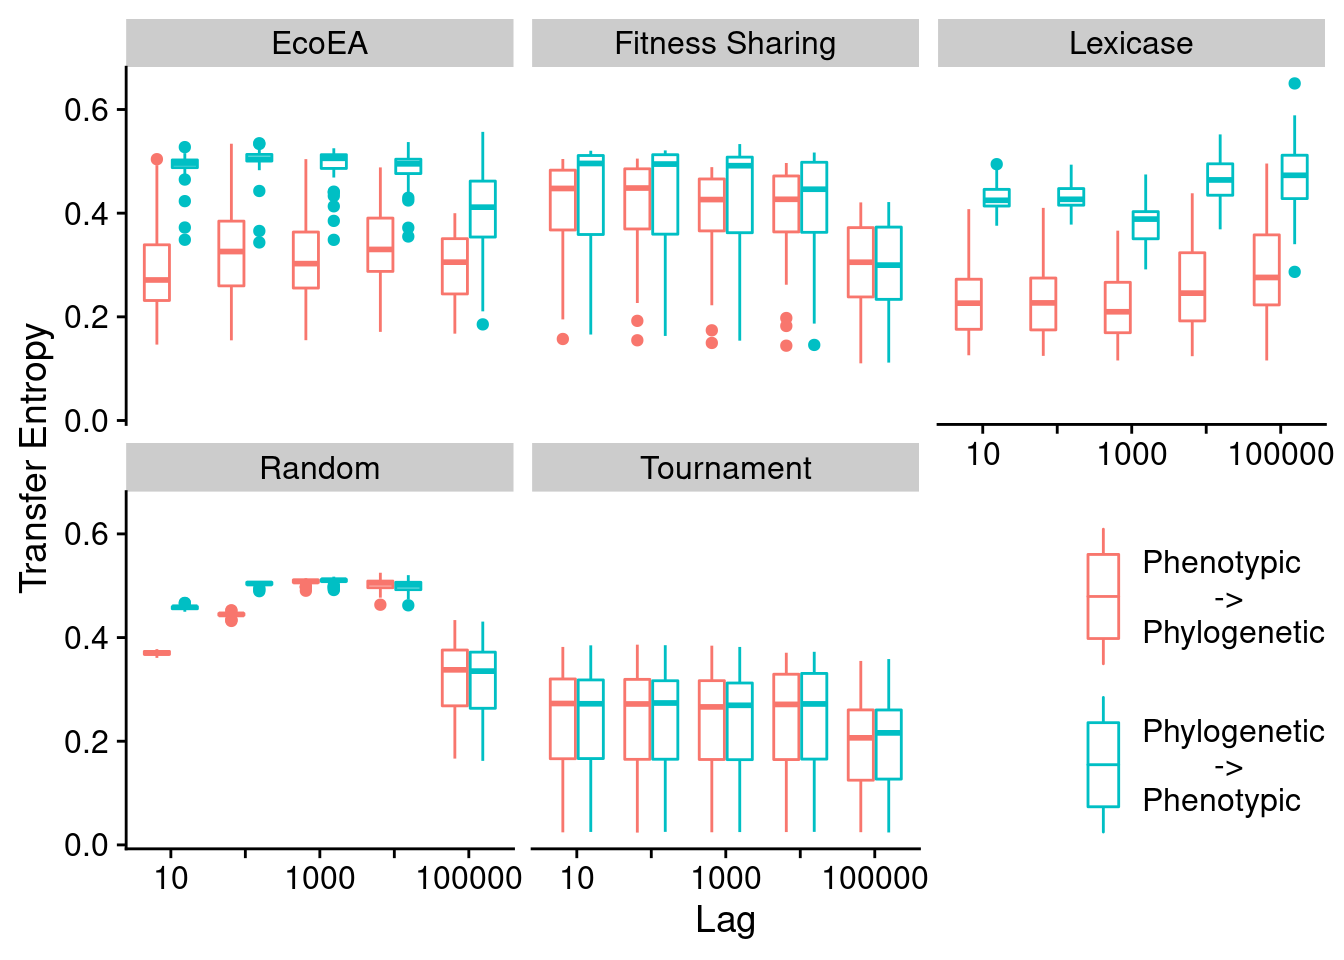
\includegraphics{phylodiversity-in-EC-supplement_files/figure-latex/information_theory_pheno_phylo_mpd_shannon-1.pdf}

\hypertarget{mean-evolutionary-distinctiveness-and-phenotypic-richness}{%
\subsubsection{Mean evolutionary distinctiveness and phenotypic richness}\label{mean-evolutionary-distinctiveness-and-phenotypic-richness}}

\begin{Shaded}
\begin{Highlighting}[]
\NormalTok{res <-}\StringTok{ }\NormalTok{data }\OperatorTok\StringTok{ }\KeywordTok{group_by}\NormalTok{(directory, selection_name) }\OperatorTok
\KeywordTok{summarise}\NormalTok{(}
  \DataTypeTok{phen_phylo_10 =}      \KeywordTok{condinformation}\NormalTok{(}
                          \KeywordTok{discretize}\NormalTok{(phen_num_taxa), }
                          \KeywordTok{discretize}\NormalTok{(}\KeywordTok{lag}\NormalTok{(mean_phenotype_evolutionary_distinctiveness, }\DecValTok{1}\NormalTok{)), }
                          \KeywordTok{discretize}\NormalTok{(}\KeywordTok{lag}\NormalTok{(phen_num_taxa, }\DecValTok{1}\NormalTok{))),}
  \DataTypeTok{phen_phylo_100 =}     \KeywordTok{condinformation}\NormalTok{(}
                          \KeywordTok{discretize}\NormalTok{(phen_num_taxa),}
                          \KeywordTok{discretize}\NormalTok{(}\KeywordTok{lag}\NormalTok{(mean_phenotype_evolutionary_distinctiveness, }\DecValTok{10}\NormalTok{)),}
                          \KeywordTok{discretize}\NormalTok{(}\KeywordTok{lag}\NormalTok{(phen_num_taxa, }\DecValTok{10}\NormalTok{))),}
  \DataTypeTok{pheno_phylo_1000 =}   \KeywordTok{condinformation}\NormalTok{(}
                          \KeywordTok{discretize}\NormalTok{(phen_num_taxa),}
                          \KeywordTok{discretize}\NormalTok{(}\KeywordTok{lag}\NormalTok{(mean_phenotype_evolutionary_distinctiveness, }\DecValTok{100}\NormalTok{)),}
                          \KeywordTok{discretize}\NormalTok{(}\KeywordTok{lag}\NormalTok{(phen_num_taxa, }\DecValTok{100}\NormalTok{))),}
  \DataTypeTok{pheno_phylo_10000 =}  \KeywordTok{condinformation}\NormalTok{(}
                          \KeywordTok{discretize}\NormalTok{(phen_num_taxa),}
                          \KeywordTok{discretize}\NormalTok{(}\KeywordTok{lag}\NormalTok{(mean_phenotype_evolutionary_distinctiveness, }\DecValTok{1000}\NormalTok{)),}
                          \KeywordTok{discretize}\NormalTok{(}\KeywordTok{lag}\NormalTok{(phen_num_taxa, }\DecValTok{1000}\NormalTok{))),}
  \DataTypeTok{pheno_phylo_100000 =} \KeywordTok{condinformation}\NormalTok{(}
                          \KeywordTok{discretize}\NormalTok{(phen_num_taxa),}
                          \KeywordTok{discretize}\NormalTok{(}\KeywordTok{lag}\NormalTok{(mean_phenotype_evolutionary_distinctiveness, }\DecValTok{10000}\NormalTok{)),}
                          \KeywordTok{discretize}\NormalTok{(}\KeywordTok{lag}\NormalTok{(phen_num_taxa, }\DecValTok{10000}\NormalTok{))),}
  
  \DataTypeTok{phylo_pheno_10 =}     \KeywordTok{condinformation}\NormalTok{(}
                          \KeywordTok{discretize}\NormalTok{(mean_phenotype_evolutionary_distinctiveness),}
                          \KeywordTok{discretize}\NormalTok{(}\KeywordTok{lag}\NormalTok{(phen_num_taxa, }\DecValTok{1}\NormalTok{)),}
                          \KeywordTok{discretize}\NormalTok{(}\KeywordTok{lag}\NormalTok{(mean_phenotype_evolutionary_distinctiveness, }\DecValTok{1}\NormalTok{))),}
  \DataTypeTok{phylo_pheno_100 =}    \KeywordTok{condinformation}\NormalTok{(}
                          \KeywordTok{discretize}\NormalTok{(mean_phenotype_evolutionary_distinctiveness),}
                          \KeywordTok{discretize}\NormalTok{(}\KeywordTok{lag}\NormalTok{(phen_num_taxa, }\DecValTok{10}\NormalTok{)),}
                          \KeywordTok{discretize}\NormalTok{(}\KeywordTok{lag}\NormalTok{(mean_phenotype_evolutionary_distinctiveness, }\DecValTok{10}\NormalTok{))),}
  \DataTypeTok{phylo_pheno_1000 =}   \KeywordTok{condinformation}\NormalTok{(}
                          \KeywordTok{discretize}\NormalTok{(mean_phenotype_evolutionary_distinctiveness),}
                          \KeywordTok{discretize}\NormalTok{(}\KeywordTok{lag}\NormalTok{(phen_num_taxa, }\DecValTok{100}\NormalTok{)),}
                          \KeywordTok{discretize}\NormalTok{(}\KeywordTok{lag}\NormalTok{(mean_phenotype_evolutionary_distinctiveness, }\DecValTok{100}\NormalTok{))),}
  \DataTypeTok{phylo_pheno_10000 =}  \KeywordTok{condinformation}\NormalTok{(}
                          \KeywordTok{discretize}\NormalTok{(mean_phenotype_evolutionary_distinctiveness),}
                          \KeywordTok{discretize}\NormalTok{(}\KeywordTok{lag}\NormalTok{(phen_num_taxa, }\DecValTok{1000}\NormalTok{)),}
                          \KeywordTok{discretize}\NormalTok{(}\KeywordTok{lag}\NormalTok{(mean_phenotype_evolutionary_distinctiveness, }\DecValTok{1000}\NormalTok{))),}
  \DataTypeTok{phylo_pheno_100000 =} \KeywordTok{condinformation}\NormalTok{(}
                          \KeywordTok{discretize}\NormalTok{(mean_phenotype_evolutionary_distinctiveness),}
                          \KeywordTok{discretize}\NormalTok{(}\KeywordTok{lag}\NormalTok{(phen_num_taxa, }\DecValTok{10000}\NormalTok{)),}
                          \KeywordTok{discretize}\NormalTok{(}\KeywordTok{lag}\NormalTok{(mean_phenotype_evolutionary_distinctiveness, }\DecValTok{10000}\NormalTok{)))}
\NormalTok{)}

\CommentTok{# Turn Transfer Entropy columns into rows}
\NormalTok{res <-}\StringTok{ }\NormalTok{res }\OperatorTok\StringTok{ }\KeywordTok{pivot_longer}\NormalTok{(}\DataTypeTok{cols=}\KeywordTok{contains}\NormalTok{(}\StringTok{"phylo"}\NormalTok{))}
\CommentTok{# Pull lag into a column}
\NormalTok{res}\OperatorTok{$}\NormalTok{offset <-}\StringTok{ }\KeywordTok{str_extract}\NormalTok{(res}\OperatorTok{$}\NormalTok{name, }\StringTok{"[:digit:]*$"}\NormalTok{)}
\CommentTok{# Make column indicating direction of transfer entropy}
\NormalTok{res}\OperatorTok{$}\NormalTok{Type <-}\StringTok{ }\KeywordTok{case_when}\NormalTok{(}\KeywordTok{str_detect}\NormalTok{(res}\OperatorTok{$}\NormalTok{name, }\StringTok{"phylo_pheno"}\NormalTok{) }\OperatorTok{~}\StringTok{ "}\CharTok{\textbackslash{}n}\StringTok{Phenotypic}\CharTok{\textbackslash{}n\textbackslash{}t}\StringTok{->}\CharTok{\textbackslash{}n}\StringTok{Phylogenetic}\CharTok{\textbackslash{}n}\StringTok{"}\NormalTok{, }\OtherTok{TRUE} \OperatorTok{~}\StringTok{ "}\CharTok{\textbackslash{}n}\StringTok{Phylogenetic}\CharTok{\textbackslash{}n\textbackslash{}t}\StringTok{->}\CharTok{\textbackslash{}n}\StringTok{Phenotypic}\CharTok{\textbackslash{}n}\StringTok{"}\NormalTok{)}

\KeywordTok{ggplot}\NormalTok{(}
\NormalTok{  res, }
  \KeywordTok{aes}\NormalTok{(}
    \DataTypeTok{x=}\KeywordTok{as.factor}\NormalTok{(offset), }
    \DataTypeTok{y=}\NormalTok{value, }
    \DataTypeTok{color=}\NormalTok{Type}
\NormalTok{    )}
\NormalTok{  ) }\OperatorTok{+}\StringTok{ }
\StringTok{  }\KeywordTok{geom_boxplot}\NormalTok{() }\OperatorTok{+}\StringTok{ }
\StringTok{  }\KeywordTok{facet_wrap}\NormalTok{(}\OperatorTok{~}\NormalTok{selection_name) }\OperatorTok{+}\StringTok{ }
\StringTok{  }\KeywordTok{scale_x_discrete}\NormalTok{(}\StringTok{"Lag"}\NormalTok{,}\DataTypeTok{labels=}\KeywordTok{c}\NormalTok{(}\StringTok{"10"}\NormalTok{,}\StringTok{""}\NormalTok{,}\StringTok{"1000"}\NormalTok{,}\StringTok{""}\NormalTok{,}\StringTok{"100000"}\NormalTok{)) }\OperatorTok{+}\StringTok{ }
\StringTok{  }\KeywordTok{scale_y_continuous}\NormalTok{(}\StringTok{"Transfer Entropy"}\NormalTok{) }\OperatorTok{+}\StringTok{ }
\StringTok{  }\KeywordTok{theme}\NormalTok{(}\DataTypeTok{legend.position =} \KeywordTok{c}\NormalTok{(}\DecValTok{1}\NormalTok{, }\DecValTok{0}\NormalTok{),}
        \DataTypeTok{legend.justification =} \KeywordTok{c}\NormalTok{(}\DecValTok{1}\NormalTok{, }\DecValTok{0}\NormalTok{)) }\OperatorTok{+}\StringTok{ }
\StringTok{  }\KeywordTok{scale_color_discrete}\NormalTok{(}\StringTok{""}\NormalTok{)}
\end{Highlighting}
\end{Shaded}

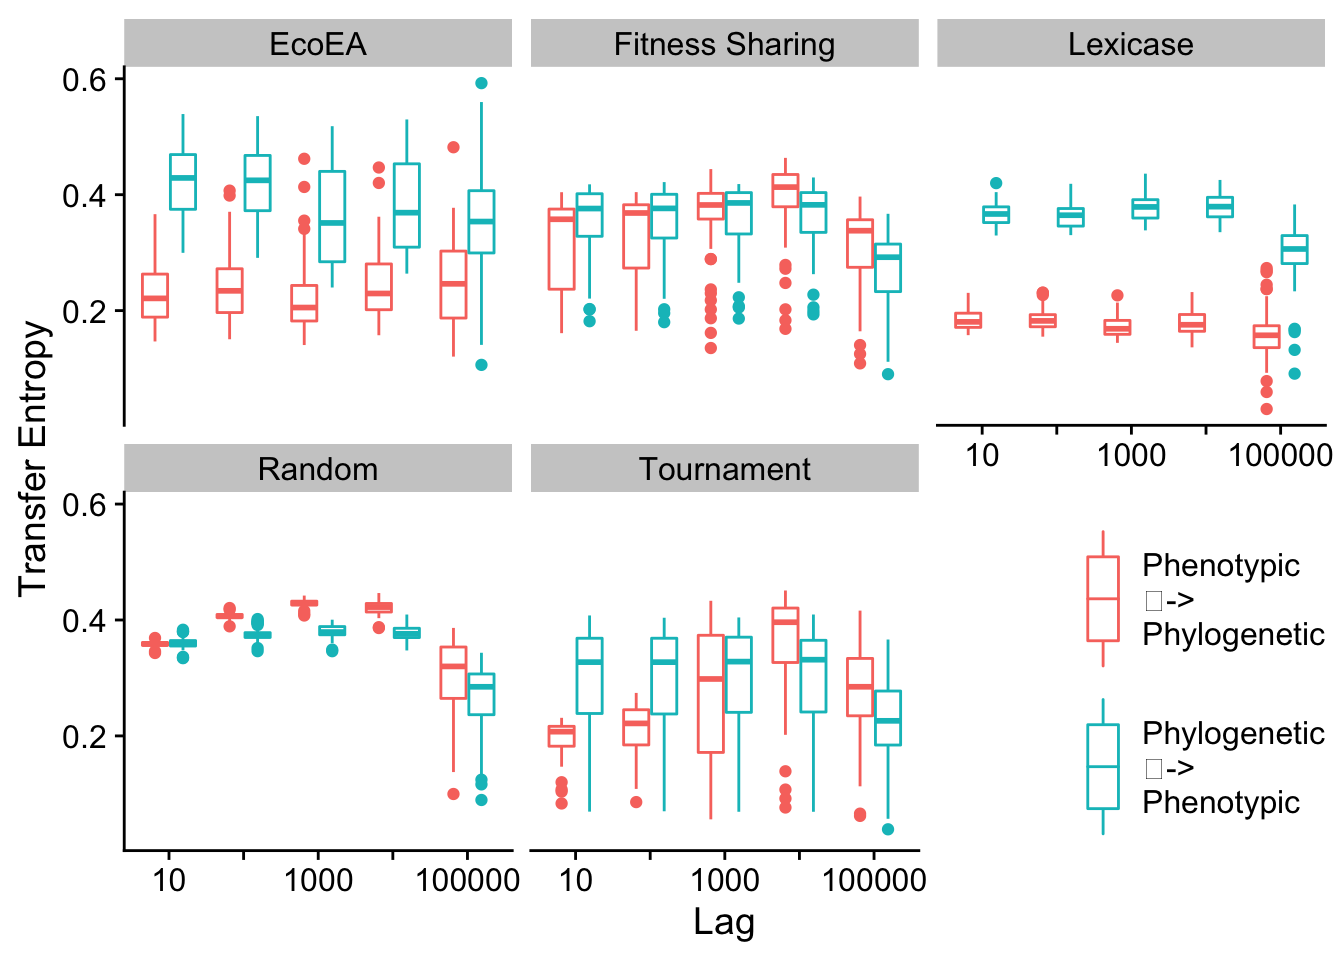
\includegraphics{phylodiversity-in-EC-supplement_files/figure-latex/information_theory_pheno_phylo_med-1.pdf}

\hypertarget{mean-evolutionary-distinctiveness-and-shannon-diversity}{%
\subsubsection{Mean evolutionary distinctiveness and shannon diversity}\label{mean-evolutionary-distinctiveness-and-shannon-diversity}}

\begin{Shaded}
\begin{Highlighting}[]
\NormalTok{res <-}\StringTok{ }\NormalTok{data }\OperatorTok\StringTok{ }\KeywordTok{group_by}\NormalTok{(directory, selection_name) }\OperatorTok
\KeywordTok{summarise}\NormalTok{(}
  \DataTypeTok{phen_phylo_10 =}      \KeywordTok{condinformation}\NormalTok{(}
                          \KeywordTok{discretize}\NormalTok{(phen_diversity), }
                          \KeywordTok{discretize}\NormalTok{(}\KeywordTok{lag}\NormalTok{(mean_phenotype_evolutionary_distinctiveness, }\DecValTok{1}\NormalTok{)), }
                          \KeywordTok{discretize}\NormalTok{(}\KeywordTok{lag}\NormalTok{(phen_diversity, }\DecValTok{1}\NormalTok{))),}
  \DataTypeTok{phen_phylo_100 =}     \KeywordTok{condinformation}\NormalTok{(}
                          \KeywordTok{discretize}\NormalTok{(phen_diversity),}
                          \KeywordTok{discretize}\NormalTok{(}\KeywordTok{lag}\NormalTok{(mean_phenotype_evolutionary_distinctiveness, }\DecValTok{10}\NormalTok{)),}
                          \KeywordTok{discretize}\NormalTok{(}\KeywordTok{lag}\NormalTok{(phen_diversity, }\DecValTok{10}\NormalTok{))),}
  \DataTypeTok{pheno_phylo_1000 =}   \KeywordTok{condinformation}\NormalTok{(}
                          \KeywordTok{discretize}\NormalTok{(phen_diversity),}
                          \KeywordTok{discretize}\NormalTok{(}\KeywordTok{lag}\NormalTok{(mean_phenotype_evolutionary_distinctiveness, }\DecValTok{100}\NormalTok{)),}
                          \KeywordTok{discretize}\NormalTok{(}\KeywordTok{lag}\NormalTok{(phen_diversity, }\DecValTok{100}\NormalTok{))),}
  \DataTypeTok{pheno_phylo_10000 =}  \KeywordTok{condinformation}\NormalTok{(}
                          \KeywordTok{discretize}\NormalTok{(phen_diversity),}
                          \KeywordTok{discretize}\NormalTok{(}\KeywordTok{lag}\NormalTok{(mean_phenotype_evolutionary_distinctiveness, }\DecValTok{1000}\NormalTok{)),}
                          \KeywordTok{discretize}\NormalTok{(}\KeywordTok{lag}\NormalTok{(phen_diversity, }\DecValTok{1000}\NormalTok{))),}
  \DataTypeTok{pheno_phylo_100000 =} \KeywordTok{condinformation}\NormalTok{(}
                          \KeywordTok{discretize}\NormalTok{(phen_diversity),}
                          \KeywordTok{discretize}\NormalTok{(}\KeywordTok{lag}\NormalTok{(mean_phenotype_evolutionary_distinctiveness, }\DecValTok{10000}\NormalTok{)),}
                          \KeywordTok{discretize}\NormalTok{(}\KeywordTok{lag}\NormalTok{(phen_diversity, }\DecValTok{10000}\NormalTok{))),}
  
  \DataTypeTok{phylo_pheno_10 =}     \KeywordTok{condinformation}\NormalTok{(}
                          \KeywordTok{discretize}\NormalTok{(mean_phenotype_evolutionary_distinctiveness),}
                          \KeywordTok{discretize}\NormalTok{(}\KeywordTok{lag}\NormalTok{(phen_diversity, }\DecValTok{1}\NormalTok{)),}
                          \KeywordTok{discretize}\NormalTok{(}\KeywordTok{lag}\NormalTok{(mean_phenotype_evolutionary_distinctiveness, }\DecValTok{1}\NormalTok{))),}
  \DataTypeTok{phylo_pheno_100 =}    \KeywordTok{condinformation}\NormalTok{(}
                          \KeywordTok{discretize}\NormalTok{(mean_phenotype_evolutionary_distinctiveness),}
                          \KeywordTok{discretize}\NormalTok{(}\KeywordTok{lag}\NormalTok{(phen_diversity, }\DecValTok{10}\NormalTok{)),}
                          \KeywordTok{discretize}\NormalTok{(}\KeywordTok{lag}\NormalTok{(mean_phenotype_evolutionary_distinctiveness, }\DecValTok{10}\NormalTok{))),}
  \DataTypeTok{phylo_pheno_1000 =}   \KeywordTok{condinformation}\NormalTok{(}
                          \KeywordTok{discretize}\NormalTok{(mean_phenotype_evolutionary_distinctiveness),}
                          \KeywordTok{discretize}\NormalTok{(}\KeywordTok{lag}\NormalTok{(phen_diversity, }\DecValTok{100}\NormalTok{)),}
                          \KeywordTok{discretize}\NormalTok{(}\KeywordTok{lag}\NormalTok{(mean_phenotype_evolutionary_distinctiveness, }\DecValTok{100}\NormalTok{))),}
  \DataTypeTok{phylo_pheno_10000 =}  \KeywordTok{condinformation}\NormalTok{(}
                          \KeywordTok{discretize}\NormalTok{(mean_phenotype_evolutionary_distinctiveness),}
                          \KeywordTok{discretize}\NormalTok{(}\KeywordTok{lag}\NormalTok{(phen_diversity, }\DecValTok{1000}\NormalTok{)),}
                          \KeywordTok{discretize}\NormalTok{(}\KeywordTok{lag}\NormalTok{(mean_phenotype_evolutionary_distinctiveness, }\DecValTok{1000}\NormalTok{))),}
  \DataTypeTok{phylo_pheno_100000 =} \KeywordTok{condinformation}\NormalTok{(}
                          \KeywordTok{discretize}\NormalTok{(mean_phenotype_evolutionary_distinctiveness),}
                          \KeywordTok{discretize}\NormalTok{(}\KeywordTok{lag}\NormalTok{(phen_diversity, }\DecValTok{10000}\NormalTok{)),}
                          \KeywordTok{discretize}\NormalTok{(}\KeywordTok{lag}\NormalTok{(mean_phenotype_evolutionary_distinctiveness, }\DecValTok{10000}\NormalTok{)))}
\NormalTok{)}

\CommentTok{# Turn Transfer Entropy columns into rows}
\NormalTok{res <-}\StringTok{ }\NormalTok{res }\OperatorTok\StringTok{ }\KeywordTok{pivot_longer}\NormalTok{(}\DataTypeTok{cols=}\KeywordTok{contains}\NormalTok{(}\StringTok{"phylo"}\NormalTok{))}
\CommentTok{# Pull lag into a column}
\NormalTok{res}\OperatorTok{$}\NormalTok{offset <-}\StringTok{ }\KeywordTok{str_extract}\NormalTok{(res}\OperatorTok{$}\NormalTok{name, }\StringTok{"[:digit:]*$"}\NormalTok{)}
\CommentTok{# Make column indicating direction of transfer entropy}
\NormalTok{res}\OperatorTok{$}\NormalTok{Type <-}\StringTok{ }\KeywordTok{case_when}\NormalTok{(}\KeywordTok{str_detect}\NormalTok{(res}\OperatorTok{$}\NormalTok{name, }\StringTok{"phylo_pheno"}\NormalTok{) }\OperatorTok{~}\StringTok{ "}\CharTok{\textbackslash{}n}\StringTok{Phenotypic}\CharTok{\textbackslash{}n\textbackslash{}t}\StringTok{->}\CharTok{\textbackslash{}n}\StringTok{Phylogenetic}\CharTok{\textbackslash{}n}\StringTok{"}\NormalTok{, }\OtherTok{TRUE} \OperatorTok{~}\StringTok{ "}\CharTok{\textbackslash{}n}\StringTok{Phylogenetic}\CharTok{\textbackslash{}n\textbackslash{}t}\StringTok{->}\CharTok{\textbackslash{}n}\StringTok{Phenotypic}\CharTok{\textbackslash{}n}\StringTok{"}\NormalTok{)}

\KeywordTok{ggplot}\NormalTok{(}
\NormalTok{  res, }
  \KeywordTok{aes}\NormalTok{(}
    \DataTypeTok{x=}\KeywordTok{as.factor}\NormalTok{(offset), }
    \DataTypeTok{y=}\NormalTok{value, }
    \DataTypeTok{color=}\NormalTok{Type}
\NormalTok{    )}
\NormalTok{  ) }\OperatorTok{+}\StringTok{ }
\StringTok{  }\KeywordTok{geom_boxplot}\NormalTok{() }\OperatorTok{+}\StringTok{ }
\StringTok{  }\KeywordTok{facet_wrap}\NormalTok{(}\OperatorTok{~}\NormalTok{selection_name) }\OperatorTok{+}\StringTok{ }
\StringTok{  }\KeywordTok{scale_x_discrete}\NormalTok{(}\StringTok{"Lag"}\NormalTok{,}\DataTypeTok{labels=}\KeywordTok{c}\NormalTok{(}\StringTok{"10"}\NormalTok{,}\StringTok{""}\NormalTok{,}\StringTok{"1000"}\NormalTok{,}\StringTok{""}\NormalTok{,}\StringTok{"100000"}\NormalTok{)) }\OperatorTok{+}\StringTok{ }
\StringTok{  }\KeywordTok{scale_y_continuous}\NormalTok{(}\StringTok{"Transfer Entropy"}\NormalTok{) }\OperatorTok{+}\StringTok{ }
\StringTok{  }\KeywordTok{theme}\NormalTok{(}\DataTypeTok{legend.position =} \KeywordTok{c}\NormalTok{(}\DecValTok{1}\NormalTok{, }\DecValTok{0}\NormalTok{),}
        \DataTypeTok{legend.justification =} \KeywordTok{c}\NormalTok{(}\DecValTok{1}\NormalTok{, }\DecValTok{0}\NormalTok{)) }\OperatorTok{+}\StringTok{ }
\StringTok{  }\KeywordTok{scale_color_discrete}\NormalTok{(}\StringTok{""}\NormalTok{)}
\end{Highlighting}
\end{Shaded}

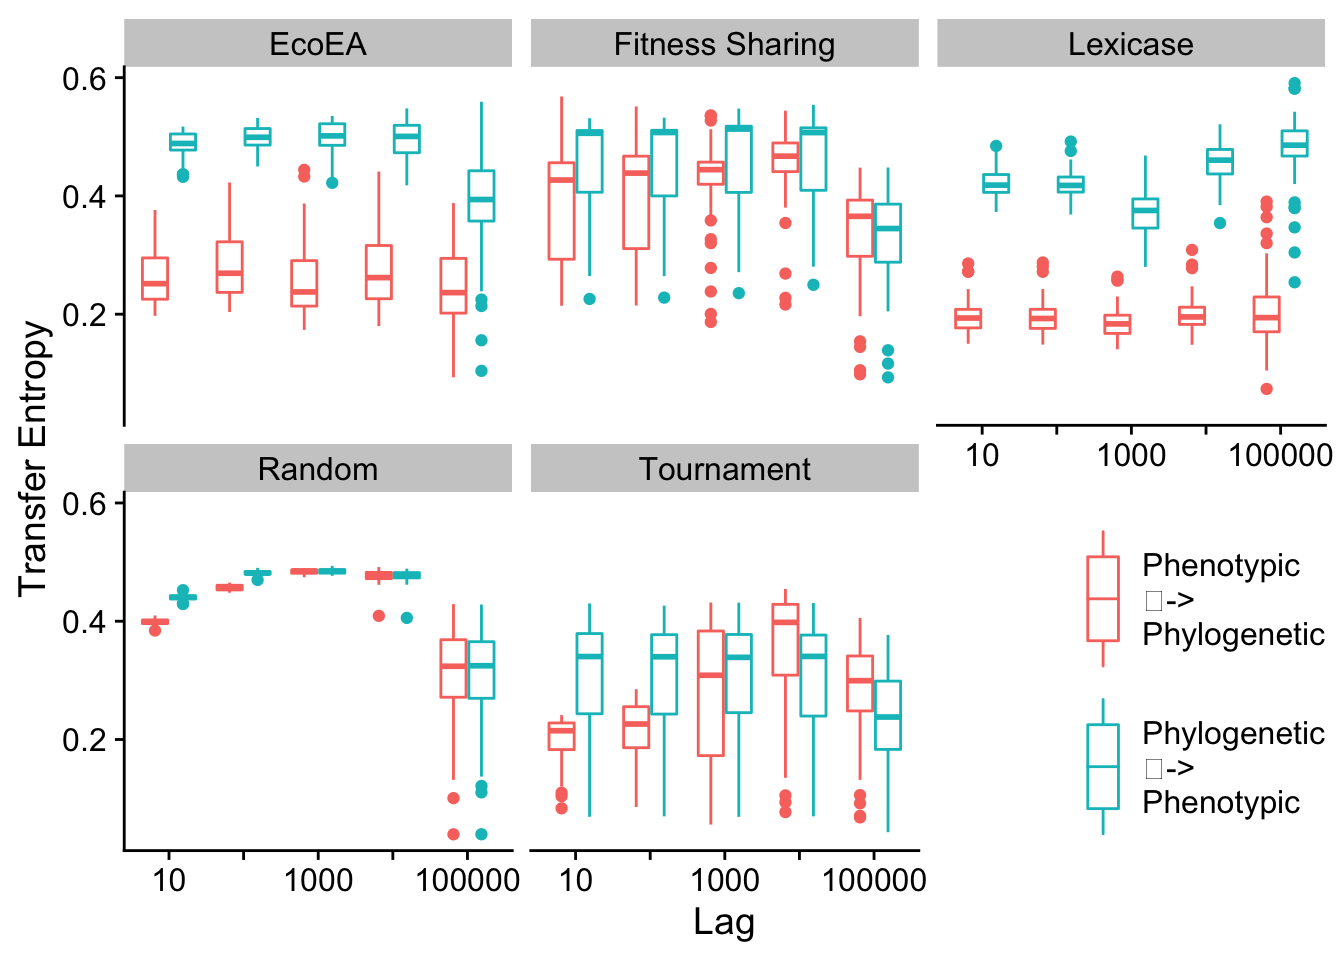
\includegraphics{phylodiversity-in-EC-supplement_files/figure-latex/information_theory_pheno_phylo_med_shannon-1.pdf}

\hypertarget{other-fitness-landscapes}{%
\chapter{Other fitness landscapes}\label{other-fitness-landscapes}}

\hypertarget{setup-1}{%
\section{Setup}\label{setup-1}}

\begin{Shaded}
\begin{Highlighting}[]
\KeywordTok{library}\NormalTok{(ggplot2)}
\KeywordTok{library}\NormalTok{(tidyverse)}
\KeywordTok{library}\NormalTok{(knitr)}
\KeywordTok{library}\NormalTok{(cowplot)}
\KeywordTok{library}\NormalTok{(viridis)}
\KeywordTok{library}\NormalTok{(RColorBrewer)}
\KeywordTok{library}\NormalTok{(rstatix)}
\KeywordTok{library}\NormalTok{(ggsignif)}
\KeywordTok{library}\NormalTok{(Hmisc)}
\KeywordTok{library}\NormalTok{(kableExtra)}
\KeywordTok{source}\NormalTok{(}\StringTok{"https://gist.githubusercontent.com/benmarwick/2a1bb0133ff568cbe28d/raw/fb53bd97121f7f9ce947837ef1a4c65a73bffb3f/geom_flat_violin.R"}\NormalTok{)}
\KeywordTok{library}\NormalTok{(readr)}
\KeywordTok{library}\NormalTok{(stringr)}
\KeywordTok{library}\NormalTok{(ggpubr)}
\KeywordTok{library}\NormalTok{(infotheo)}
\KeywordTok{library}\NormalTok{(osfr)}
\end{Highlighting}
\end{Shaded}

These analyses were conducted in the following computing environment:

\begin{Shaded}
\begin{Highlighting}[]
\KeywordTok{print}\NormalTok{(version)}
\end{Highlighting}
\end{Shaded}

\begin{verbatim}
##                _                           
## platform       x86_64-pc-linux-gnu         
## arch           x86_64                      
## os             linux-gnu                   
## system         x86_64, linux-gnu           
## status                                     
## major          4                           
## minor          0.4                         
## year           2021                        
## month          02                          
## day            15                          
## svn rev        80002                       
## language       R                           
## version.string R version 4.0.4 (2021-02-15)
## nickname       Lost Library Book
\end{verbatim}

\begin{Shaded}
\begin{Highlighting}[]
\CommentTok{# Labeler for stats annotations}
\NormalTok{p_label <-}\StringTok{ }\ControlFlowTok{function}\NormalTok{(p_value) \{}
\NormalTok{  threshold =}\StringTok{ }\FloatTok{0.0001}
  \ControlFlowTok{if}\NormalTok{ (p_value }\OperatorTok{<}\StringTok{ }\NormalTok{threshold) \{}
    \KeywordTok{return}\NormalTok{(}\KeywordTok{paste0}\NormalTok{(}\StringTok{"p < "}\NormalTok{, threshold))}
\NormalTok{  \} }\ControlFlowTok{else}\NormalTok{ \{}
    \KeywordTok{return}\NormalTok{(}\KeywordTok{paste0}\NormalTok{(}\StringTok{"p = "}\NormalTok{, p_value))}
\NormalTok{  \}}
\NormalTok{\}}

\CommentTok{# Significance threshold}
\NormalTok{alpha <-}\StringTok{ }\FloatTok{0.05}

\CommentTok{####### misc #######}
\CommentTok{# Configure our default graphing theme}
\KeywordTok{theme_set}\NormalTok{(}\KeywordTok{theme_cowplot}\NormalTok{())}
\end{Highlighting}
\end{Shaded}

\begin{Shaded}
\begin{Highlighting}[]
\KeywordTok{osf_retrieve_file}\NormalTok{(}\StringTok{"p79hx"}\NormalTok{) }\OperatorTok\StringTok{ }\KeywordTok{osf_download}\NormalTok{(}\DataTypeTok{conflicts =} \StringTok{"skip"}\NormalTok{)  }\CommentTok{# Download data from osf}
\end{Highlighting}
\end{Shaded}

\begin{verbatim}
## # A tibble: 1 x 4
##   name                   id                local_path               meta        
##   <chr>                  <chr>             <chr>                    <list>      
## 1 complex_fitness_lands~ 612fe4d84e5ee501~ ./complex_fitness_lands~ <named list~
\end{verbatim}

\begin{Shaded}
\begin{Highlighting}[]
\NormalTok{data_loc <-}\StringTok{ "complex_fitness_landscapes.csv"}

\NormalTok{data <-}\StringTok{ }\KeywordTok{read_csv}\NormalTok{(data_loc, }\DataTypeTok{na=}\KeywordTok{c}\NormalTok{(}\StringTok{"NONE"}\NormalTok{, }\StringTok{"NA"}\NormalTok{, }\StringTok{""}\NormalTok{))}

\NormalTok{data <-}\StringTok{ }\NormalTok{data }\OperatorTok\StringTok{ }
\StringTok{  }\KeywordTok{filter}\NormalTok{(N}\OperatorTok{==}\DecValTok{20}\NormalTok{, generation }\OperatorTok\DecValTok{10} \OperatorTok{==}\StringTok{ }\DecValTok{0}\NormalTok{) }\OperatorTok
\StringTok{  }\KeywordTok{mutate}\NormalTok{(}
  \DataTypeTok{selection_name =} \KeywordTok{as.factor}\NormalTok{(}\KeywordTok{case_when}\NormalTok{(}
\NormalTok{    SELECTION }\OperatorTok{==}\StringTok{ }\DecValTok{0} \OperatorTok{~}\StringTok{ "Tournament"}\NormalTok{,}
\NormalTok{    SELECTION }\OperatorTok{==}\StringTok{ }\DecValTok{1} \OperatorTok{~}\StringTok{ "Fitness sharing"}\NormalTok{,}
\NormalTok{    SELECTION }\OperatorTok{==}\StringTok{ }\DecValTok{2} \OperatorTok{~}\StringTok{ "Lexicase"}\NormalTok{,}
\NormalTok{    SELECTION }\OperatorTok{==}\StringTok{ }\DecValTok{3} \OperatorTok{~}\StringTok{ "Eco-EA"}\NormalTok{,}
\NormalTok{    SELECTION }\OperatorTok{==}\StringTok{ }\DecValTok{4} \OperatorTok{~}\StringTok{ "Random"}\NormalTok{,}
\NormalTok{  )), }
  \DataTypeTok{problem_name =} \KeywordTok{as.factor}\NormalTok{(}\KeywordTok{case_when}\NormalTok{(}
\NormalTok{    PROBLEM }\OperatorTok{==}\StringTok{ }\DecValTok{0} \OperatorTok{~}\StringTok{ "NK Landscape"}\NormalTok{,}
\NormalTok{    PROBLEM }\OperatorTok{==}\StringTok{ }\DecValTok{1} \OperatorTok{~}\StringTok{ "Count Odds"}\NormalTok{,}
\NormalTok{    PROBLEM }\OperatorTok{==}\StringTok{ }\DecValTok{2} \OperatorTok{~}\StringTok{ "Real-valued optimization"}\NormalTok{,}
\NormalTok{    PROBLEM }\OperatorTok{==}\StringTok{ }\DecValTok{3} \OperatorTok{~}\StringTok{ "Sorting network"}\NormalTok{,}
\NormalTok{    PROBLEM }\OperatorTok{==}\StringTok{ }\DecValTok{4} \OperatorTok{~}\StringTok{ "Logic-9"}    
\NormalTok{  ))}
\NormalTok{)}

\NormalTok{final_data <-}\StringTok{ }\KeywordTok{filter}\NormalTok{(data, generation}\OperatorTok{==}\KeywordTok{max}\NormalTok{(data}\OperatorTok{$}\NormalTok{generation))}
\end{Highlighting}
\end{Shaded}

\hypertarget{performance-1}{%
\section{Performance}\label{performance-1}}

\hypertarget{over-time-3}{%
\subsection{Over time}\label{over-time-3}}

\begin{Shaded}
\begin{Highlighting}[]
\KeywordTok{ggplot}\NormalTok{(}
\NormalTok{    data,}
    \KeywordTok{aes}\NormalTok{(}
      \DataTypeTok{x=}\NormalTok{generation,}
      \DataTypeTok{y=}\NormalTok{max_performance,}
      \DataTypeTok{color=}\NormalTok{selection_name,}
      \DataTypeTok{fill=}\NormalTok{selection_name}
\NormalTok{    )}
\NormalTok{  ) }\OperatorTok{+}
\StringTok{  }\KeywordTok{stat_summary}\NormalTok{(}\DataTypeTok{geom=}\StringTok{"line"}\NormalTok{, }\DataTypeTok{fun=}\NormalTok{mean) }\OperatorTok{+}
\StringTok{  }\KeywordTok{stat_summary}\NormalTok{(}
    \DataTypeTok{geom=}\StringTok{"ribbon"}\NormalTok{,}
    \DataTypeTok{fun.data=}\StringTok{"mean_cl_boot"}\NormalTok{,}
    \DataTypeTok{fun.args=}\KeywordTok{list}\NormalTok{(}\DataTypeTok{conf.int=}\FloatTok{0.95}\NormalTok{),}
    \DataTypeTok{alpha=}\FloatTok{0.2}\NormalTok{,}
    \DataTypeTok{linetype=}\DecValTok{0}
\NormalTok{  ) }\OperatorTok{+}
\StringTok{  }\KeywordTok{scale_y_continuous}\NormalTok{(}
    \DataTypeTok{name=}\StringTok{"Average trait performance"}
\NormalTok{  ) }\OperatorTok{+}
\StringTok{  }\KeywordTok{scale_x_continuous}\NormalTok{(}
    \DataTypeTok{name=}\StringTok{"Generation"}
\NormalTok{  ) }\OperatorTok{+}
\StringTok{  }\KeywordTok{scale_color_discrete}\NormalTok{(}\StringTok{"Selection"}\NormalTok{) }\OperatorTok{+}\StringTok{ }
\StringTok{  }\KeywordTok{scale_fill_discrete}\NormalTok{(}\StringTok{"Selection"}\NormalTok{) }\OperatorTok{+}
\StringTok{  }\KeywordTok{facet_wrap}\NormalTok{(}\OperatorTok{~}\NormalTok{problem_name, }\DataTypeTok{scales=}\StringTok{"free"}\NormalTok{)}
\end{Highlighting}
\end{Shaded}

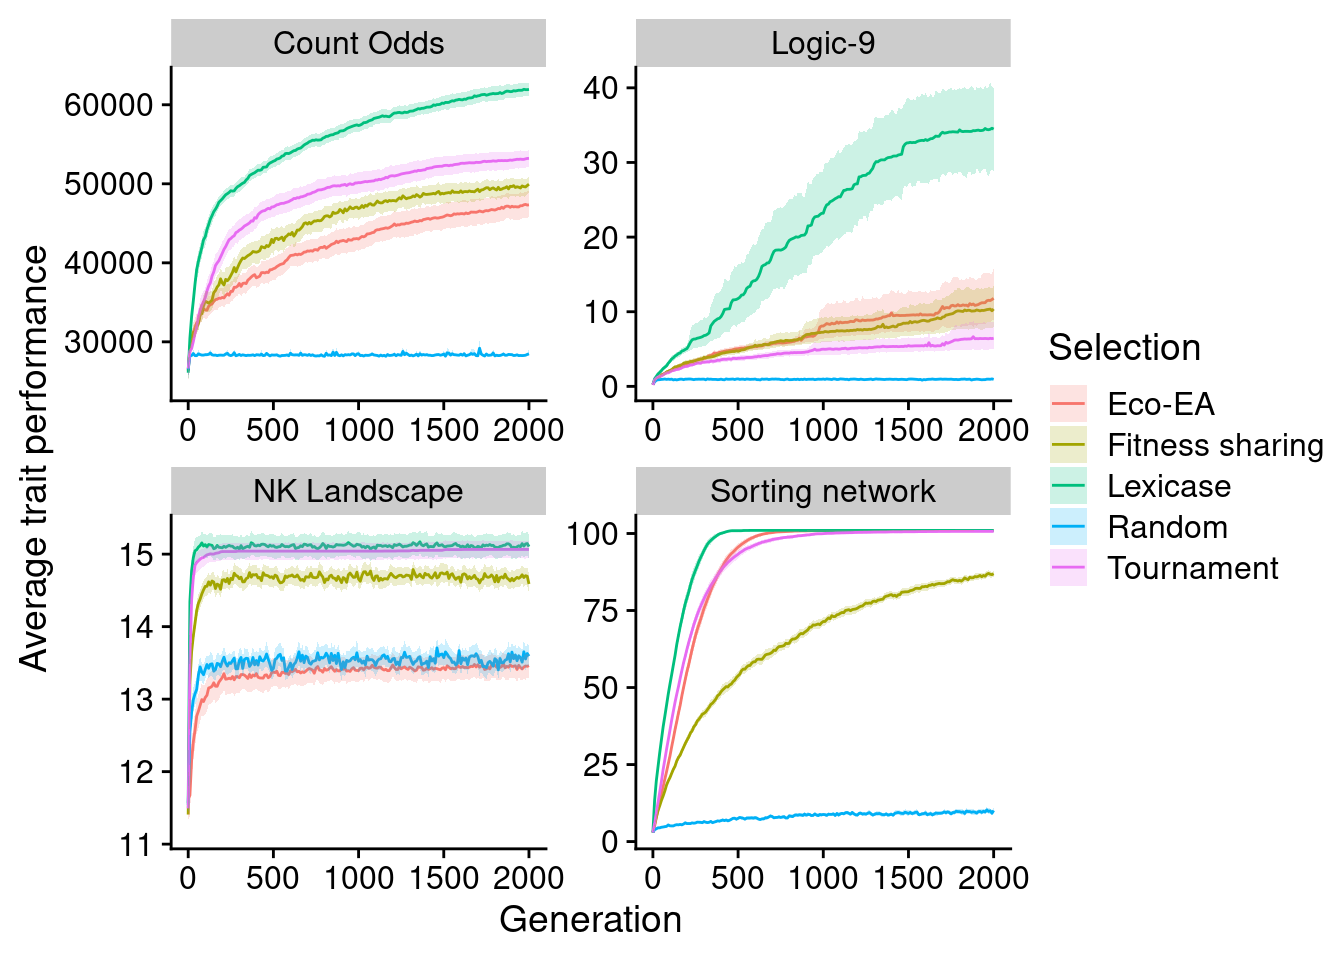
\includegraphics{phylodiversity-in-EC-supplement_files/figure-latex/complex_landscape_performance_over_time-1.pdf}

\hypertarget{final-3}{%
\subsection{Final}\label{final-3}}

\begin{Shaded}
\begin{Highlighting}[]
\CommentTok{# Compute manual labels for geom_signif}
\NormalTok{stat.test <-}\StringTok{ }\NormalTok{final_data }\OperatorTok
\StringTok{  }\KeywordTok{wilcox_test}\NormalTok{(max_performance }\OperatorTok{~}\StringTok{ }\NormalTok{selection_name) }\OperatorTok
\StringTok{  }\KeywordTok{adjust_pvalue}\NormalTok{(}\DataTypeTok{method =} \StringTok{"bonferroni"}\NormalTok{) }\OperatorTok
\StringTok{  }\KeywordTok{add_significance}\NormalTok{() }\OperatorTok
\StringTok{  }\KeywordTok{add_xy_position}\NormalTok{(}\DataTypeTok{x=}\StringTok{"selection_name"}\NormalTok{,}\DataTypeTok{step.increase=}\DecValTok{1}\NormalTok{)}
\CommentTok{#stat.test$manual_position <- stat.test$y.position * .5}
\CommentTok{#stat.test$manual_position <- c(110, 150, 170, 170, 130, 110)}
\NormalTok{stat.test}\OperatorTok{$}\NormalTok{label <-}\StringTok{ }\KeywordTok{mapply}\NormalTok{(p_label,stat.test}\OperatorTok{$}\NormalTok{p.adj)}
\end{Highlighting}
\end{Shaded}

\begin{Shaded}
\begin{Highlighting}[]
\KeywordTok{ggplot}\NormalTok{(}
\NormalTok{    final_data,}
    \KeywordTok{aes}\NormalTok{(}
      \DataTypeTok{x=}\NormalTok{selection_name,}
      \DataTypeTok{y=}\NormalTok{max_performance,}
      \DataTypeTok{fill=}\NormalTok{selection_name}
\NormalTok{    )}
\NormalTok{  ) }\OperatorTok{+}
\StringTok{  }\KeywordTok{geom_boxplot}\NormalTok{() }\OperatorTok{+}
\StringTok{  }\KeywordTok{scale_y_continuous}\NormalTok{(}
    \DataTypeTok{name=}\StringTok{"Average trait performance"}
\NormalTok{  ) }\OperatorTok{+}
\StringTok{  }\KeywordTok{scale_x_discrete}\NormalTok{(}
    \DataTypeTok{name=}\StringTok{"Selection"}
\NormalTok{  ) }\OperatorTok{+}
\StringTok{  }\KeywordTok{scale_fill_discrete}\NormalTok{(}
    \DataTypeTok{name=}\StringTok{"Selection"}
\NormalTok{  ) }\OperatorTok{+}
\StringTok{  }\KeywordTok{scale_color_discrete}\NormalTok{(}
    \DataTypeTok{name=}\StringTok{"Selection"}
\NormalTok{  ) }\OperatorTok{+}\StringTok{ }
\StringTok{  }\KeywordTok{theme}\NormalTok{(}\DataTypeTok{legend.position=}\StringTok{"none"}\NormalTok{) }\OperatorTok{+}
\StringTok{  }\KeywordTok{facet_wrap}\NormalTok{(}\OperatorTok{~}\NormalTok{problem_name, }\DataTypeTok{scales=}\StringTok{"free"}\NormalTok{)}
\end{Highlighting}
\end{Shaded}

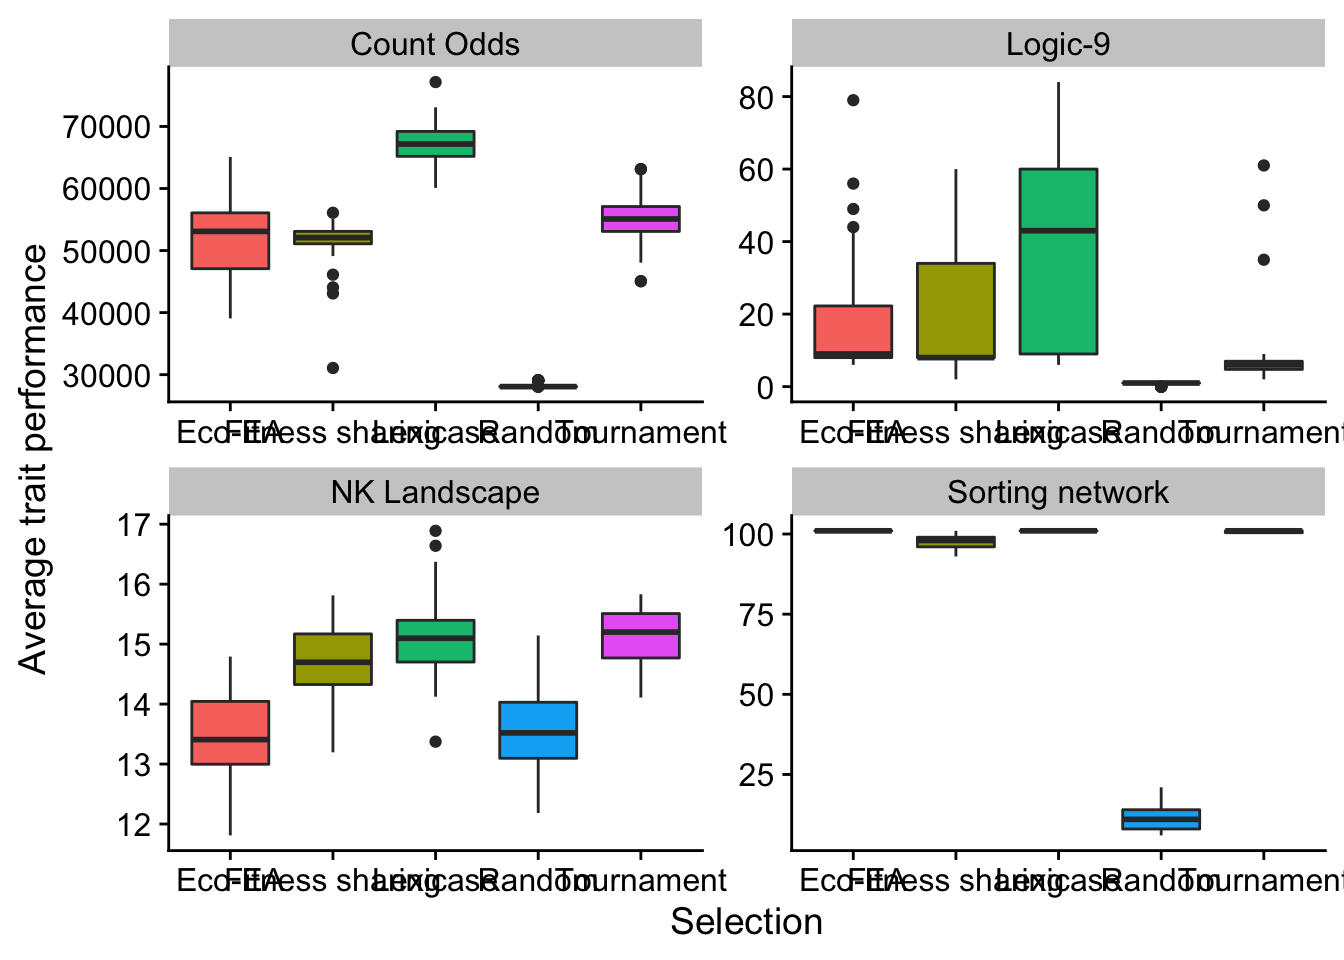
\includegraphics{phylodiversity-in-EC-supplement_files/figure-latex/complex_landscape_final_performance_plot-1.pdf}

\begin{Shaded}
\begin{Highlighting}[]
\NormalTok{stat.test }\OperatorTok
\StringTok{  }\KeywordTok{kbl}\NormalTok{() }\OperatorTok
\StringTok{  }\KeywordTok{kable_styling}\NormalTok{(}
    \DataTypeTok{bootstrap_options =} \KeywordTok{c}\NormalTok{(}
      \StringTok{"striped"}\NormalTok{,}
      \StringTok{"hover"}\NormalTok{,}
      \StringTok{"condensed"}\NormalTok{,}
      \StringTok{"responsive"}
\NormalTok{    )}
\NormalTok{  ) }\OperatorTok
\StringTok{  }\KeywordTok{scroll_box}\NormalTok{(}\DataTypeTok{width=}\StringTok{"600px"}\NormalTok{)}
\end{Highlighting}
\end{Shaded}

\begin{table}
\centering
\begin{tabular}[t]{l|l|l|r|r|r|r|r|l|r|l|r|r|l}
\hline
.y. & group1 & group2 & n1 & n2 & statistic & p & p.adj & p.adj.signif & y.position & groups & xmin & xmax & label\\
\hline
max\_performance & Eco-EA & Fitness sharing & 240 & 240 & 29310.5 & 7.37e-01 & 1.000000 & ns & 125237.4 & Eco-EA         , Fitness sharing & 1 & 2 & p = 1\\
\hline
max\_performance & Eco-EA & Lexicase & 240 & 240 & 23075.0 & 1.46e-04 & 0.001460 & ** & 178661.5 & Eco-EA  , Lexicase & 1 & 3 & p = 0.00146\\
\hline
max\_performance & Eco-EA & Random & 240 & 240 & 39696.5 & 0.00e+00 & 0.000000 & **** & 232085.6 & Eco-EA, Random & 1 & 4 & p < 1e-04\\
\hline
max\_performance & Eco-EA & Tournament & 240 & 240 & 29346.0 & 7.18e-01 & 1.000000 & ns & 285509.7 & Eco-EA    , Tournament & 1 & 5 & p = 1\\
\hline
max\_performance & Fitness sharing & Lexicase & 240 & 240 & 22328.5 & 2.01e-05 & 0.000201 & *** & 338933.8 & Fitness sharing, Lexicase & 2 & 3 & p = 0.000201\\
\hline
max\_performance & Fitness sharing & Random & 240 & 240 & 41293.0 & 0.00e+00 & 0.000000 & **** & 392358.0 & Fitness sharing, Random & 2 & 4 & p < 1e-04\\
\hline
max\_performance & Fitness sharing & Tournament & 240 & 240 & 27500.5 & 3.92e-01 & 1.000000 & ns & 445782.1 & Fitness sharing, Tournament & 2 & 5 & p = 1\\
\hline
max\_performance & Lexicase & Random & 240 & 240 & 44132.5 & 0.00e+00 & 0.000000 & **** & 499206.2 & Lexicase, Random & 3 & 4 & p < 1e-04\\
\hline
max\_performance & Lexicase & Tournament & 240 & 240 & 34831.5 & 6.61e-05 & 0.000661 & *** & 552630.3 & Lexicase  , Tournament & 3 & 5 & p = 0.000661\\
\hline
max\_performance & Random & Tournament & 240 & 240 & 18254.0 & 0.00e+00 & 0.000000 & **** & 606054.4 & Random    , Tournament & 4 & 5 & p < 1e-04\\
\hline
\end{tabular}
\end{table}

\hypertarget{phylogenetic-diversity-1}{%
\section{Phylogenetic diversity}\label{phylogenetic-diversity-1}}

\hypertarget{over-time-4}{%
\subsection{Over time}\label{over-time-4}}

\begin{Shaded}
\begin{Highlighting}[]
\KeywordTok{ggplot}\NormalTok{(}
\NormalTok{    data,}
    \KeywordTok{aes}\NormalTok{(}
      \DataTypeTok{x=}\NormalTok{generation,}
      \DataTypeTok{y=}\NormalTok{mean_phenotype_pairwise_distance,}
      \DataTypeTok{color=}\NormalTok{selection_name,}
      \DataTypeTok{fill=}\NormalTok{selection_name}
\NormalTok{    )}
\NormalTok{  ) }\OperatorTok{+}
\StringTok{  }\KeywordTok{stat_summary}\NormalTok{(}\DataTypeTok{geom=}\StringTok{"line"}\NormalTok{, }\DataTypeTok{fun=}\NormalTok{mean) }\OperatorTok{+}
\StringTok{  }\KeywordTok{stat_summary}\NormalTok{(}
    \DataTypeTok{geom=}\StringTok{"ribbon"}\NormalTok{,}
    \DataTypeTok{fun.data=}\StringTok{"mean_cl_boot"}\NormalTok{,}
    \DataTypeTok{fun.args=}\KeywordTok{list}\NormalTok{(}\DataTypeTok{conf.int=}\FloatTok{0.95}\NormalTok{),}
    \DataTypeTok{alpha=}\FloatTok{0.2}\NormalTok{,}
    \DataTypeTok{linetype=}\DecValTok{0}
\NormalTok{  ) }\OperatorTok{+}
\StringTok{  }\KeywordTok{scale_y_log10}\NormalTok{(}
    \DataTypeTok{name=}\StringTok{"Mean pairwise distance"}
\NormalTok{  ) }\OperatorTok{+}
\StringTok{  }\KeywordTok{scale_x_continuous}\NormalTok{(}
    \DataTypeTok{name=}\StringTok{"Generation"}
\NormalTok{  ) }\OperatorTok{+}
\StringTok{  }\KeywordTok{scale_color_discrete}\NormalTok{(}\StringTok{"Selection"}\NormalTok{) }\OperatorTok{+}
\StringTok{  }\KeywordTok{scale_fill_discrete}\NormalTok{(}\StringTok{"Selection"}\NormalTok{) }\OperatorTok{+}
\StringTok{  }\KeywordTok{facet_wrap}\NormalTok{(}\OperatorTok{~}\NormalTok{problem_name, }\DataTypeTok{scales =} \StringTok{"free"}\NormalTok{)}
\end{Highlighting}
\end{Shaded}

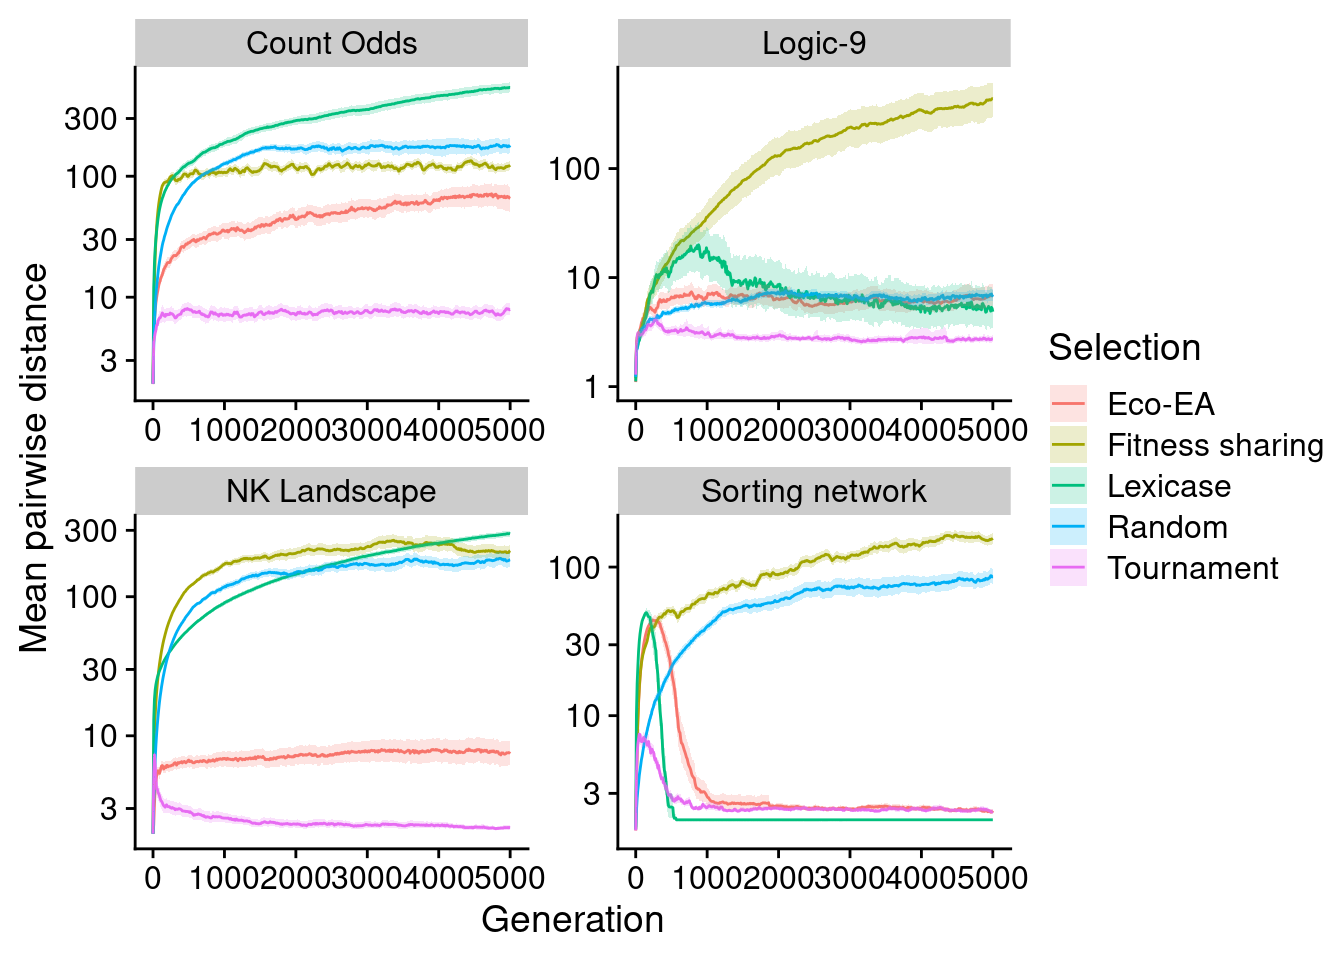
\includegraphics{phylodiversity-in-EC-supplement_files/figure-latex/complex_landscape_phylogeny_over_time_plot-1.pdf}

\hypertarget{final-4}{%
\subsection{Final}\label{final-4}}

\begin{Shaded}
\begin{Highlighting}[]
\CommentTok{# Compute manual labels for geom_signif}
\NormalTok{stat.test <-}\StringTok{ }\NormalTok{final_data }\OperatorTok
\StringTok{  }\KeywordTok{wilcox_test}\NormalTok{(mean_phenotype_pairwise_distance }\OperatorTok{~}\StringTok{ }\NormalTok{selection_name) }\OperatorTok
\StringTok{  }\KeywordTok{adjust_pvalue}\NormalTok{(}\DataTypeTok{method =} \StringTok{"bonferroni"}\NormalTok{) }\OperatorTok
\StringTok{  }\KeywordTok{add_significance}\NormalTok{() }\OperatorTok
\StringTok{  }\KeywordTok{add_xy_position}\NormalTok{(}\DataTypeTok{x=}\StringTok{"selection_name"}\NormalTok{,}\DataTypeTok{step.increase=}\DecValTok{1}\NormalTok{)}
\CommentTok{#stat.test$manual_position <- stat.test$y.position * .5}
\CommentTok{#stat.test$manual_position <- c(110, 150, 170, 170, 130, 110)}
\NormalTok{stat.test}\OperatorTok{$}\NormalTok{label <-}\StringTok{ }\KeywordTok{mapply}\NormalTok{(p_label,stat.test}\OperatorTok{$}\NormalTok{p.adj)}
\end{Highlighting}
\end{Shaded}

\begin{Shaded}
\begin{Highlighting}[]
\KeywordTok{ggplot}\NormalTok{(}
\NormalTok{    final_data,}
    \KeywordTok{aes}\NormalTok{(}
      \DataTypeTok{x=}\NormalTok{selection_name,}
      \DataTypeTok{y=}\NormalTok{mean_phenotype_pairwise_distance,}
      \DataTypeTok{fill=}\NormalTok{selection_name}
\NormalTok{    )}
\NormalTok{  ) }\OperatorTok{+}
\StringTok{  }\KeywordTok{geom_boxplot}\NormalTok{() }\OperatorTok{+}
\StringTok{  }\KeywordTok{scale_y_log10}\NormalTok{(}
    \DataTypeTok{name=}\StringTok{"Mean pairwise distance"}
\NormalTok{  ) }\OperatorTok{+}
\StringTok{  }\KeywordTok{scale_x_discrete}\NormalTok{(}
    \DataTypeTok{name=}\StringTok{"Selection"}
\NormalTok{  ) }\OperatorTok{+}
\StringTok{  }\KeywordTok{scale_fill_discrete}\NormalTok{(}
    \DataTypeTok{name=}\StringTok{"Selection"}
\NormalTok{  ) }\OperatorTok{+}
\StringTok{  }\KeywordTok{scale_color_discrete}\NormalTok{(}
    \DataTypeTok{name=}\StringTok{"Selection"}
\NormalTok{  ) }\OperatorTok{+}\StringTok{ }
\StringTok{  }\KeywordTok{theme}\NormalTok{(}\DataTypeTok{legend.position =} \StringTok{"none"}\NormalTok{) }\OperatorTok{+}
\StringTok{    }\KeywordTok{facet_wrap}\NormalTok{(}\OperatorTok{~}\NormalTok{problem_name, }\DataTypeTok{scales =} \StringTok{"free"}\NormalTok{)}
\end{Highlighting}
\end{Shaded}

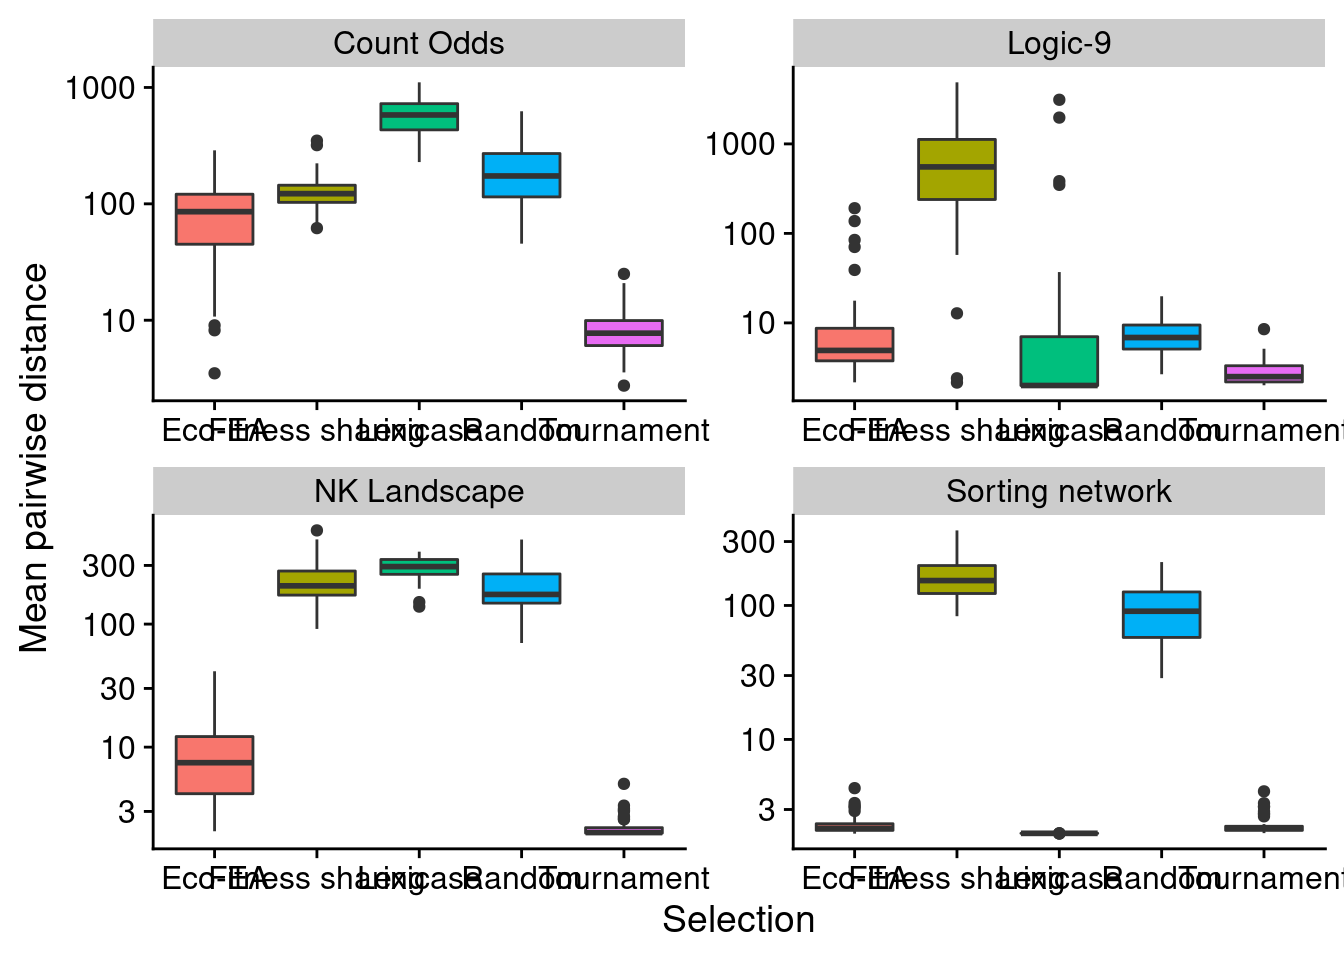
\includegraphics{phylodiversity-in-EC-supplement_files/figure-latex/complex_landscape_final_phylogeny_plot-1.pdf}

\begin{Shaded}
\begin{Highlighting}[]
\NormalTok{stat.test }\OperatorTok
\StringTok{  }\KeywordTok{kbl}\NormalTok{() }\OperatorTok
\StringTok{  }\KeywordTok{kable_styling}\NormalTok{(}
    \DataTypeTok{bootstrap_options =} \KeywordTok{c}\NormalTok{(}
      \StringTok{"striped"}\NormalTok{,}
      \StringTok{"hover"}\NormalTok{,}
      \StringTok{"condensed"}\NormalTok{,}
      \StringTok{"responsive"}
\NormalTok{    )}
\NormalTok{  ) }\OperatorTok
\StringTok{  }\KeywordTok{scroll_box}\NormalTok{(}\DataTypeTok{width=}\StringTok{"600px"}\NormalTok{)}
\end{Highlighting}
\end{Shaded}

\begin{table}
\centering
\begin{tabular}[t]{l|l|l|r|r|r|r|r|l|r|l|r|r|l}
\hline
.y. & group1 & group2 & n1 & n2 & statistic & p & p.adj & p.adj.signif & y.position & groups & xmin & xmax & label\\
\hline
mean\_phenotype\_pairwise\_distance & Eco-EA & Fitness sharing & 240 & 240 & 2831.0 & 0.00e+00 & 0.000000 & **** & 9718.758 & Eco-EA         , Fitness sharing & 1 & 2 & p < 1e-04\\
\hline
mean\_phenotype\_pairwise\_distance & Eco-EA & Lexicase & 240 & 240 & 25159.0 & 1.70e-02 & 0.170000 & ns & 15104.178 & Eco-EA  , Lexicase & 1 & 3 & p = 0.17\\
\hline
mean\_phenotype\_pairwise\_distance & Eco-EA & Random & 240 & 240 & 9552.0 & 0.00e+00 & 0.000000 & **** & 20489.598 & Eco-EA, Random & 1 & 4 & p < 1e-04\\
\hline
mean\_phenotype\_pairwise\_distance & Eco-EA & Tournament & 240 & 240 & 43052.5 & 0.00e+00 & 0.000000 & **** & 25875.018 & Eco-EA    , Tournament & 1 & 5 & p < 1e-04\\
\hline
mean\_phenotype\_pairwise\_distance & Fitness sharing & Lexicase & 240 & 240 & 33683.0 & 1.00e-03 & 0.010000 & ** & 31260.438 & Fitness sharing, Lexicase & 2 & 3 & p = 0.01\\
\hline
mean\_phenotype\_pairwise\_distance & Fitness sharing & Random & 240 & 240 & 40738.0 & 0.00e+00 & 0.000000 & **** & 36645.858 & Fitness sharing, Random & 2 & 4 & p < 1e-04\\
\hline
mean\_phenotype\_pairwise\_distance & Fitness sharing & Tournament & 240 & 240 & 57314.0 & 0.00e+00 & 0.000000 & **** & 42031.278 & Fitness sharing, Tournament & 2 & 5 & p < 1e-04\\
\hline
mean\_phenotype\_pairwise\_distance & Lexicase & Random & 240 & 240 & 28272.0 & 8.49e-01 & 1.000000 & ns & 47416.698 & Lexicase, Random & 3 & 4 & p = 1\\
\hline
mean\_phenotype\_pairwise\_distance & Lexicase & Tournament & 240 & 240 & 34801.0 & 7.84e-05 & 0.000784 & *** & 52802.118 & Lexicase  , Tournament & 3 & 5 & p = 0.000784\\
\hline
mean\_phenotype\_pairwise\_distance & Random & Tournament & 240 & 240 & 54927.0 & 0.00e+00 & 0.000000 & **** & 58187.538 & Random    , Tournament & 4 & 5 & p < 1e-04\\
\hline
\end{tabular}
\end{table}

\hypertarget{phenotypic-diversity-1}{%
\section{Phenotypic diversity}\label{phenotypic-diversity-1}}

\hypertarget{over-time-5}{%
\subsection{Over time}\label{over-time-5}}

\begin{Shaded}
\begin{Highlighting}[]
\KeywordTok{ggplot}\NormalTok{(}
\NormalTok{    data,}
    \KeywordTok{aes}\NormalTok{(}
      \DataTypeTok{x=}\NormalTok{generation,}
      \DataTypeTok{y=}\NormalTok{phenotype_num_taxa,}
      \DataTypeTok{color=}\NormalTok{selection_name,}
      \DataTypeTok{fill=}\NormalTok{selection_name}
\NormalTok{    )}
\NormalTok{  ) }\OperatorTok{+}
\StringTok{  }\KeywordTok{stat_summary}\NormalTok{(}\DataTypeTok{geom=}\StringTok{"line"}\NormalTok{, }\DataTypeTok{fun=}\NormalTok{mean) }\OperatorTok{+}
\StringTok{  }\KeywordTok{stat_summary}\NormalTok{(}
    \DataTypeTok{geom=}\StringTok{"ribbon"}\NormalTok{,}
    \DataTypeTok{fun.data=}\StringTok{"mean_cl_boot"}\NormalTok{,}
    \DataTypeTok{fun.args=}\KeywordTok{list}\NormalTok{(}\DataTypeTok{conf.int=}\FloatTok{0.95}\NormalTok{),}
    \DataTypeTok{alpha=}\FloatTok{0.2}\NormalTok{,}
    \DataTypeTok{linetype=}\DecValTok{0}
\NormalTok{  ) }\OperatorTok{+}
\StringTok{  }\KeywordTok{scale_y_continuous}\NormalTok{(}
    \DataTypeTok{name=}\StringTok{"Phenotypic richness"}
\NormalTok{  ) }\OperatorTok{+}
\StringTok{  }\KeywordTok{scale_x_continuous}\NormalTok{(}
    \DataTypeTok{name=}\StringTok{"Generation"}
\NormalTok{  ) }\OperatorTok{+}
\StringTok{  }\KeywordTok{scale_color_discrete}\NormalTok{(}\StringTok{"Selection"}\NormalTok{) }\OperatorTok{+}\StringTok{ }
\StringTok{  }\KeywordTok{scale_fill_discrete}\NormalTok{(}\StringTok{"Selection"}\NormalTok{) }\OperatorTok{+}
\StringTok{  }\KeywordTok{facet_wrap}\NormalTok{(}\OperatorTok{~}\NormalTok{problem_name, }\DataTypeTok{scales =} \StringTok{"free"}\NormalTok{)}
\end{Highlighting}
\end{Shaded}

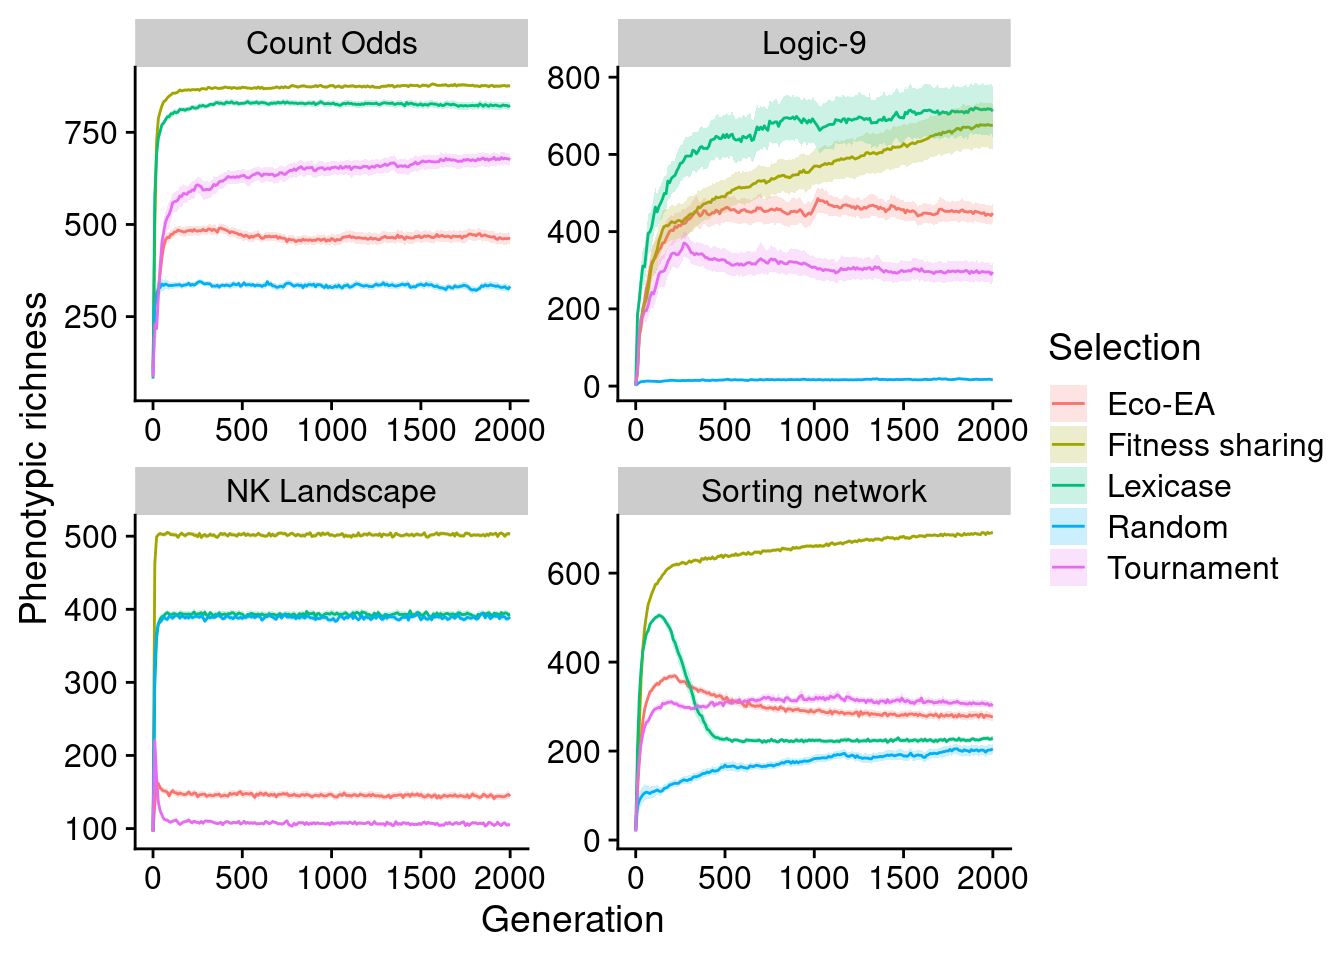
\includegraphics{phylodiversity-in-EC-supplement_files/figure-latex/complex_landscape_phenotypic_diversity_over_time_plot-1.pdf}

\hypertarget{final-5}{%
\subsection{Final}\label{final-5}}

\begin{Shaded}
\begin{Highlighting}[]
\CommentTok{# Compute manual labels for geom_signif}
\NormalTok{stat.test <-}\StringTok{ }\NormalTok{final_data }\OperatorTok
\StringTok{  }\KeywordTok{wilcox_test}\NormalTok{(phenotype_num_taxa }\OperatorTok{~}\StringTok{ }\NormalTok{selection_name) }\OperatorTok
\StringTok{  }\KeywordTok{adjust_pvalue}\NormalTok{(}\DataTypeTok{method =} \StringTok{"bonferroni"}\NormalTok{) }\OperatorTok
\StringTok{  }\KeywordTok{add_significance}\NormalTok{() }\OperatorTok
\StringTok{  }\KeywordTok{add_xy_position}\NormalTok{(}\DataTypeTok{x=}\StringTok{"selection_name"}\NormalTok{,}\DataTypeTok{step.increase=}\DecValTok{1}\NormalTok{)}
\CommentTok{#stat.test$manual_position <- stat.test$y.position * .5}
\CommentTok{#stat.test$manual_position <- c(110, 150, 170, 170, 130, 110)}
\NormalTok{stat.test}\OperatorTok{$}\NormalTok{label <-}\StringTok{ }\KeywordTok{mapply}\NormalTok{(p_label,stat.test}\OperatorTok{$}\NormalTok{p.adj)}
\end{Highlighting}
\end{Shaded}

\begin{Shaded}
\begin{Highlighting}[]
\KeywordTok{ggplot}\NormalTok{(}
\NormalTok{    final_data,}
    \KeywordTok{aes}\NormalTok{(}
      \DataTypeTok{x=}\NormalTok{selection_name,}
      \DataTypeTok{y=}\NormalTok{phenotype_num_taxa,}
      \DataTypeTok{fill=}\NormalTok{selection_name}
\NormalTok{    )}
\NormalTok{  ) }\OperatorTok{+}
\StringTok{  }\KeywordTok{geom_boxplot}\NormalTok{() }\OperatorTok{+}
\StringTok{  }\KeywordTok{scale_y_continuous}\NormalTok{(}
    \DataTypeTok{name=}\StringTok{"Phenotypic Richness"}
\NormalTok{  ) }\OperatorTok{+}
\StringTok{  }\KeywordTok{scale_x_discrete}\NormalTok{(}
    \DataTypeTok{name=}\StringTok{"Selection"}
\NormalTok{  ) }\OperatorTok{+}
\StringTok{  }\KeywordTok{scale_fill_discrete}\NormalTok{(}
    \DataTypeTok{name=}\StringTok{"Selection"}
\NormalTok{  ) }\OperatorTok{+}
\StringTok{  }\KeywordTok{scale_color_discrete}\NormalTok{(}
    \DataTypeTok{name=}\StringTok{"Selection"}
\NormalTok{  ) }\OperatorTok{+}
\StringTok{  }\KeywordTok{theme}\NormalTok{(}\DataTypeTok{legend.position =} \StringTok{"none"}\NormalTok{) }\OperatorTok{+}
\StringTok{  }\KeywordTok{facet_wrap}\NormalTok{(}\OperatorTok{~}\NormalTok{problem_name, }\DataTypeTok{scales =} \StringTok{"free"}\NormalTok{)}
\end{Highlighting}
\end{Shaded}

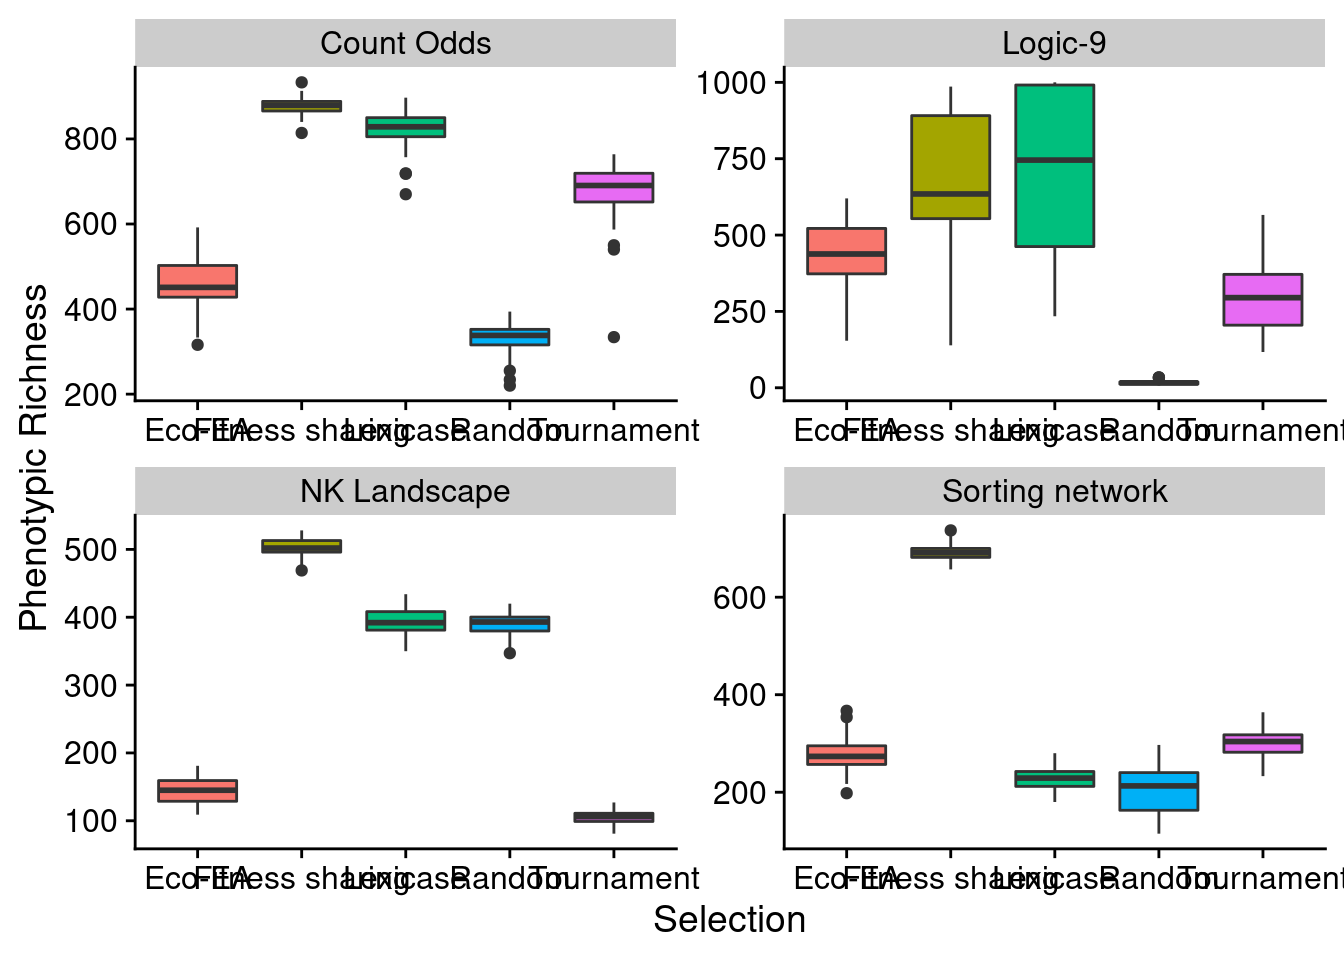
\includegraphics{phylodiversity-in-EC-supplement_files/figure-latex/complex_landscape_final_phenotypic_plot-1.pdf}

\begin{Shaded}
\begin{Highlighting}[]
\NormalTok{stat.test }\OperatorTok
\StringTok{  }\KeywordTok{kbl}\NormalTok{() }\OperatorTok
\StringTok{  }\KeywordTok{kable_styling}\NormalTok{(}
    \DataTypeTok{bootstrap_options =} \KeywordTok{c}\NormalTok{(}
      \StringTok{"striped"}\NormalTok{,}
      \StringTok{"hover"}\NormalTok{,}
      \StringTok{"condensed"}\NormalTok{,}
      \StringTok{"responsive"}
\NormalTok{    )}
\NormalTok{  ) }\OperatorTok
\StringTok{  }\KeywordTok{scroll_box}\NormalTok{(}\DataTypeTok{width=}\StringTok{"600px"}\NormalTok{)}
\end{Highlighting}
\end{Shaded}

\begin{table}
\centering
\begin{tabular}[t]{l|l|l|r|r|r|r|r|l|r|l|r|r|l}
\hline
.y. & group1 & group2 & n1 & n2 & statistic & p & p.adj & p.adj.signif & y.position & groups & xmin & xmax & label\\
\hline
phenotype\_num\_taxa & Eco-EA & Fitness sharing & 240 & 240 & 2406.0 & 0.000000 & 0.00000 & **** & 1507.000 & Eco-EA         , Fitness sharing & 1 & 2 & p < 1e-04\\
\hline
phenotype\_num\_taxa & Eco-EA & Lexicase & 240 & 240 & 14833.5 & 0.000000 & 0.00000 & **** & 2070.333 & Eco-EA  , Lexicase & 1 & 3 & p < 1e-04\\
\hline
phenotype\_num\_taxa & Eco-EA & Random & 240 & 240 & 34261.5 & 0.000326 & 0.00326 & ** & 2633.667 & Eco-EA, Random & 1 & 4 & p = 0.00326\\
\hline
phenotype\_num\_taxa & Eco-EA & Tournament & 240 & 240 & 29587.5 & 0.604000 & 1.00000 & ns & 3197.000 & Eco-EA    , Tournament & 1 & 5 & p = 1\\
\hline
phenotype\_num\_taxa & Fitness sharing & Lexicase & 240 & 240 & 42195.5 & 0.000000 & 0.00000 & **** & 3760.333 & Fitness sharing, Lexicase & 2 & 3 & p < 1e-04\\
\hline
phenotype\_num\_taxa & Fitness sharing & Random & 240 & 240 & 57231.0 & 0.000000 & 0.00000 & **** & 4323.667 & Fitness sharing, Random & 2 & 4 & p < 1e-04\\
\hline
phenotype\_num\_taxa & Fitness sharing & Tournament & 240 & 240 & 51342.0 & 0.000000 & 0.00000 & **** & 4887.000 & Fitness sharing, Tournament & 2 & 5 & p < 1e-04\\
\hline
phenotype\_num\_taxa & Lexicase & Random & 240 & 240 & 47218.0 & 0.000000 & 0.00000 & **** & 5450.333 & Lexicase, Random & 3 & 4 & p < 1e-04\\
\hline
phenotype\_num\_taxa & Lexicase & Tournament & 240 & 240 & 43850.0 & 0.000000 & 0.00000 & **** & 6013.667 & Lexicase  , Tournament & 3 & 5 & p < 1e-04\\
\hline
phenotype\_num\_taxa & Random & Tournament & 240 & 240 & 25692.5 & 0.041000 & 0.41000 & ns & 6577.000 & Random    , Tournament & 4 & 5 & p = 0.41\\
\hline
\end{tabular}
\end{table}

\hypertarget{relationship-between-phenotypic-and-phylogenetic-diversity-1}{%
\section{Relationship between phenotypic and phylogenetic diversity}\label{relationship-between-phenotypic-and-phylogenetic-diversity-1}}

\begin{Shaded}
\begin{Highlighting}[]
\KeywordTok{ggplot}\NormalTok{(}
\NormalTok{    final_data,}
    \KeywordTok{aes}\NormalTok{(}
        \DataTypeTok{y=}\NormalTok{phenotype_num_taxa,}
        \DataTypeTok{x=}\NormalTok{mean_phenotype_pairwise_distance,}
        \DataTypeTok{color=}\NormalTok{selection_name,}
        \DataTypeTok{fill=}\NormalTok{selection_name}
\NormalTok{    )}
\NormalTok{  ) }\OperatorTok{+}
\StringTok{  }\KeywordTok{geom_point}\NormalTok{() }\OperatorTok{+}
\StringTok{    }\KeywordTok{scale_y_continuous}\NormalTok{(}
        \DataTypeTok{name=}\StringTok{"Phenotypic richness"}
\NormalTok{  ) }\OperatorTok{+}
\StringTok{  }\KeywordTok{scale_x_continuous}\NormalTok{(}
        \DataTypeTok{name=}\StringTok{"Mean pairwise distance"}
\NormalTok{  ) }\OperatorTok{+}\StringTok{ }
\StringTok{  }\KeywordTok{facet_wrap}\NormalTok{(}
      \OperatorTok{~}\NormalTok{selection_name}\OperatorTok{*}\NormalTok{problem_name, }\DataTypeTok{scales=}\StringTok{"free"}
\NormalTok{  ) }\OperatorTok{+}\StringTok{ }
\StringTok{  }\KeywordTok{stat_smooth}\NormalTok{(}
    \DataTypeTok{method=}\StringTok{"lm"}
\NormalTok{  ) }\OperatorTok{+}\StringTok{ }
\StringTok{  }\KeywordTok{stat_cor}\NormalTok{(}
    \DataTypeTok{method=}\StringTok{"spearman"}\NormalTok{, }\DataTypeTok{cor.coef.name =} \StringTok{"rho"}\NormalTok{, }\DataTypeTok{color=}\StringTok{"black"}
\NormalTok{  ) }\OperatorTok{+}
\StringTok{  }\KeywordTok{theme}\NormalTok{(}\DataTypeTok{legend.position =} \StringTok{"none"}\NormalTok{)}
\end{Highlighting}
\end{Shaded}

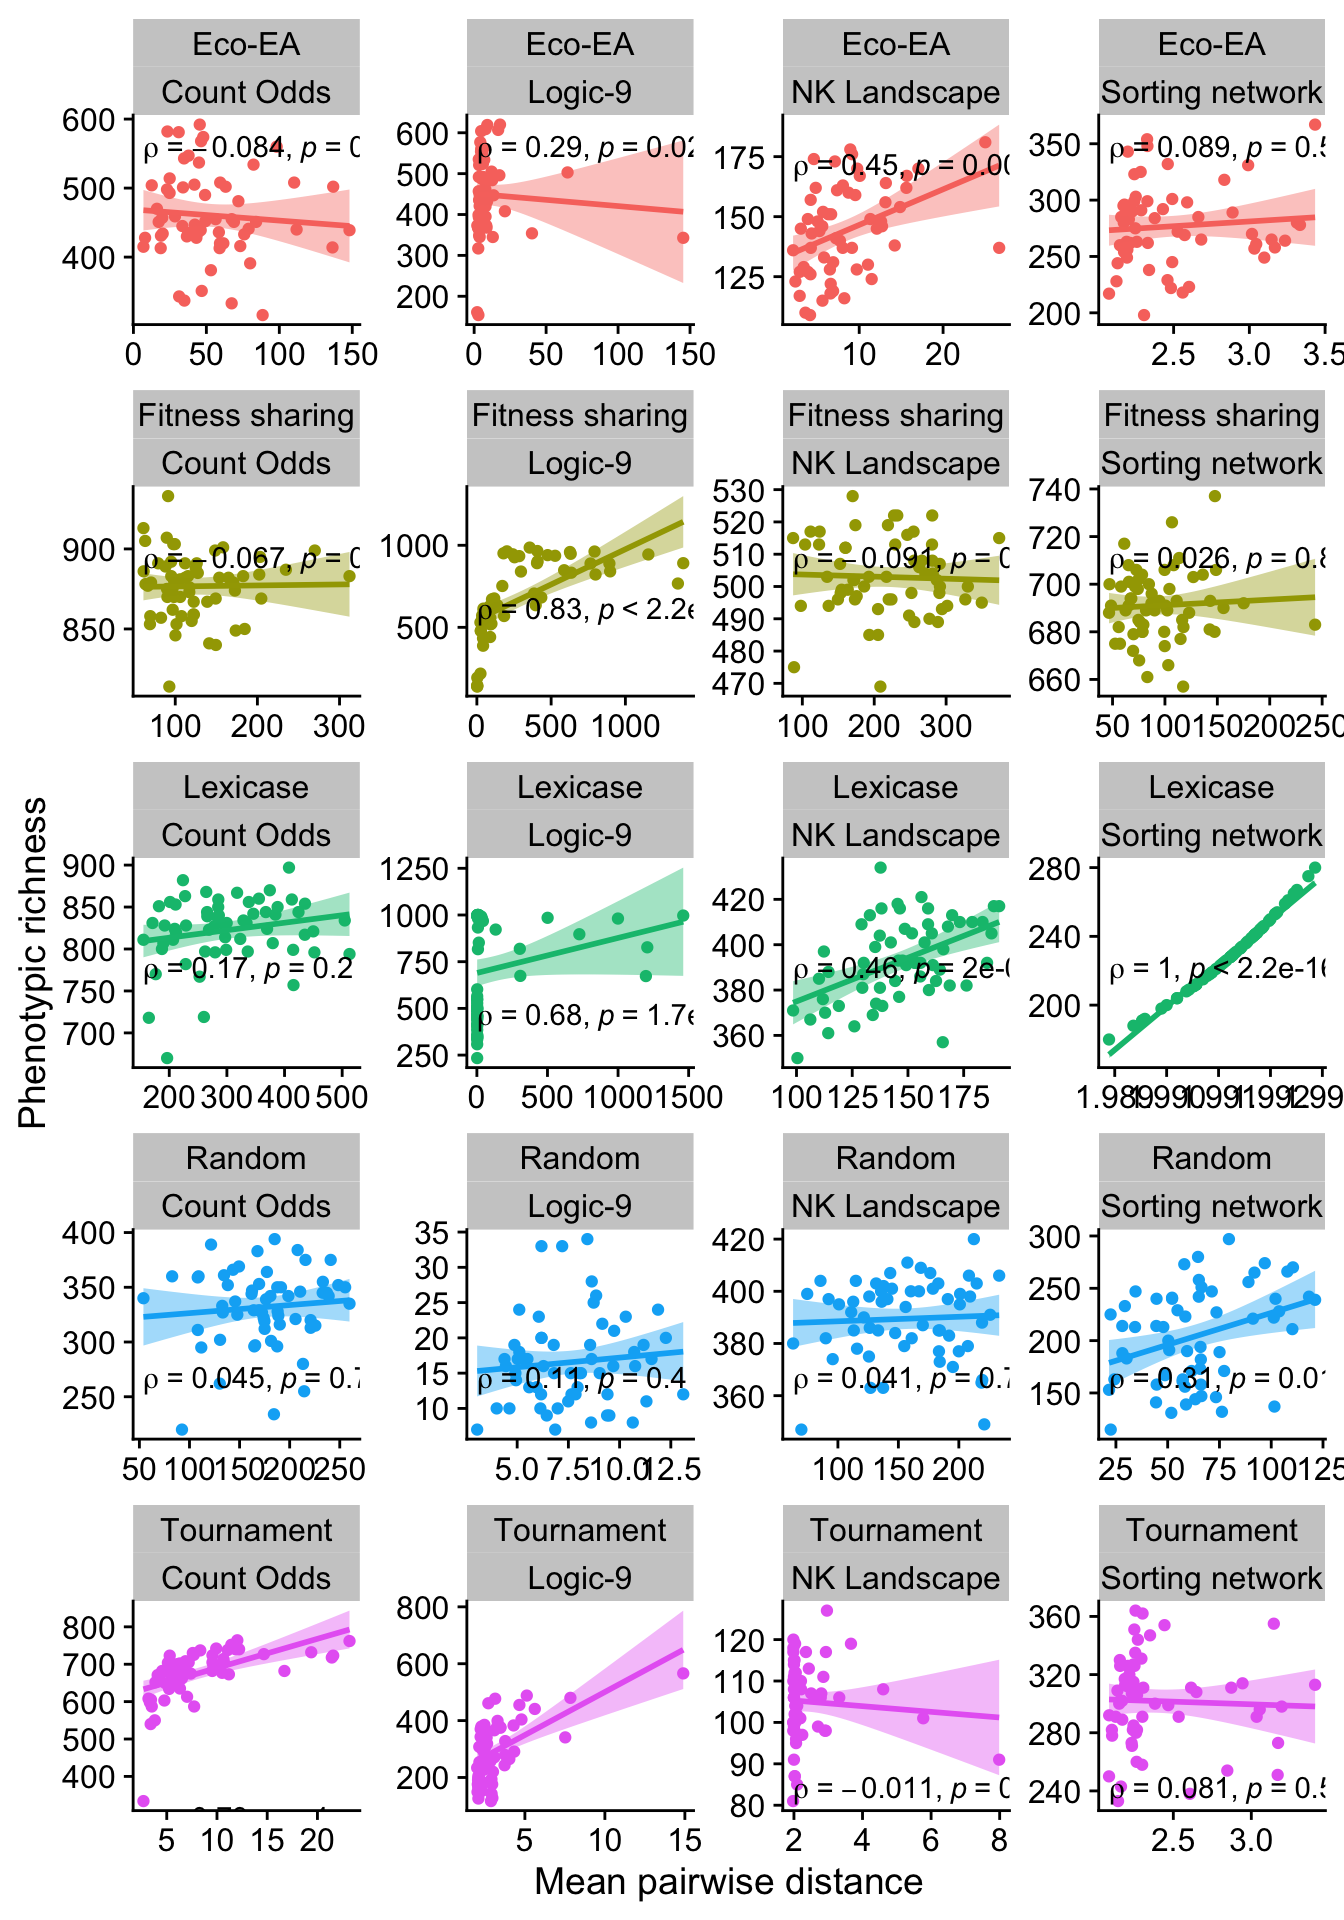
\includegraphics{phylodiversity-in-EC-supplement_files/figure-latex/complex_landscape_phen_vs_phylo-1.pdf}

\hypertarget{relationship-between-diversity-and-success-1}{%
\section{Relationship between diversity and success}\label{relationship-between-diversity-and-success-1}}

\hypertarget{earlier-in-run-1}{%
\subsection{Earlier in run}\label{earlier-in-run-1}}

\begin{Shaded}
\begin{Highlighting}[]
\KeywordTok{ggplot}\NormalTok{(}
\NormalTok{    data }\OperatorTok\StringTok{ }\KeywordTok{filter}\NormalTok{(generation}\OperatorTok{==}\DecValTok{500}\NormalTok{),}
    \KeywordTok{aes}\NormalTok{(}
        \DataTypeTok{y=}\NormalTok{max_performance,}
        \DataTypeTok{x=}\NormalTok{mean_phenotype_pairwise_distance,}
        \DataTypeTok{color=}\NormalTok{selection_name,}
        \DataTypeTok{fill=}\NormalTok{selection_name}
\NormalTok{    )}
\NormalTok{  ) }\OperatorTok{+}
\StringTok{  }\KeywordTok{geom_point}\NormalTok{() }\OperatorTok{+}
\StringTok{    }\KeywordTok{scale_y_continuous}\NormalTok{(}
        \DataTypeTok{name=}\StringTok{"Average trait performance"}
\NormalTok{  ) }\OperatorTok{+}
\StringTok{  }\KeywordTok{scale_x_continuous}\NormalTok{(}
        \DataTypeTok{name=}\StringTok{"Mean pairwise distance"}
\NormalTok{  ) }\OperatorTok{+}\StringTok{ }
\StringTok{  }\KeywordTok{facet_wrap}\NormalTok{(}
      \OperatorTok{~}\NormalTok{selection_name}\OperatorTok{*}\NormalTok{problem_name, }\DataTypeTok{scales=}\StringTok{"free"}
\NormalTok{  ) }\OperatorTok{+}\StringTok{ }
\StringTok{  }\KeywordTok{stat_smooth}\NormalTok{(}
    \DataTypeTok{method=}\StringTok{"lm"}
\NormalTok{  ) }\OperatorTok{+}\StringTok{ }
\StringTok{  }\KeywordTok{stat_cor}\NormalTok{(}
    \DataTypeTok{method=}\StringTok{"spearman"}\NormalTok{, }\DataTypeTok{cor.coef.name =} \StringTok{"rho"}\NormalTok{, }\DataTypeTok{color=}\StringTok{"black"}
\NormalTok{  ) }\OperatorTok{+}
\StringTok{  }\KeywordTok{theme}\NormalTok{(}\DataTypeTok{legend.position =} \StringTok{"none"}\NormalTok{)}
\end{Highlighting}
\end{Shaded}

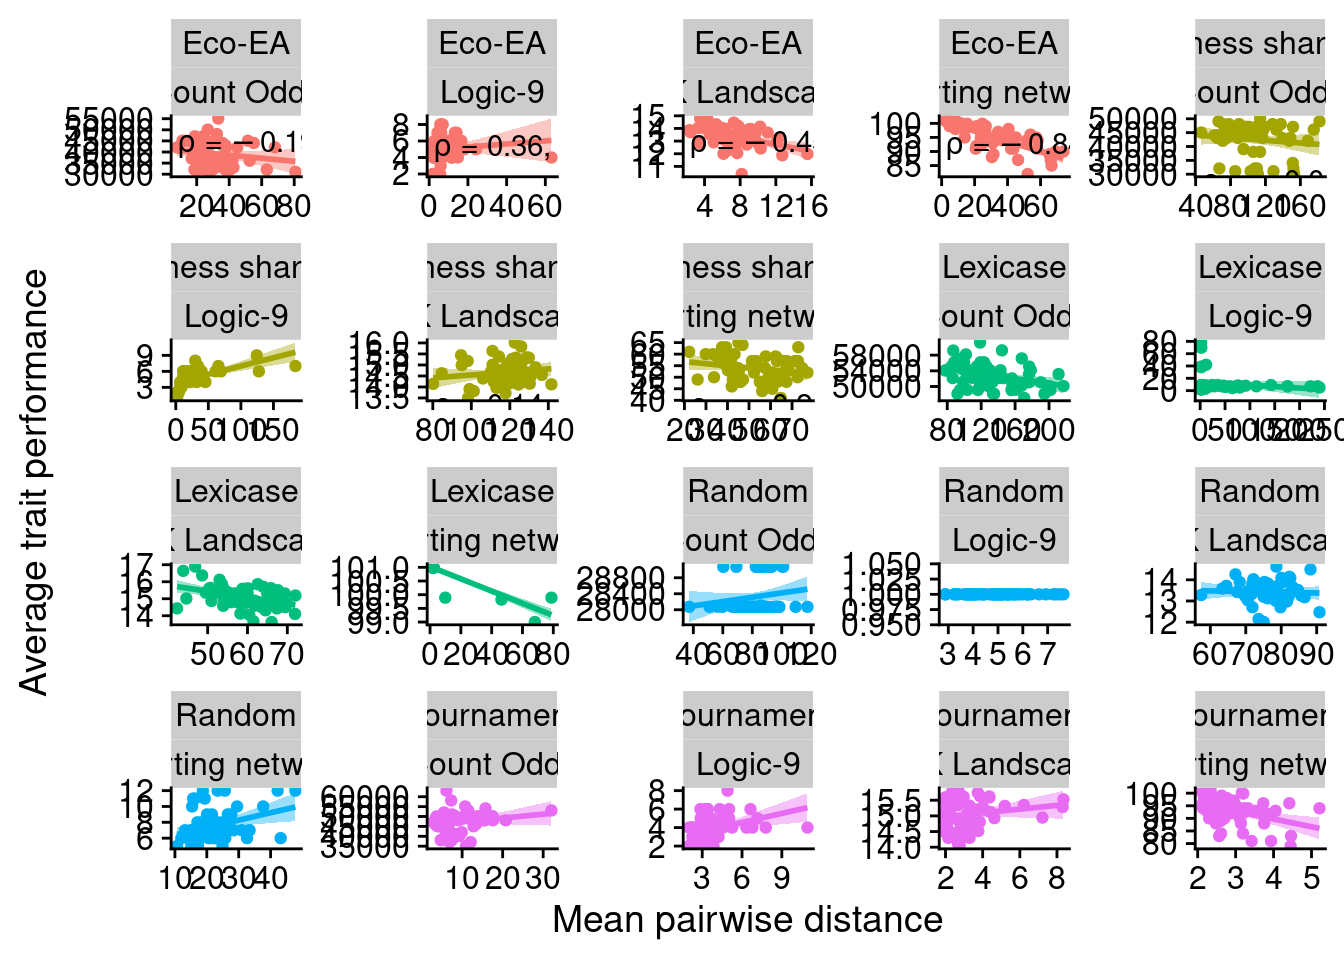
\includegraphics{phylodiversity-in-EC-supplement_files/figure-latex/complex_landscape_phylogeny_vs_performance_very_early-1.pdf}

\begin{Shaded}
\begin{Highlighting}[]
\KeywordTok{ggplot}\NormalTok{(}
\NormalTok{    data }\OperatorTok\StringTok{ }\KeywordTok{filter}\NormalTok{(generation}\OperatorTok{==}\DecValTok{500}\NormalTok{),}
    \KeywordTok{aes}\NormalTok{(}
        \DataTypeTok{y=}\NormalTok{max_performance,}
        \DataTypeTok{x=}\NormalTok{phenotype_num_taxa,}
        \DataTypeTok{color=}\NormalTok{selection_name,}
        \DataTypeTok{fill=}\NormalTok{selection_name}
\NormalTok{    )}
\NormalTok{  ) }\OperatorTok{+}
\StringTok{  }\KeywordTok{geom_point}\NormalTok{() }\OperatorTok{+}
\StringTok{    }\KeywordTok{scale_y_continuous}\NormalTok{(}
        \DataTypeTok{name=}\StringTok{"Average trait performance"}
\NormalTok{  ) }\OperatorTok{+}
\StringTok{  }\KeywordTok{scale_x_continuous}\NormalTok{(}
        \DataTypeTok{name=}\StringTok{"Phenotypic richness"}
\NormalTok{  ) }\OperatorTok{+}\StringTok{ }
\StringTok{  }\KeywordTok{facet_wrap}\NormalTok{(}
      \OperatorTok{~}\NormalTok{selection_name}\OperatorTok{*}\NormalTok{problem_name, }\DataTypeTok{scales=}\StringTok{"free"}
\NormalTok{  ) }\OperatorTok{+}\StringTok{ }
\StringTok{  }\KeywordTok{stat_smooth}\NormalTok{(}
    \DataTypeTok{method=}\StringTok{"lm"}
\NormalTok{  ) }\OperatorTok{+}\StringTok{ }
\StringTok{  }\KeywordTok{stat_cor}\NormalTok{(}
    \DataTypeTok{method=}\StringTok{"spearman"}\NormalTok{, }\DataTypeTok{cor.coef.name =} \StringTok{"rho"}\NormalTok{, }\DataTypeTok{color=}\StringTok{"black"}
\NormalTok{  ) }\OperatorTok{+}
\StringTok{  }\KeywordTok{theme}\NormalTok{(}\DataTypeTok{legend.position =} \StringTok{"none"}\NormalTok{)}
\end{Highlighting}
\end{Shaded}

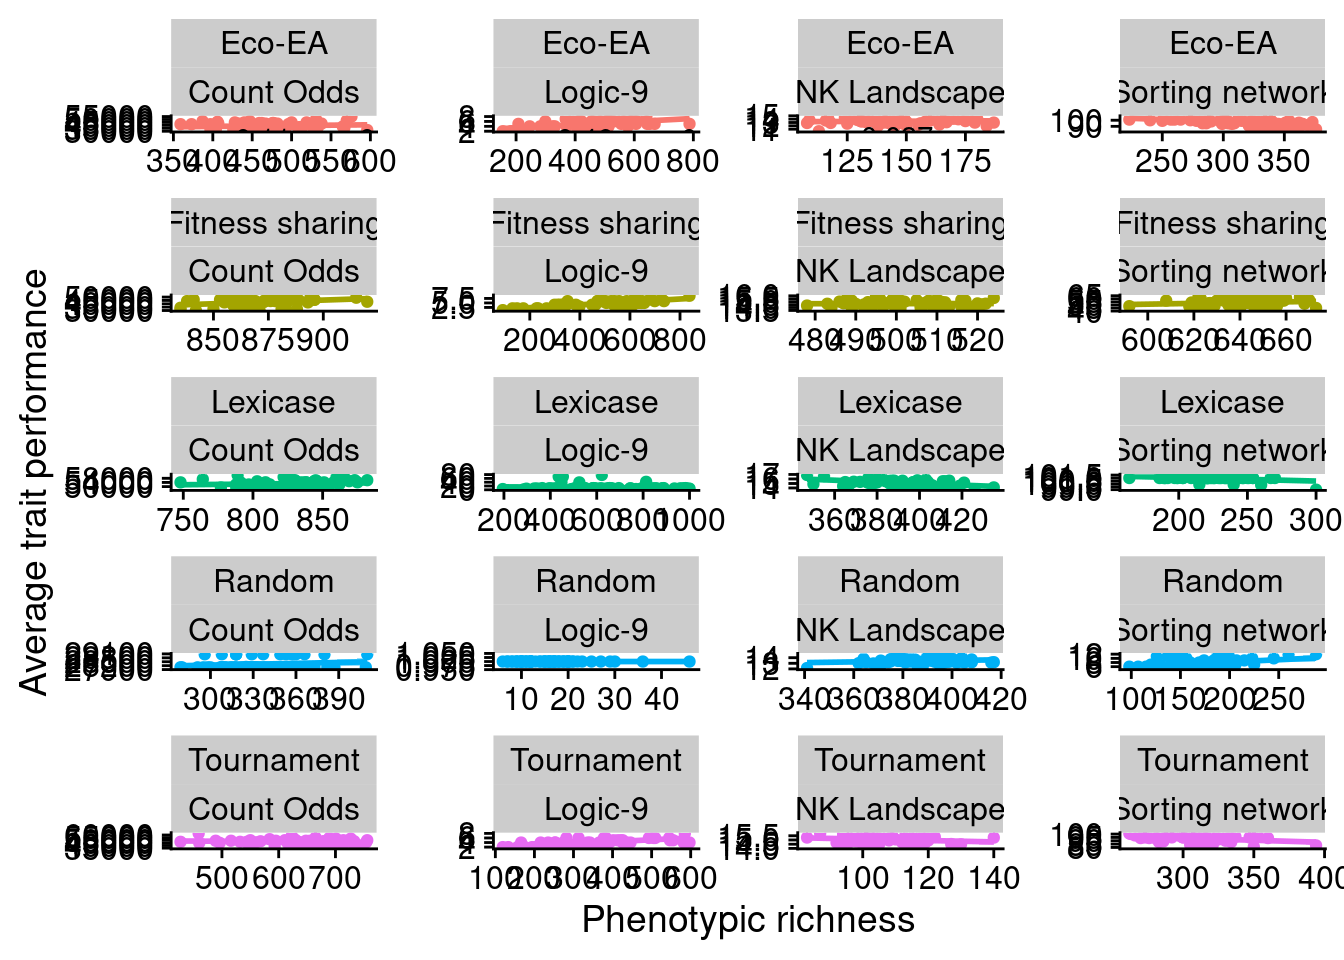
\includegraphics{phylodiversity-in-EC-supplement_files/figure-latex/complex_landscape_richness_vs_performance_very_early-1.pdf}

\begin{Shaded}
\begin{Highlighting}[]
\NormalTok{phylogney_vs_performance <-}\StringTok{ }\KeywordTok{ggplot}\NormalTok{(}
\NormalTok{    data }\OperatorTok\StringTok{ }\KeywordTok{filter}\NormalTok{(generation}\OperatorTok{==}\DecValTok{1000}\NormalTok{),}
    \KeywordTok{aes}\NormalTok{(}
        \DataTypeTok{y=}\NormalTok{max_performance,}
        \DataTypeTok{x=}\NormalTok{mean_phenotype_pairwise_distance,}
        \DataTypeTok{color=}\NormalTok{selection_name,}
        \DataTypeTok{fill=}\NormalTok{selection_name}
\NormalTok{    )}
\NormalTok{  ) }\OperatorTok{+}
\StringTok{  }\KeywordTok{geom_point}\NormalTok{() }\OperatorTok{+}
\StringTok{    }\KeywordTok{scale_y_continuous}\NormalTok{(}
        \DataTypeTok{name=}\StringTok{"Average trait performance"}
\NormalTok{  ) }\OperatorTok{+}
\StringTok{  }\KeywordTok{scale_x_continuous}\NormalTok{(}
        \DataTypeTok{name=}\StringTok{"Mean pairwise distance"}
\NormalTok{  ) }\OperatorTok{+}\StringTok{ }
\StringTok{  }\KeywordTok{facet_wrap}\NormalTok{(}
      \OperatorTok{~}\NormalTok{selection_name}\OperatorTok{*}\NormalTok{problem_name, }\DataTypeTok{scales=}\StringTok{"free"}
\NormalTok{  ) }\OperatorTok{+}\StringTok{ }
\StringTok{  }\KeywordTok{stat_smooth}\NormalTok{(}
    \DataTypeTok{method=}\StringTok{"lm"}
\NormalTok{  ) }\OperatorTok{+}\StringTok{ }
\StringTok{  }\KeywordTok{stat_cor}\NormalTok{(}
    \DataTypeTok{method=}\StringTok{"spearman"}\NormalTok{, }\DataTypeTok{cor.coef.name =} \StringTok{"rho"}\NormalTok{, }\DataTypeTok{color=}\StringTok{"black"}
\NormalTok{  ) }\OperatorTok{+}
\StringTok{  }\KeywordTok{theme}\NormalTok{(}\DataTypeTok{legend.position =} \StringTok{"none"}\NormalTok{)}
  
\NormalTok{phylogney_vs_performance}
\end{Highlighting}
\end{Shaded}

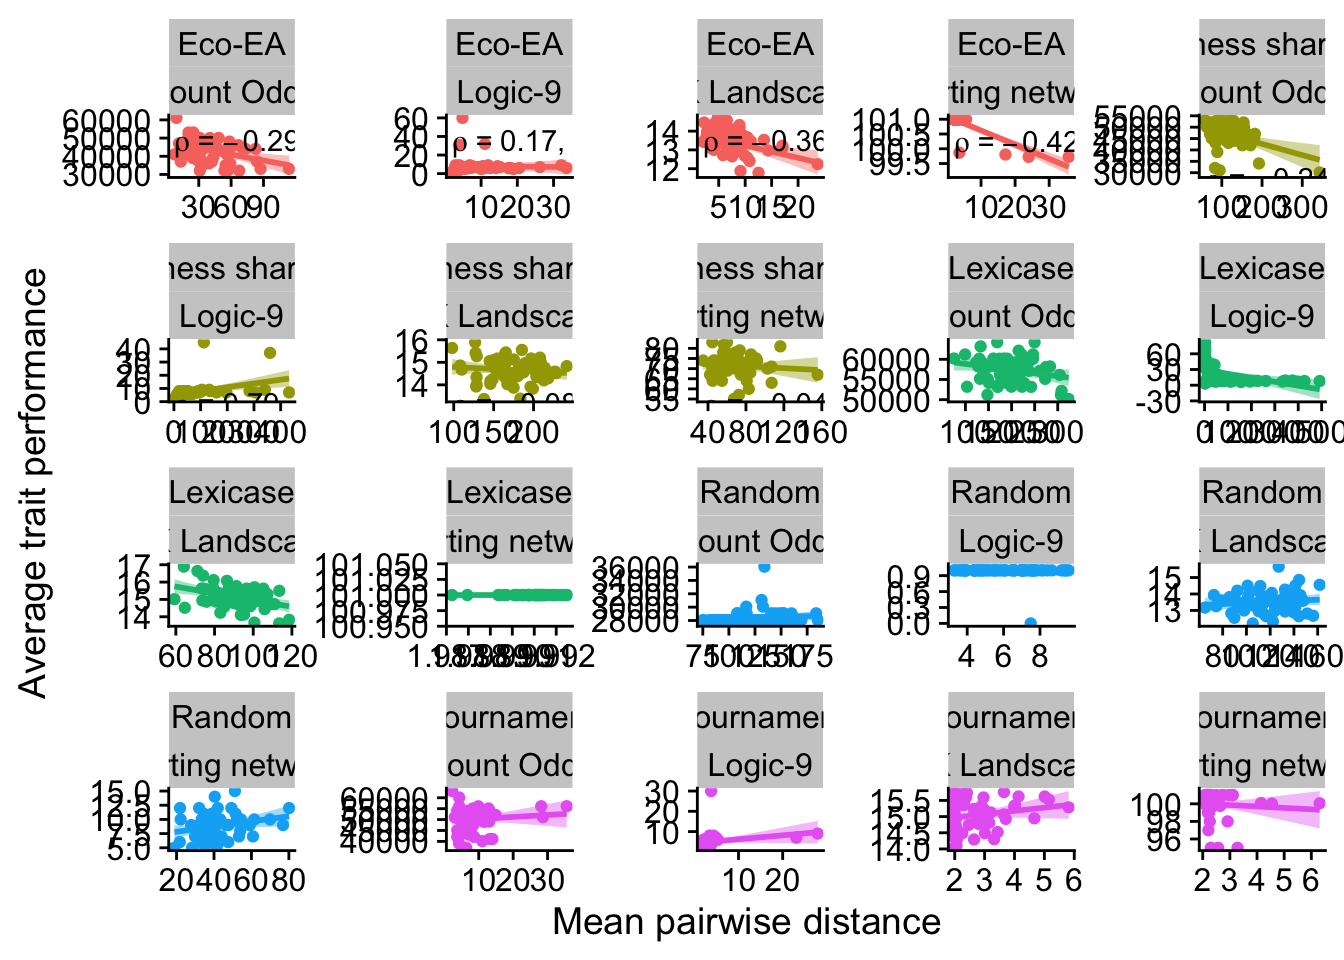
\includegraphics{phylodiversity-in-EC-supplement_files/figure-latex/complex_landscape_phylogeny_vs_performance_early-1.pdf}

\begin{Shaded}
\begin{Highlighting}[]
\KeywordTok{ggplot}\NormalTok{(}
\NormalTok{    data }\OperatorTok\StringTok{ }\KeywordTok{filter}\NormalTok{(generation}\OperatorTok{==}\DecValTok{1000}\NormalTok{),}
    \KeywordTok{aes}\NormalTok{(}
        \DataTypeTok{y=}\NormalTok{max_performance,}
        \DataTypeTok{x=}\NormalTok{phenotype_num_taxa,}
        \DataTypeTok{color=}\NormalTok{selection_name,}
        \DataTypeTok{fill=}\NormalTok{selection_name}
\NormalTok{    )}
\NormalTok{  ) }\OperatorTok{+}
\StringTok{  }\KeywordTok{geom_point}\NormalTok{() }\OperatorTok{+}
\StringTok{    }\KeywordTok{scale_y_continuous}\NormalTok{(}
        \DataTypeTok{name=}\StringTok{"Average trait performance"}
\NormalTok{  ) }\OperatorTok{+}
\StringTok{  }\KeywordTok{scale_x_continuous}\NormalTok{(}
        \DataTypeTok{name=}\StringTok{"Phenotypic richness"}
\NormalTok{  ) }\OperatorTok{+}\StringTok{ }
\StringTok{  }\KeywordTok{facet_wrap}\NormalTok{(}
      \OperatorTok{~}\NormalTok{selection_name}\OperatorTok{*}\NormalTok{problem_name, }\DataTypeTok{scales=}\StringTok{"free"}
\NormalTok{  ) }\OperatorTok{+}\StringTok{ }
\StringTok{  }\KeywordTok{stat_smooth}\NormalTok{(}
    \DataTypeTok{method=}\StringTok{"lm"}
\NormalTok{  ) }\OperatorTok{+}\StringTok{ }
\StringTok{  }\KeywordTok{stat_cor}\NormalTok{(}
    \DataTypeTok{method=}\StringTok{"spearman"}\NormalTok{, }\DataTypeTok{cor.coef.name =} \StringTok{"rho"}\NormalTok{, }\DataTypeTok{color=}\StringTok{"black"}
\NormalTok{  ) }\OperatorTok{+}
\StringTok{  }\KeywordTok{theme}\NormalTok{(}\DataTypeTok{legend.position =} \StringTok{"none"}\NormalTok{)}
\end{Highlighting}
\end{Shaded}

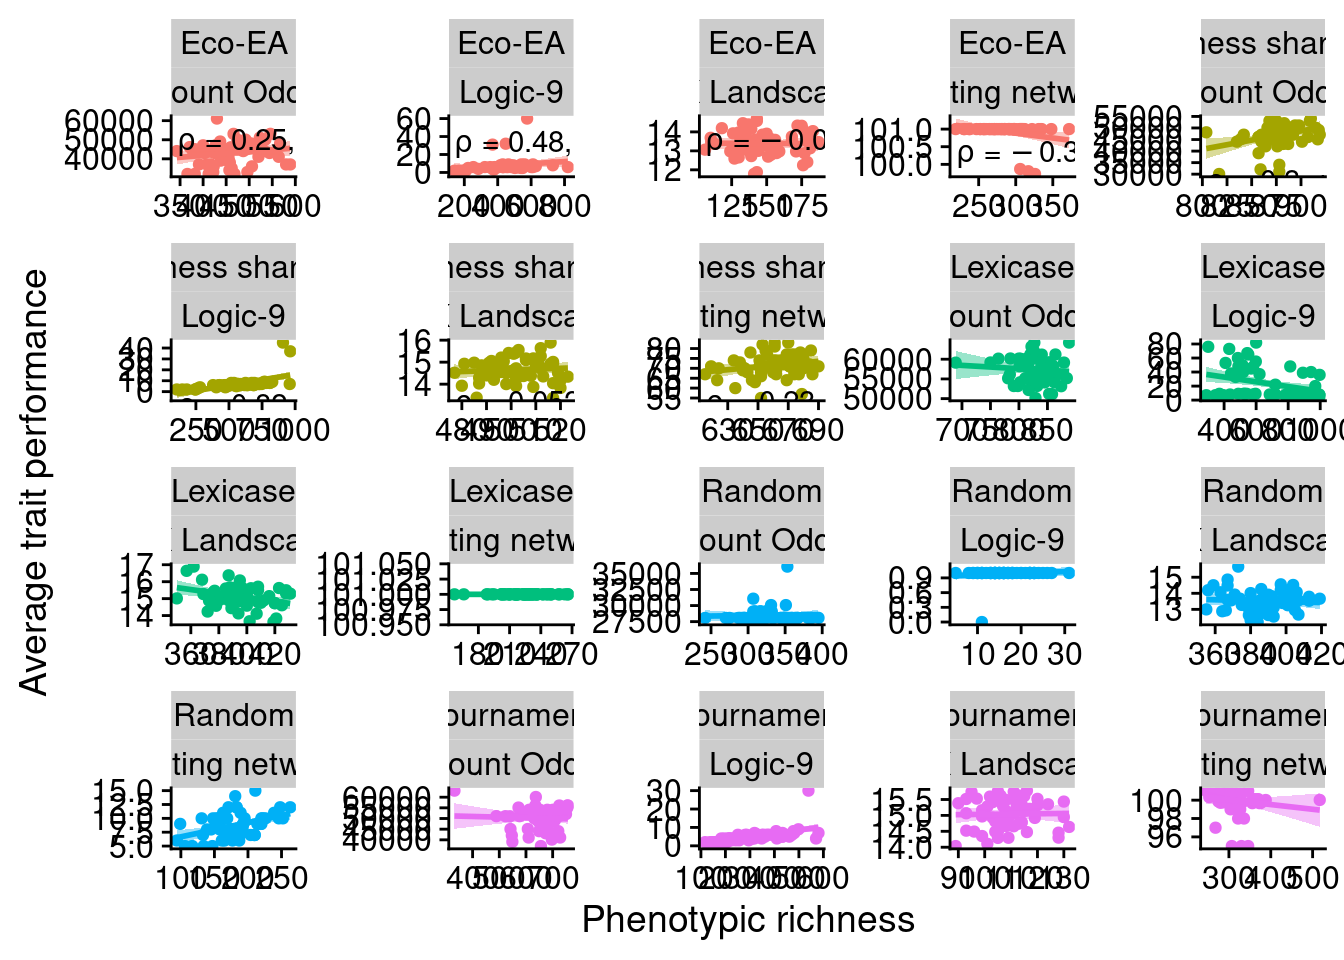
\includegraphics{phylodiversity-in-EC-supplement_files/figure-latex/complex_landscape_richness_vs_performance_early-1.pdf}

\hypertarget{end-of-run-1}{%
\subsection{End of run}\label{end-of-run-1}}

\begin{Shaded}
\begin{Highlighting}[]
\KeywordTok{ggplot}\NormalTok{(}
\NormalTok{    final_data,}
    \KeywordTok{aes}\NormalTok{(}
        \DataTypeTok{y=}\NormalTok{max_performance,}
        \DataTypeTok{x=}\NormalTok{mean_phenotype_pairwise_distance,}
        \DataTypeTok{color=}\NormalTok{selection_name,}
        \DataTypeTok{fill=}\NormalTok{selection_name}
\NormalTok{    )}
\NormalTok{  ) }\OperatorTok{+}
\StringTok{  }\KeywordTok{geom_point}\NormalTok{() }\OperatorTok{+}
\StringTok{    }\KeywordTok{scale_y_continuous}\NormalTok{(}
        \DataTypeTok{name=}\StringTok{"Average trait performance"}
\NormalTok{  ) }\OperatorTok{+}
\StringTok{  }\KeywordTok{scale_x_continuous}\NormalTok{(}
        \DataTypeTok{name=}\StringTok{"Mean pairwise distance"}
\NormalTok{  ) }\OperatorTok{+}\StringTok{ }
\StringTok{  }\KeywordTok{facet_wrap}\NormalTok{(}
      \OperatorTok{~}\NormalTok{selection_name}\OperatorTok{*}\NormalTok{problem_name, }\DataTypeTok{scales=}\StringTok{"free"}
\NormalTok{  ) }\OperatorTok{+}\StringTok{ }
\StringTok{  }\KeywordTok{stat_smooth}\NormalTok{(}
    \DataTypeTok{method=}\StringTok{"lm"}
\NormalTok{  ) }\OperatorTok{+}\StringTok{ }
\StringTok{  }\KeywordTok{stat_cor}\NormalTok{(}
    \DataTypeTok{method=}\StringTok{"spearman"}\NormalTok{, }\DataTypeTok{cor.coef.name =} \StringTok{"rho"}\NormalTok{, }\DataTypeTok{color=}\StringTok{"black"}
\NormalTok{  ) }\OperatorTok{+}
\StringTok{  }\KeywordTok{theme}\NormalTok{(}\DataTypeTok{legend.position =} \StringTok{"none"}\NormalTok{)}
\end{Highlighting}
\end{Shaded}

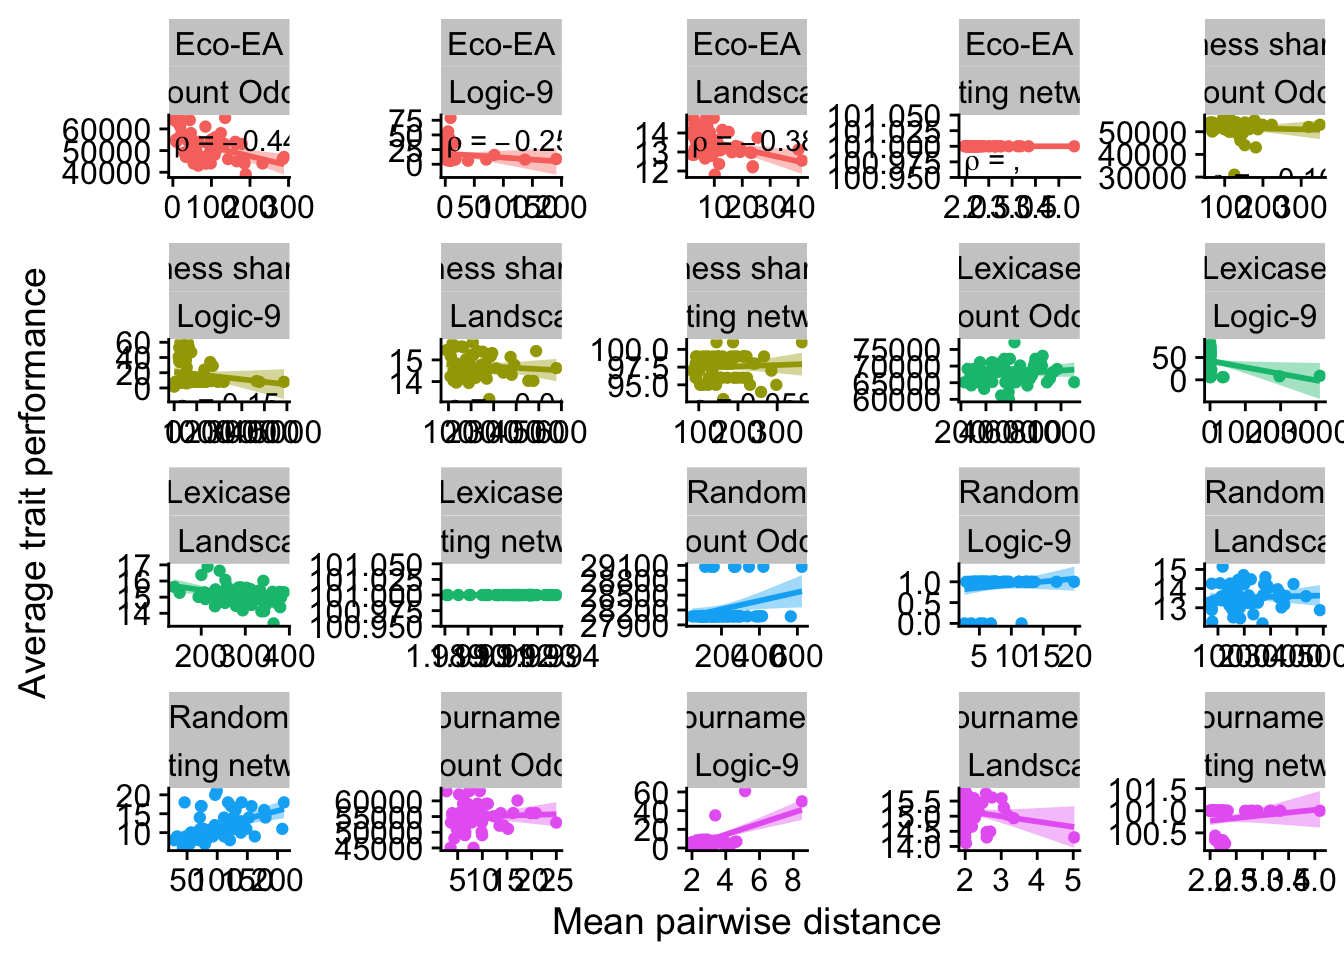
\includegraphics{phylodiversity-in-EC-supplement_files/figure-latex/complex_landscape_phylogeny_vs_performance-1.pdf}

\begin{Shaded}
\begin{Highlighting}[]
\KeywordTok{ggplot}\NormalTok{(}
\NormalTok{    final_data,}
    \KeywordTok{aes}\NormalTok{(}
        \DataTypeTok{y=}\NormalTok{max_performance,}
        \DataTypeTok{x=}\NormalTok{phenotype_num_taxa,}
        \DataTypeTok{color=}\NormalTok{selection_name,}
        \DataTypeTok{fill=}\NormalTok{selection_name}
\NormalTok{    )}
\NormalTok{  ) }\OperatorTok{+}
\StringTok{  }\KeywordTok{geom_point}\NormalTok{() }\OperatorTok{+}
\StringTok{    }\KeywordTok{scale_y_continuous}\NormalTok{(}
        \DataTypeTok{name=}\StringTok{"Average trait performance"}
\NormalTok{  ) }\OperatorTok{+}
\StringTok{  }\KeywordTok{scale_x_continuous}\NormalTok{(}
        \DataTypeTok{name=}\StringTok{"Phenotypic richness"}
\NormalTok{  ) }\OperatorTok{+}\StringTok{ }
\StringTok{  }\KeywordTok{facet_wrap}\NormalTok{(}
      \OperatorTok{~}\NormalTok{selection_name}\OperatorTok{*}\NormalTok{problem_name, }\DataTypeTok{scales=}\StringTok{"free"}
\NormalTok{  ) }\OperatorTok{+}\StringTok{ }
\StringTok{  }\KeywordTok{stat_smooth}\NormalTok{(}
    \DataTypeTok{method=}\StringTok{"lm"}
\NormalTok{  ) }\OperatorTok{+}\StringTok{ }
\StringTok{  }\KeywordTok{stat_cor}\NormalTok{(}
    \DataTypeTok{method=}\StringTok{"spearman"}\NormalTok{, }\DataTypeTok{cor.coef.name =} \StringTok{"rho"}\NormalTok{, }\DataTypeTok{color=}\StringTok{"black"}
\NormalTok{  ) }\OperatorTok{+}
\StringTok{  }\KeywordTok{theme}\NormalTok{(}\DataTypeTok{legend.position =} \StringTok{"none"}\NormalTok{)}
\end{Highlighting}
\end{Shaded}

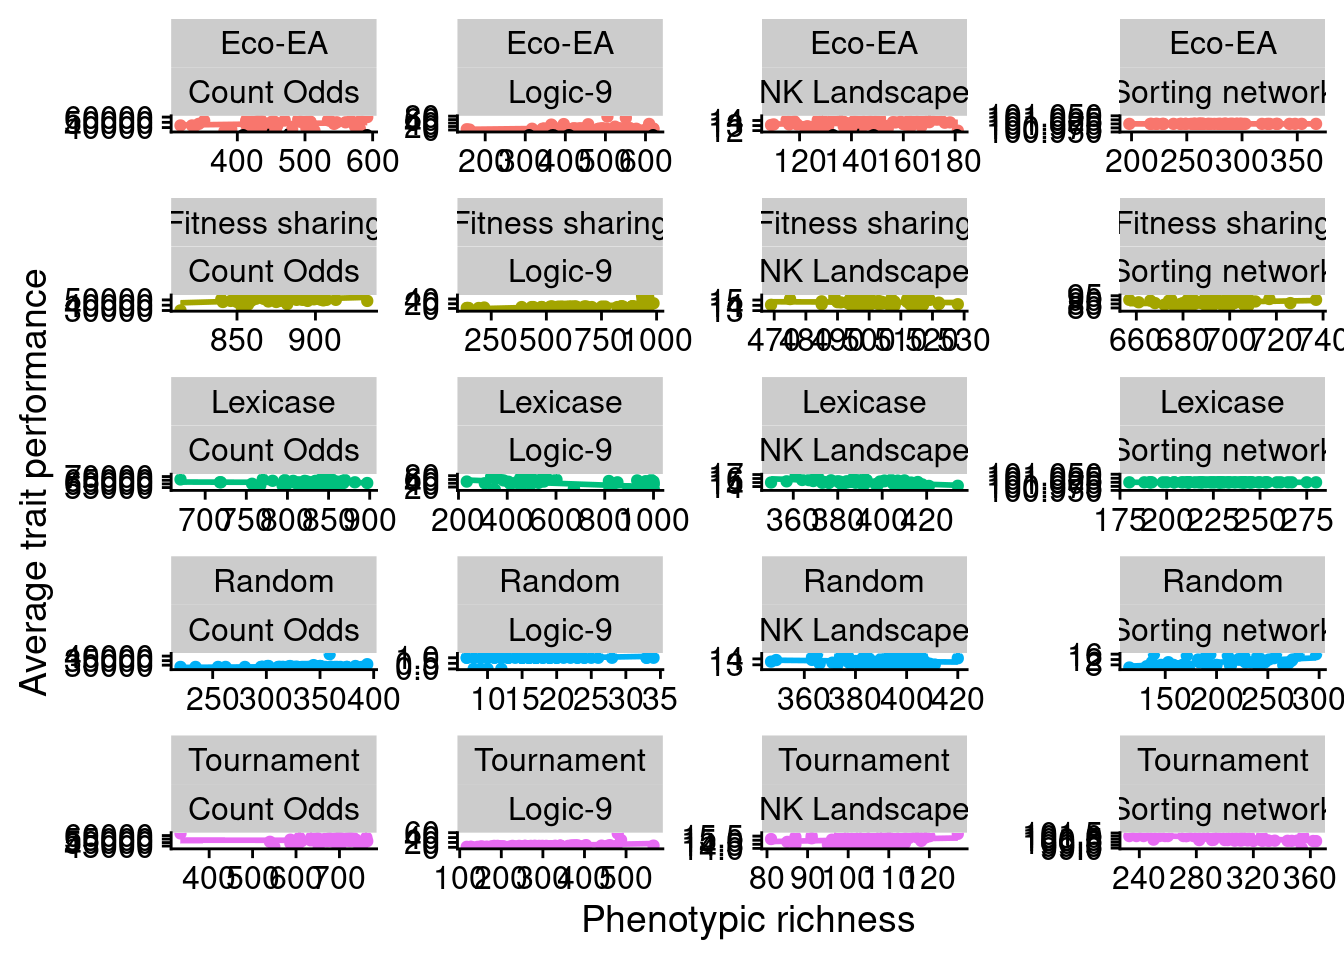
\includegraphics{phylodiversity-in-EC-supplement_files/figure-latex/complex_landscape_richness_vs_performance-1.pdf}

\hypertarget{causality-analysis-1}{%
\section{Causality analysis}\label{causality-analysis-1}}

\begin{Shaded}
\begin{Highlighting}[]
\NormalTok{res <-}\StringTok{ }\NormalTok{data }\OperatorTok\StringTok{ }\KeywordTok{group_by}\NormalTok{(SEED, selection_name, problem_name) }\OperatorTok
\KeywordTok{summarise}\NormalTok{(}
  \DataTypeTok{fit_phylo_10 =} \KeywordTok{condinformation}\NormalTok{(}\KeywordTok{discretize}\NormalTok{(max_performance), }\KeywordTok{discretize}\NormalTok{(}\KeywordTok{lag}\NormalTok{(max_phenotype_pairwise_distance, }\DecValTok{1}\NormalTok{)), }\KeywordTok{discretize}\NormalTok{(}\KeywordTok{lag}\NormalTok{(max_performance, }\DecValTok{1}\NormalTok{))),}
  \DataTypeTok{fit_phylo_100 =} \KeywordTok{condinformation}\NormalTok{(}\KeywordTok{discretize}\NormalTok{(max_performance), }\KeywordTok{discretize}\NormalTok{(}\KeywordTok{lag}\NormalTok{(max_phenotype_pairwise_distance, }\DecValTok{10}\NormalTok{)), }\KeywordTok{discretize}\NormalTok{(}\KeywordTok{lag}\NormalTok{(max_performance, }\DecValTok{10}\NormalTok{))),}
  \DataTypeTok{fit_phylo_1000 =} \KeywordTok{condinformation}\NormalTok{(}\KeywordTok{discretize}\NormalTok{(max_performance), }\KeywordTok{discretize}\NormalTok{(}\KeywordTok{lag}\NormalTok{(max_phenotype_pairwise_distance, }\DecValTok{100}\NormalTok{)), }\KeywordTok{discretize}\NormalTok{(}\KeywordTok{lag}\NormalTok{(max_performance, }\DecValTok{100}\NormalTok{))),}
    \DataTypeTok{fit_pheno_10 =} \KeywordTok{condinformation}\NormalTok{(}\KeywordTok{discretize}\NormalTok{(max_performance), }\KeywordTok{discretize}\NormalTok{(}\KeywordTok{lag}\NormalTok{(phenotype_num_taxa, }\DecValTok{1}\NormalTok{)), }\KeywordTok{discretize}\NormalTok{(}\KeywordTok{lag}\NormalTok{(max_performance, }\DecValTok{1}\NormalTok{))),}
      \DataTypeTok{fit_pheno_100 =} \KeywordTok{condinformation}\NormalTok{(}\KeywordTok{discretize}\NormalTok{(max_performance), }\KeywordTok{discretize}\NormalTok{(}\KeywordTok{lag}\NormalTok{(phenotype_num_taxa, }\DecValTok{10}\NormalTok{)), }\KeywordTok{discretize}\NormalTok{(}\KeywordTok{lag}\NormalTok{(max_performance, }\DecValTok{10}\NormalTok{))),}
      \DataTypeTok{fit_pheno_1000 =} \KeywordTok{condinformation}\NormalTok{(}\KeywordTok{discretize}\NormalTok{(max_performance), }\KeywordTok{discretize}\NormalTok{(}\KeywordTok{lag}\NormalTok{(phenotype_num_taxa, }\DecValTok{100}\NormalTok{)), }\KeywordTok{discretize}\NormalTok{(}\KeywordTok{lag}\NormalTok{(max_performance, }\DecValTok{100}\NormalTok{)))}
\NormalTok{      )}

\NormalTok{res <-}\StringTok{ }\NormalTok{res }\OperatorTok\StringTok{ }\KeywordTok{pivot_longer}\NormalTok{(}\DataTypeTok{cols=}\KeywordTok{contains}\NormalTok{(}\StringTok{"o_10"}\NormalTok{))}
\NormalTok{res}\OperatorTok{$}\NormalTok{offset <-}\StringTok{ }\KeywordTok{str_extract}\NormalTok{(res}\OperatorTok{$}\NormalTok{name, }\StringTok{"[:digit:]*$"}\NormalTok{)}
\NormalTok{res}\OperatorTok{$}\NormalTok{Type <-}\StringTok{ }\KeywordTok{case_when}\NormalTok{(}\KeywordTok{str_detect}\NormalTok{(res}\OperatorTok{$}\NormalTok{name, }\StringTok{"phylo"}\NormalTok{) }\OperatorTok{~}\StringTok{ "Phylogenetic"}\NormalTok{, }\OtherTok{TRUE} \OperatorTok{~}\StringTok{ "Phenotypic"}\NormalTok{)}

\KeywordTok{ggplot}\NormalTok{(}
\NormalTok{  res }\OperatorTok\StringTok{ }\KeywordTok{filter}\NormalTok{(}\KeywordTok{str_detect}\NormalTok{(name, }\StringTok{"fit_ph*"}\NormalTok{)), }
  \KeywordTok{aes}\NormalTok{(}
    \DataTypeTok{x=}\KeywordTok{as.factor}\NormalTok{(offset), }
    \DataTypeTok{y=}\NormalTok{value, }
    \DataTypeTok{color=}\NormalTok{Type}
\NormalTok{    )}
\NormalTok{  ) }\OperatorTok{+}\StringTok{ }
\StringTok{  }\KeywordTok{geom_boxplot}\NormalTok{() }\OperatorTok{+}\StringTok{ }
\StringTok{  }\KeywordTok{facet_wrap}\NormalTok{(}\OperatorTok{~}\NormalTok{problem_name}\OperatorTok{*}\NormalTok{selection_name) }\OperatorTok{+}\StringTok{ }
\StringTok{  }\KeywordTok{scale_x_discrete}\NormalTok{(}\StringTok{"Lag"}\NormalTok{) }\OperatorTok{+}\StringTok{ }
\StringTok{  }\KeywordTok{scale_y_continuous}\NormalTok{(}\StringTok{"Transfer Entropy"}\NormalTok{) }\OperatorTok{+}\StringTok{ }
\StringTok{  }\KeywordTok{scale_color_discrete}\NormalTok{(}\StringTok{""}\NormalTok{) }\OperatorTok{+}\StringTok{ }
\StringTok{  }\KeywordTok{theme}\NormalTok{(}\DataTypeTok{legend.position =} \StringTok{"bottom"}\NormalTok{)}
\end{Highlighting}
\end{Shaded}

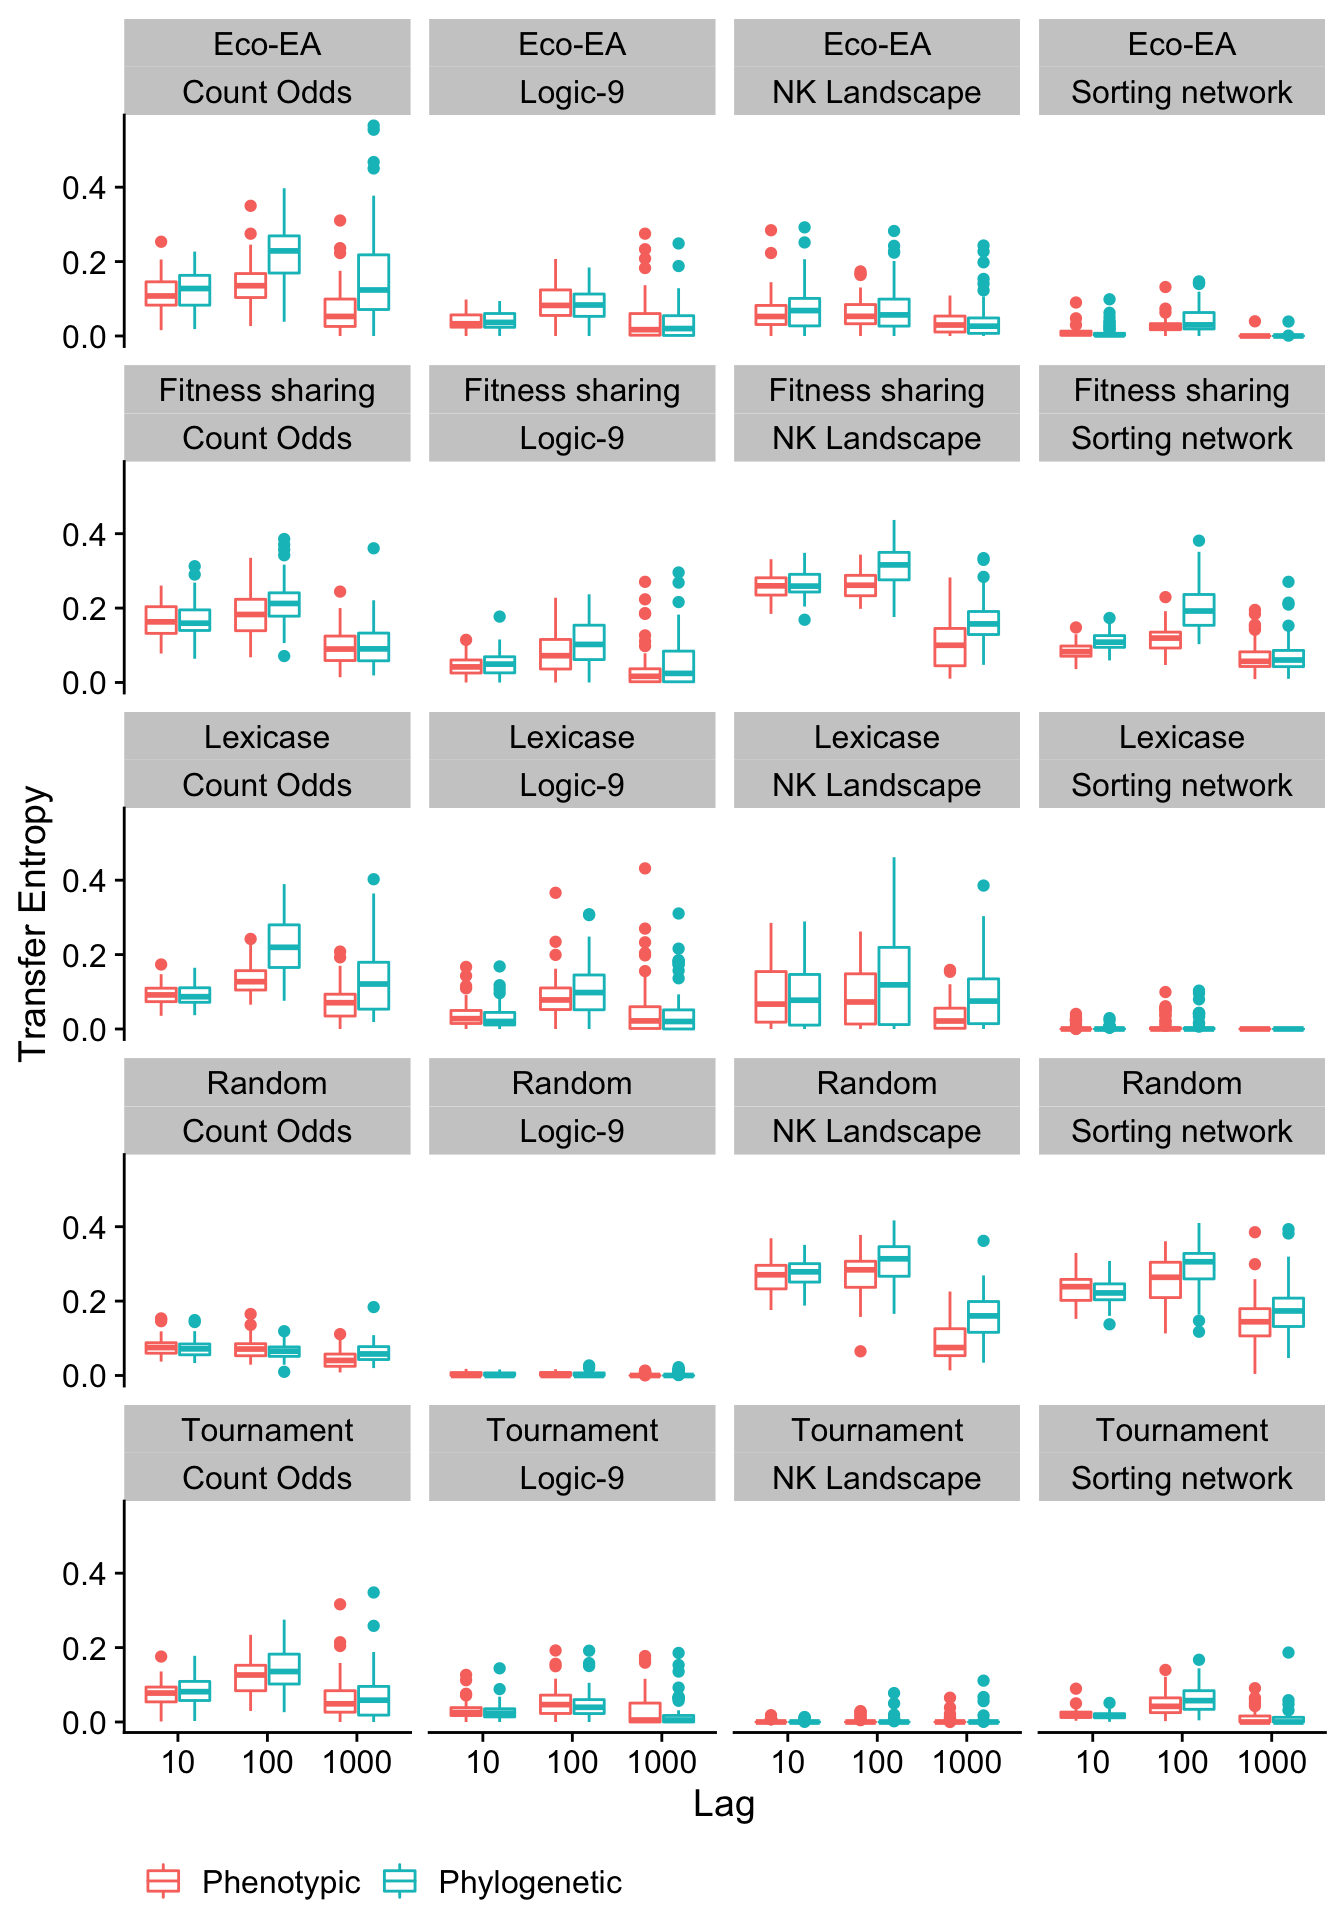
\includegraphics{phylodiversity-in-EC-supplement_files/figure-latex/complex_landscape_information_theory-1.pdf}

\begin{Shaded}
\begin{Highlighting}[]
\NormalTok{res <-}\StringTok{ }\NormalTok{data }\OperatorTok\StringTok{ }\KeywordTok{group_by}\NormalTok{(SEED, selection_name, problem_name) }\OperatorTok
\KeywordTok{summarise}\NormalTok{(}
  \DataTypeTok{fit_phylo_10 =} \KeywordTok{condinformation}\NormalTok{(}\KeywordTok{discretize}\NormalTok{(max_performance), }\KeywordTok{discretize}\NormalTok{(}\KeywordTok{lag}\NormalTok{(mean_phenotype_pairwise_distance, }\DecValTok{1}\NormalTok{)), }\KeywordTok{discretize}\NormalTok{(}\KeywordTok{lag}\NormalTok{(max_performance, }\DecValTok{1}\NormalTok{))),}
  \DataTypeTok{fit_phylo_100 =} \KeywordTok{condinformation}\NormalTok{(}\KeywordTok{discretize}\NormalTok{(max_performance), }\KeywordTok{discretize}\NormalTok{(}\KeywordTok{lag}\NormalTok{(mean_phenotype_pairwise_distance, }\DecValTok{10}\NormalTok{)), }\KeywordTok{discretize}\NormalTok{(}\KeywordTok{lag}\NormalTok{(max_performance, }\DecValTok{10}\NormalTok{))),}
  \DataTypeTok{fit_phylo_1000 =} \KeywordTok{condinformation}\NormalTok{(}\KeywordTok{discretize}\NormalTok{(max_performance), }\KeywordTok{discretize}\NormalTok{(}\KeywordTok{lag}\NormalTok{(mean_phenotype_pairwise_distance, }\DecValTok{100}\NormalTok{)), }\KeywordTok{discretize}\NormalTok{(}\KeywordTok{lag}\NormalTok{(max_performance, }\DecValTok{100}\NormalTok{))),}
    \DataTypeTok{fit_pheno_10 =} \KeywordTok{condinformation}\NormalTok{(}\KeywordTok{discretize}\NormalTok{(max_performance), }\KeywordTok{discretize}\NormalTok{(}\KeywordTok{lag}\NormalTok{(phenotype_num_taxa, }\DecValTok{1}\NormalTok{)), }\KeywordTok{discretize}\NormalTok{(}\KeywordTok{lag}\NormalTok{(max_performance, }\DecValTok{1}\NormalTok{))),}
      \DataTypeTok{fit_pheno_100 =} \KeywordTok{condinformation}\NormalTok{(}\KeywordTok{discretize}\NormalTok{(max_performance), }\KeywordTok{discretize}\NormalTok{(}\KeywordTok{lag}\NormalTok{(phenotype_num_taxa, }\DecValTok{10}\NormalTok{)), }\KeywordTok{discretize}\NormalTok{(}\KeywordTok{lag}\NormalTok{(max_performance, }\DecValTok{10}\NormalTok{))),}
      \DataTypeTok{fit_pheno_1000 =} \KeywordTok{condinformation}\NormalTok{(}\KeywordTok{discretize}\NormalTok{(max_performance), }\KeywordTok{discretize}\NormalTok{(}\KeywordTok{lag}\NormalTok{(phenotype_num_taxa, }\DecValTok{100}\NormalTok{)), }\KeywordTok{discretize}\NormalTok{(}\KeywordTok{lag}\NormalTok{(max_performance, }\DecValTok{100}\NormalTok{)))}
\NormalTok{      )}

\NormalTok{res <-}\StringTok{ }\NormalTok{res }\OperatorTok\StringTok{ }\KeywordTok{pivot_longer}\NormalTok{(}\DataTypeTok{cols=}\KeywordTok{contains}\NormalTok{(}\StringTok{"o_10"}\NormalTok{))}
\NormalTok{res}\OperatorTok{$}\NormalTok{offset <-}\StringTok{ }\KeywordTok{str_extract}\NormalTok{(res}\OperatorTok{$}\NormalTok{name, }\StringTok{"[:digit:]*$"}\NormalTok{)}
\NormalTok{res}\OperatorTok{$}\NormalTok{Type <-}\StringTok{ }\KeywordTok{case_when}\NormalTok{(}\KeywordTok{str_detect}\NormalTok{(res}\OperatorTok{$}\NormalTok{name, }\StringTok{"phylo"}\NormalTok{) }\OperatorTok{~}\StringTok{ "Phylogenetic"}\NormalTok{, }\OtherTok{TRUE} \OperatorTok{~}\StringTok{ "Phenotypic"}\NormalTok{)}

\KeywordTok{ggplot}\NormalTok{(}
\NormalTok{  res }\OperatorTok\StringTok{ }\KeywordTok{filter}\NormalTok{(}\KeywordTok{str_detect}\NormalTok{(name, }\StringTok{"fit_ph*"}\NormalTok{)), }
  \KeywordTok{aes}\NormalTok{(}
    \DataTypeTok{x=}\KeywordTok{as.factor}\NormalTok{(offset), }
    \DataTypeTok{y=}\NormalTok{value, }
    \DataTypeTok{color=}\NormalTok{Type}
\NormalTok{    )}
\NormalTok{  ) }\OperatorTok{+}\StringTok{ }
\StringTok{  }\KeywordTok{geom_boxplot}\NormalTok{() }\OperatorTok{+}\StringTok{ }
\StringTok{  }\KeywordTok{facet_wrap}\NormalTok{(}\OperatorTok{~}\NormalTok{problem_name}\OperatorTok{*}\NormalTok{selection_name) }\OperatorTok{+}\StringTok{ }
\StringTok{  }\KeywordTok{scale_x_discrete}\NormalTok{(}\StringTok{"Lag"}\NormalTok{) }\OperatorTok{+}\StringTok{ }
\StringTok{  }\KeywordTok{scale_y_continuous}\NormalTok{(}\StringTok{"Transfer Entropy"}\NormalTok{) }\OperatorTok{+}\StringTok{ }
\StringTok{  }\KeywordTok{scale_color_discrete}\NormalTok{(}\StringTok{""}\NormalTok{) }\OperatorTok{+}\StringTok{ }
\StringTok{  }\KeywordTok{theme}\NormalTok{(}\DataTypeTok{legend.position =} \StringTok{"bottom"}\NormalTok{)}
\end{Highlighting}
\end{Shaded}

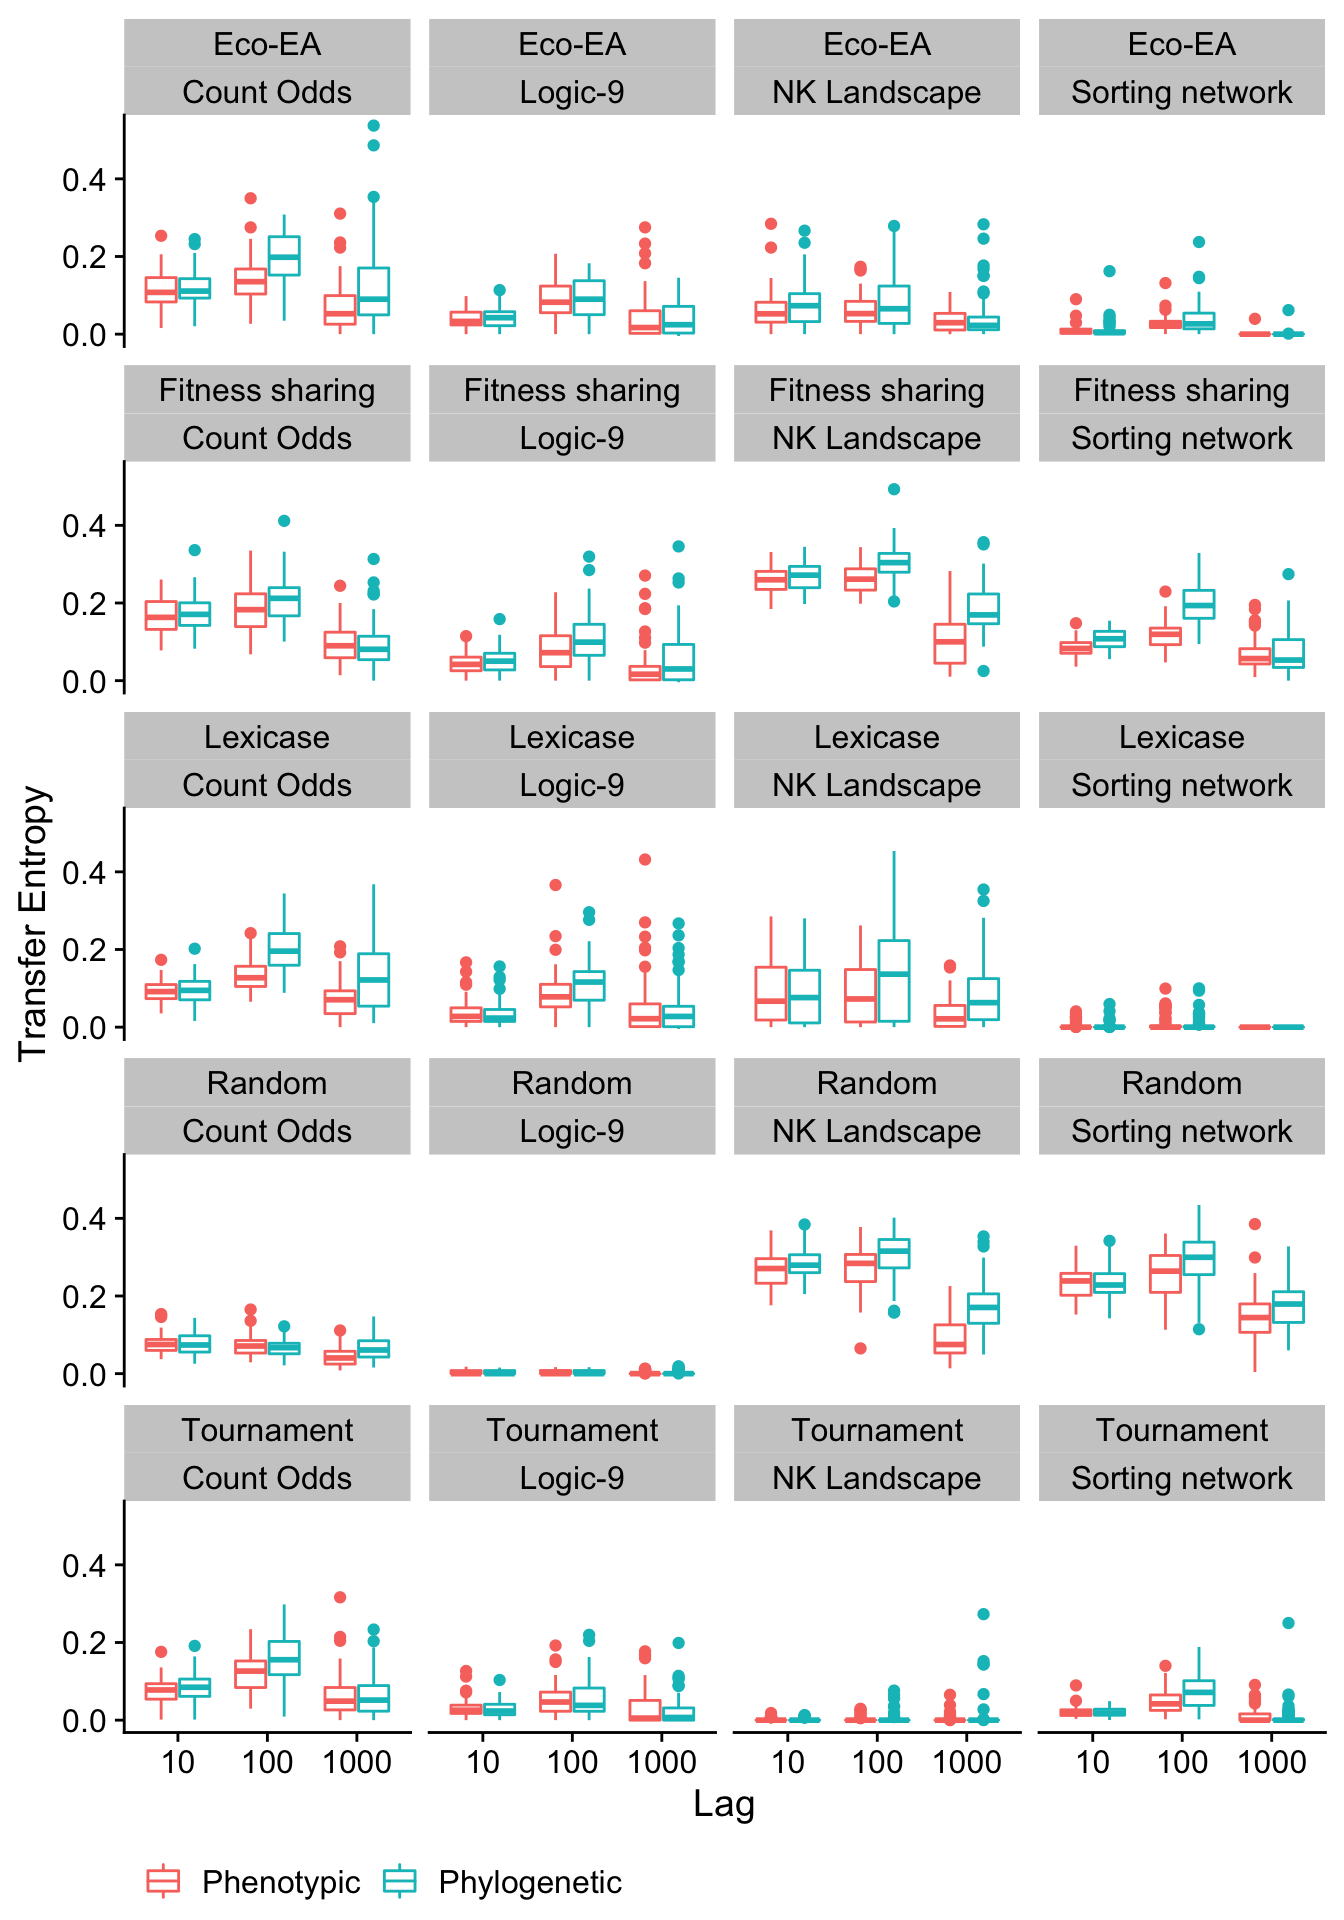
\includegraphics{phylodiversity-in-EC-supplement_files/figure-latex/complex_landscape_information_theory_mpd-1.pdf}

\begin{Shaded}
\begin{Highlighting}[]
\NormalTok{res <-}\StringTok{ }\NormalTok{data }\OperatorTok\StringTok{ }\KeywordTok{group_by}\NormalTok{(SEED, selection_name, problem_name) }\OperatorTok
\KeywordTok{summarise}\NormalTok{(}
  \DataTypeTok{fit_phylo_10 =} \KeywordTok{condinformation}\NormalTok{(}\KeywordTok{discretize}\NormalTok{(max_performance), }\KeywordTok{discretize}\NormalTok{(}\KeywordTok{lag}\NormalTok{(mean_phenotype_evolutionary_distinctiveness, }\DecValTok{1}\NormalTok{)), }\KeywordTok{discretize}\NormalTok{(}\KeywordTok{lag}\NormalTok{(max_performance, }\DecValTok{1}\NormalTok{))),}
  \DataTypeTok{fit_phylo_100 =} \KeywordTok{condinformation}\NormalTok{(}\KeywordTok{discretize}\NormalTok{(max_performance), }\KeywordTok{discretize}\NormalTok{(}\KeywordTok{lag}\NormalTok{(mean_phenotype_evolutionary_distinctiveness, }\DecValTok{10}\NormalTok{)), }\KeywordTok{discretize}\NormalTok{(}\KeywordTok{lag}\NormalTok{(max_performance, }\DecValTok{10}\NormalTok{))),}
  \DataTypeTok{fit_phylo_1000 =} \KeywordTok{condinformation}\NormalTok{(}\KeywordTok{discretize}\NormalTok{(max_performance), }\KeywordTok{discretize}\NormalTok{(}\KeywordTok{lag}\NormalTok{(mean_phenotype_evolutionary_distinctiveness, }\DecValTok{100}\NormalTok{)), }\KeywordTok{discretize}\NormalTok{(}\KeywordTok{lag}\NormalTok{(max_performance, }\DecValTok{100}\NormalTok{))),}
    \DataTypeTok{fit_pheno_10 =} \KeywordTok{condinformation}\NormalTok{(}\KeywordTok{discretize}\NormalTok{(max_performance), }\KeywordTok{discretize}\NormalTok{(}\KeywordTok{lag}\NormalTok{(phenotype_num_taxa, }\DecValTok{1}\NormalTok{)), }\KeywordTok{discretize}\NormalTok{(}\KeywordTok{lag}\NormalTok{(max_performance, }\DecValTok{1}\NormalTok{))),}
      \DataTypeTok{fit_pheno_100 =} \KeywordTok{condinformation}\NormalTok{(}\KeywordTok{discretize}\NormalTok{(max_performance), }\KeywordTok{discretize}\NormalTok{(}\KeywordTok{lag}\NormalTok{(phenotype_num_taxa, }\DecValTok{10}\NormalTok{)), }\KeywordTok{discretize}\NormalTok{(}\KeywordTok{lag}\NormalTok{(max_performance, }\DecValTok{10}\NormalTok{))),}
      \DataTypeTok{fit_pheno_1000 =} \KeywordTok{condinformation}\NormalTok{(}\KeywordTok{discretize}\NormalTok{(max_performance), }\KeywordTok{discretize}\NormalTok{(}\KeywordTok{lag}\NormalTok{(phenotype_num_taxa, }\DecValTok{100}\NormalTok{)), }\KeywordTok{discretize}\NormalTok{(}\KeywordTok{lag}\NormalTok{(max_performance, }\DecValTok{100}\NormalTok{)))}
\NormalTok{      )}

\NormalTok{res <-}\StringTok{ }\NormalTok{res }\OperatorTok\StringTok{ }\KeywordTok{pivot_longer}\NormalTok{(}\DataTypeTok{cols=}\KeywordTok{contains}\NormalTok{(}\StringTok{"o_10"}\NormalTok{))}
\NormalTok{res}\OperatorTok{$}\NormalTok{offset <-}\StringTok{ }\KeywordTok{str_extract}\NormalTok{(res}\OperatorTok{$}\NormalTok{name, }\StringTok{"[:digit:]*$"}\NormalTok{)}
\NormalTok{res}\OperatorTok{$}\NormalTok{Type <-}\StringTok{ }\KeywordTok{case_when}\NormalTok{(}\KeywordTok{str_detect}\NormalTok{(res}\OperatorTok{$}\NormalTok{name, }\StringTok{"phylo"}\NormalTok{) }\OperatorTok{~}\StringTok{ "Phylogenetic"}\NormalTok{, }\OtherTok{TRUE} \OperatorTok{~}\StringTok{ "Phenotypic"}\NormalTok{)}

\KeywordTok{ggplot}\NormalTok{(}
\NormalTok{  res }\OperatorTok\StringTok{ }\KeywordTok{filter}\NormalTok{(}\KeywordTok{str_detect}\NormalTok{(name, }\StringTok{"fit_ph*"}\NormalTok{)), }
  \KeywordTok{aes}\NormalTok{(}
    \DataTypeTok{x=}\KeywordTok{as.factor}\NormalTok{(offset), }
    \DataTypeTok{y=}\NormalTok{value, }
    \DataTypeTok{color=}\NormalTok{Type}
\NormalTok{    )}
\NormalTok{  ) }\OperatorTok{+}\StringTok{ }
\StringTok{  }\KeywordTok{geom_boxplot}\NormalTok{() }\OperatorTok{+}\StringTok{ }
\StringTok{  }\KeywordTok{facet_wrap}\NormalTok{(}\OperatorTok{~}\NormalTok{problem_name}\OperatorTok{*}\NormalTok{selection_name) }\OperatorTok{+}\StringTok{ }
\StringTok{  }\KeywordTok{scale_x_discrete}\NormalTok{(}\StringTok{"Lag"}\NormalTok{) }\OperatorTok{+}\StringTok{ }
\StringTok{  }\KeywordTok{scale_y_continuous}\NormalTok{(}\StringTok{"Transfer Entropy"}\NormalTok{) }\OperatorTok{+}\StringTok{ }
\StringTok{  }\KeywordTok{scale_color_discrete}\NormalTok{(}\StringTok{""}\NormalTok{) }\OperatorTok{+}\StringTok{ }
\StringTok{  }\KeywordTok{theme}\NormalTok{(}\DataTypeTok{legend.position =} \StringTok{"bottom"}\NormalTok{)}
\end{Highlighting}
\end{Shaded}

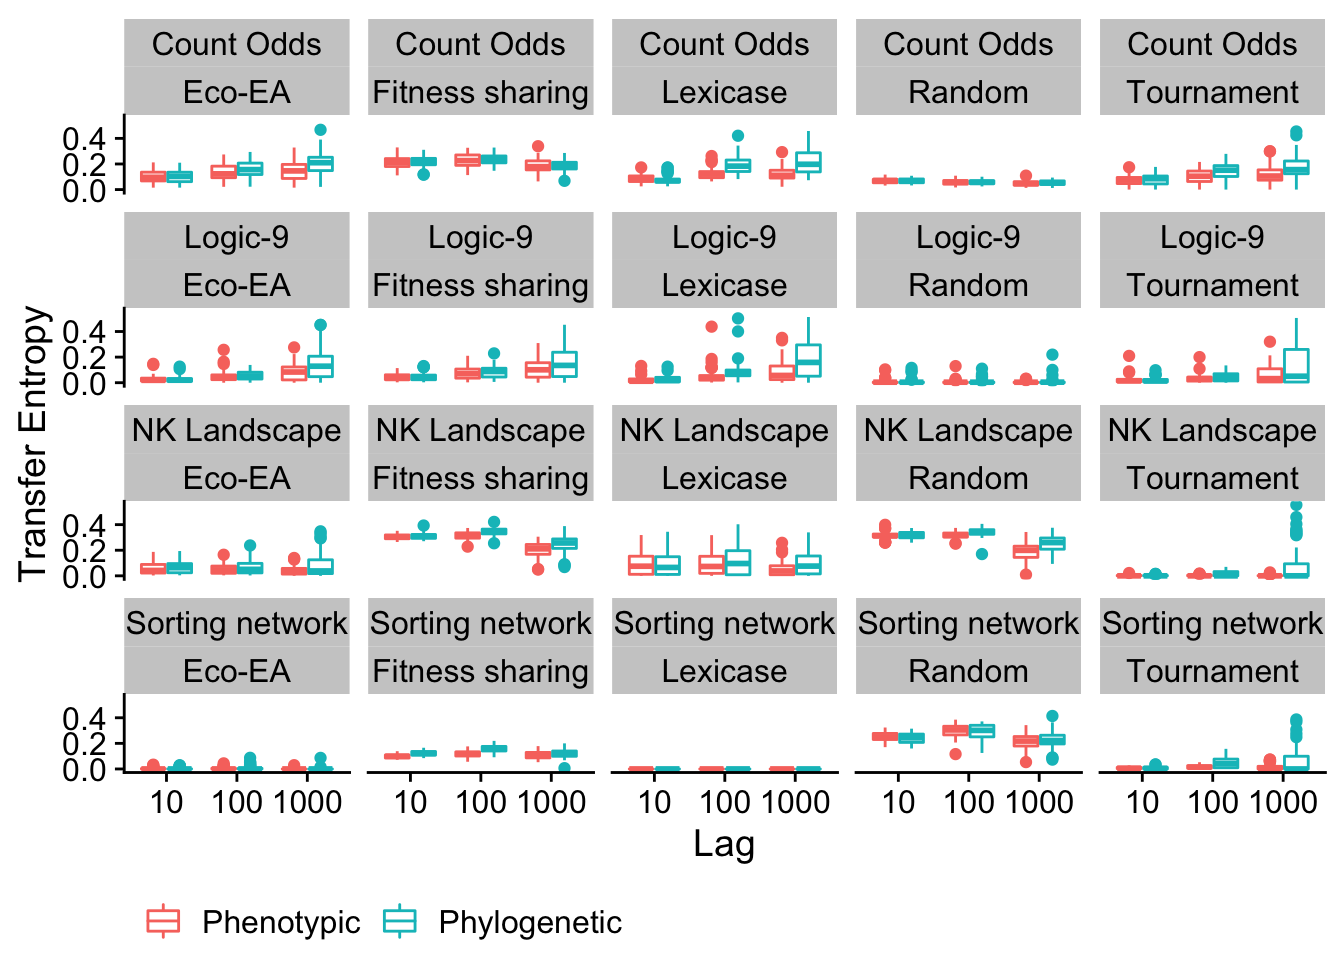
\includegraphics{phylodiversity-in-EC-supplement_files/figure-latex/complex_landscape_information_theory_mean_evolutionary_distinctivess-1.pdf}

\begin{Shaded}
\begin{Highlighting}[]
\NormalTok{res <-}\StringTok{ }\NormalTok{data }\OperatorTok\StringTok{ }\KeywordTok{group_by}\NormalTok{(SEED, selection_name, problem_name) }\OperatorTok
\KeywordTok{summarise}\NormalTok{(}
  \DataTypeTok{fit_phylo_10 =} \KeywordTok{condinformation}\NormalTok{(}\KeywordTok{discretize}\NormalTok{(max_performance), }\KeywordTok{discretize}\NormalTok{(}\KeywordTok{lag}\NormalTok{(variance_phenotype_evolutionary_distinctiveness, }\DecValTok{1}\NormalTok{)), }\KeywordTok{discretize}\NormalTok{(}\KeywordTok{lag}\NormalTok{(max_performance, }\DecValTok{1}\NormalTok{))),}
  \DataTypeTok{fit_phylo_100 =} \KeywordTok{condinformation}\NormalTok{(}\KeywordTok{discretize}\NormalTok{(max_performance), }\KeywordTok{discretize}\NormalTok{(}\KeywordTok{lag}\NormalTok{(variance_phenotype_evolutionary_distinctiveness, }\DecValTok{10}\NormalTok{)), }\KeywordTok{discretize}\NormalTok{(}\KeywordTok{lag}\NormalTok{(max_performance, }\DecValTok{10}\NormalTok{))),}
  \DataTypeTok{fit_phylo_1000 =} \KeywordTok{condinformation}\NormalTok{(}\KeywordTok{discretize}\NormalTok{(max_performance), }\KeywordTok{discretize}\NormalTok{(}\KeywordTok{lag}\NormalTok{(variance_phenotype_evolutionary_distinctiveness, }\DecValTok{100}\NormalTok{)), }\KeywordTok{discretize}\NormalTok{(}\KeywordTok{lag}\NormalTok{(max_performance, }\DecValTok{100}\NormalTok{))),}
    \DataTypeTok{fit_pheno_10 =} \KeywordTok{condinformation}\NormalTok{(}\KeywordTok{discretize}\NormalTok{(max_performance), }\KeywordTok{discretize}\NormalTok{(}\KeywordTok{lag}\NormalTok{(phenotype_num_taxa, }\DecValTok{1}\NormalTok{)), }\KeywordTok{discretize}\NormalTok{(}\KeywordTok{lag}\NormalTok{(max_performance, }\DecValTok{1}\NormalTok{))),}
      \DataTypeTok{fit_pheno_100 =} \KeywordTok{condinformation}\NormalTok{(}\KeywordTok{discretize}\NormalTok{(max_performance), }\KeywordTok{discretize}\NormalTok{(}\KeywordTok{lag}\NormalTok{(phenotype_num_taxa, }\DecValTok{10}\NormalTok{)), }\KeywordTok{discretize}\NormalTok{(}\KeywordTok{lag}\NormalTok{(max_performance, }\DecValTok{10}\NormalTok{))),}
      \DataTypeTok{fit_pheno_1000 =} \KeywordTok{condinformation}\NormalTok{(}\KeywordTok{discretize}\NormalTok{(max_performance), }\KeywordTok{discretize}\NormalTok{(}\KeywordTok{lag}\NormalTok{(phenotype_num_taxa, }\DecValTok{100}\NormalTok{)), }\KeywordTok{discretize}\NormalTok{(}\KeywordTok{lag}\NormalTok{(max_performance, }\DecValTok{100}\NormalTok{)))}
\NormalTok{      )}

\NormalTok{res <-}\StringTok{ }\NormalTok{res }\OperatorTok\StringTok{ }\KeywordTok{pivot_longer}\NormalTok{(}\DataTypeTok{cols=}\KeywordTok{contains}\NormalTok{(}\StringTok{"o_10"}\NormalTok{))}
\NormalTok{res}\OperatorTok{$}\NormalTok{offset <-}\StringTok{ }\KeywordTok{str_extract}\NormalTok{(res}\OperatorTok{$}\NormalTok{name, }\StringTok{"[:digit:]*$"}\NormalTok{)}
\NormalTok{res}\OperatorTok{$}\NormalTok{Type <-}\StringTok{ }\KeywordTok{case_when}\NormalTok{(}\KeywordTok{str_detect}\NormalTok{(res}\OperatorTok{$}\NormalTok{name, }\StringTok{"phylo"}\NormalTok{) }\OperatorTok{~}\StringTok{ "Phylogenetic"}\NormalTok{, }\OtherTok{TRUE} \OperatorTok{~}\StringTok{ "Phenotypic"}\NormalTok{)}

\KeywordTok{ggplot}\NormalTok{(}
\NormalTok{  res }\OperatorTok\StringTok{ }\KeywordTok{filter}\NormalTok{(}\KeywordTok{str_detect}\NormalTok{(name, }\StringTok{"fit_ph*"}\NormalTok{)), }
  \KeywordTok{aes}\NormalTok{(}
    \DataTypeTok{x=}\KeywordTok{as.factor}\NormalTok{(offset), }
    \DataTypeTok{y=}\NormalTok{value, }
    \DataTypeTok{color=}\NormalTok{Type}
\NormalTok{    )}
\NormalTok{  ) }\OperatorTok{+}\StringTok{ }
\StringTok{  }\KeywordTok{geom_boxplot}\NormalTok{() }\OperatorTok{+}\StringTok{ }
\StringTok{  }\KeywordTok{facet_wrap}\NormalTok{(}\OperatorTok{~}\NormalTok{problem_name}\OperatorTok{*}\NormalTok{selection_name) }\OperatorTok{+}\StringTok{ }
\StringTok{  }\KeywordTok{scale_x_discrete}\NormalTok{(}\StringTok{"Lag"}\NormalTok{) }\OperatorTok{+}\StringTok{ }
\StringTok{  }\KeywordTok{scale_y_continuous}\NormalTok{(}\StringTok{"Transfer Entropy"}\NormalTok{) }\OperatorTok{+}\StringTok{ }
\StringTok{  }\KeywordTok{scale_color_discrete}\NormalTok{(}\StringTok{""}\NormalTok{) }\OperatorTok{+}\StringTok{ }
\StringTok{  }\KeywordTok{theme}\NormalTok{(}\DataTypeTok{legend.position =} \StringTok{"bottom"}\NormalTok{)}
\end{Highlighting}
\end{Shaded}

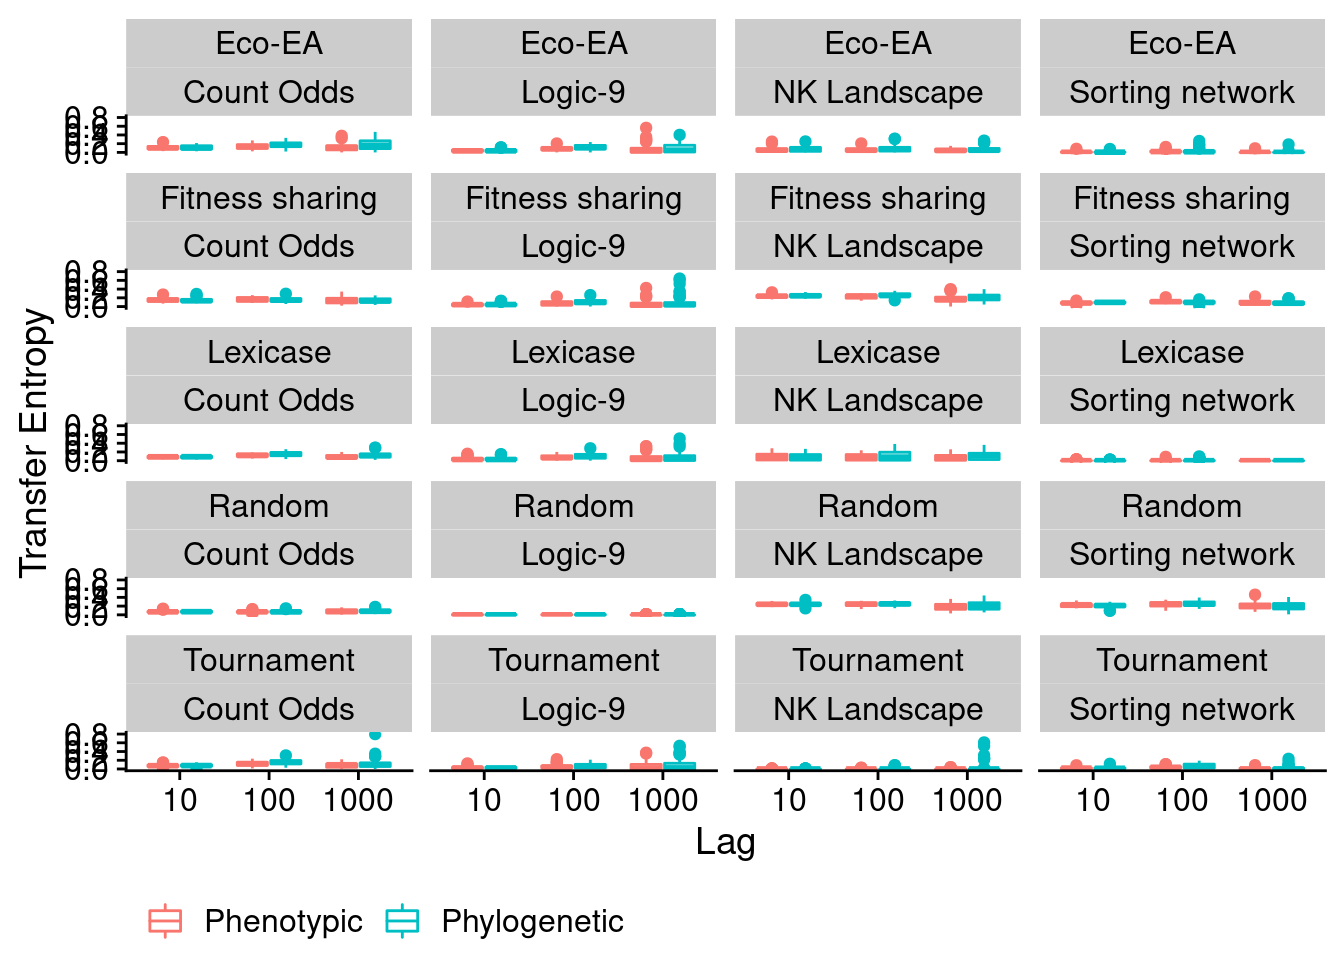
\includegraphics{phylodiversity-in-EC-supplement_files/figure-latex/complex_landscape_information_theory_variance_evolutionary_distinctivess-1.pdf}

\begin{Shaded}
\begin{Highlighting}[]
\NormalTok{res <-}\StringTok{ }\NormalTok{data }\OperatorTok\StringTok{ }\KeywordTok{group_by}\NormalTok{(SEED, selection_name, problem_name) }\OperatorTok
\KeywordTok{summarise}\NormalTok{(}
  \DataTypeTok{phen_phylo_10 =} \KeywordTok{condinformation}\NormalTok{(}\KeywordTok{discretize}\NormalTok{(phenotype_num_taxa), }\KeywordTok{discretize}\NormalTok{(}\KeywordTok{lag}\NormalTok{(max_phenotype_pairwise_distance, }\DecValTok{1}\NormalTok{)), }\KeywordTok{discretize}\NormalTok{(}\KeywordTok{lag}\NormalTok{(phenotype_num_taxa, }\DecValTok{1}\NormalTok{))),}
  \DataTypeTok{phen_phylo_100 =} \KeywordTok{condinformation}\NormalTok{(}\KeywordTok{discretize}\NormalTok{(phenotype_num_taxa), }\KeywordTok{discretize}\NormalTok{(}\KeywordTok{lag}\NormalTok{(max_phenotype_pairwise_distance, }\DecValTok{10}\NormalTok{)), }\KeywordTok{discretize}\NormalTok{(}\KeywordTok{lag}\NormalTok{(phenotype_num_taxa, }\DecValTok{10}\NormalTok{))),}
  \DataTypeTok{pheno_phylo_1000 =} \KeywordTok{condinformation}\NormalTok{(}\KeywordTok{discretize}\NormalTok{(phenotype_num_taxa), }\KeywordTok{discretize}\NormalTok{(}\KeywordTok{lag}\NormalTok{(max_phenotype_pairwise_distance, }\DecValTok{100}\NormalTok{)), }\KeywordTok{discretize}\NormalTok{(}\KeywordTok{lag}\NormalTok{(phenotype_num_taxa, }\DecValTok{100}\NormalTok{))),}
    \DataTypeTok{phylo_pheno_10 =} \KeywordTok{condinformation}\NormalTok{(}\KeywordTok{discretize}\NormalTok{(max_phenotype_pairwise_distance), }\KeywordTok{discretize}\NormalTok{(}\KeywordTok{lag}\NormalTok{(phenotype_num_taxa, }\DecValTok{1}\NormalTok{)), }\KeywordTok{discretize}\NormalTok{(}\KeywordTok{lag}\NormalTok{(max_phenotype_pairwise_distance, }\DecValTok{1}\NormalTok{))),}
      \DataTypeTok{phylo_pheno_100 =} \KeywordTok{condinformation}\NormalTok{(}\KeywordTok{discretize}\NormalTok{(max_phenotype_pairwise_distance), }\KeywordTok{discretize}\NormalTok{(}\KeywordTok{lag}\NormalTok{(phenotype_num_taxa, }\DecValTok{10}\NormalTok{)), }\KeywordTok{discretize}\NormalTok{(}\KeywordTok{lag}\NormalTok{(max_phenotype_pairwise_distance, }\DecValTok{10}\NormalTok{))),}
      \DataTypeTok{phylo_pheno_1000 =} \KeywordTok{condinformation}\NormalTok{(}\KeywordTok{discretize}\NormalTok{(max_phenotype_pairwise_distance), }\KeywordTok{discretize}\NormalTok{(}\KeywordTok{lag}\NormalTok{(phenotype_num_taxa, }\DecValTok{100}\NormalTok{)), }\KeywordTok{discretize}\NormalTok{(}\KeywordTok{lag}\NormalTok{(max_phenotype_pairwise_distance, }\DecValTok{100}\NormalTok{)))}
\NormalTok{      )}

\NormalTok{res <-}\StringTok{ }\NormalTok{res }\OperatorTok\StringTok{ }\KeywordTok{pivot_longer}\NormalTok{(}\DataTypeTok{cols=}\KeywordTok{contains}\NormalTok{(}\StringTok{"phylo"}\NormalTok{))}
\NormalTok{res}\OperatorTok{$}\NormalTok{offset <-}\StringTok{ }\KeywordTok{str_extract}\NormalTok{(res}\OperatorTok{$}\NormalTok{name, }\StringTok{"[:digit:]*$"}\NormalTok{)}
\NormalTok{res}\OperatorTok{$}\NormalTok{Type <-}\StringTok{ }\KeywordTok{case_when}\NormalTok{(}\KeywordTok{str_detect}\NormalTok{(res}\OperatorTok{$}\NormalTok{name, }\StringTok{"phylo_pheno"}\NormalTok{) }\OperatorTok{~}\StringTok{ "Phenotypic -> Phylogenetic"}\NormalTok{, }\OtherTok{TRUE} \OperatorTok{~}\StringTok{ "Phylogenetic -> Phenotypic"}\NormalTok{)}

\KeywordTok{ggplot}\NormalTok{(}
\NormalTok{  res, }
  \KeywordTok{aes}\NormalTok{(}
    \DataTypeTok{x=}\KeywordTok{as.factor}\NormalTok{(offset), }
    \DataTypeTok{y=}\NormalTok{value, }
    \DataTypeTok{color=}\NormalTok{Type}
\NormalTok{    )}
\NormalTok{  ) }\OperatorTok{+}\StringTok{ }
\StringTok{  }\KeywordTok{geom_boxplot}\NormalTok{() }\OperatorTok{+}\StringTok{ }
\StringTok{  }\KeywordTok{facet_wrap}\NormalTok{(}\OperatorTok{~}\NormalTok{problem_name}\OperatorTok{*}\NormalTok{selection_name) }\OperatorTok{+}\StringTok{ }
\StringTok{  }\KeywordTok{scale_x_discrete}\NormalTok{(}\StringTok{"Lag"}\NormalTok{) }\OperatorTok{+}\StringTok{ }
\StringTok{  }\KeywordTok{scale_y_continuous}\NormalTok{(}\StringTok{"Transfer Entropy"}\NormalTok{) }\OperatorTok{+}\StringTok{ }
\StringTok{  }\KeywordTok{scale_color_discrete}\NormalTok{(}\StringTok{""}\NormalTok{) }\OperatorTok{+}\StringTok{ }
\StringTok{  }\KeywordTok{theme}\NormalTok{(}\DataTypeTok{legend.position =} \StringTok{"bottom"}\NormalTok{)}
\end{Highlighting}
\end{Shaded}

\includegraphics{phylodiversity-in-EC-supplement_files/figure-latex/complex_landscape_information_theory_pheno_phylo-1.pdf}

\begin{Shaded}
\begin{Highlighting}[]
\NormalTok{res <-}\StringTok{ }\NormalTok{data }\OperatorTok\StringTok{ }\KeywordTok{group_by}\NormalTok{(SEED, selection_name, problem_name) }\OperatorTok
\KeywordTok{summarise}\NormalTok{(}
  \DataTypeTok{phen_phylo_10 =} \KeywordTok{condinformation}\NormalTok{(}\KeywordTok{discretize}\NormalTok{(phenotype_num_taxa), }\KeywordTok{discretize}\NormalTok{(}\KeywordTok{lag}\NormalTok{(max_phenotype_evolutionary_distinctiveness, }\DecValTok{1}\NormalTok{)), }\KeywordTok{discretize}\NormalTok{(}\KeywordTok{lag}\NormalTok{(phenotype_num_taxa, }\DecValTok{1}\NormalTok{))),}
  \DataTypeTok{phen_phylo_100 =} \KeywordTok{condinformation}\NormalTok{(}\KeywordTok{discretize}\NormalTok{(phenotype_num_taxa), }\KeywordTok{discretize}\NormalTok{(}\KeywordTok{lag}\NormalTok{(max_phenotype_evolutionary_distinctiveness, }\DecValTok{10}\NormalTok{)), }\KeywordTok{discretize}\NormalTok{(}\KeywordTok{lag}\NormalTok{(phenotype_num_taxa, }\DecValTok{10}\NormalTok{))),}
  \DataTypeTok{pheno_phylo_1000 =} \KeywordTok{condinformation}\NormalTok{(}\KeywordTok{discretize}\NormalTok{(phenotype_num_taxa), }\KeywordTok{discretize}\NormalTok{(}\KeywordTok{lag}\NormalTok{(max_phenotype_evolutionary_distinctiveness, }\DecValTok{100}\NormalTok{)), }\KeywordTok{discretize}\NormalTok{(}\KeywordTok{lag}\NormalTok{(phenotype_num_taxa, }\DecValTok{100}\NormalTok{))),}
    \DataTypeTok{phylo_pheno_10 =} \KeywordTok{condinformation}\NormalTok{(}\KeywordTok{discretize}\NormalTok{(max_phenotype_evolutionary_distinctiveness), }\KeywordTok{discretize}\NormalTok{(}\KeywordTok{lag}\NormalTok{(phenotype_num_taxa, }\DecValTok{1}\NormalTok{)), }\KeywordTok{discretize}\NormalTok{(}\KeywordTok{lag}\NormalTok{(max_phenotype_evolutionary_distinctiveness, }\DecValTok{1}\NormalTok{))),}
      \DataTypeTok{phylo_pheno_100 =} \KeywordTok{condinformation}\NormalTok{(}\KeywordTok{discretize}\NormalTok{(max_phenotype_evolutionary_distinctiveness), }\KeywordTok{discretize}\NormalTok{(}\KeywordTok{lag}\NormalTok{(phenotype_num_taxa, }\DecValTok{10}\NormalTok{)), }\KeywordTok{discretize}\NormalTok{(}\KeywordTok{lag}\NormalTok{(max_phenotype_evolutionary_distinctiveness, }\DecValTok{10}\NormalTok{))),}
      \DataTypeTok{phylo_pheno_1000 =} \KeywordTok{condinformation}\NormalTok{(}\KeywordTok{discretize}\NormalTok{(max_phenotype_evolutionary_distinctiveness), }\KeywordTok{discretize}\NormalTok{(}\KeywordTok{lag}\NormalTok{(phenotype_num_taxa, }\DecValTok{100}\NormalTok{)), }\KeywordTok{discretize}\NormalTok{(}\KeywordTok{lag}\NormalTok{(max_phenotype_evolutionary_distinctiveness, }\DecValTok{100}\NormalTok{)))}
\NormalTok{      )}

\NormalTok{res <-}\StringTok{ }\NormalTok{res }\OperatorTok\StringTok{ }\KeywordTok{pivot_longer}\NormalTok{(}\DataTypeTok{cols=}\KeywordTok{contains}\NormalTok{(}\StringTok{"phylo"}\NormalTok{))}
\NormalTok{res}\OperatorTok{$}\NormalTok{offset <-}\StringTok{ }\KeywordTok{str_extract}\NormalTok{(res}\OperatorTok{$}\NormalTok{name, }\StringTok{"[:digit:]*$"}\NormalTok{)}
\NormalTok{res}\OperatorTok{$}\NormalTok{Type <-}\StringTok{ }\KeywordTok{case_when}\NormalTok{(}\KeywordTok{str_detect}\NormalTok{(res}\OperatorTok{$}\NormalTok{name, }\StringTok{"phylo_pheno"}\NormalTok{) }\OperatorTok{~}\StringTok{ "Phenotypic -> Phylogenetic"}\NormalTok{, }\OtherTok{TRUE} \OperatorTok{~}\StringTok{ "Phylogenetic -> Phenotypic"}\NormalTok{)}

\KeywordTok{ggplot}\NormalTok{(}
\NormalTok{  res, }
  \KeywordTok{aes}\NormalTok{(}
    \DataTypeTok{x=}\KeywordTok{as.factor}\NormalTok{(offset), }
    \DataTypeTok{y=}\NormalTok{value, }
    \DataTypeTok{color=}\NormalTok{Type}
\NormalTok{    )}
\NormalTok{  ) }\OperatorTok{+}\StringTok{ }
\StringTok{  }\KeywordTok{geom_boxplot}\NormalTok{() }\OperatorTok{+}\StringTok{ }
\StringTok{  }\KeywordTok{facet_wrap}\NormalTok{(}\OperatorTok{~}\NormalTok{problem_name}\OperatorTok{*}\NormalTok{selection_name) }\OperatorTok{+}\StringTok{ }
\StringTok{  }\KeywordTok{scale_x_discrete}\NormalTok{(}\StringTok{"Lag"}\NormalTok{) }\OperatorTok{+}\StringTok{ }
\StringTok{  }\KeywordTok{scale_y_continuous}\NormalTok{(}\StringTok{"Transfer Entropy"}\NormalTok{) }\OperatorTok{+}\StringTok{ }
\StringTok{  }\KeywordTok{scale_color_discrete}\NormalTok{(}\StringTok{""}\NormalTok{) }\OperatorTok{+}\StringTok{ }
\StringTok{  }\KeywordTok{theme}\NormalTok{(}\DataTypeTok{legend.position =} \StringTok{"bottom"}\NormalTok{)}
\end{Highlighting}
\end{Shaded}

\includegraphics{phylodiversity-in-EC-supplement_files/figure-latex/complex_landscape_information_theory_pheno_phylo_evolutionary_distinctiveness-1.pdf}

\bibliography{book.bib,packages.bib}

\end{document}
